% author: Franz Taffner
% year: 2017
% institute: University of Graz

\documentclass[
a4paper, 
oneside,
12pt         % set default font size to 12 point
]{scrartcl} 

% inputenc: coding of german special characters
\usepackage[utf8]{inputenc}

\usepackage[english]{babel}
\usepackage{csquotes}
\usepackage[backend = biber, style=numeric-comp, sorting=none, natbib=true, maxbibnames=25, hyperref=true]{biblatex}
\addbibresource{_literature/literature.bib}



% fontenc, ae, aecompl: coding of characters in PDF documents
\usepackage[T1]{fontenc}
\usepackage{ae,aecompl}

% amsmath, amssymb, amstext: support for mathematics
\usepackage{amsmath,amssymb,amstext}

% units: technical units
\usepackage{units}

% LAYOUT

\usepackage{scrpage2}

%% PDF

\newif\ifpdf
\ifx\pdfoutput\undefined
\pdffalse
\else
\pdfoutput=1
\pdftrue
\fi

% definitions for using pdflatex instead of latex

\ifpdfoutput{

	\usepackage[pdftex]{graphicx}
	
	\pdfcompresslevel=9
	
	%hyperref (hyperlinks in PDF)

	\usepackage[	
	pdftex=true,
	backref=true,      
	pagebackref=false, 
	colorlinks=true,   
	bookmarks=true,          
	bookmarksopen=false,     
	bookmarksnumbered=false, 
	pdfpagemode=None         
	]{hyperref}

	\DeclareGraphicsExtensions{.pdf}
	
}{	
	\usepackage[dvips]{graphicx}
	
	\DeclareGraphicsExtensions{.eps}
	
	\usepackage[
	dvips,
	colorlinks=false
	]{hyperref}	
}

\usepackage{booktabs}

\usepackage{hyperref}
\hypersetup{
	pdftitle    = {GR-PAM with optical US detection},
	pdfauthor   = {Franz Taffner},
	pdfkeywords = {2017},linkcolor=blue
}

\newcommand{\mygraphics}[3]{
	\begin{center}
		\includegraphics[width=#1, keepaspectratio=true]{#2} \\
		\textbf{#3}
	\end{center}
}

\usepackage{scrpage2}
\pagestyle{scrheadings}
\usepackage{float}
\usepackage{tabu}
\usepackage{array}
\usepackage{multirow}
\usepackage{pdfpages} 
\usepackage{listings}
\usepackage[titletoc]{appendix}
\usepackage{longtable}
\usepackage{ifthen,changepage}

% DOKUMENT

\begin{document}

\renewcommand{\contentsname}{Table of contents}

\begingroup

	\thispagestyle{empty}
\begin{center}

\vspace*{0.5cm}

\begin{huge}
\color{blue}

Grueneisen relaxation photoacoustic microscopy (GR-PAM)

\end{huge}

\vspace*{3mm}

\Large{with optical ultrasonic detection}

\vspace*{1.5cm}

\huge{Master Thesis}

\vspace*{1cm}

\large

This thesis is submitted for the degree of\\
Master of Science (M.Sc) \\
by\\
\vspace*{5mm}
\Large\textbf{Franz Taffner}\\

\vspace*{5mm}

Department of Experimental Physics \\
at the Karl-Franzens-University of Graz

\vspace*{2cm}

Advisor: \\
Dr. rer. nat. Robert Nuster\\
Ao. Univ. Prof., Dr. G\"unther Paltauf

\vspace*{1cm}

Graz, January 2018\\
\vspace*{0.5cm}

\includegraphics[width=2.5cm]{00_coverpage/images/logo_uni_graz_4c.jpg} \\

\end{center}
\newpage
\thispagestyle{empty}
\section*{}
\newpage
\thispagestyle{empty}
\section*{Statutory Declaration}
\begin{flushleft}
I declare that I have authored this thesis independently that I have not used other than the declared sources or resources and that I have explicitly marked all material, which has been quoted literally or by content from the used sources.\\

\vspace*{2.5cm}

Graz, January 2018
\end{flushleft}
\newpage
\thispagestyle{empty}
\section*{}
\newpage

\section*{Danksagung}

Diese Masterarbeit w\"{a}re ohne die Unterst\"{u}tzung einiger Personen nicht m\"{o}glich geworden. Als erstes m\"{o}chte ich mich bei meinem Betreuer Dr. Robert Nuster bedanken. Er durfte sich mit den meisten meiner Fragen herumschlagen und stand mir immer geduldig mit Rat und Tat zur Seite.\\
Im gleichen Ma{\ss}e m\"{o}chte ich mich auch bei Dr. G\"{u}nther Paltauf bedanken, f\"{u}r die mir entgegen gebrachte Unterst\"{u}tzung.\\
Au{\ss}erdem m\"{o}chte ich mich noch bei der ganzen Arbeitsgruppe f\"{u}r die sehr unterhaltsamen Diskussionen und die Unterst\"{u}tzung bedanken.\\
Ein besonderer Dank gilt meinen Eltern die mir das Studium erm\"{o}glicht haben.\\
Vor allem m\"{o}chte ich mich noch bei meinen Freunden und meinem Bruder bedanken, die f\"{u}r die n\"{o}tige Ablenkung zum Studium sorgten.\\
Zum Schluss m\"{o}chte ich mich noch bei meiner Freundin Eva Fleischmann bedanken, die das Auf und Nieder des Studiums mit mir durchmachen durfte. F\"{u}r das „immer da sein“, die unz\"{a}hligen Korrekturen meiner sprachlichen Experimente und den glauben an mich, danke ich dir ganz besonders.
\newpage
\thispagestyle{empty}
\section*{}
\newpage
\thispagestyle{empty}
\section*{Abstract}

In search of new contrast mechanisms, the Grueneisen relaxation photoacoustic microscopy (GR-PAM) emerged in the field of photoacoustic microscopy. \\
In this thesis the underlaying effect, where the amplitude of the photoacoustic pressure wave changes due to a preheating, is proven. Furthermore, a comparison of GR-PAM to conventional optical resolution photoacoustic microscopy (OR-PAM) is done. \\
Additionally, a compact version of an optical ultrasonic transducer, based on a Fabry–P\'{e}rot interferometer, is constructed and built.\\

\section*{Kurzzusammenfassung}

Bei der Suche nach neuen Kontrastmechanismen entwickelte sich die Grueneisen Relaxations photoakustische Mikroskopie (GR-PAM) aus dem Feld der photoakustischen Mikroskopie heraus.
In dieser Arbeit wird dazu der zugrundeliegende Grueneiseneffekt bewiesen. Dabei ändert sich die Amplitude einer Druckwelle aufgrund eines vorhergehenden Aufheizens. Des Weiteren wird GR-PAM mit der optisch aufgelösten photoakustischen Mikroskopie (OR-PAM) verglichen. 
Zusätzlich wird ein System zur optischen Ultraschall Erkennung, basierend auf einem Fabry–P\'{e}rot Interferometer, entwickelt.  

\newpage
\thispagestyle{empty}
\section*{}



	\pagestyle{empty}
	\tableofcontents 
	\clearpage	
\endgroup

\begingroup

\pagestyle{plain}

\setcounter{page}{1}
\section{Introduction}

In todays medical diagnosis a lot of different imaging technologies are available to determine and examine various types of diseases. Whether it is magnetic resonance tomography (MRT), to display organs and tissue, or optical microscopy to figure out bacteria. At some point, for example in conventional microscopy, it is a necessity to use contrast agents to make things visible or in case of MRT, it is to expansive to gain benefit from it \cite{grun:integrating}. In order to meet this facts and overcome drawbacks the field of photoacoustic imaging is an very uprising field in medical diagnostics. The detected value is not back scattered or transmitted light, but a pressure wave generated by the sample itself through the interaction with light. This makes it a method with a lot of possibilities, too. Furthermore, it is non-invasive because the needed light intensity is below the damage threshold of biological materials. \\
Another advantage is the use of natural contrast agents such as melanin or hemoglobin. Due to the contrast mechanism is founded in the difference of the optical absorption~coefficient~$\mu_a$. Based on this effect two main fields have emerged, the photoacoustic microscopy (PAM) and the photoacoustic tomography (PAT) \cite{YAO201487}. \\
\\
This thesis focuses on two topics in the field of photoacoustic microscopy. At the beginning the photoacoustic effect and its technical realization in optical resolution photoacoustic microscopy (OR-PAM) gets described as state of the art technique. \\
Afterwards the Grueneisen effect and its application to microscopy, called Grueneisen relaxation photoacoustic microscopy (GR-PAM), gets introduced. Including a prove of the effect and an analysis of GR-PAM versus OR-PAM in view of additional contrast capabilities and sectioning qualities. The measurements are performed ex-vivo.\\
The second part of the thesis presents the construction and characterization of an optical ultrasonic transducer system. The described system is a further development of the one described by Gratt \cite{GrattSibylle:Dis} with focus on building a compact and movable system.\\


\section{Principles of photoacoustics}

For a basic understanding, this section will give a short introduction into the underlying photoacoustic effect and continues with its applications to microscopy. Furthermore, the used setup for the measurements gets discussed.

\subsection{Photoacoustic effect}
\label{sec:photoeffect}
The generation of a photoacoustic wave due to the illumination of a sample with temporal modulated light follows the process shown in Figure \ref{fig:PAgen} \cite{Wang:PAMtutorial}. 

\begin{figure}[H]
	\centering
	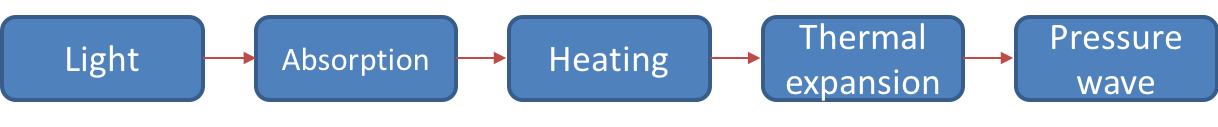
\includegraphics[width = 0.9\textwidth]{02_principles_of_photoacoustics/images/photoacousticGeneration.png}
	\caption{Sequence of the photoacoustic generation process.}
	\label{fig:PAgen}
\end{figure}

Light, for example a laser beam, hits a sample. The laser power can be written as

\begin{equation}
	P_{laser} = \frac{Q_{laser}}{\tau_{laser}}
	\label{eq:LP}
\end{equation}
\\
where $Q_{laser}$ is the laser pulse energy and $\tau_{laser}$ is the pulse duration. With the illuminated area $A_{laser}$ given by the laser beam diameter $d_{laser}$ follows the irradiance 

\begin{equation}
I_{laser} = \frac{4 \cdot P_{laser}}{d_{laser}^2 \cdot \pi} = \frac{P_{laser}}{A_{laser}}
\label{eq:ILaser}
\end{equation}
\\
it is assumed, that the sample surface is much bigger than the illuminated area. 

\begin{figure}[H]
	\centering
	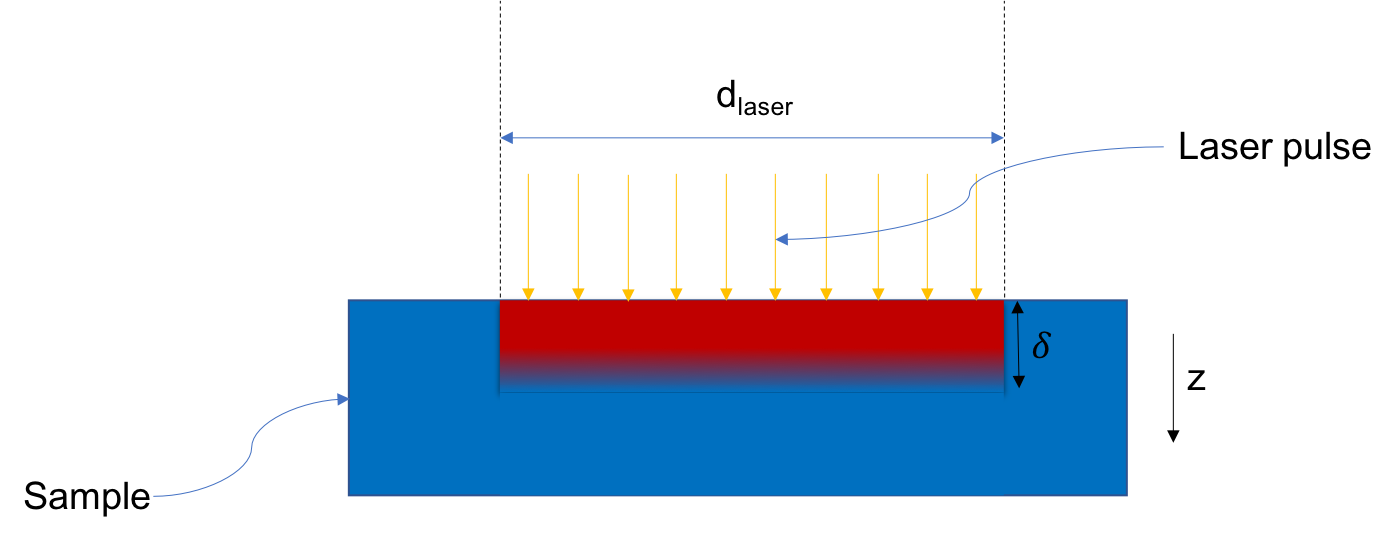
\includegraphics[width = 0.9\textwidth]{02_principles_of_photoacoustics/images/lpOnSample.png}
	\caption{Schematic view of a laser pulse hitting a sample.}
	\label{fig:LPonSample}
\end{figure}

The description of the absorption that happens subsequently is given by the Lambert-Beers law \cite{demtroder:ExPhysik}. Therefore, the depth profile of the irradiated intensity is defined by

 \begin{equation}
 	I(z) = I_{laser}  \cdot exp(-\mu_a \cdot z)
 	\label{eq:lambertbeer}
 \end{equation}
\\
where $\mu_a$ is the optical absorption coefficient of a non-scattering material. It describes the weakening of an incident electromagnetic wave. Furthermore, a penetration depth $\delta = \frac{1}{\mu_a}$, shown in Figure \ref{fig:LPonSample}, is defined by the intensity drop of $\frac{1}{e}$.\\
In the next step the absorbed light is converted into mechanical stress. For non-fluorescent materials it can be supposed, that the whole electromagnetic energy is converted into thermal energy and if the following two conditions are fulfilled, this energy will form an acoustic wave.\\
Whenever the energy is confined into the irradiated volume and does not vanish due to heat conduction, the "heat confinement" is achieved. This means that the laser pulse $\tau_{laser}$ is shorter than the thermal relaxation time $\tau_{th}$
given by
\begin{equation}
	\tau_{laser} < \tau_{th} = \frac{\delta'^2}{4\cdot\lambda_t} 
	\label{eq:thConf}
\end{equation}
\\
where $\delta'$ is the smallest dimension of the illuminated volume (laser beam diameter or penetration depth) and $\lambda_t$ is the thermal diffusivity. \newline
The second requirement for an efficient photoacoustic excitation process is to fulfill the condition for “stress confinement” defined by

\begin{equation}
t_{laser} < t_{ac} = \frac{\delta'}{c_s} 
\label{eq:stressConf}
\end{equation}
\\
where $c_s$ is the speed of sound in the medium. This condition ensures that no acoustic relaxation occurs during the excitation process. In either case (heat or stress confinement) a pressure rise, in reference to the equilibrium pressure, is achieved \cite{GrattSibylle:Dis}. 

\begin{equation}
\Delta p = - B \frac{\Delta V}{V}  + B \beta \Delta T
\label{eq:dV/V}
\end{equation}
\begin{equation}
B = \rho_0 c_s^2
\end{equation}
\\
where $B$ is the bulk modulus, $\rho_0$ the density at ambient pressure and $\beta$ the volume expansion coefficient. \\
Due to a laser excitation, the fractional volume expansion is negligible. From this follows an initial pressure rise of

\begin{equation}
p_0 =  B \beta \Delta T = \Gamma \mu_a F
\label{eq:p_0}
\end{equation}
\\
with 

\begin{equation}
\Delta T =  \frac{1}{C_V \cdot \rho } \cdot F \cdot \mu_a 
\label{eq:deltaT} 
\end{equation}
\begin{equation}
\Gamma =  \frac{B \cdot \beta}{\rho \cdot C_V} = \frac{\beta \cdot c_s^2}{C_P}
\end{equation}
\\
$F$...Fluence [J/m$^2$]\\
$C_V$...Heat capacity at constant volume [J/K]\\
$C_P$...Heat capacity at constant pressure [J/K]\\
$\rho$...Density [kg/m$^3$]\\
$\Gamma$...Grueneisenparameter\\\\

The Grueneisenparameter is temperature dependent.  Its property is discussed in chapter \ref{sec:GReffect}. The initial pressure rise relaxes and spreads out as an ultrasonic wave, which can be detected by an ultrasonic transducer \cite{GraflMonika2015Pm, doi:10.1021/cr010436c, WangLihongV2012BO:P}.

\subsection{Generation and propagation of photoacoustic waves}

The general photoacoustic equation is \cite{Wang:PAMtutorial}

\begin{equation}
	\left( \nabla^2 - \frac{1}{c_s^2} \frac{\partial^2}{\partial t^2}\right)p(\vec{r},t) = - \frac{\beta}{\kappa c_s^2}\frac{\partial^2T(\vec{r},t)}{\partial t^2}
	\label{eq:generalPA}
\end{equation}

with

\begin{equation}
	\kappa = \frac{C_P}{\rho c_s^2 C_V}
\end{equation}
\\
where $T$ is the temperature rise, $\kappa$ the isothermal compressibility and $p(\vec{r},t)$ the acoustic pressure at position $\vec{r}$ and time $t$. Equation \ref{eq:generalPA} contains a source term on the right side and a wave propagation term on the left.\\
If a laserpulse fulfills the terms for heat and stress confinement the heating function can be expressed as

\begin{equation}
	H(\vec{r},t) = \rho C_v \frac{\partial T(\vec{r},t)}{\partial t} = \mu_a F
\end{equation}
\\
This follows with equation \ref{eq:generalPA} and the source term, in this case $H$, a time derivative related equation. 

\begin{equation}
		\left( \nabla^2 - \frac{1}{c_s^2} \frac{\partial^2}{\partial t^2}\right)p(\vec{r},t) = - \frac{\beta}{C_p}\frac{\partial H(\vec{r},t)}{\partial t}
\end{equation}
\\
Therefore, only time-variant heating produces a pressure wave. The general photoacoustic equation \ref{eq:generalPA} can be solved by the Green's function approach. This leads to

\begin{equation}
	p(\vec{r},t) = \frac{\beta}{4 \pi C_p} \int \mathrm{d} \vec{r}\,^{'} \frac{1}{\vert \vec{r} - \vec{r}\,^{'} \vert} \frac{\partial H(\vec{r}\,^{'}, t^{'})}{\partial t^{'}} \Bigg|_{ t^{'}=t-\frac{\vert \vec{r}-\vec{r}\,^{'} \vert}{c_s}}
\end{equation} 
\\
where $\vec{r}\,^{'}$ and $t^{'}$ are the location and time  of the source. If $H(t^{'}) = \delta (t^{'})$, $p(\vec{r},t)$ can be written as

\begin{equation}
	p(\vec{r},t) = \frac{1}{4 \pi c_s^2} \frac{\partial}{\partial t} \left[ \frac{1}{c_s t} \int \mathrm{d}\vec{r}\,^{'} p_0(\vec{r}\,^{'}) \delta \left(t-\frac{\vert \vec{r} - \vec{r}\,^{'}\vert}{c_s}\right)\right]
	\label{eq:PAgenArb}
\end{equation}
\\
the square brackets yield a step heating response to an arbitrary absorbing object and its time differentiation follows the delta-heating response. Equation \ref{eq:PAgenArb} can be used to calculate photoacoustic pressure, generated by an heterogeneous optically absorbing object \cite{Wang:PAMtutorial}.\\

\subsubsection{Spherical-source solution and point detector}

The solution for a absorbing spherical object with radius $R_s$, that is homogeneously heated by a delta pulse is

\begin{equation}
p(r,t) = p_0 \left[\theta(R_s - c_s -r) + \frac{r-c_s t}{2r} \theta(r-\vert R_s - c_s t\vert) \theta(R_s + c_s t - r)\right]
\label{eq:prt}
\end{equation}
\\
where 

\begin{equation}
\theta(z) =
\begin{cases}
1 &  \mathrm{for}~z \geq 1\\
0 & \mathrm{else}
\end{cases}
\label{eq:theta}
\end{equation}
\\
the origin of $r$ is the center of the sphere. For an initial pressure of

\begin{equation}
p_0(r) = p_0\theta(r)\theta(-r + R_s);\;\;\;with~ 0\le r < R_s
\end{equation}
\\
formula \ref{eq:prt} becomes

\begin{equation}
p(r,t) = \underbrace{p_0(r+c_st) \cdot \frac{r+c_s t}{2r}}_{\mathrm{I}}+ \underbrace{p_0(-r+c_st) \cdot \frac{r-c_s t}{2r}}_{\mathrm{II}}+\underbrace{p_0(r-c_st) \cdot \frac{r-c_s t}{2r}}_{\mathrm{III}}
\label{eq:p0rt}
\end{equation}
\\
where part I is a converging spherical wave, part II is a radiating spherical wave excited by the converging wave of part I through the center and part III is a radiating spherical wave \cite{Wang:PAMtutorial}.\\
As the converging part I does not propagate outside of the sphere formula \ref{eq:p0rt} reduces into

\begin{equation}
p(z,t) = \frac{z-c_s t}{2z} p_0(-z+c_s t) + \frac{z-c_s t}{2z} p_0(z-c_s t)
\label{eq:p0rtdelta}
\end{equation}
\\
where the pressure wave is detected by a point like ultrasonic transducer, that is placed at distance $z$ outside the spherical source with given source radius $R_s$. \\
Figure \ref{fig:nShape} shows a simulation done with equation \ref{eq:p0rtdelta}.

\begin{figure}[H]
	\centering
	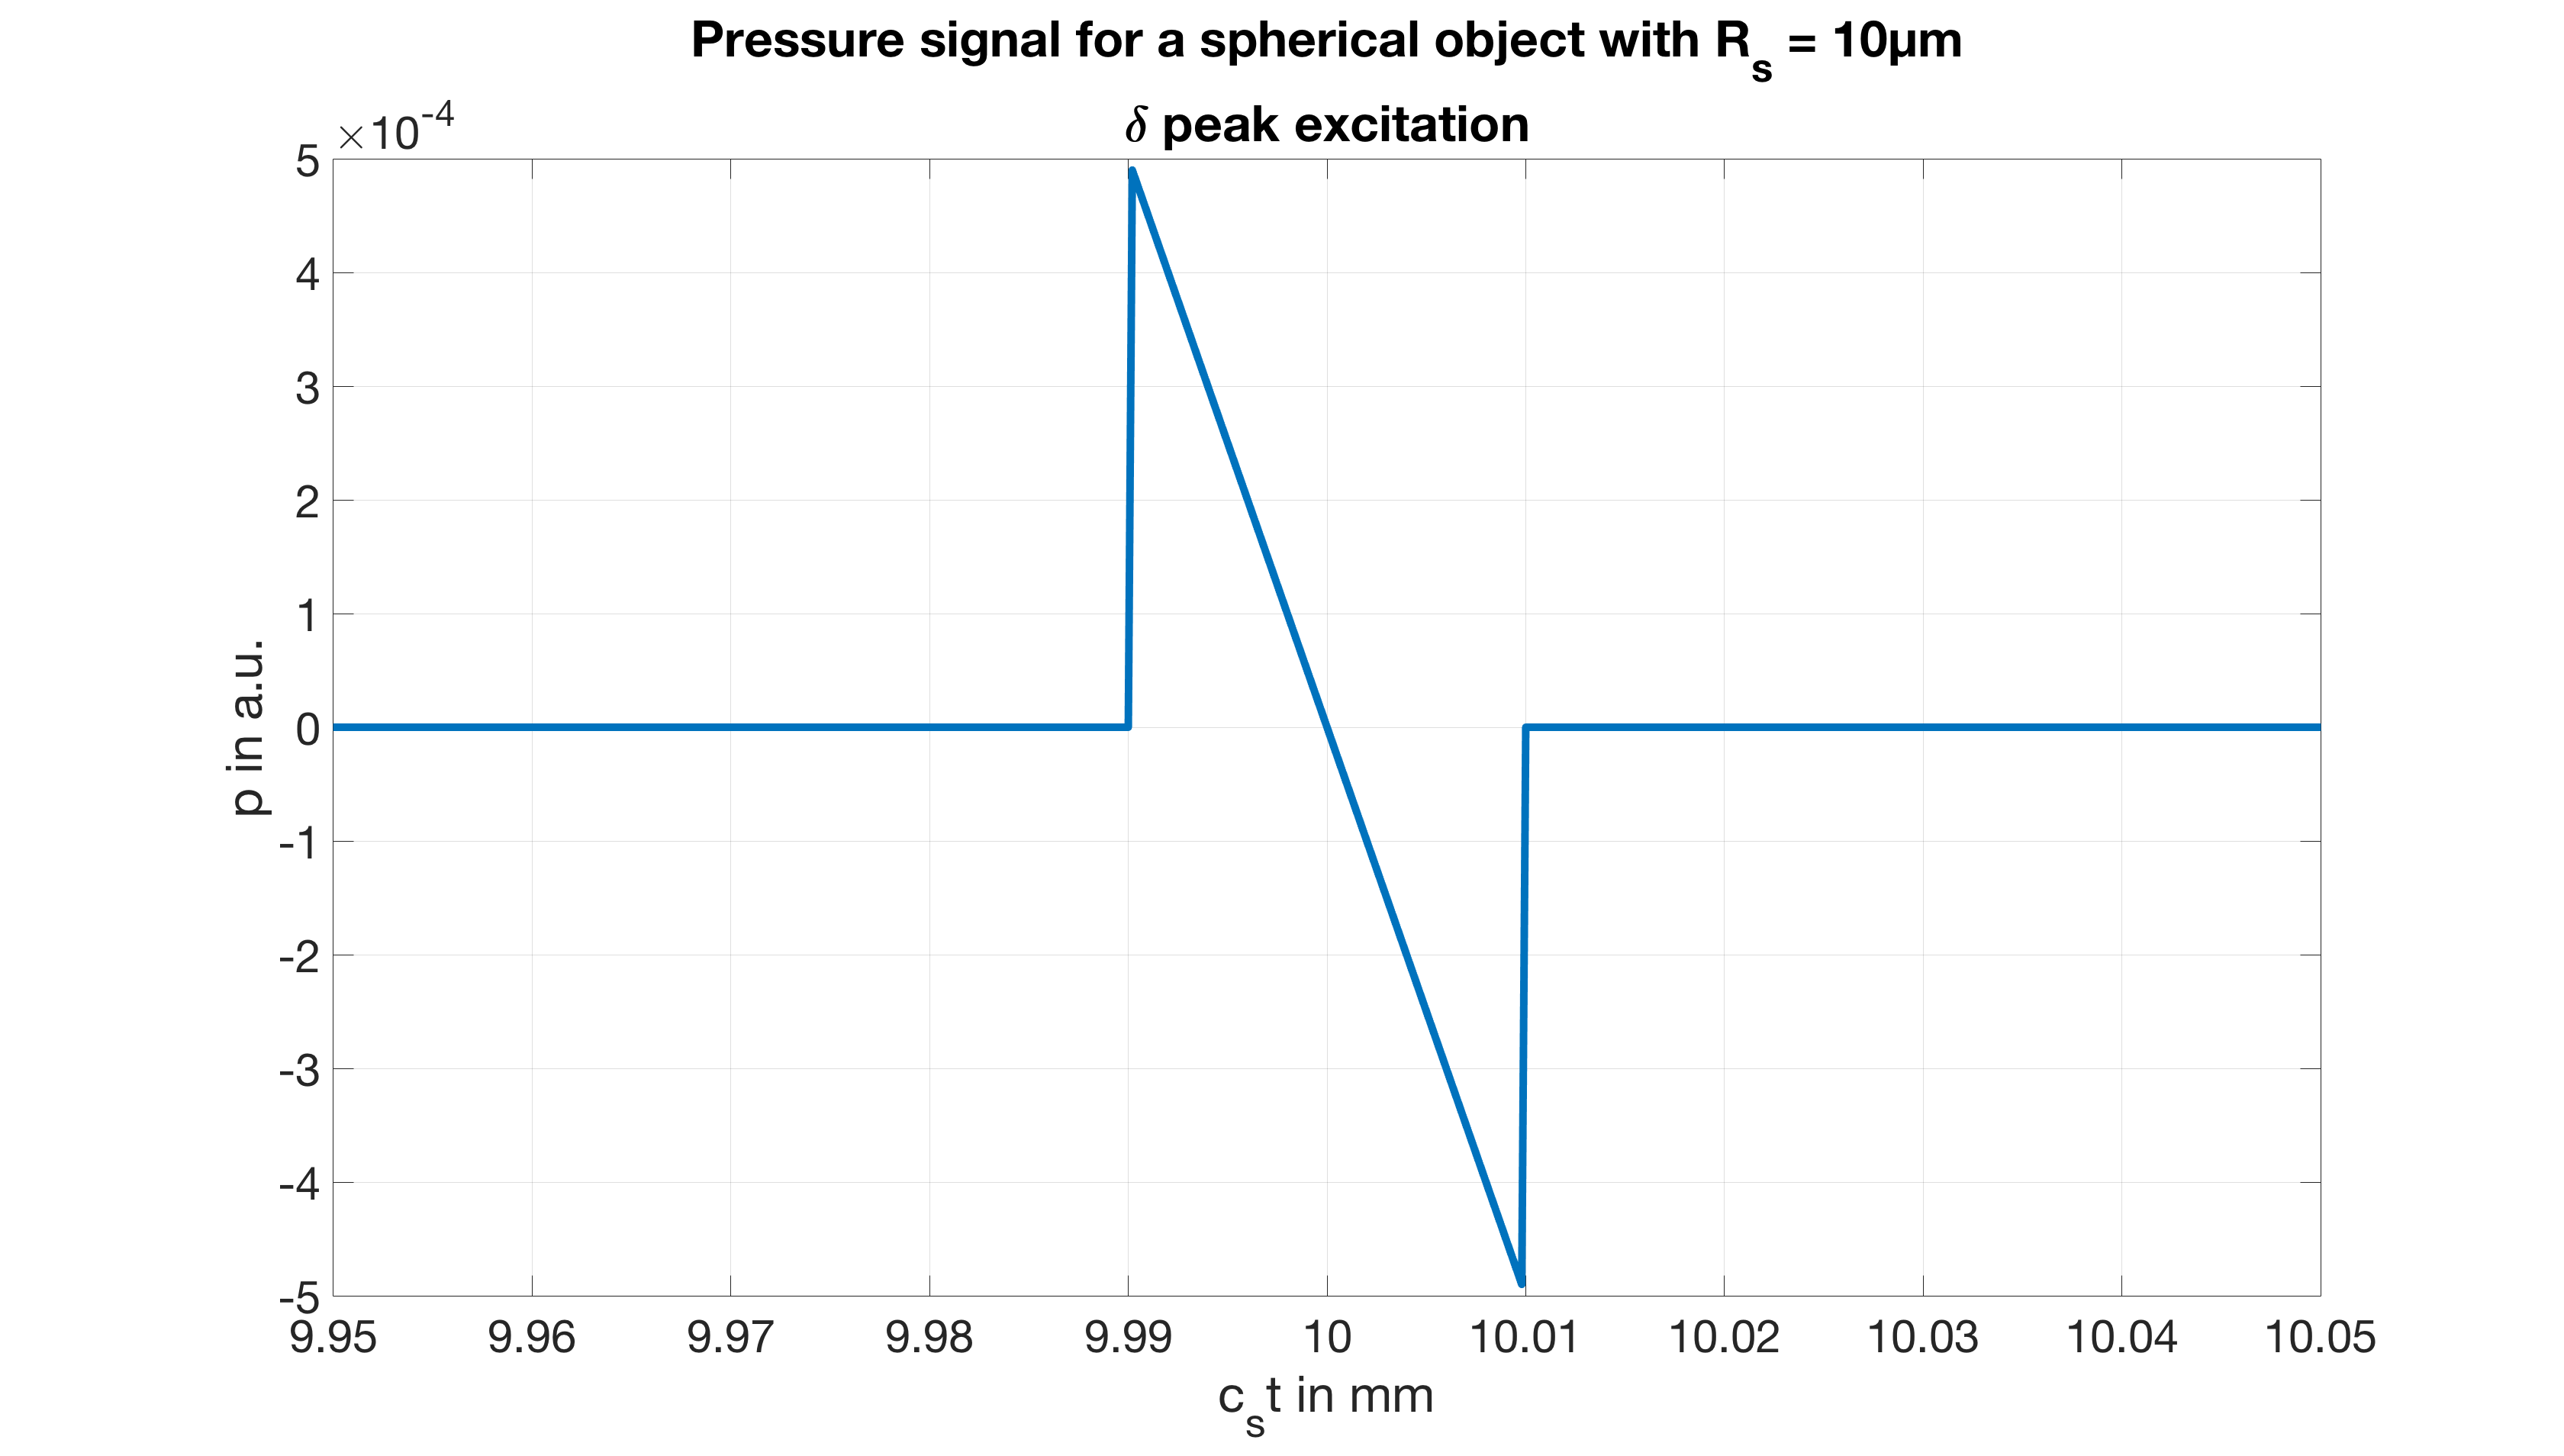
\includegraphics[width = 0.7\textwidth, height=0.3\textheight]{02_principles_of_photoacoustics/images/nShape.png}
	\caption{N-shape signal for a spherical source with $R_s$ = 10~$\mu m$, in $z$ = 10~$mm$ distance and $\delta$ pulse excitation (The calculation program can be found in appendix \ref{app:PAgen}).}
	\label{fig:nShape}
\end{figure}

\subsubsection{Spherical-source solution and finite detector}

The detection of a spherical propagating pressure wave with a pointlike ultrasonic detector corresponds to a convolution of the pressure signal function with a $\delta$-function. Hence the response of a ultrasonic transducer, with finite detection bandwidth, to a spherical pressure wave, can be calculated by a convolution of their time domain functions.\\
In figure \ref{fig:freqTimePAsig} a simulation is done with the parameters given above for the pressure wave excitation. The ultrasonic transducer is modulated by a Gaussian function in the frequency domain, with a center frequency of 50~$MHz$ and 70~$\%$ bandwidth.  

\begin{figure}[H]
	a)
	\begin{minipage}{0.5\textwidth}		
		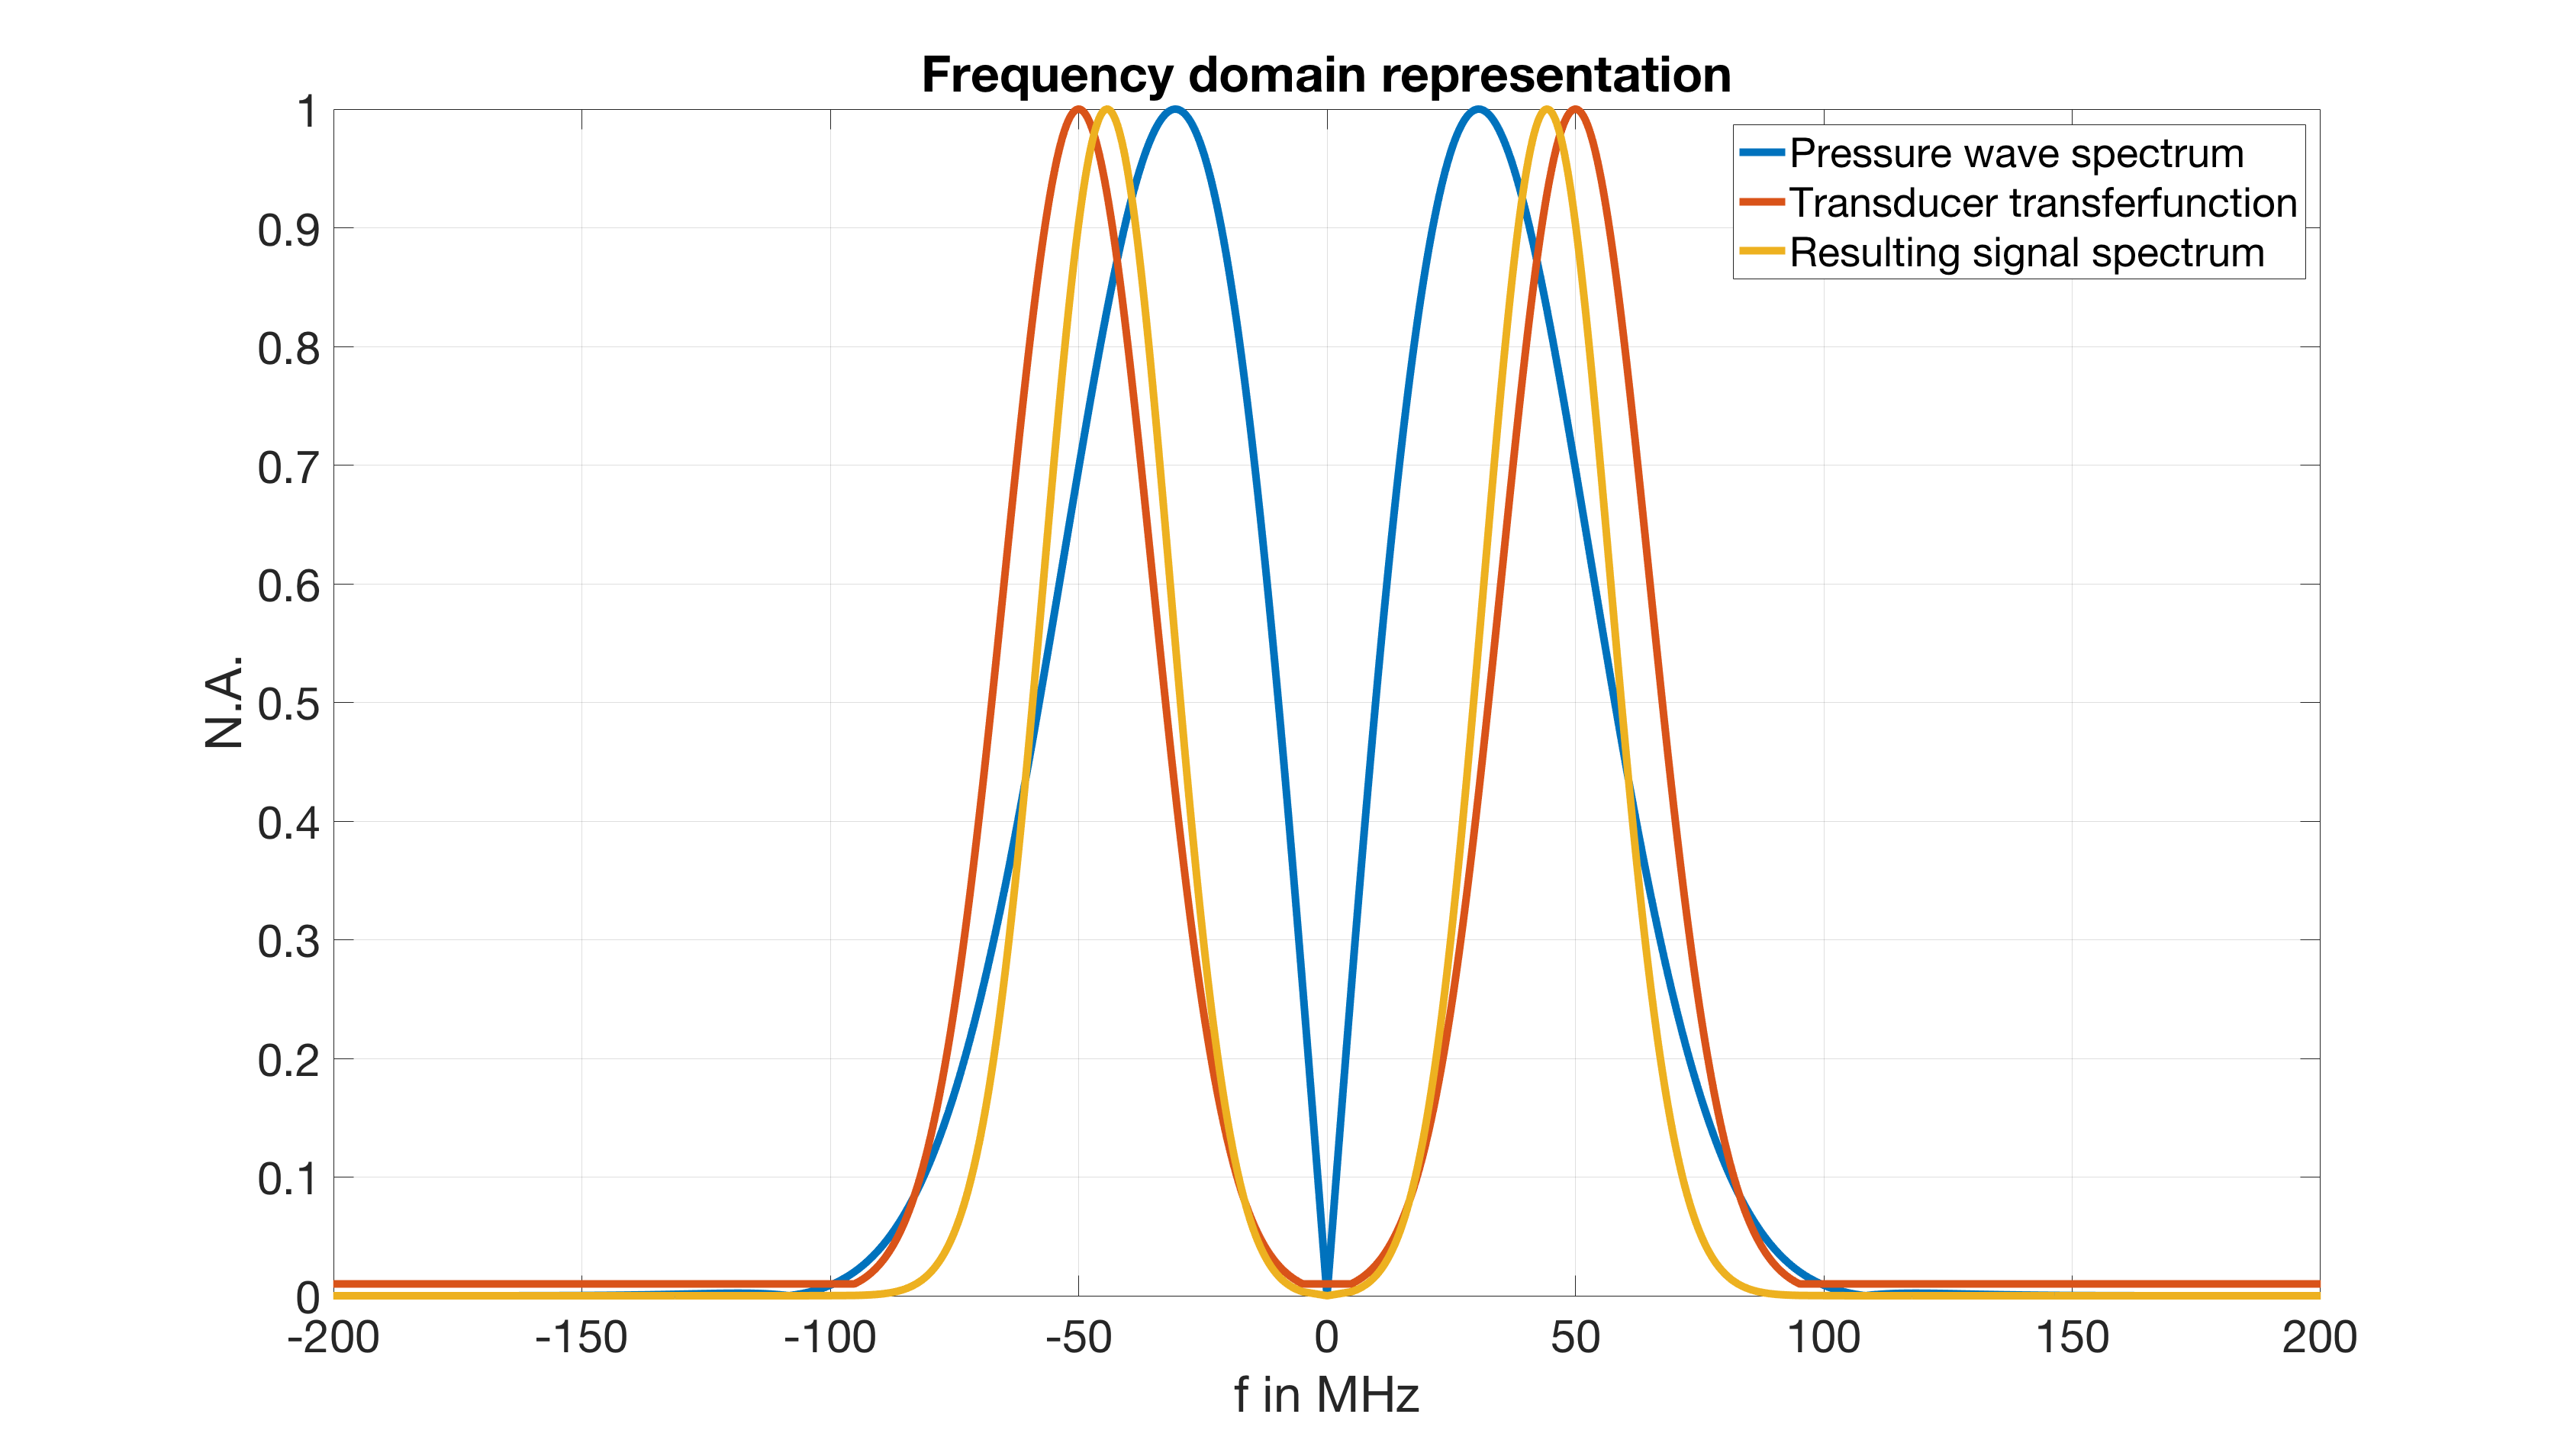
\includegraphics[width = \textwidth, height=0.25\textheight]{02_principles_of_photoacoustics/images/freqSphericalDet.png}
	\end{minipage}
	b)
	\begin{minipage}{0.5\textwidth}		
		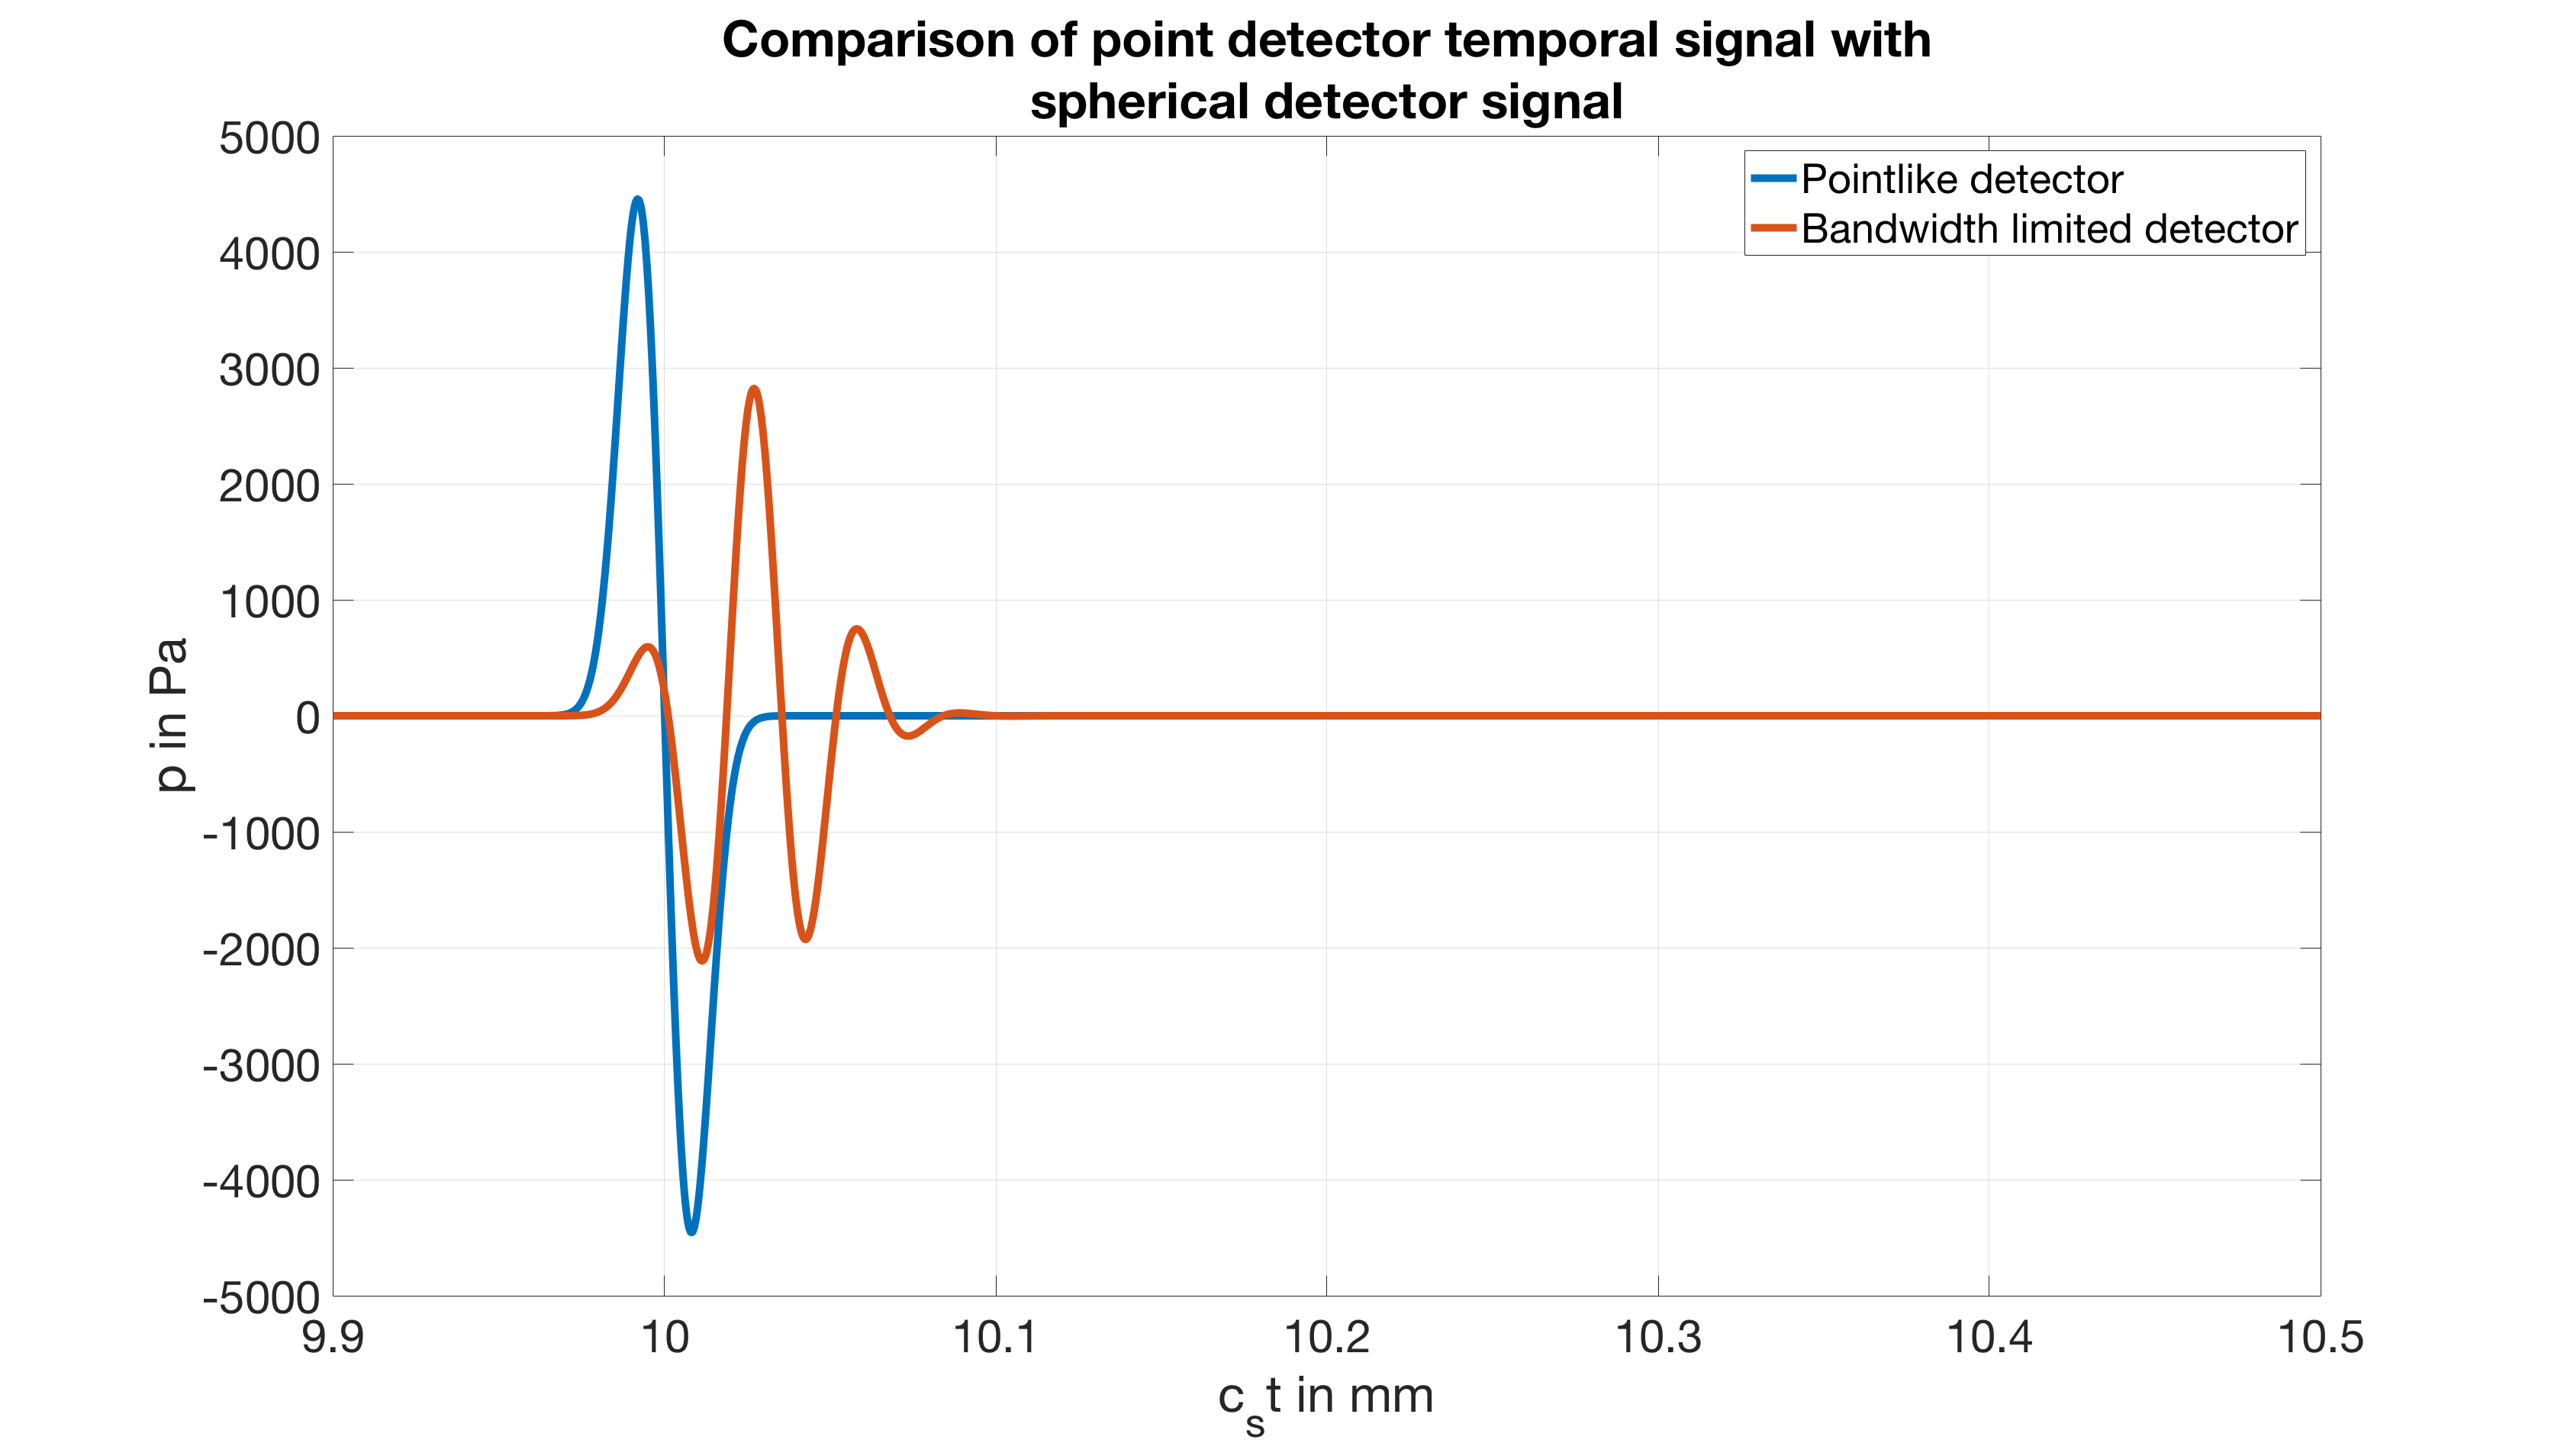
\includegraphics[width = \textwidth, height=0.25\textheight]{02_principles_of_photoacoustics/images/timeSphericalDet.png}
	\end{minipage}	
	\caption{In a) the frequency domain representation of the ultrasonic transferfunction, the source signal function and the resulting signal are shown. The time domain functions, of a pressure wave detected by a pointlike (blue-line) and a bandwidth limited ultrasonic transducer (orange-line), are shown in b). The used code can be found in appendix \ref{app:PAgen}.}
	\label{fig:freqTimePAsig}
\end{figure} 

The simulation clearly shows the impact of the limited bandwidth of the ultrasonic transducer. For comparison, a response function of a real detected signal is shown in figure \ref{fig:PAhilbertSim}. Both show the typical symmetric shape. 

\subsubsection{Study on ultrasonic transducer center frequency}

Based on the previous considerations the impact of the center frequency of a ultrasonic transducer on the maximum amplitude for different source diameter is studied.\\
Three source diameter are studied, 5~$\mu m$, 10~$\mu m$ and 20~$\mu m$. The simulation range for the transducer center frequency is 1 to 100~$MHz$ with a bandwidth of $0.7 \cdot f_{center}$. Therefore not just the value for the center frequency increases, also the bandwidth. The simulation result is shown in figure \ref{fig:centerFreq}.

\begin{figure}[H]
	\centering
	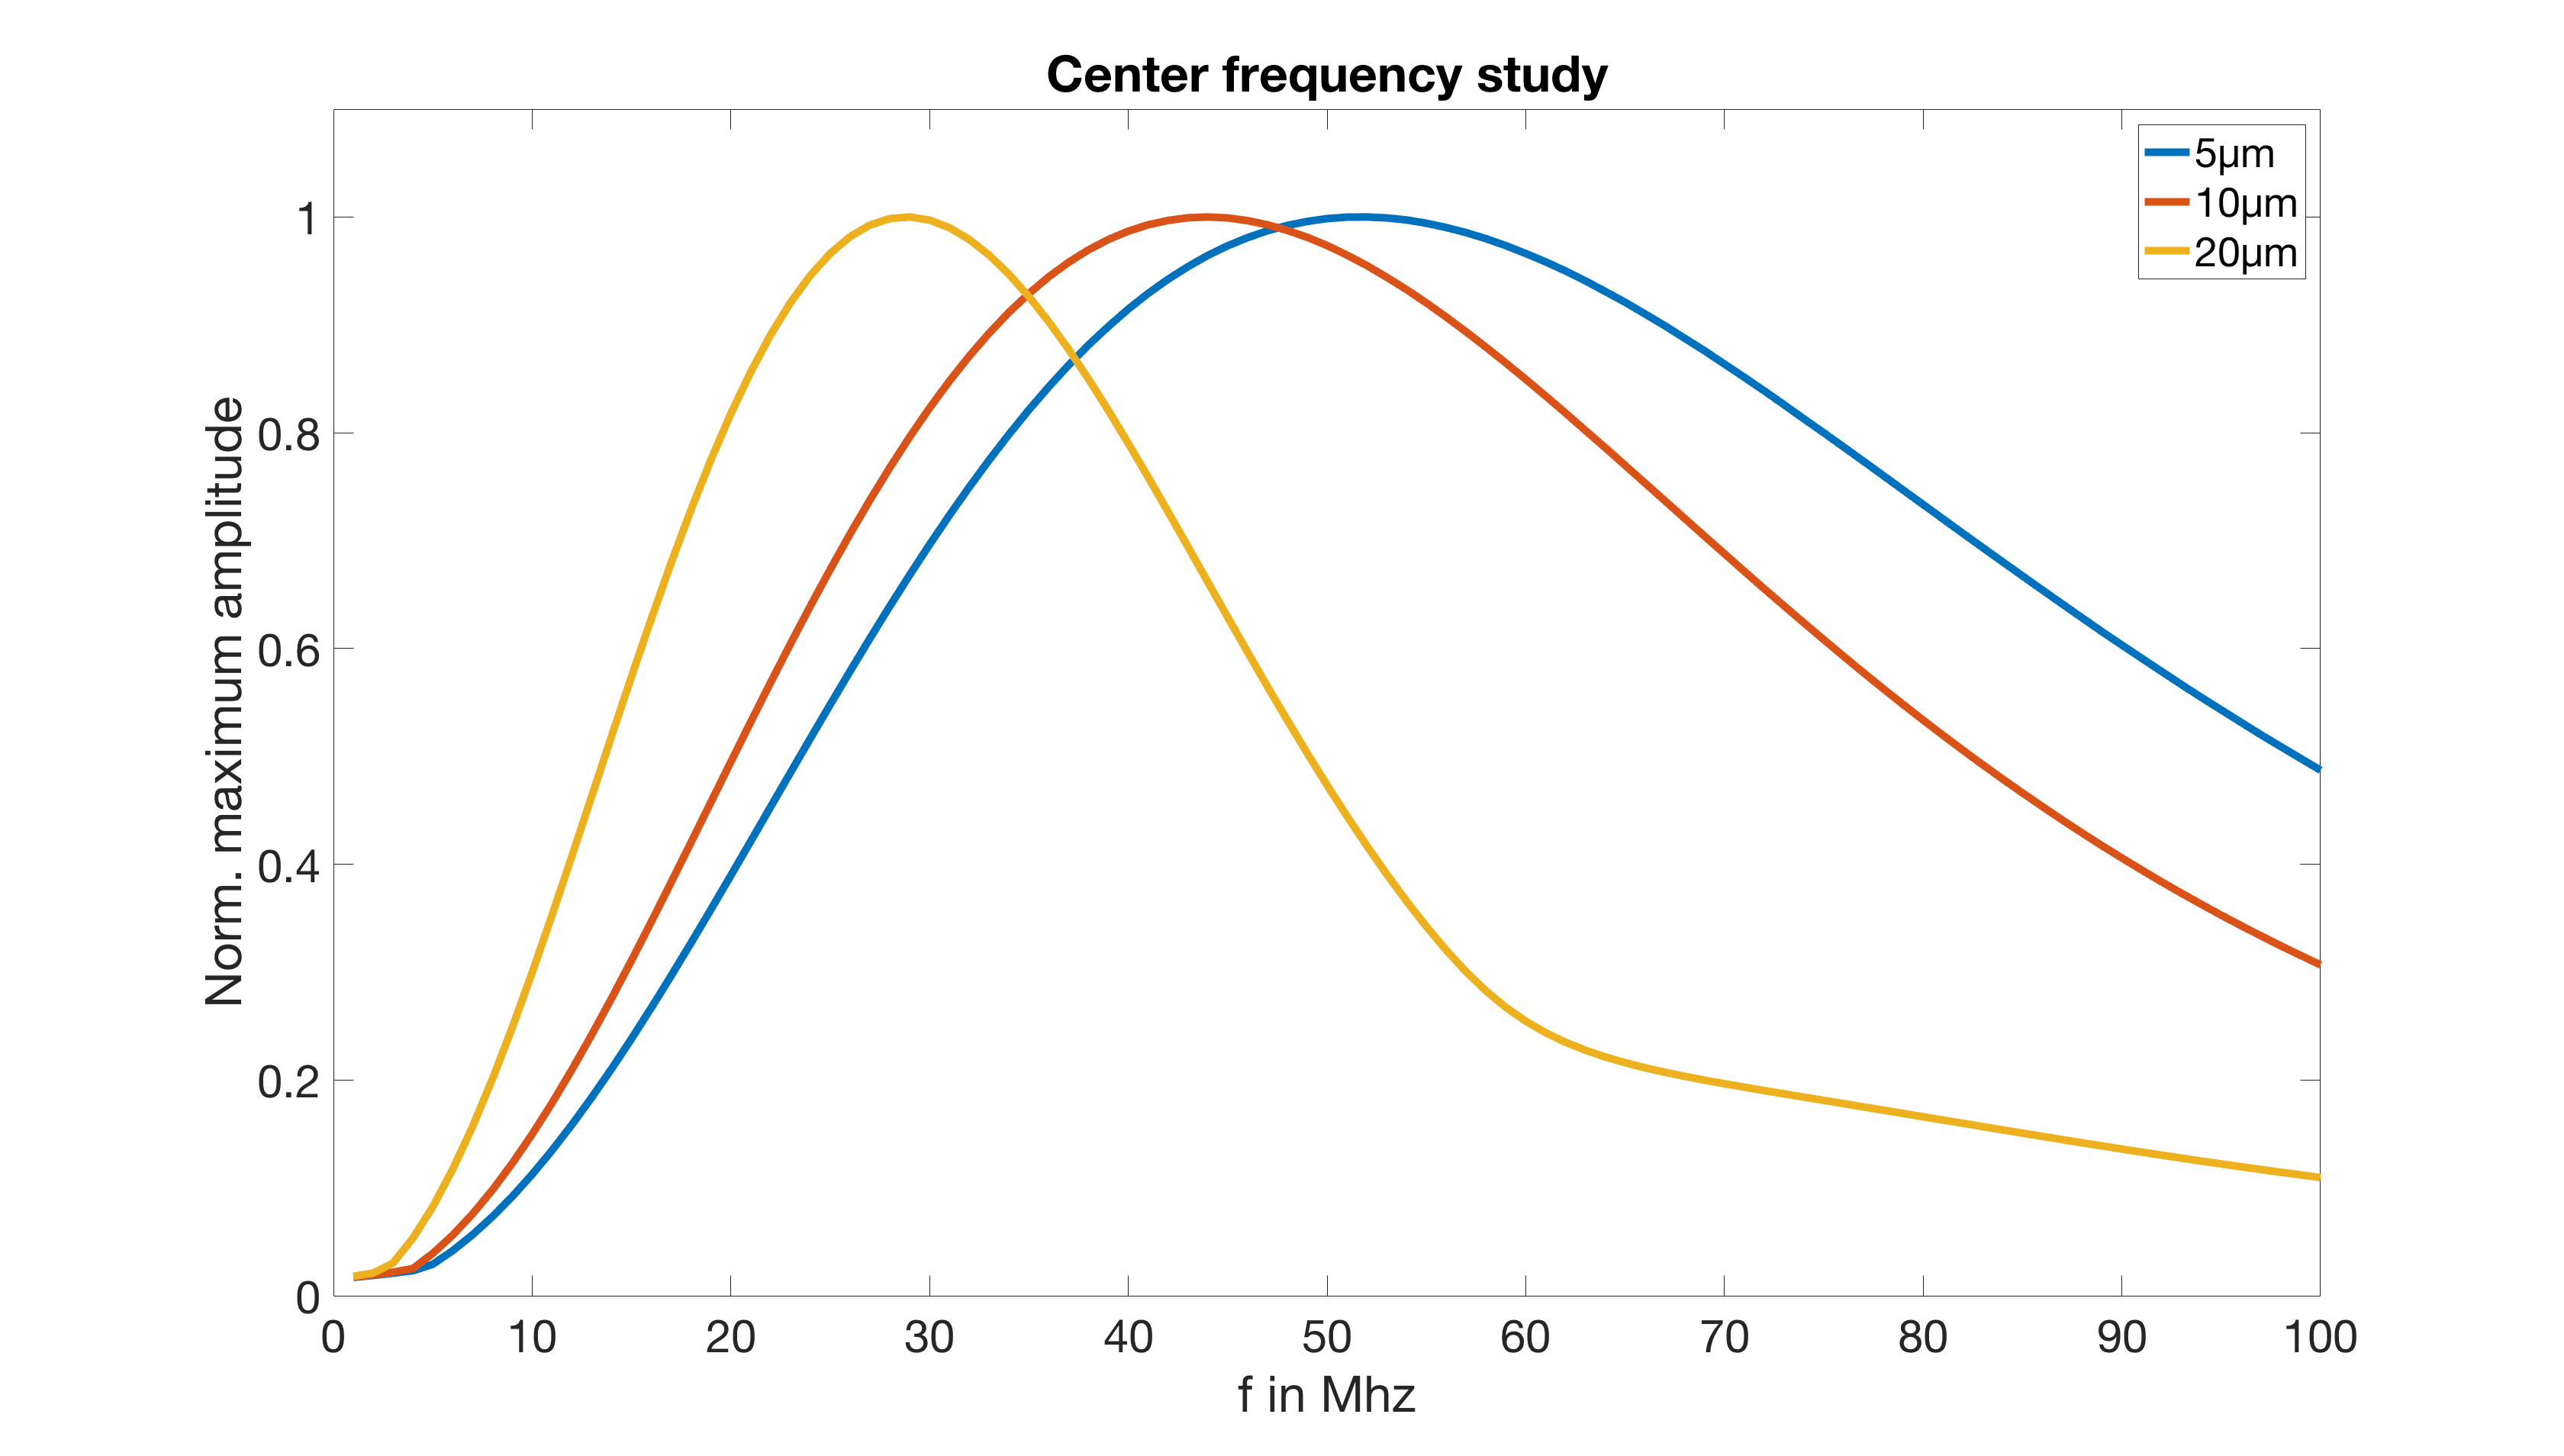
\includegraphics[width = 0.7\textwidth, height=0.3\textheight]{02_principles_of_photoacoustics/images/centerFreq.png}
	\caption{Simulated maximum amplitude response for a 5~$\mu m$, 10~$\mu m$ and 20~$\mu m$ source in dependence of the center frequency of the ultrasonic transducer. The transducers are modeled with a bandwidth of $0.7 \cdot f_{center}$.}
	\label{fig:centerFreq}
\end{figure}

The maximum amplitude values are once more normalized to the maximum possible signal value, for each source diameter.\\
It can be seen that smaller sources produce higher frequency ratios. Therefore it is necessary to use ultrasonic transducer with a high center frequency to image small details.\\
On the other hand the full dimension of bigger sources is only observable if the transducer bandwidth contains lower frequencies, too. For the  20~$\mu m$ source in figure \ref{fig:centerFreq}, a ultrasonic transducer with a center frequency of 29~$MHz$ would be the perfect choice.\\
The source sizes, that should be observed, are in the range of 5 to 10~$\mu m$, therefore a transducer with 50~$MHz$ center frequency and $0.7 \cdot f_{center}$ is chosen.  

\subsection{Photoacoustic microscopy}

On the basis of the photoacoustic effect several applications have emerged. For example microscopy and tomography of biological specimen. \\
In photoacoustic tomography (PAT), the whole area of interest is illuminated. An array of ultrasonic transducers is placed around the sample to receive the excited ultrasonic waves. With the information of how much optical energy was placed onto the sample, the ultrasonic signal coming from different directions and a reconstruction algorithm, a 3D image can be generated. \\
Photoacoustic microscopy (PAM) on the other hand takes one record at a time (A-scan) and generates a picture by scanning over the sample. There are two common methods to do PAM. In acoustical resolution PAM (AR-PAM) a broadened laser beam hits a sample and the generated ultrasonic wave is detected by an ultrasonic detector with focusing properties. The other feasibility is to focus the laser beam onto a sample, so-called OR-PAM, which is discussed in the following, as it is the basis for GR-PAM.

\subsubsection{Optical resolution photoacoustic microscopy (OR-PAM)}

In OR-PAM the optical focus is about a hundred times smaller than the acoustical focus \cite{YAO201487}. A single laser pulse excites an ultrasonic wave with the initial pressure rise given by equation \ref{eq:p_0}. For a PAM in reflection mode, the excited ultrasonic wave propagates back the optical path and is then detected by a ultrasonic transducer. Figure \ref{fig:PAMsetup} shows some possible setups to achieve this configuration. 

\begin{figure}[H]
	\centering
	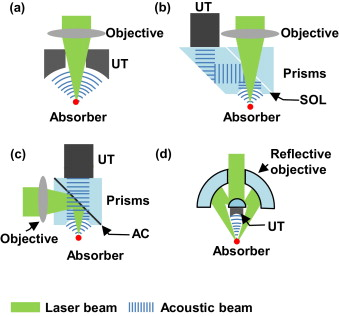
\includegraphics[width = 0.55\textwidth, height=0.3\textheight]{02_principles_of_photoacoustics/images/pamSetups.jpg}
	\caption{Typically used OR-PAM setups. In a) a hole is drilled into the Ultrasonic Transducer (UT), b) uses a silicon oil for refractive index matching (SOL) and therefore generates a optical transparent but acoustical reflective interface, c) is vise versa where the aluminum coating (AC) redirects the laser light and d) uses a reflective objective to focus the light onto the sample \cite{YAO201487}.}
	\label{fig:PAMsetup}
\end{figure}

There are several advantages and disadvantages to every setup.  For example in a), there are losses due to the hole, that have to be drilled into each ultrasonic transducer. In b) and c) the idea is to redirect either the acoustical or the optical pathway. This redirection goes at the expanse of working distance of the applicable objective and therefore the possible Numerical Aperture (NA). In version d) a high NA is possible, but there are losses due to the cable connection for the ultrasonic transducer in the middle. 

\subsubsection{OR-PAM setup}
\label{sec:ORPAMsetup}

The performed measurements were done with the setup shown in Figure \ref{fig:PAMsetup} b). The crucial factor for the choice were the commercial availability of all components used in the setup.\\
For positioning linear stages were used. In x-direction, a PI M-605.2DD controlled by a PI Mercury C-863  and in y-direction a Thorlabs Z825B controlled by a Thorlabs TDC001. The used ultrasonic transducer was an Olympus Panametrics V214-BB-RM with a center frequency of 50~MHz.\\
After the ultrasonic wave is converted into a voltage signal it gets amplified by two Minicircuit ZFL-500LN+ with about 20~$dB$ amplification each. The digitalization is done by a Spectrum M3i.4140-Exp measurement card. Furthermore, the data acquisition and system control is done by a LabVIEW program running on a PC. 

\begin{figure}[H]
	\centering
	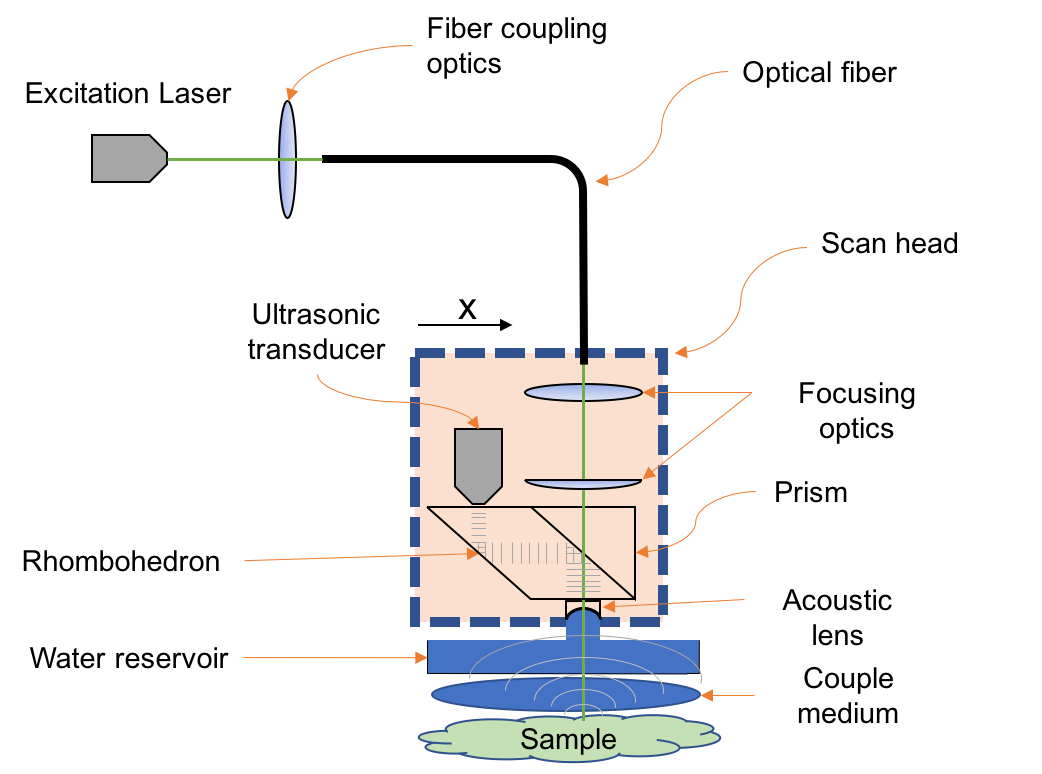
\includegraphics[width = 0.9\textwidth]{02_principles_of_photoacoustics/images/ORPAMsetup.png}
	\caption{Schematic view of the used OR-PAM setup.  }
	\label{fig:ORPAMsetup}
\end{figure}

If the scan head (area, surrounded by the dashed line) is in the right position, the x-direction stage triggers a Quantum Composer 9520 Delay Generator (DG). This device generates a trigger signal for a LCM-DTL-319QT (527 nm) Laser, the measurement card and an oscilloscope that tracks the laser power via a Thorlabs PM100A, with a S120VC photodiode. The laser light is brought to the setup by an optical fiber (Thorlabs P1-460B-FC singlemode, \o = 3.6~$\mu m$).\\
The optical section of the scan head consist of a lens to collimate the laser beam (f = 40~$mm$) and a lens that focuses the light onto the sample (f = 80~$mm$). Acoustically the scan head is coupled to the water reservoir by a water drop that stick at the acoustic lens (45-008 from Edmund Optics), that is glued centered, underneath the rhombohedron prism. The bottom side of the reservoir is made of an acoustical and optical transparent polymer membrane. The sample is acoustically coupled onto the membrane, that restrain the water via a coupling media. Therefore commonly a water droplet is used. \\
The generated ultrasonic wave travels back the optical path. After hitting the acoustic lens the spherical propagating wavefront gets transformed into a plane wave with mostly longitudinal components. The first reflection on the interface between rhombohedron and right-angel prism converts the major part into transversal wave components. In order to properly detected by a piezo electric ultrasonic transducer the signal has to be transformed back into a longitudinal wave, to avoid significant loss of signal strength and information. This is done by a second reflection at the interface (glass/air) on the left side of the rhombohedron prism \cite{Hu:11}. \\
As shown in figure \ref{fig:PAMsetup} b) an index matching liquid is applied to the interface between the rhombohedron and the prism. This ensures that the acoustical wave is deflected on the one hand and the laser beam passes without reflection losses on the other hand. 

\subsubsection{Acoustical runtime considerations}

The time, the ultrasonic wave takes to generate a voltage signal, is important to distinguish between the source signal and the setup reflections. As both reflections come along with mode transformations and therefore differing propagation directions, a detailed investigation were done.\\
In figure \ref{fig:acousticalPath} a closer look onto the setup, described in figure \ref{fig:ORPAMsetup}, is shown. Additionally the estimated acoustic paths, \textit{Path A} and \textit{Path B}, are added.

\begin{figure}[H]
	\centering
	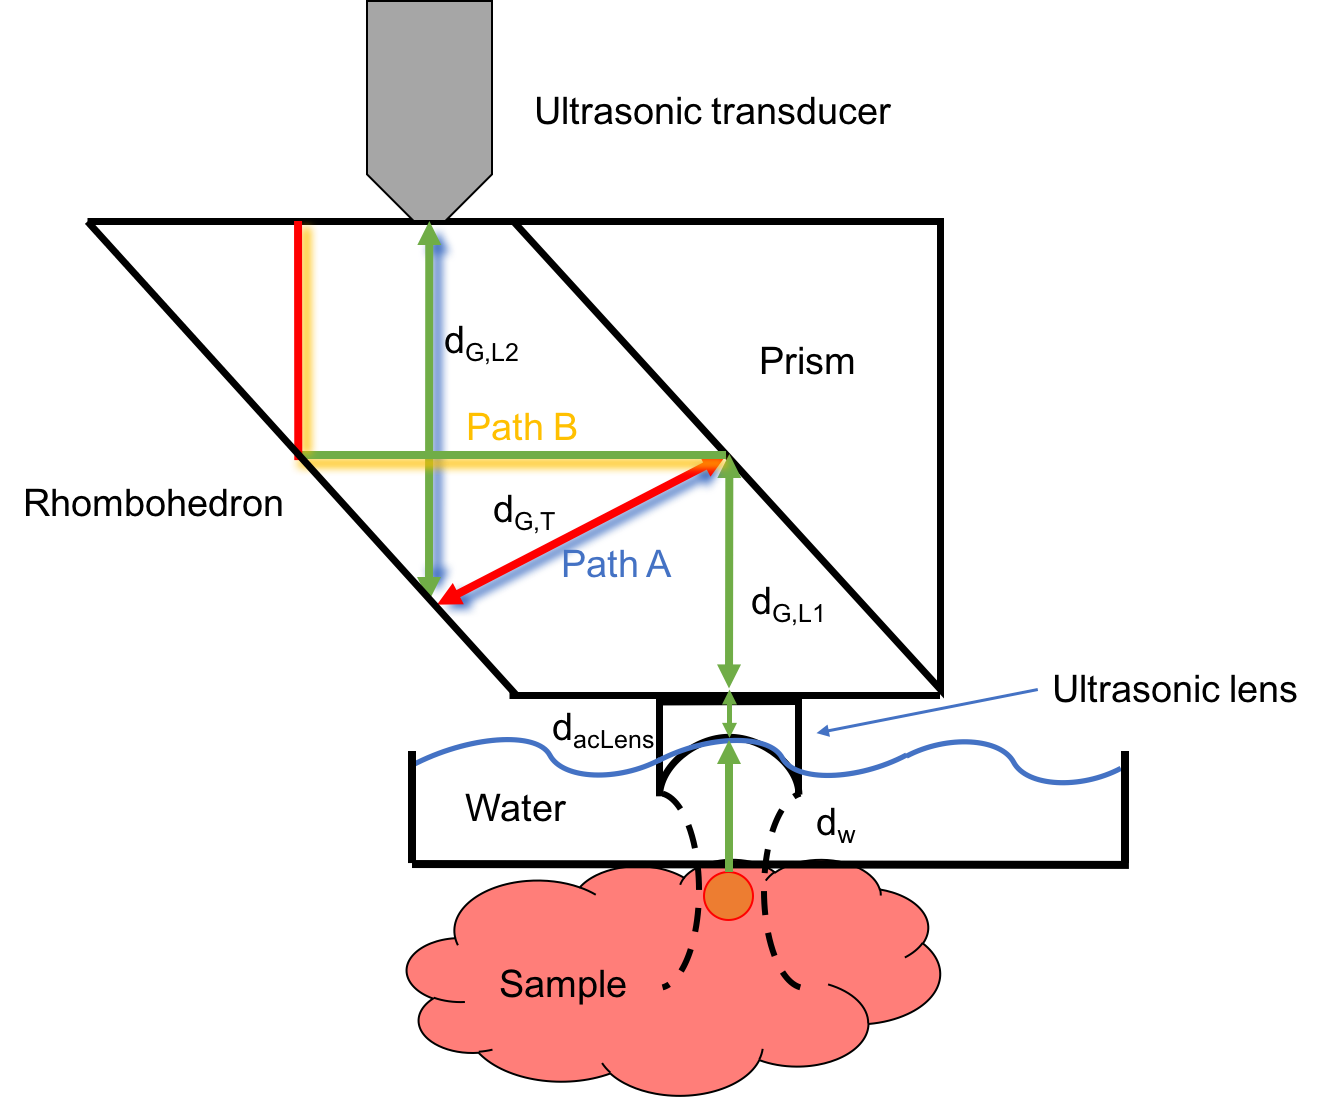
\includegraphics[height = 0.35\textheight, width = 0.6\textwidth]{02_principles_of_photoacoustics/images/ultrasonicPath.png}
	\caption{Zoomed view of figure \ref{fig:ORPAMsetup}. Here the paths taken by the ultrasonic wave are added. The green lines mark longitudinal wave components and the red lines the transversal.}
	\label{fig:acousticalPath}
\end{figure}

The generated ultrasonic wave is a spherical longitudinal wave, which gets transformed into a plane wave by the acoustical lens. As shown in figure \ref{fig:acousticalPath} the longitudinal wave gets mode converted on the right (rhombohedron-prism interface) and the left side (rhombohedron-air interface) of the rhombohedron. The first reflection splits the incident beam into a acoustical \textit{Path A} and \textit{Path B}. Due to the property, of the ultrasonic transducer, to only detect longitudinal modes, the investigated path were \textit{Path A}.\\
For the assumption, that the ultrasonic source object is in the focal plane and the interface between the acoustical lens and the rhombohedron has no impact, the acoustical travel time is 

\begin{equation}
t_{trav} = \frac{d_w}{c_w} + \frac{d_{G,L1}+d_{G,L2}+d_{acLens}}{c_{G,L}} + \frac{d_{G,T}}{c_{G,T}} + t_D
\label{eq:travTime}
\end{equation}
\\
where $d_w$ is the distance the wave travels in water, $d_{G,L1}$ and $d_{G,L2}$ are the longitudinal travel distances in glass and $d_{G,T}$ is the transversal one. The material for the acoustical lens is equal to the rhombohedron material (N-BK7), therefore the speed of sound is the same as for the longitudinal components in glass $c_{G,L}$. Furthermore, the ultrasonic transducer has a delaytime $t_D$. \\
In table \ref{tab:matSpecs} the speed of sound values for the appearing materials are listed.

\begin{table}[H]
	\centering
	\caption{Speed of sound values for N-BK7 and water.}
	\begin{tabular}{| m{2.2cm} | c | c |}
		\hline
		&$c_{longitudinal}$&$c_{transversal}$\\ \hline
		\centering N-BK7 \cite{data:BK7}&6048~$m/s$ &3680~$m/s$\\ \hline
		\centering Water \cite{Haynes:physicalProperties} &1483~$m/s$& - \\ \hline
	\end{tabular}
	\label{tab:matSpecs}
\end{table}

To determine $d_{G,T}$ and $d_{G,L2}$, the behavior of acoustical waves on interfaces is examined. Mechanical waves basically follow Snell's just as optical waves do. \\
In solids a incident longitudinal pressure wave $P_i$, shown in figure \ref{fig:acousticInterface}, transforms into a reflected longitudinal ($P_{P,r}$) respectively transversal part ($P_{T,r}$) and a transmitted longitudinal ($P_{P,t}$) respectively transversal part ($P_{T,t}$), on an interface.

\begin{figure}[H]
	\centering
	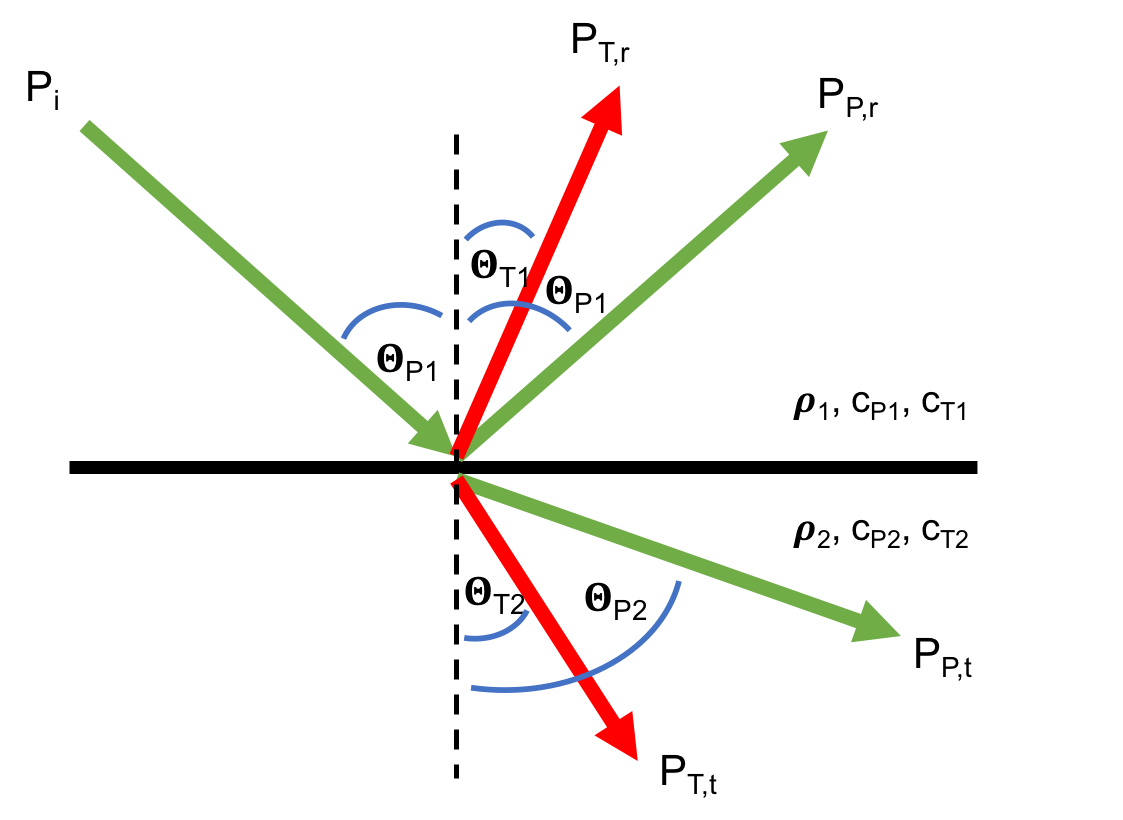
\includegraphics[height = 0.33\textheight, width = 0.58\textwidth]{02_principles_of_photoacoustics/images/acousticInterface.png}
	\caption{Behavior of acoustical waves on interfaces. The longitudinal and transversal wave components are marked with green and red lines.}
	\label{fig:acousticInterface}
\end{figure}

Therefore Snell's law is 

\begin{equation}
	k_{Pi} \sin(\theta_{Pi}) = k_{P_{T,r}} \sin(\theta_{P_{T,r}}) = k_{P_{P,r}} \sin(\theta_{P_{P,r}}) = k_{P_{T,t}} \sin(\theta_{P_{T,t}}) = k_{P_{P,t}} \sin(\theta_{P_{P,t}})
\end{equation}
\\
where k is the wave vector $k_i = \frac{2 \pi f}{c_i}$. \\
The modified lensmaker equation gives the focal length of the acoustical lens and therefore the travel distance for the pressure wave in water \cite{GraflMonika2015Pm}.
\begin{equation}
f_{ac} = d_w = - R \cdot \frac{1}{\frac{c_w}{c_{N-BK7}}-1} = 8.21~mm
\end{equation}
\\
The value for $R$ = 6.2~$mm$ and for $d_{acLens}$ = 1.5~$mm$ (center thickness value) were taken from the 45-008 datasheet \cite{data:45008}.\\
The delaytime of the ultrasonic transducer is 2.15~$\mu s$. The values for $d_{G,T}$ (11.75~$mm$), $d_{G,L1}$ (7.5~$mm$) and $d_{G,L2}$ (11.42~$mm$) are solved by geometrical optics. \\
Inserting into formula \ref{eq:travTime} follows for the acoustical travel time $t_{trav}$ = 14.26~$\mu s$.\\
Signals, which are in the range of $t_{trav}$,  are considered to be generated at the acoustical focal plane.
\pagebreak
\subsubsection{Data acquisition (DAQ) in PAM}
\label{sec:DAQ}

In order to record an image in OR-PAM, a certain sequence have to be executed. \\
At first a field size is defined in the user interface. For example in Figure \ref{fig:scanProcess} a field of view 300 x 300 ($N_x$ x $N_y$) points and a  stepsize of 20~$\mu m$ in both directions are chosen. 

\begin{figure}[H]
	\centering
	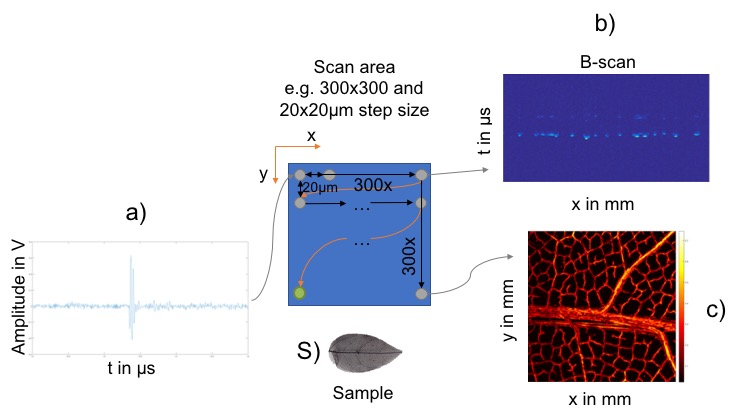
\includegraphics[width = 0.9\textwidth]{02_principles_of_photoacoustics/images/scanProcess.jpg}
	\caption{Illustrated procedure of a scan process. Sample is the black plastic leaf S). a) shows a typical photoacoustic A-scan signal, b) a B-scan image and c) a generated C-scan image, where the maximum of each recorded A-scan is taken.}
	\label{fig:scanProcess}
\end{figure}

In \ref{fig:scanProcess} a) a typical photoacoustic signal is shown, that is called A-scan. At every point in the scan area such a A-scan signal is recorded. As the scan head moves over the sample, every 20~$\mu m$ a detection point is taken. After 300 recorded points in x-direction the scan head moves into the next line. \\
If the 300 A-scan signals are drawn together, a B-scan as shown in \ref{fig:scanProcess} b) is created. A B-scan is termed to be a cut through the sample. The x-coordinate gives the length and the y-coordinate the time-depth (recorded sequence) of the cut.\\
After 300 lines are scanned, a three dimensional cube is created with the size of 

\begin{equation}
	V_{PAcube} = N_x \cdot \Delta x \cdot N_y \cdot \Delta y \cdot t \cdot c_s
\end{equation}
\\
where $t$ is the recorded time interval and $c_s$ the average speed of sound between origin of the ultrasonic wave and the transducer. Based on that several data analysis operations can be executed. For example the maximum amplitude of each photoacoustic amplitude (PA) track, shown in Figure \ref{fig:scanProcess} a), can be extracted and displayed, shown in Figure \ref{fig:scanProcess} c).\\
Furthermore, a topological mapping of the sample is possible due to the runtime information of the ultrasonic signal. This is shown in section \ref{sec:topoPAI}. 

\subsubsection{Hilbert transformation in PAM}

The Hilbert transformation (HT) is an integral transformation equal to the Fourier transformation. In signal processing theory it is used to assign an analytical signal $\hat{x}(t)$ to a real signal $x(t)$. 

\begin{equation}
\hat{x}(t)= x(t) + j \mathcal{H}\{x(t)\}
\end{equation}
\\
An analytical signal is a complex function and has no negative frequencies in its spectrum and is therefore causal. This leads to the property that real and imaginary parts of $\hat{x}(t)$ can be converted into each other, as follows

\begin{equation}
	Re\{\hat{x}(t)\} = - \mathcal{H}\{Im\{\hat{x}(t)\}\}
\end{equation}
\begin{equation}
	Im\{\hat{x}(t)\} =  \mathcal{H}\{Re\{\hat{x}(t)\}\}
\end{equation}
\\
For example, $x(t) = \cos(\omega_0 t)$. The corresponding Hilbert transformed is $\mathcal{H}\{x(t)\} = \sin(\omega_0 t)$ and therefore the analytical signal

\begin{equation}
\hat{x}(t) =  \cos(\omega_0 t) + j \sin(\omega_0 t) 
\end{equation}
\\
the absolute value is $r = \sqrt{\cos(\omega_0 t)^2 +  \sin(\omega_0 t)^2} = 1$ and also the complex envelope of $x(t)$. In figure \ref{fig:PAhilbertSim} this principle were applied to a PA signal \cite{book:girodSystemtheorie}.  

\begin{figure}[H]
	\centering		
	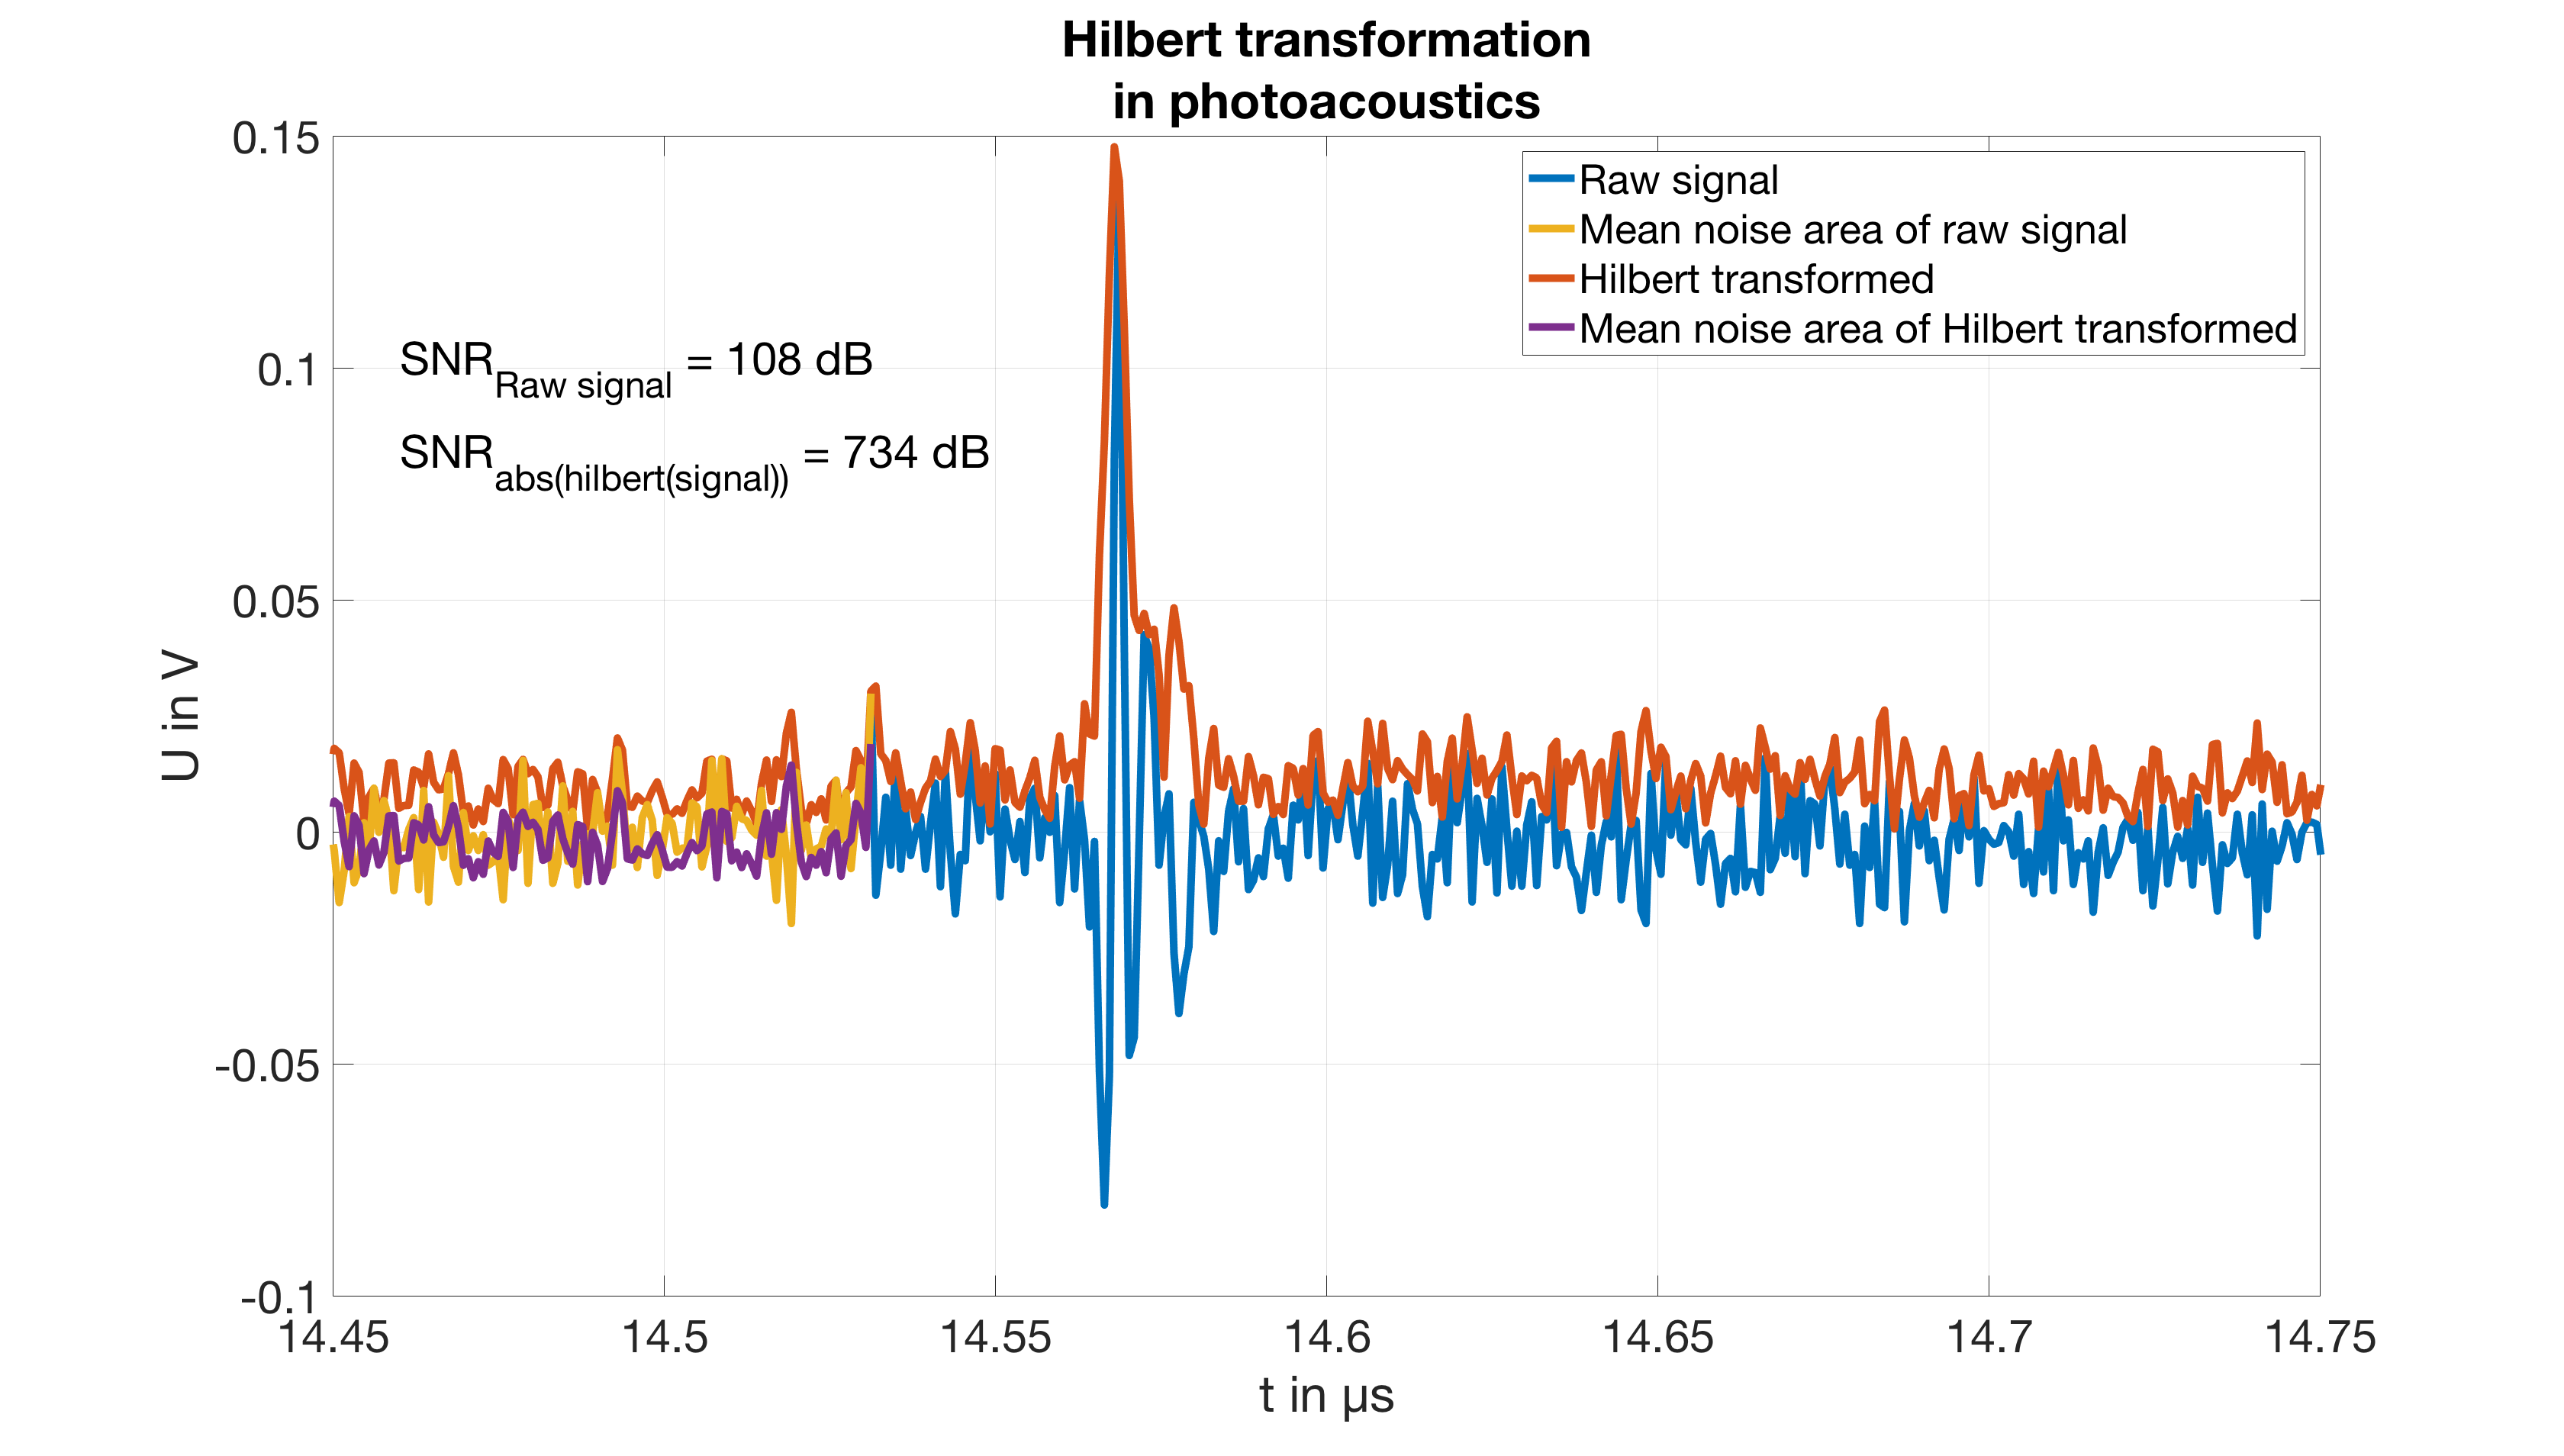
\includegraphics[width = \textwidth]{02_principles_of_photoacoustics/images/measHilbertPA.png}
	\caption{The blue line is the measured PA and its Hilbert transformation in orange. For the signal to noise ratio (SNR) the maximum amplitude of the signals and the mean noise displayed in yellow for the raw signal and purple for the Hilbert transformed. Furthermore, the constant component of the Hilbert transformed were subtracted. }
	\label{fig:PAhilbertSim}
\end{figure}

The blue line is the PA signal and the orange line is the absolute value of its Hilbert transformed. Inside the plot the SNR values for both are shown. For the Hilbert transformed line the value is about seven times higher than the original one.\\
Therefore the HT is a helpful method to suppress noise. The drawback is that the full width at half maximum (FWHM) broadens. As the axial resolution of OR-PAM is determined by the frequency bandwidth of the detecting ultrasonic transducer and thus to the FWHM of the detected signal, the HT reduces the resolution \cite{Ma:GRPAMinVivo}.\\ 
In figure \ref{fig:BsacanHilbert} the difference between a normal B-scan a) and a B-scan, where every detected sequence were Hilbert transformed b), is shown.

\begin{figure}[H]
	a)
	\begin{minipage}{\textwidth}		
		\centering
		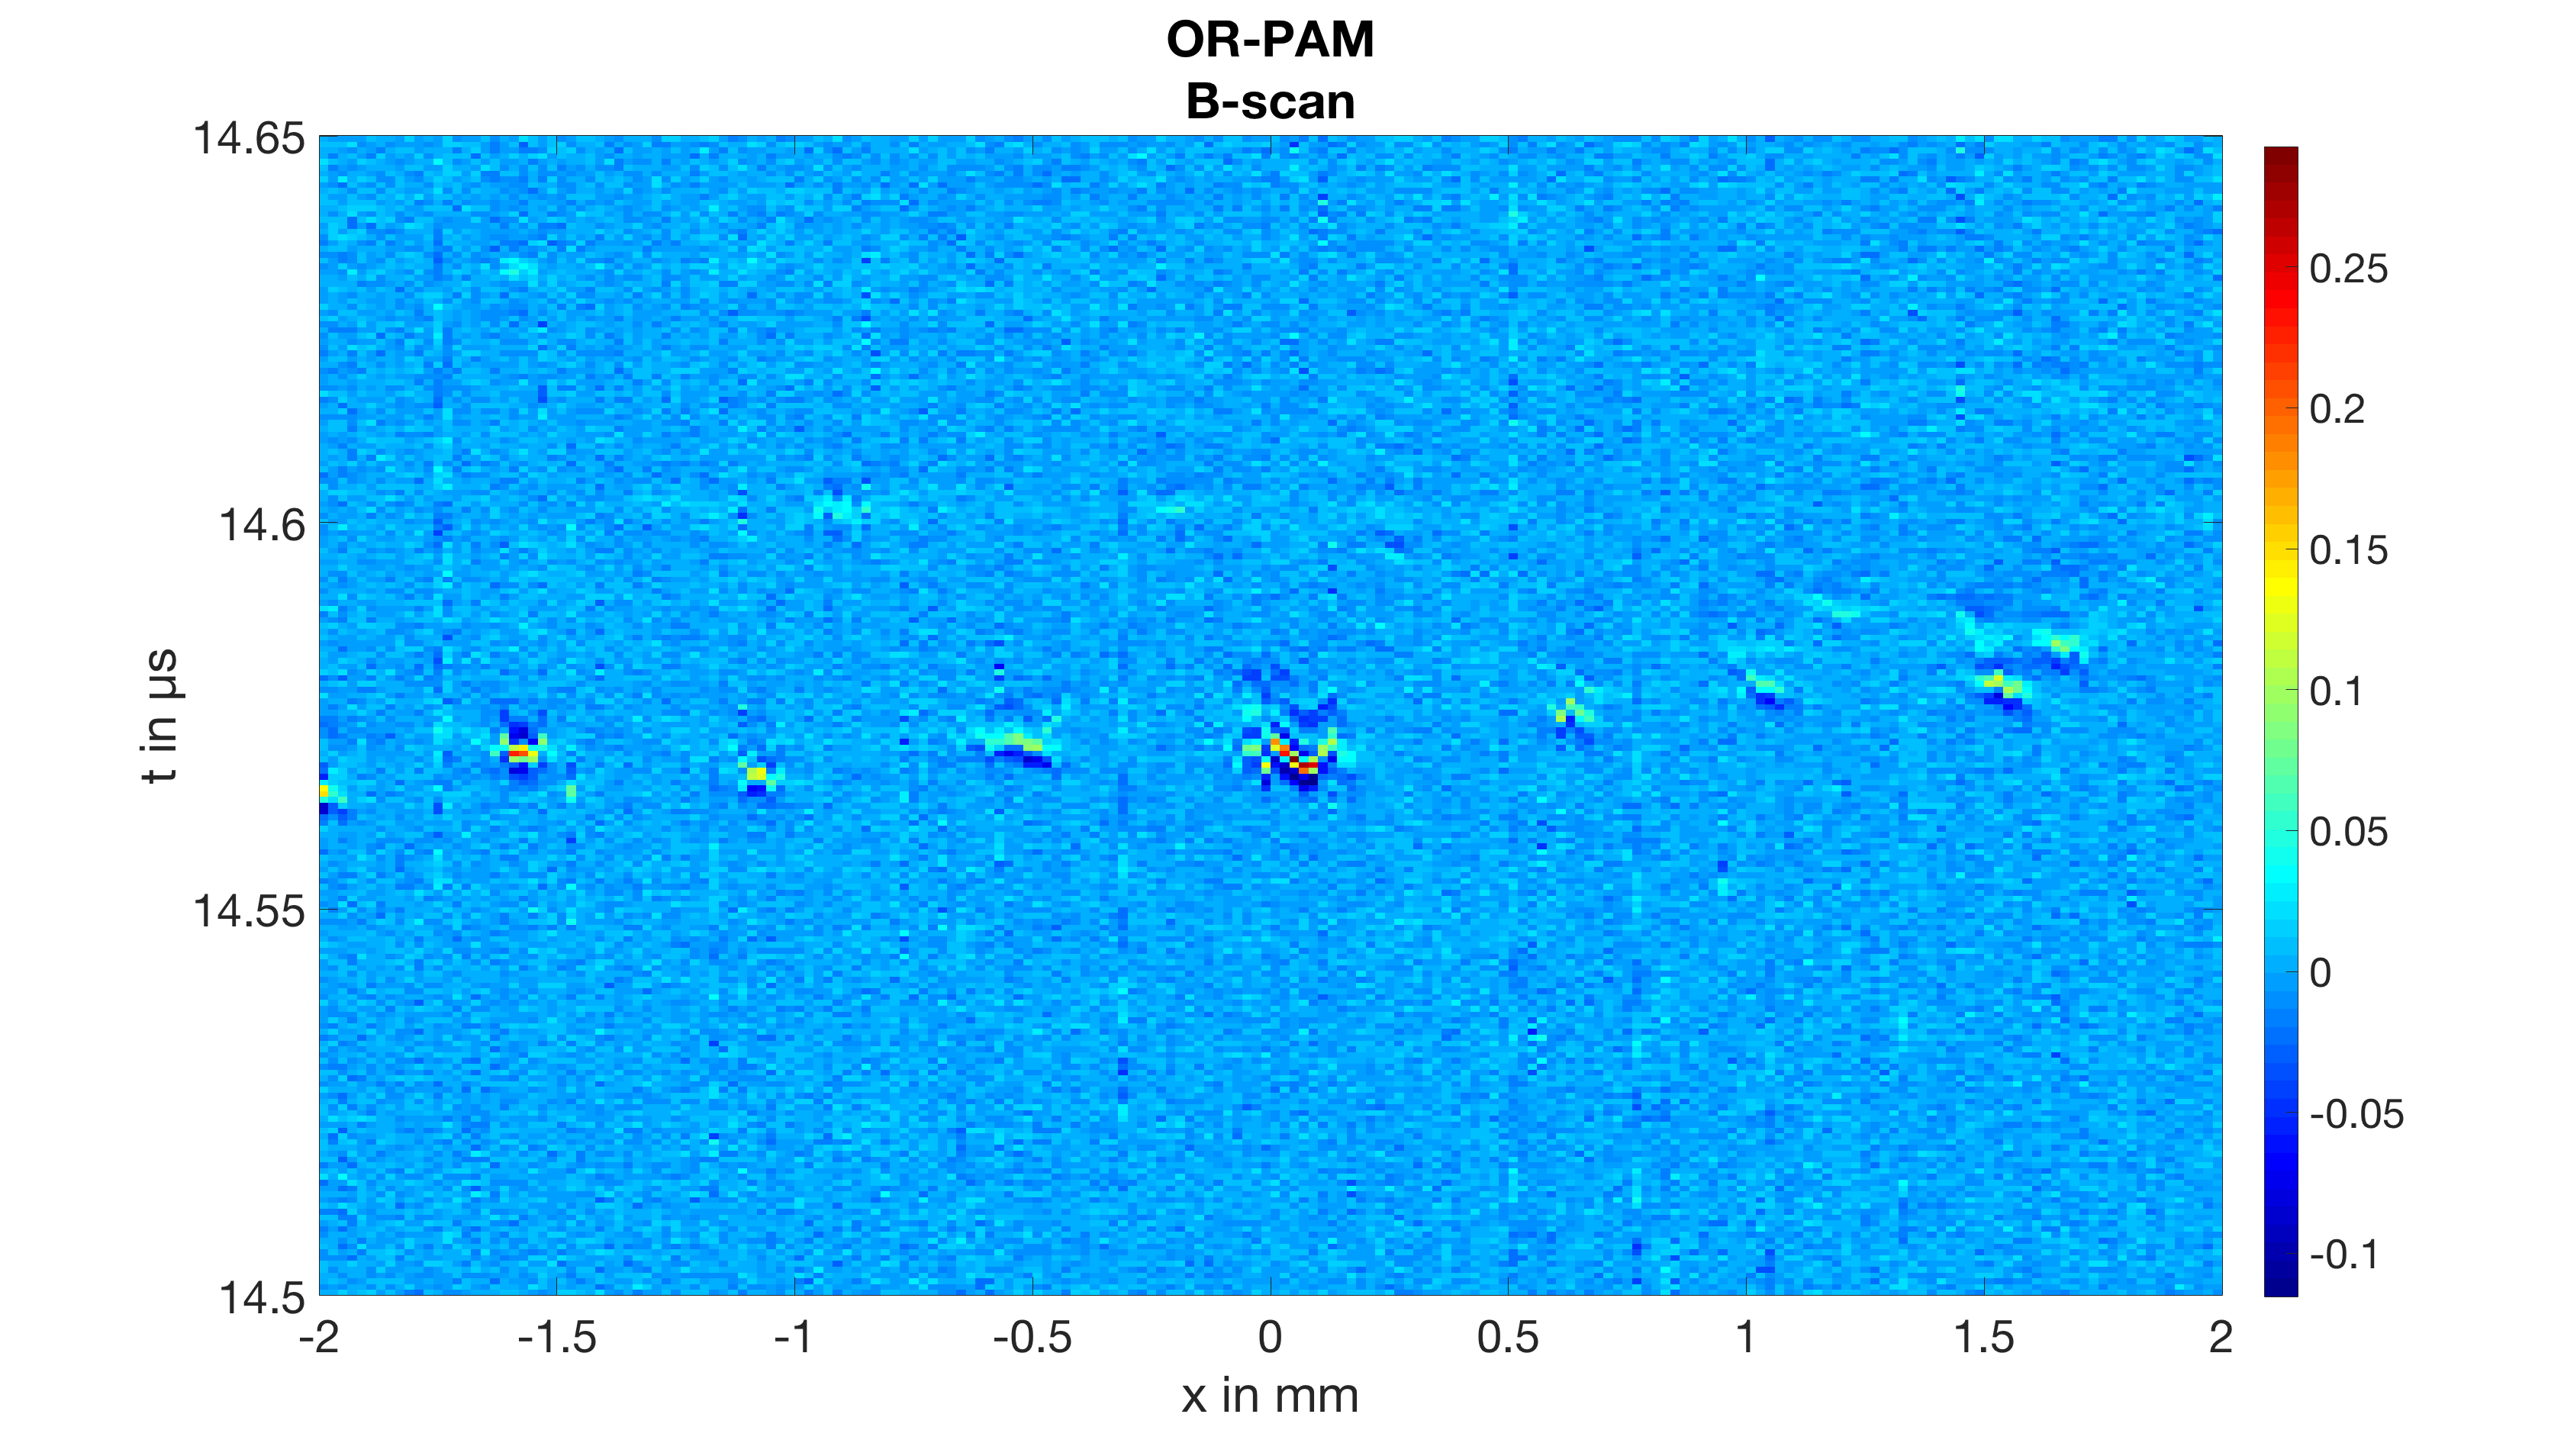
\includegraphics[width = \textwidth]{02_principles_of_photoacoustics/images/Bscan.png}
	\end{minipage}
	b)
	\begin{minipage}{\textwidth}		
		\centering
		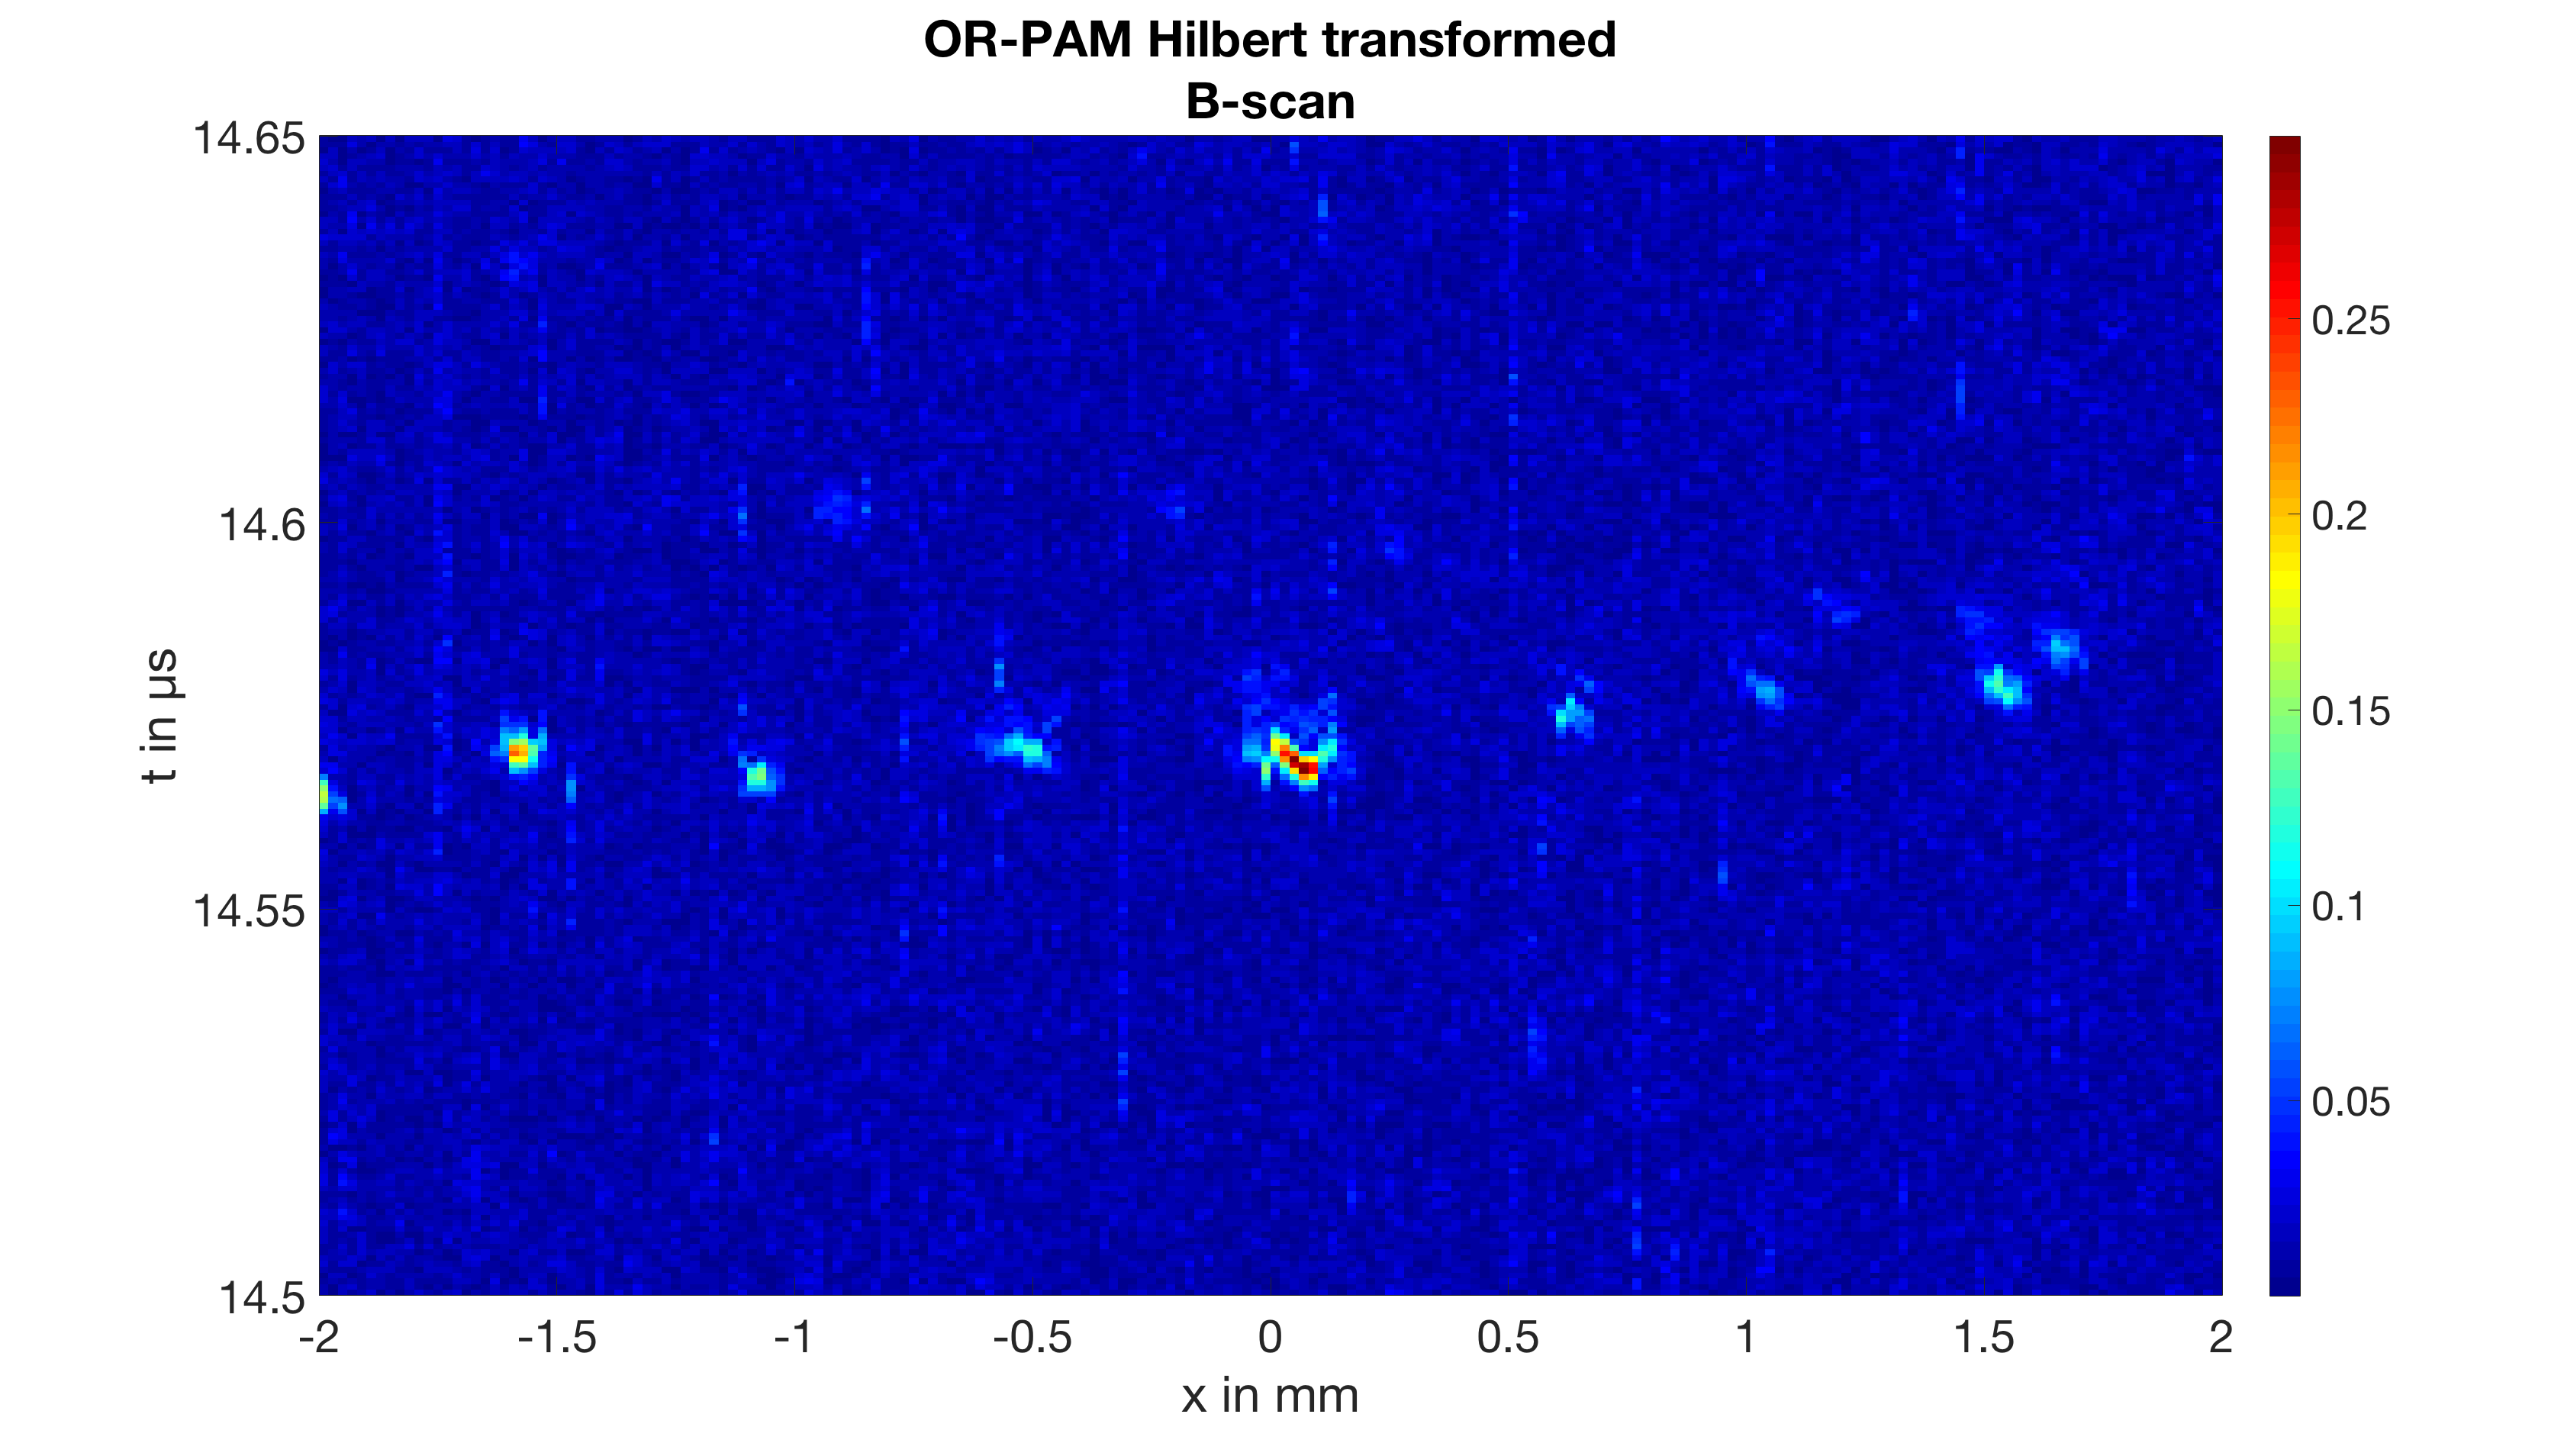
\includegraphics[width = \textwidth]{02_principles_of_photoacoustics/images/BscanHilbert.png}
	\end{minipage}	
	\caption{In a) a normal B-scan is shown and in b) its absolute value of the Hilbert transformed.}
	\label{fig:BsacanHilbert}
\end{figure}

In b) the effect is clearly visible, the SNR is observable higher than in a). \\
Therefore the HT is a efficient way to reduce noise in PAM images. 



\section{Grueneisen relaxation photoacoustic microscopy (GR-PAM) theory}

In this section the Grueneisen effect is characterized theoretical and the application to microscopy is shown. Furthermore, the influence of varying laser wavelengths to GR-PAM is studied and a method to determine the absorption coefficient $\mu_a$ is presented. 

\subsection{The Grueneisen effect}
\label{sec:GReffect}
The initial pressure rise is defined by $p = \Gamma \mu_a F$ as discussed in chapter \ref{sec:photoeffect}. There the Grueneisen parameter $\Gamma$ is given by

\begin{equation}
\Gamma = \frac{\beta(T) \cdot c_s^2(T)}{C_p(T)}
\label{eq:gamma(T)}
\end{equation}

$\beta$ is the thermal expansion coefficient, $c_s$ is the speed of sound and $C_p$ is the specific heat capacity at constant pressure. All components of $\Gamma$ are temperature dependent. The change of the PA in terms of temperature is called Grueneisen effect. \\
The main contribution to this change comes from $\beta$. It rises at about 97~\% by a temperature change from 20~$^\circ$C to 40~$^\circ$C. There the contribution from $c_s$ and $C_p$ is less than 4~\% and 1~\% \cite{waterproperties, Tian:dualPulse}. 
This leads to the conclusion, that the Grueneisen parameter primarily depends on $\beta$. \\
Figure \ref{fig:GeffectPaper} shows the dependence of pressure amplitude from temperature. The measured amplitudes are normalized against the pressure amplitude at 26~$^\circ$C. 

\begin{figure}[H]
	\centering
	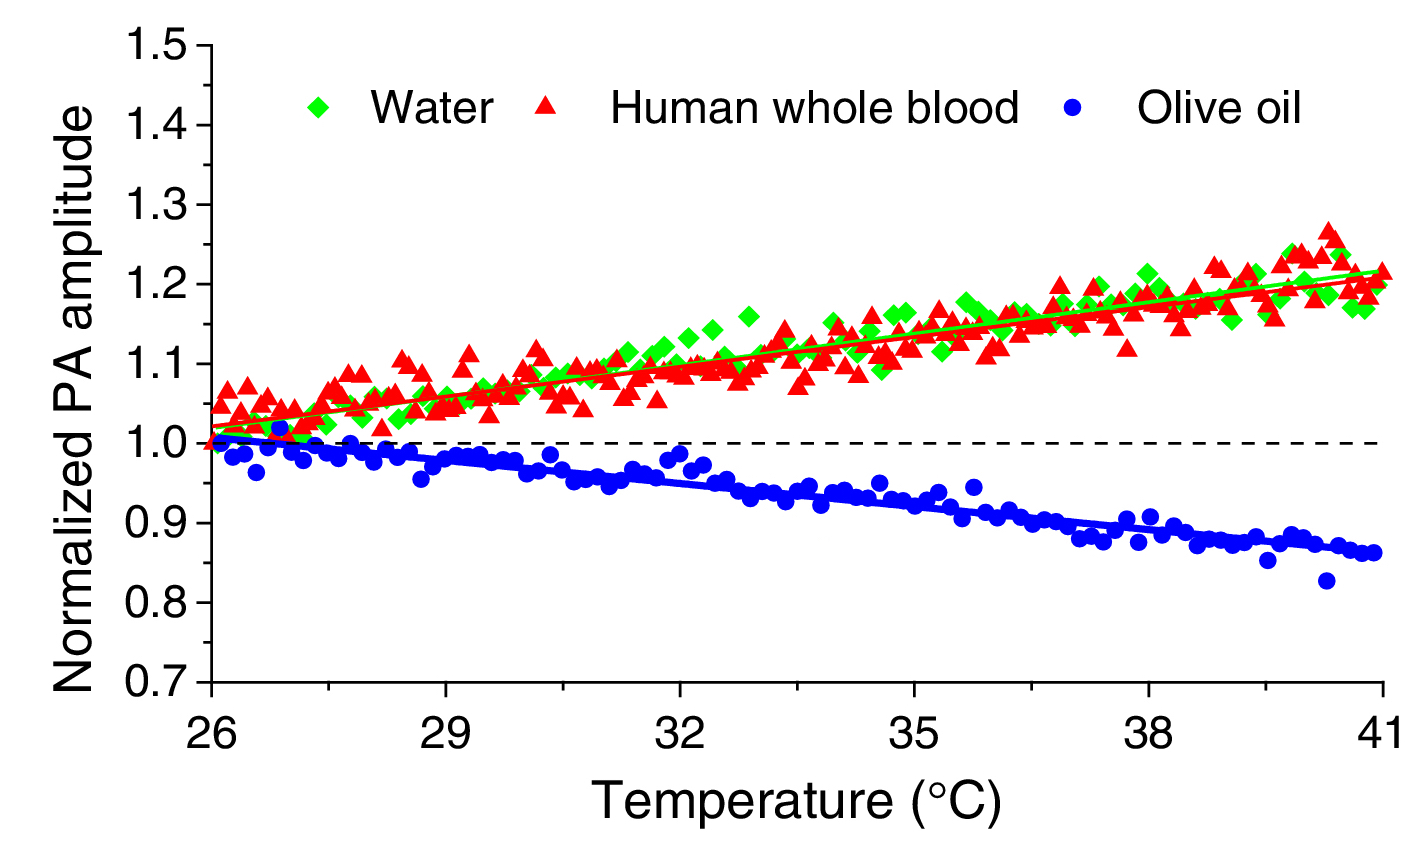
\includegraphics[width = 0.75\textwidth, height=0.3\textheight]{03_GR-PAM_theory/images/GeffectPaper.jpeg}
	\caption{Normalized pressure amplitude in dependence of temperature for water, human whole blood and olive oil. \cite{Tian:15}}
	\label{fig:GeffectPaper}
\end{figure}

It can be seen that the amplitude of water and blood rises while the one for olive oil decreases. Therefore the Grueneisen effect can be used to establish a contrast between thermal differing properties of the sample compounds. For example blood and fatty tissue can be separated \cite{Tian:15}. Another advantage is that most physical parameters of tissue have a strong temperature dependence \cite{Jacques:opticalPropsBiotissue}. 

\subsection{Dual pulse technique}
\label{sec:dualPulseTechnique}

In order to make the Grueneisen effect usable for microscopy, a significant temperature rise has to be employed into the area of interest. This can be done with a two laser pulse process sketched in figure \ref{fig:doublePulse}.\\
The laser pulses have to be in a nanosecond range. The first one at time $t_1$, called heating pulse, applies a significant temperature rise into the area of interest. The second one, called detecting pulse, is delivered to the sample with a submicrosecond delay and excites a second pressure wave, but this one is modified due to the Grueneisen effect. 

\begin{figure}[H]
	\centering
	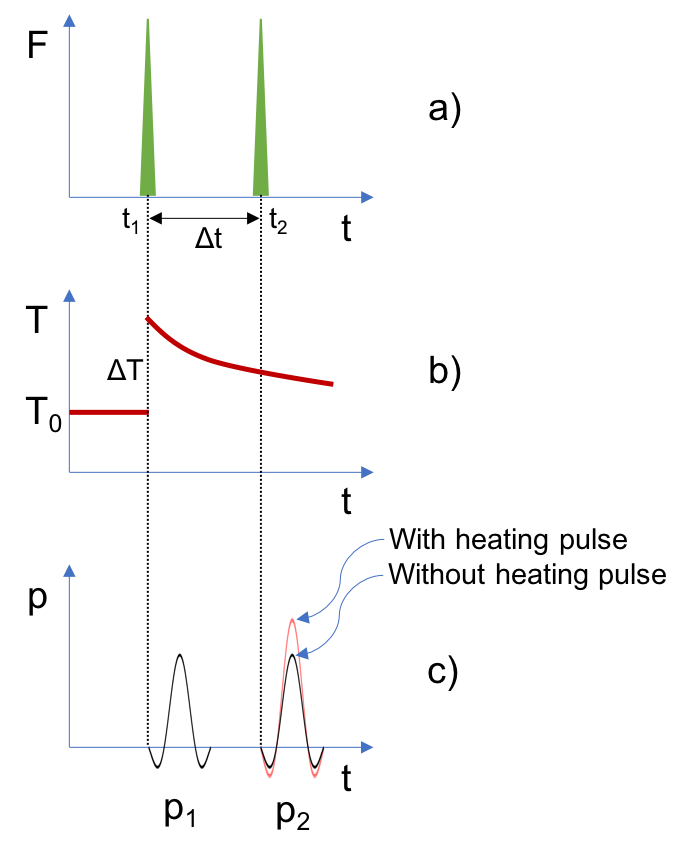
\includegraphics[width = 0.5\textwidth]{03_GR-PAM_theory/images/dualPulse.png}
	\caption{Signal generation sequence for GR-PAM with G $>0$.}
	\label{fig:doublePulse}
\end{figure}

The initial pressure rise p$_1$ is identical to equation \ref{eq:p_0}, with equilibrium temperature $T_0$ and $\Gamma_0$. For the following considerations a heat conversion coefficient $\eta_{th}$ were added, this coefficient pools all side effects and acts as a correction factor

\begin{equation}
	p_1 = \Gamma \eta_{th} \mu_a F
\end{equation}
\\
If the second laser pulse hit the sample before the temperature has reached the equilibrium state again, a pressure rise p$_2$ is formed given by

\begin{equation}
	p_2 = \Gamma(T_0 + \Delta T, \Delta t) \eta_{th} \mu_a F_2
	\label{eq:grPA2}
\end{equation} 

\begin{equation}
\Gamma(T_0 + \Delta T, \Delta t) = \Gamma_0 + G \cdot \Delta T \cdot \tau(\Delta t)
\end{equation} 
\begin{equation}
\Delta T = \eta_{th} \mu_a F_1
\end{equation} 
\\
there G is a coefficient that relates to the change of the Grueneisen parameter and $\tau$ a relaxation function (compare Figure \ref{fig:doublePulse} b) \cite{Ma:GRPAMinVivo,Tian:15}. As seen in Figure \ref{fig:GeffectPaper} the change of the Grueneisen parameter can either be positive or negative and thus G can be. Therefore G in Figure \ref{fig:doublePulse} is positive, this results in a higher amplitude p$_2$ than without heating. In order to make the difference visible, p$_1$ gets subtracted from p$_2$. 

\begin{equation}
	\Delta p = p_2 - p_1 = G \eta_{th}^2 \mu_a^2 F^2
	\label{deltaP}
\end{equation}
\\
This equation is only valid if F$_1$ = F$_2$. Otherwise additional terms emerge. It can be seen, $\Delta$p and therefore G depend quadratically on the fluence. This makes the Grueneisen effect a non-linear effect.\\

\subsubsection{Influence of laser-wavelength differences to GR-PAM}

In Figure \ref{fig:doublePulse} has to be considered that both pulses have the same wavelength. But systems can vary from this ideal configuration. Differing heating volumes for heating (V$_1$, $\lambda_1$) and detecting (V$_2$, $\lambda_2$) pulse are a consequence. Furthermore, a different absorption coefficient can be valid. Therefore three cases can be deduced\\

\begin{itemize}
\centering
\item[1) ] $\lambda_1 = \lambda_2 ;\, \mu_a(\lambda_1) = \mu_a(\lambda_2) ;\, \delta_1 = \delta_2 \, and\, V_1 = V_2$
\item[2) ] $\lambda_1 \neq \lambda_2 ;\, \mu_a(\lambda_1) < \mu_a(\lambda_2) ;\, \delta_1 > \delta_2 \, and\, V_1 \supset V_2$
\item[3) ] $\lambda_1 \neq \lambda_2 ;\, \mu_a(\lambda_1) > \mu_a(\lambda_2) ;\, \delta_1 < \delta_2 \, and\, V_1 \subset V_2$
\end{itemize}

Case 1) is the ideal case. Both pulses have the same wavelength and thus the same $\mu_a$. Therefore penetration depth equals heating volume. In 2) the detection volume is embedded into the heating volume. Here the non-linear effect is higher than in case 1). Case 3) is vice versa, the detection volume is bigger and therefore the effect smaller \cite{Tian:dualPulse}.

\subsubsection{Measurement  of the absorption coefficient $\mu_a$}

In order to get to know the absorption coefficient of liquids the setup shown in figure \ref{fig:mu_aSetup} were built. \\
A pulsed laser were coupled into a optical fiber to deliver the light to the setup. The laser-wavelength have to be tunable, to perform the measurement over the desired wavelength range.  

\begin{figure}[H]
	\centering
	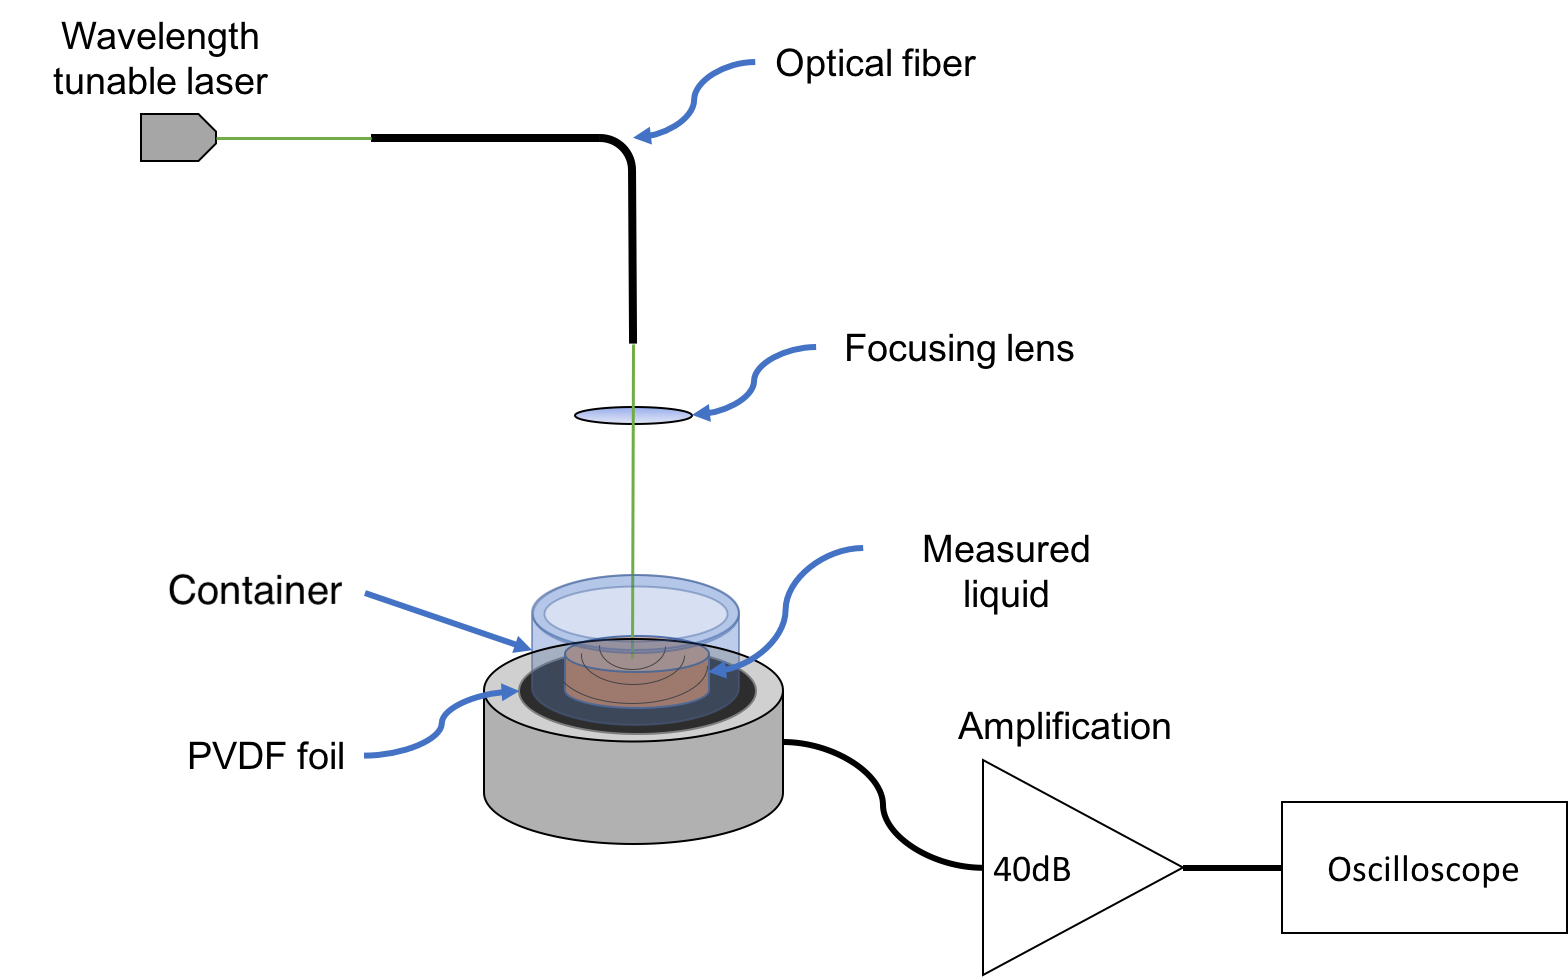
\includegraphics[width = \textwidth]{03_GR-PAM_theory/images/mu_aSetup.jpg}
	\caption{Measuring setup to determine the absorption coefficient.}
	\label{fig:mu_aSetup}
\end{figure}

In order to illuminate a certain area of the absorbing liquid, a bi-convex lens were used. The typical used liquid height is 5~$mm$. However, it has to be considered that liquids which have a high acoustic damping should have a lower level in order to get a decent signal. The container were sealed at the bottom with a thin polymer membrane to couple the soundwave with a minimum loss to the PVDF foil, which were placed on top of a metal housing. PVDF is a polymer with piezo-electric properties and therefore capable to detect ultrasonic waves. The foil generates a voltage signal, which is amplified by 40~$dB$ and displayed on an oscilloscope. The pressure rise can be written as 

\begin{equation}
p(t) = p_0 \cdot exp(-\mu_a(\delta-c_s t))
\end{equation}  
\\
where $p_0$ is the initial pressure rise (formula \ref{eq:p_0}) and $\delta$ the penetration depth (which is neglected for the fit) \cite{demtroder:ExPhysik}. 

\begin{figure}[H]
	a)
	\begin{minipage}{0.5\textwidth}		
		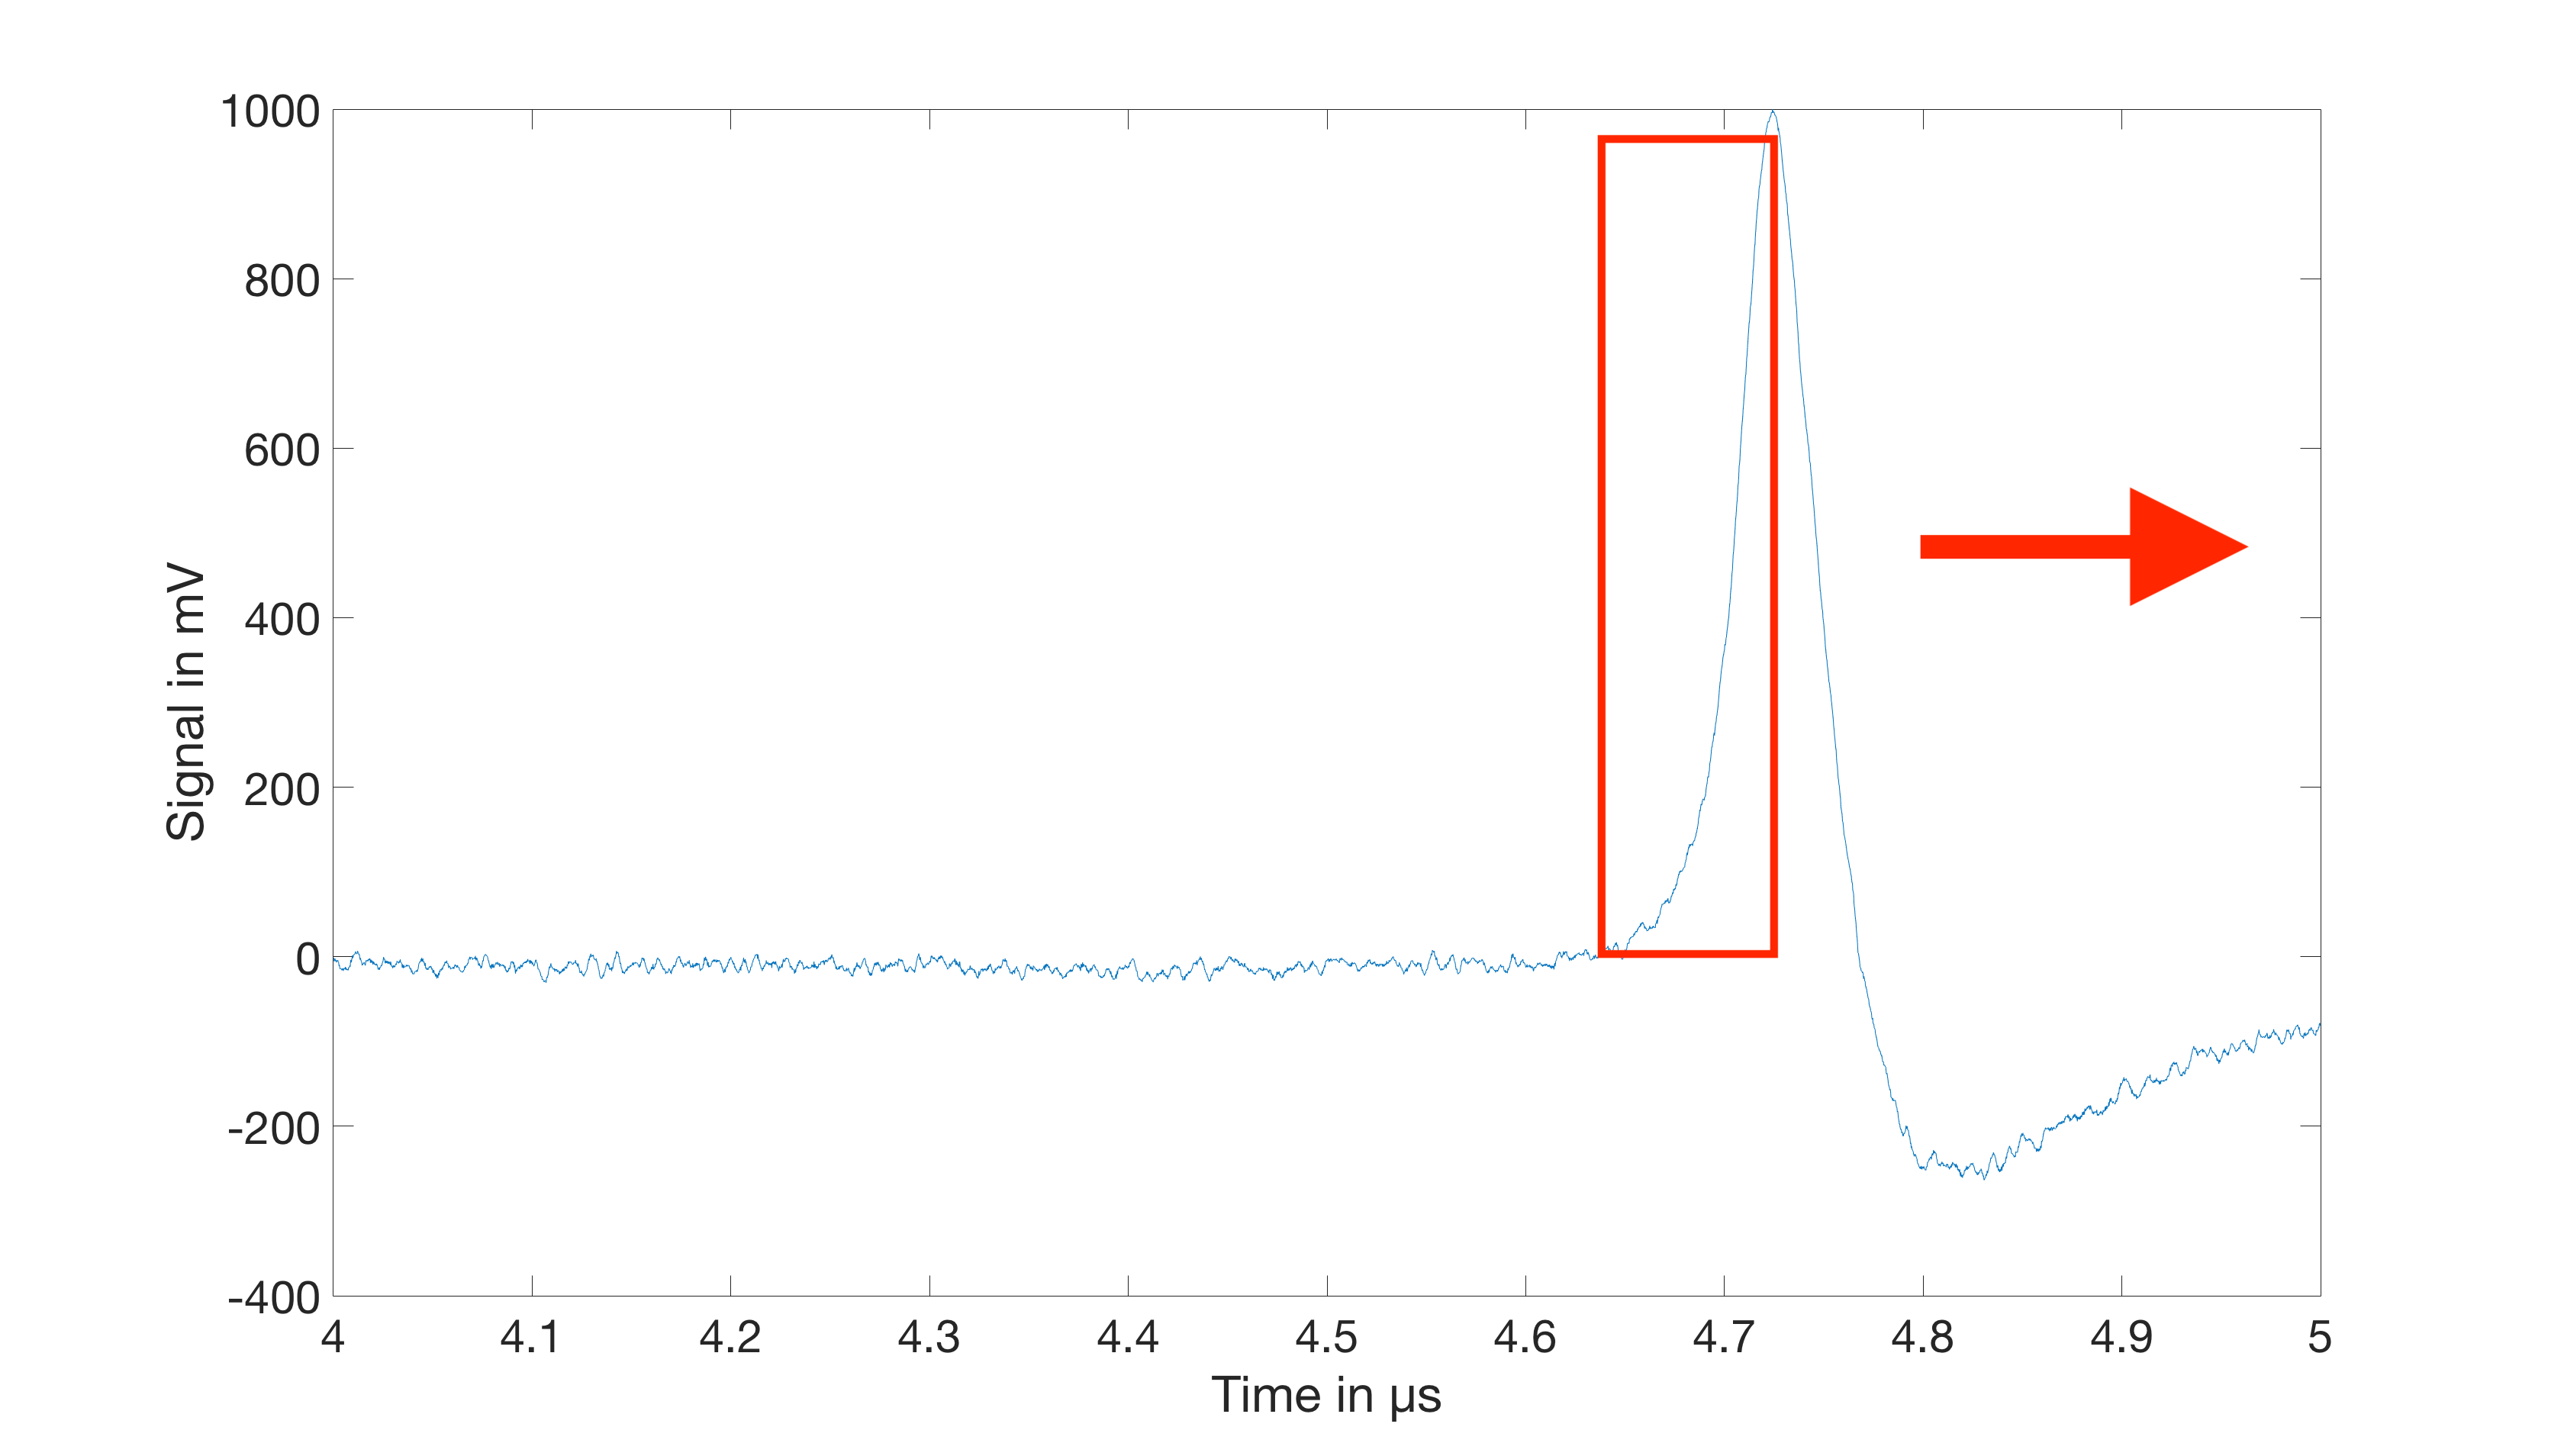
\includegraphics[width = \textwidth, height=0.25\textheight]{03_GR-PAM_theory/images/mu_aSig.png}
	\end{minipage}
	b)
	\begin{minipage}{0.5\textwidth}		
		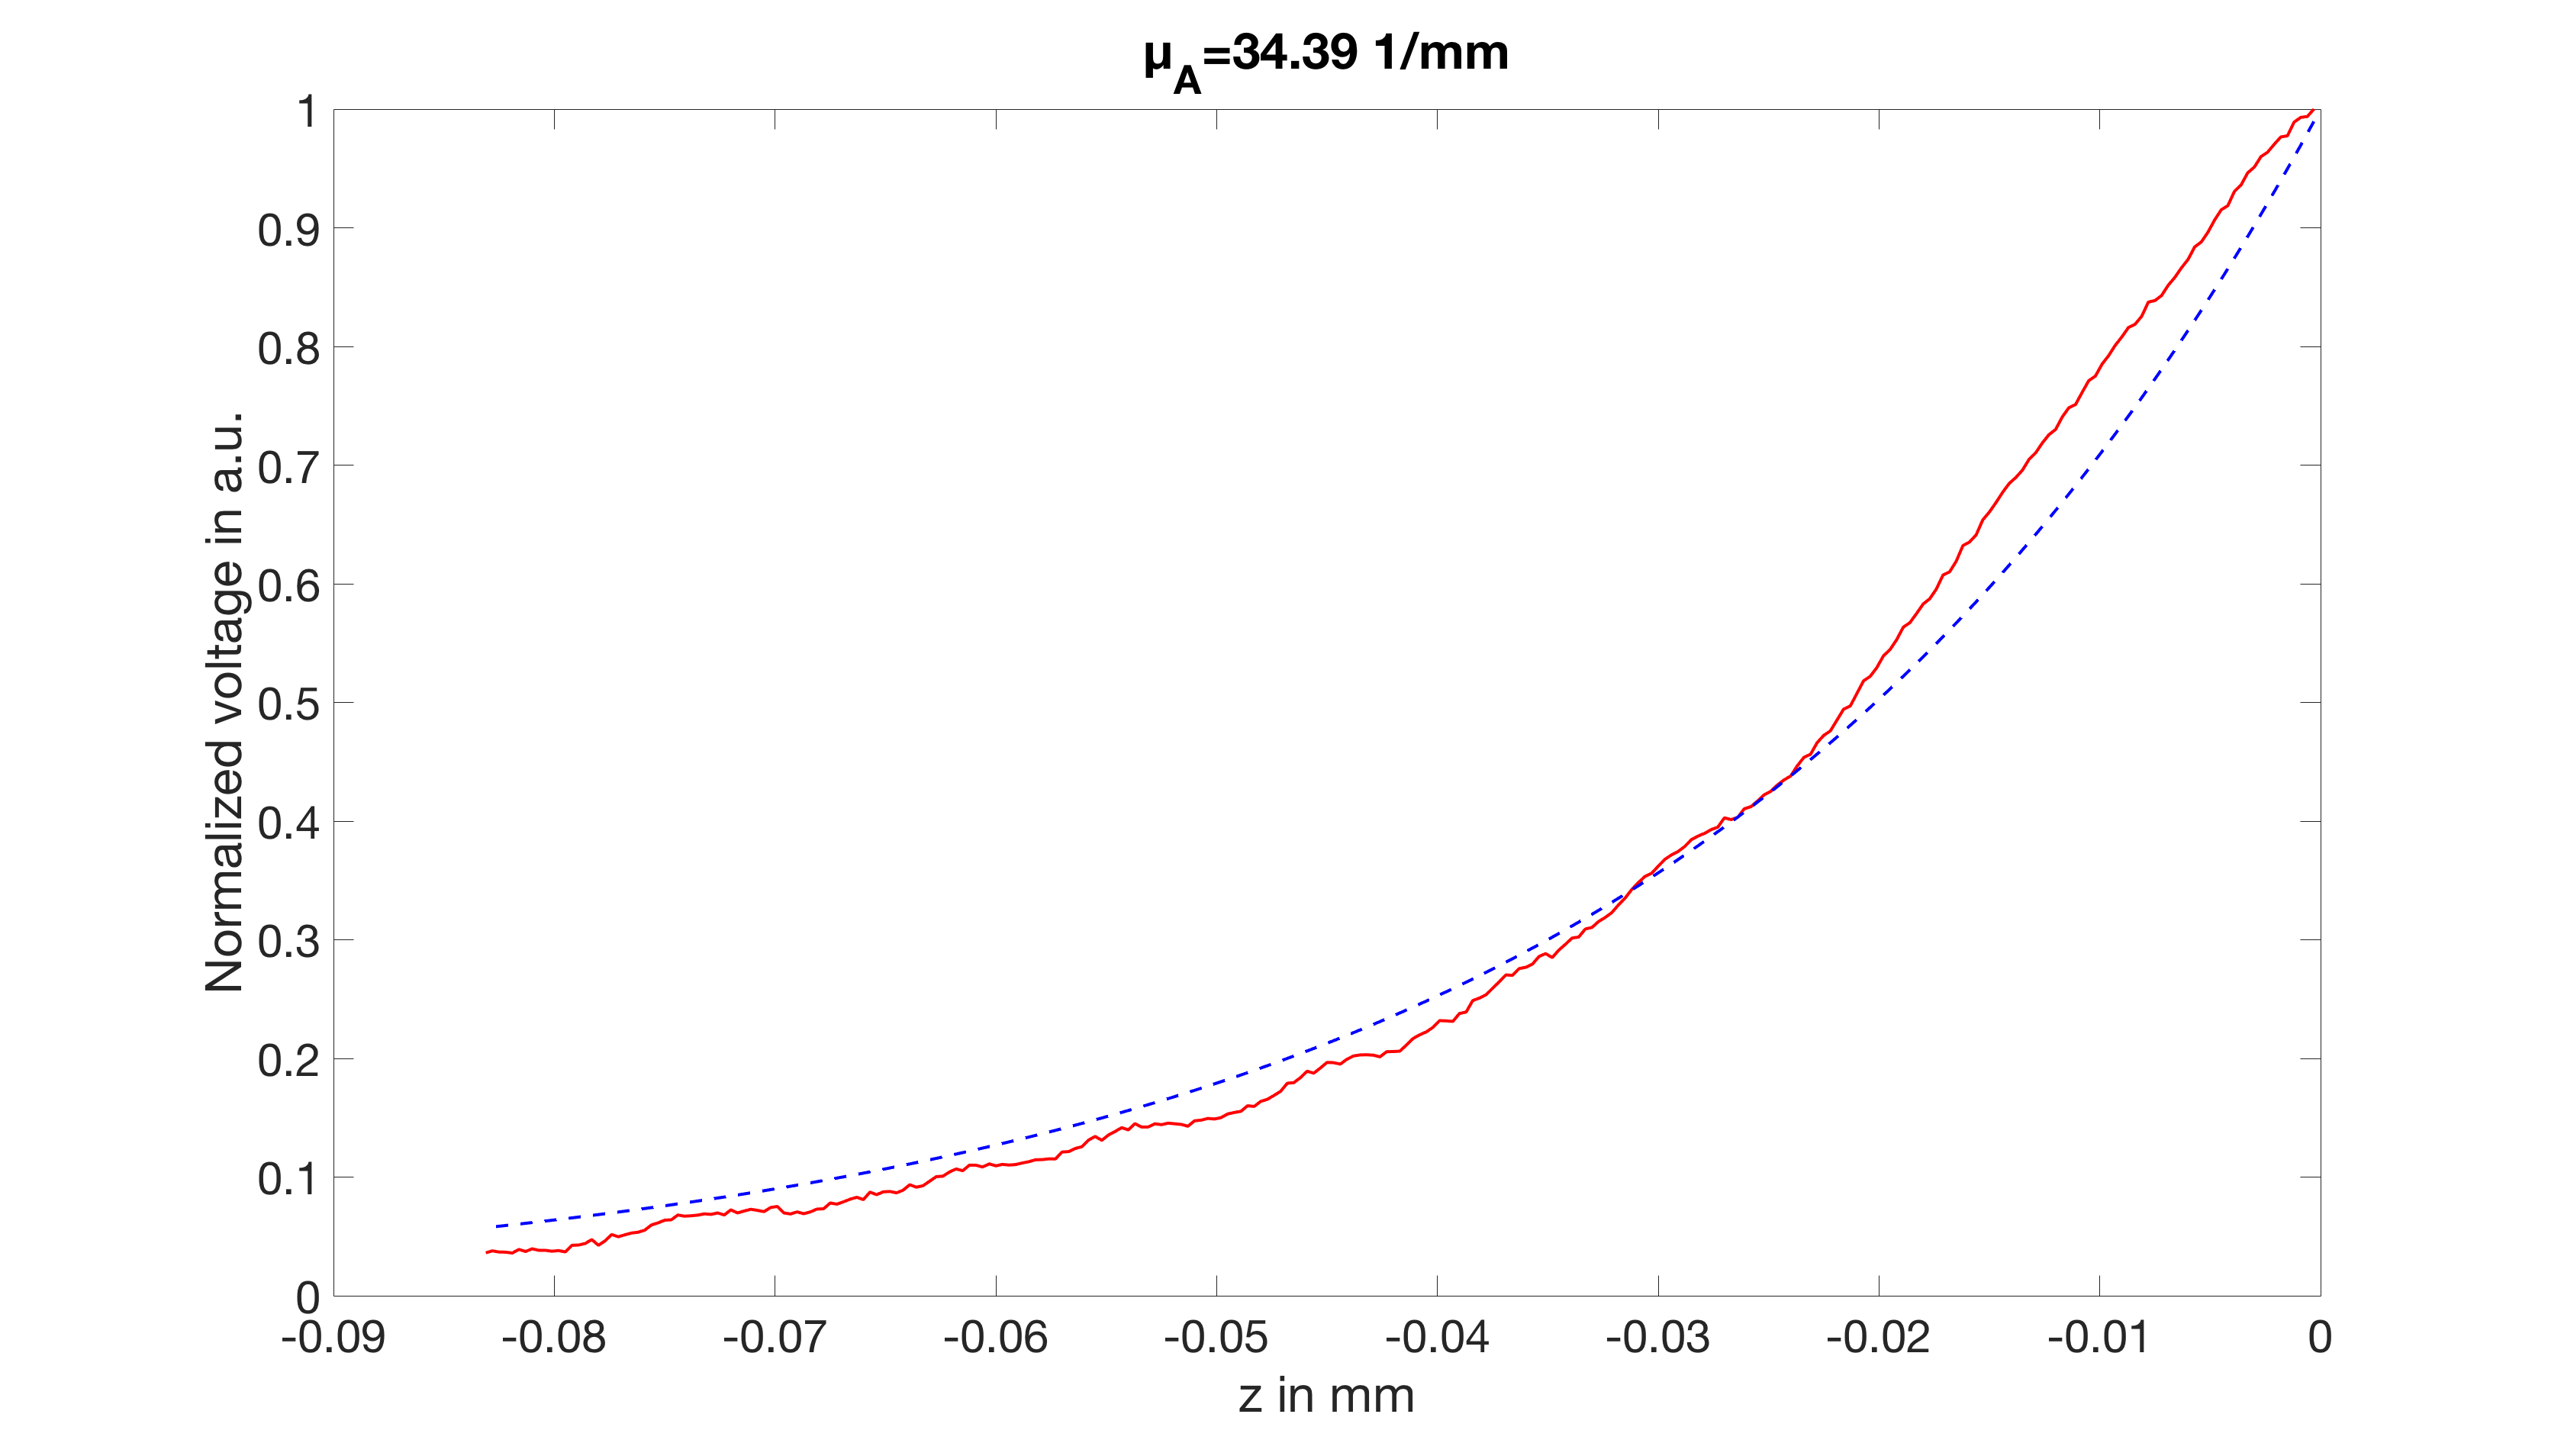
\includegraphics[width = \textwidth, height=0.25\textheight]{03_GR-PAM_theory/images/mu_aFit.png}
	\end{minipage}	
	\caption{In a) a typical PA signal is shown, there the rising part is taken to fit in an exponential function shown in b). The x-axis in b) is converted from a time scale into a depth scale, there zero marks the maximum penetration depth taken. In b) the red line marks the measured data and the dashed blue line is the fit function.}
	\label{fig:mu_aSigFit}
\end{figure}

In figure \ref{fig:mu_aSigFit} the procedure to determine $\mu_a$ is shown. At first a laser pulse were shot onto the liquid and the generated PA signal were recorded. Afterwards the data were loaded into a Matlab program to select the rising edge of the PA signal. A fit function then determines the most suitable $\mu_a$, which is displayed in a plot. 

\subsection{Resolution considerations}
\label{sec:resConGR}

In order to determine the possible theoretical resolution that can be achieved, a 2D Gaussian distribution, for the fluence in lateral direction, can be supposed. The PA$_1$ that is generated by the first laser pulse can be derived by the spatial integration of p$_1$. 

\begin{equation}
	\mathrm{PA}_1 = k_{loss} \Gamma_0 \eta_{th} Q \iint\mu_a(x,y) \frac{1}{\pi w^2} \exp{\left(-\frac{x^2+y^2}{w^2}\right)} \mathrm{d}x\mathrm{d}y
	\label{eq:PA1}
\end{equation}
\\
There the PA is the measured voltage signal. The transformation of a pressure wave into a voltage signal, the detection sensitivity and the appearing losses are considered by a constant $k_{loss}$. For the assumption, that the integration can be performed independently from the z-direction, can be followed, that there are only contributions to k. Further $Q$ is the pulse energy and $w_0$ is the waist of the Gaussian beam shown in Figure \ref{fig:focusWaist} \cite{Bessel:GRPAM, Wang:GRPAM}. 

\begin{figure}[H]
	\centering
	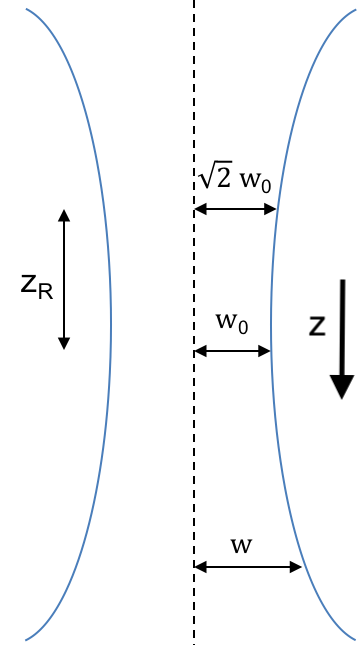
\includegraphics[width = 0.25\textwidth, height=0.3\textheight]{03_GR-PAM_theory/images/focusWaist.png}
	\caption{Optical focus waist, where $w_0$ is the smallest waist radius, $z_R$ the Rayleigh length (distance from $w_0$ there the waist radius is $\sqrt{2}$ $w_0$) and $w$ the distance from the optical axis.}
	\label{fig:focusWaist}
\end{figure}

Analogue to PA$_1$, PA$_2$ is determined by

\begin{multline}
	\mathrm{PA}_2 = \underbrace{k_{loss} \Gamma_0 \eta_{th} Q \iint \mu_a(x,y) \frac{1}{\pi w^2} \exp{\left(-\frac{x^2+y^2}{w^2}\right)} \mathrm{d}x \mathrm{d}y}_{\mathrm{I}} \; + \\ \underbrace{k_{loss} G \eta_{th}^2 Q^2 \iint \mu_a(x,y)^2 \frac{1}{\pi^2 w^4} \exp{\left(-\frac{x^2+y^2}{\frac{1}{2}w^2}\right)} \mathrm{d}x\mathrm{d}y}_{\mathrm{II}}
	\label{eq:PA2}
\end{multline}
\\
Equation \ref{eq:PA2} consists of two parts. Part $I$ is the same as PA$_1$ (\ref{eq:PA1}). But part $II$ is induced by the Grueneisen effect, resulting of the first laser pulse preheating and the excitation of the second laser pulse. The assumption that F$_1$~= ~F$_2$ is still valid. If the generated PA$_1$ is subtracted from PA$_2$, $\Delta \mathrm{PA}$ is given by

\begin{equation}
\begin{split}
	\Delta \mathrm{PA} &= \mathrm{PA}_2 - \mathrm{PA}_1\\
	&= k_{loss} G \eta_{th}^2 Q^2 \iint \mu_a^2(x,y) \frac{1}{\pi^2w^4} \exp{\left(-\frac{x^2+y^2}{w^2/2}\right)} \mathrm{d}x\mathrm{d}y
	\end{split}
\end{equation}
\\
In order to determine the lateral resolution of GR-PAM a point target can be scanned in the x - y plane. Consequently the point spread function is given by 

\begin{equation}
\Delta \mathrm{PA} (x,y) = k_{loss} G \eta_{th}^2 Q^2 \mu_a^2 \frac{1}{\pi^2w^4} \exp{\left(-\frac{x^2+y^2}{w^2/2}\right)} 
\end{equation}
\\
which correspond to a 2D Gaussian distribution with a waist $\sigma$ of $w/\sqrt{2}$. In comparison, OR-PAM gives the following distribution. 

\begin{equation}
\mathrm{PA_{OR-PAM}} (x,y) = k_{loss} \Gamma_0 \eta_{th} Q \mu_a \frac{1}{\pi w^2} \exp{\left(-\frac{x^2+y^2}{w^2}\right)} 
\end{equation}
\\
This follows a $\sigma$ of $w$ and therefore a higher lateral resolution of GR-PAM compared to OR-PAM by the factor $\sqrt{2}$ \cite{PhysRevLett.113.174301}.\\
The axial resolution of GR-PAM can be determined by analyzing the Gaussian beam profile depending on the z-direction, shown in figure \ref{fig:focusWaist}.
There the waist width $w$ is defined by

\begin{equation}
w(z)^2 =  w_0^2 \left(1 + \frac{z^2}{z_R^2}\right)
\end{equation}
\\
The GR-PAM signal for a planar target with uniformly distributed $\mu_a$ is 

\begin{equation}
\Delta \mathrm{PA} = k_{loss} G \eta_{th}^2 Q^2 \mu_a^2 \frac{1}{2 \pi^2w^2} 
\end{equation}
\\
There the OR-PAM signal for the same target is

\begin{equation}
\mathrm{PA_{OR-PAM}} = k_{loss} \Gamma_0 \eta_{th} Q \mu_a 
\label{eq:PA_OR_PAM}
\end{equation}
\\
This follows for $z = \pm z_R$, that the GR-PAM amplitude reduces by half, when the laser beam is focused onto the absorbing plane. Therefore the axial FWHM is $2\cdot z_R$, following optical axial sectioning capabilities for GR-PAM. It is evident that OR-PAM has no optical axial sectioning for planar targets as described by formula \ref{eq:PA_OR_PAM}. Due to no dependence on the focal distance \cite{PhysRevLett.113.174301}.\\
In table \ref{tab:resCompare} the comparison of the possible resolution power for OR-PAM and GR-PAM is collected.

\begin{table}[H]
	\centering
	\caption{Comparison of the theoretical possible resolutions that can be achieved with OR-PAM and GR-PAM \cite{Wang:GRPAM}.}
	\begin{tabular}{| m{1.7cm} | c | c |}
		\hline
		&OR-PAM&GR-PAM \\ \hline
		\centering Axial \newline resolution&no optical resolution&$2\cdot z_R$ \\ \hline
		\centering Lateral \newline resolution&$2 \cdot w_0$&$\sqrt{2} \cdot w_0$\\	\hline
	\end{tabular}	 
	\label{tab:resCompare}
\end{table}




\section{Experimental results of photoacoustic microscopy}
The measurements performed in this section were done with the setup described in section \ref{sec:ORPAMsetup}. As the focus has been on investigating biological tissue with the help of phantom samples, water, ricinus oil (to simulate fat) and a black plastic leaf (to simulate blood vessels) were used.

\subsection{Proof of the Grueneisen effect}
\label{sec:GRpoof}
In order to prove that the photoacoustic amplitude varies with temperature, a small container with either water (colored with OrangeG) or rizinus oil (colored with paprika), was placed on top of a Peltier-element. If a current is applied to this component, one side heats up and its backside cools down. The container were placed onto the hot side and the temperature were tracked by a thermo element. OrangeG is a dye, with a yellow-orange appearance, which has a good solubility in water. Furthermore, its $\mu_a$ is comparable to the $\mu_a$ of blood in the 532~$nm$ range \cite{data:OrangeG}.\\
At first a current were applied to the Peltier-element to meet the start temperature of 30~$^\circ C$. For every measurement the temperature were held 2 minutes at a constant value to guarantee a thermal equilibrium at the desired temperature. After this rest time a burst of ten laser pulses, with a repetition rate of 100~$Hz$, were applied to the sample and the photoacoustic amplitude were detected. Afterwards the temperature gets incremented by 3~$^\circ C$ up to the stop temperature of 60~$^\circ C$. The collected data were visualized in Figure \ref{fig:measuredGRproof}.
 
\begin{figure}[H]
a)
\begin{minipage}{\textwidth}

	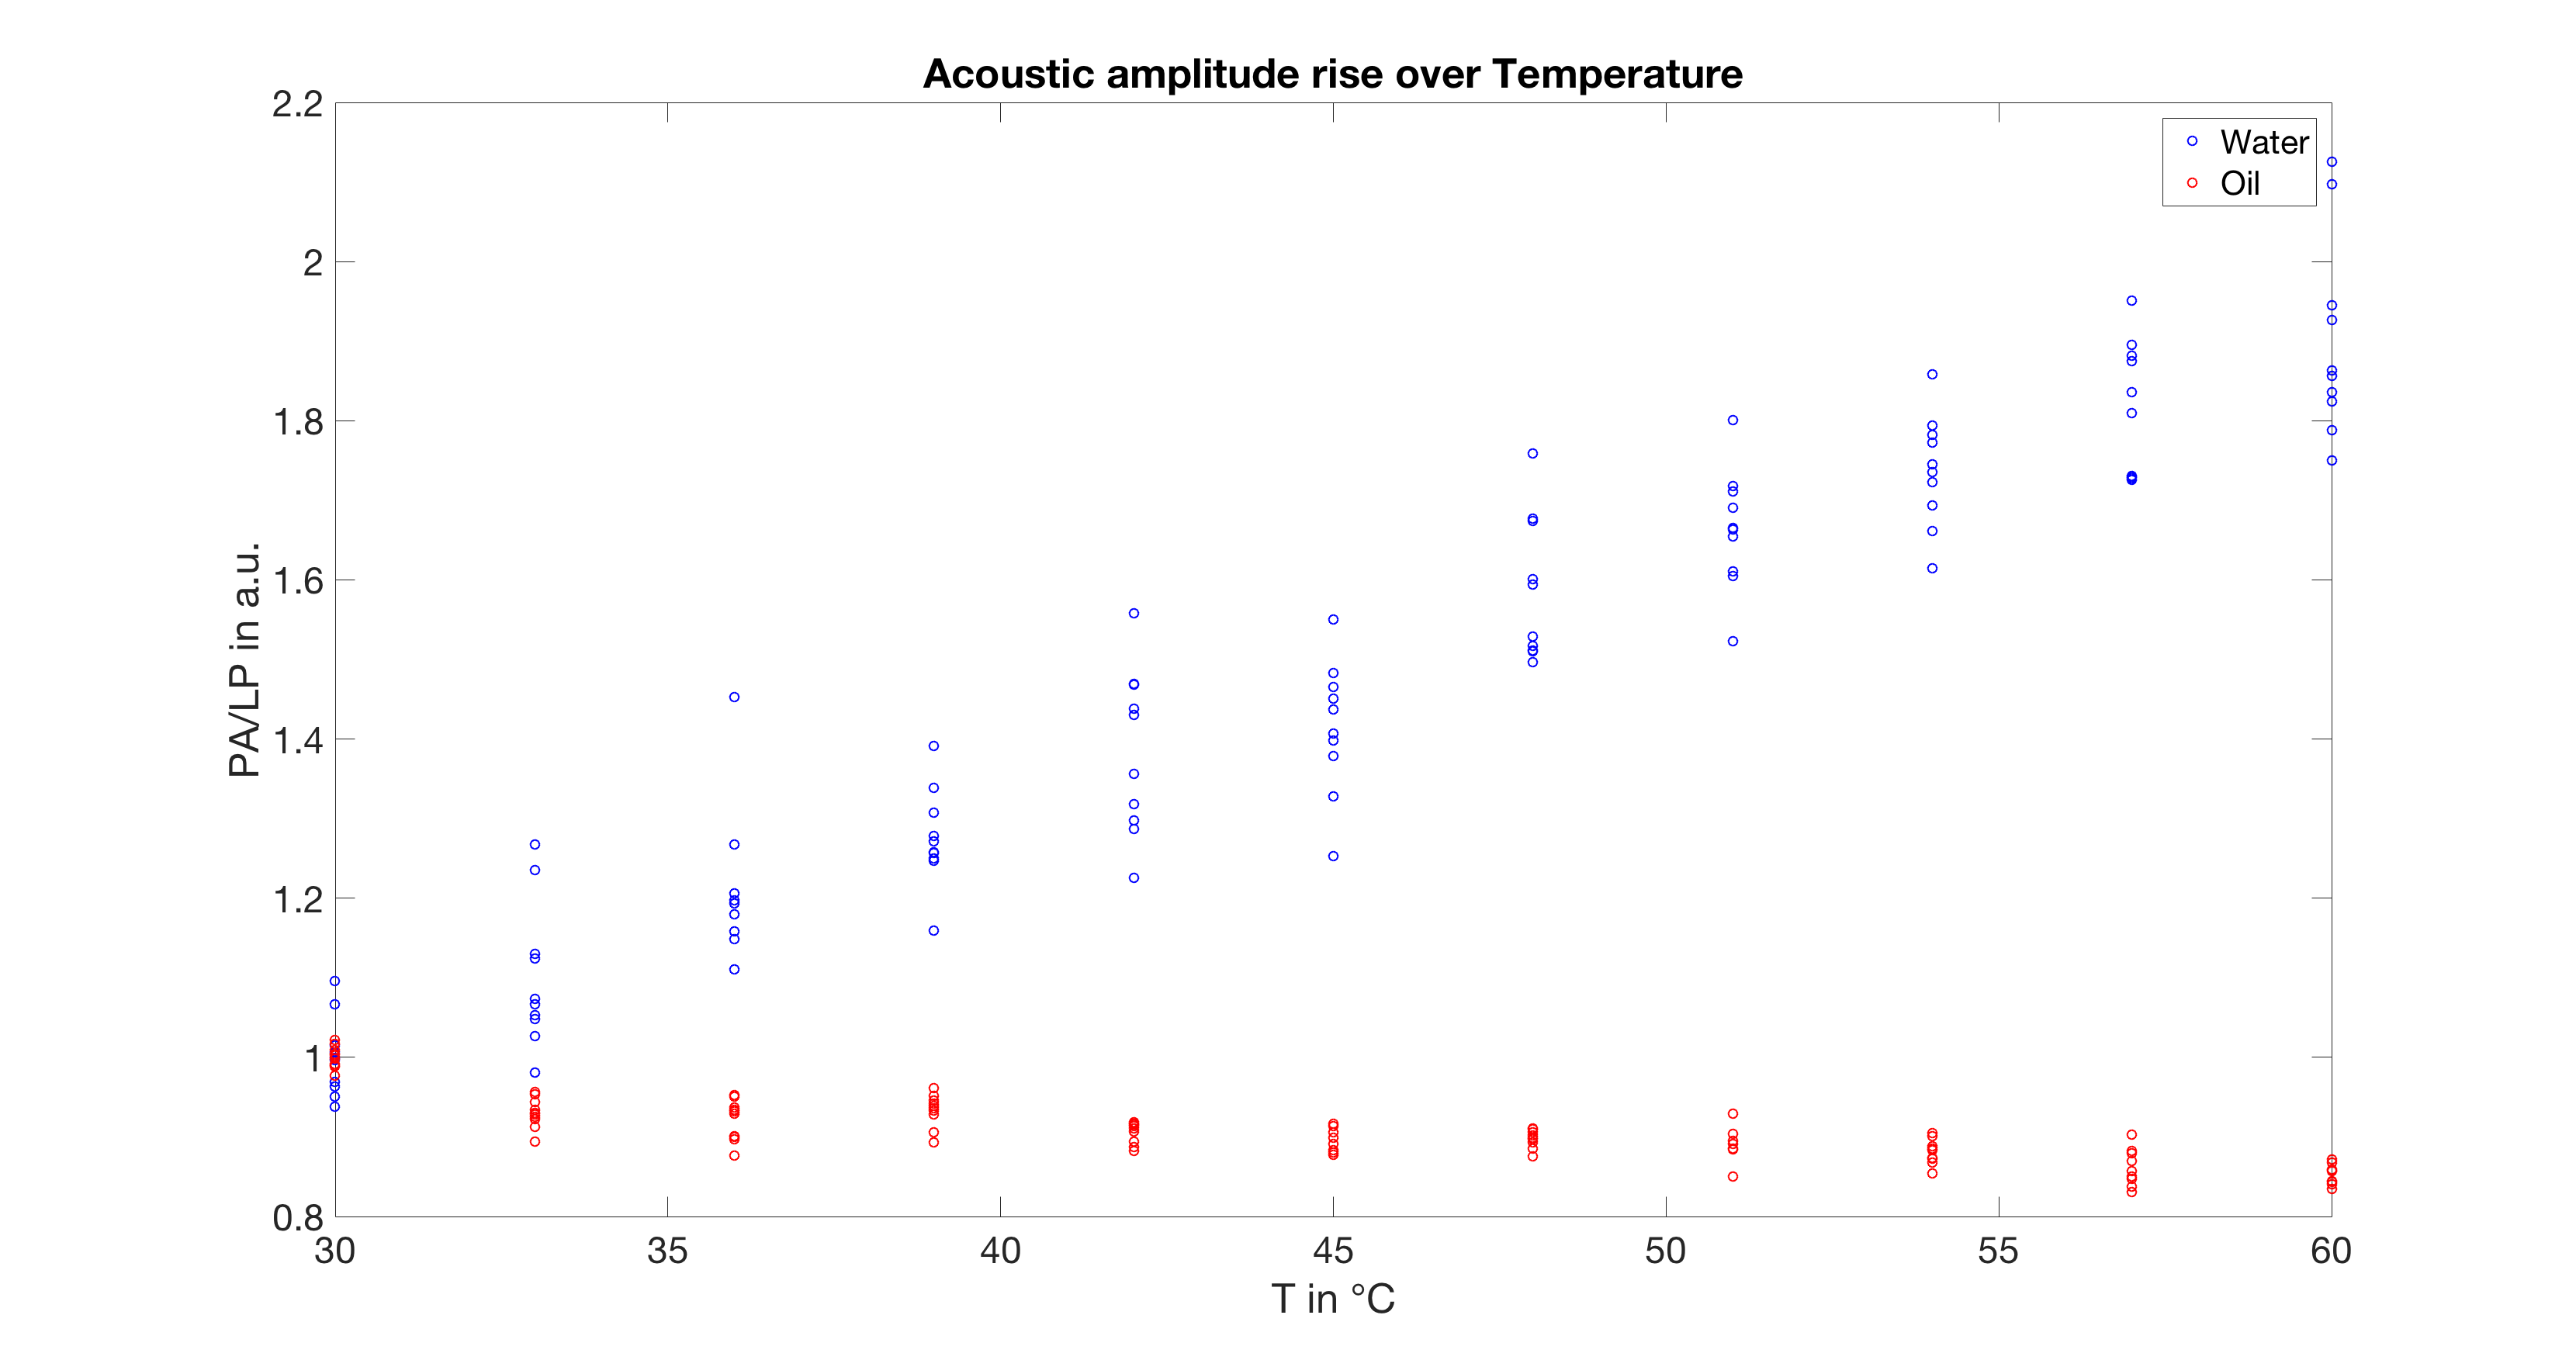
\includegraphics[width = \textwidth, height=0.35\textheight]{04_ex-results_of_PAM/images/GRproof.png}
\end{minipage}
b)
\begin{minipage}{\textwidth}

	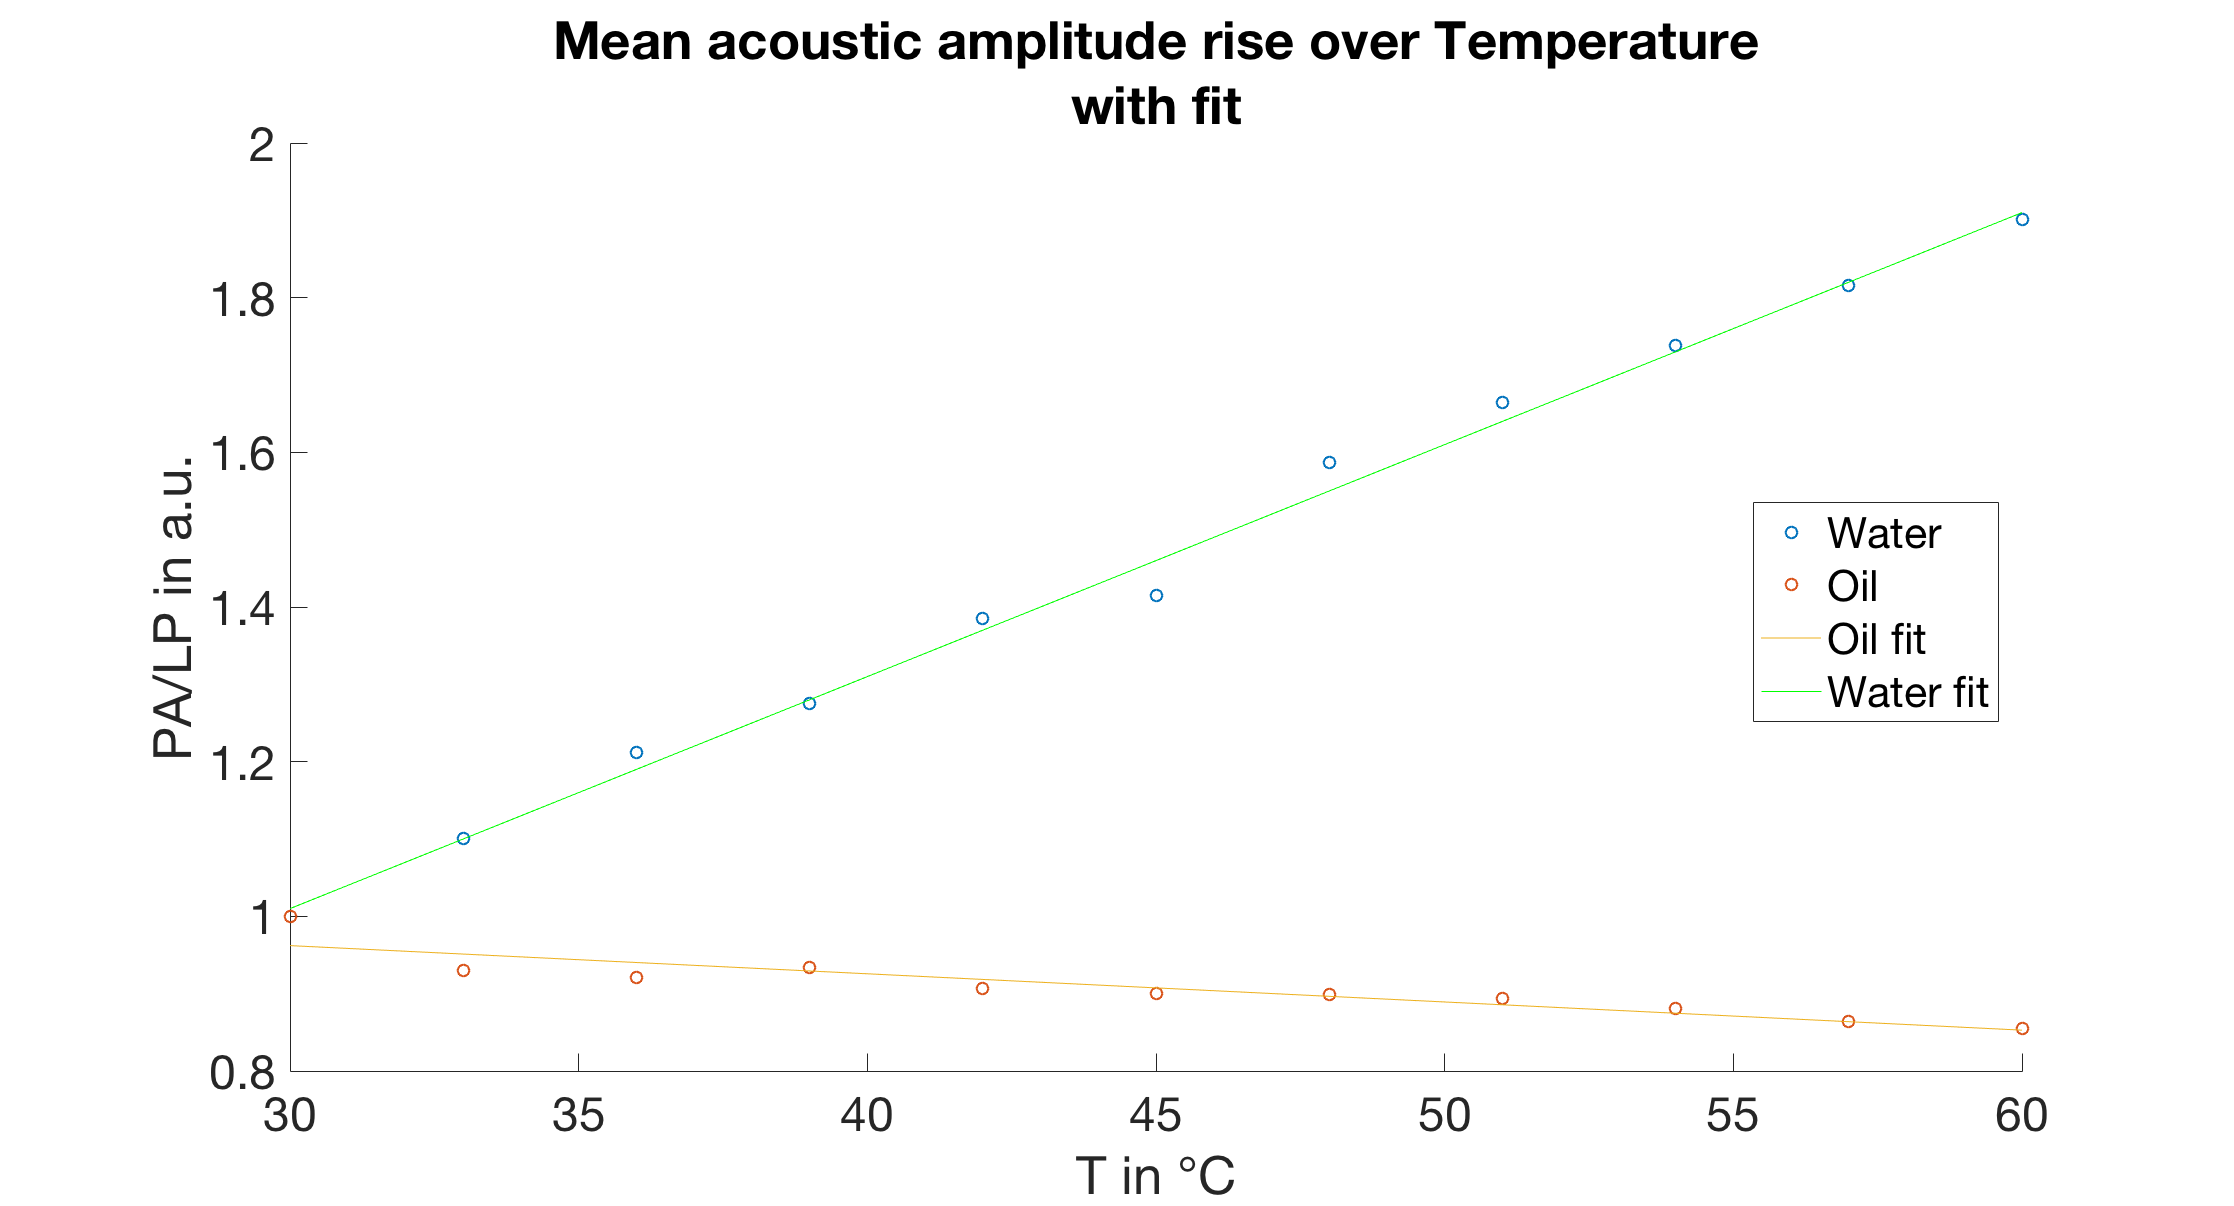
\includegraphics[width = \textwidth, height=0.35\textheight]{04_ex-results_of_PAM/images/meanGRproof.png}
\end{minipage}

\caption{In a) the sampled data for water and oil is displayed and in b) a fit is drawn through the mean values of a). The fit functions are $f_{oil}(T) = -0.0036 \cdot T +1.1$ and $f_{water}(x) = 0.03 \cdot T + 0.11$. The plots in a) and b) are normalized to the mean value at 30~$^\circ C$ and also the photoacoustic amplitudes are normalized to the laser power (LP).}
\label{fig:measuredGRproof}
\end{figure}

In Figure \ref{fig:measuredGRproof} b), it can be seen, that the photoacoustic amplitude for water nearly doubles if the temperature is increased from 30~$^\circ C$ to  60~$^\circ C$, while the effect is weaker for oil and is going in the opposite direction.\\
The photoacoustic amplitudes are normalized to the laser power and the dye is uniformly distributed, so that a constant $\mu_a$ can be assumed. According to equation \ref{eq:p_0}, it can be concluded that the increased (water) or decreased (oil) amplitude is a consequence of a changed $\Gamma$. This leads to a applicable contrast mechanism, here for water and oil, as shown in section \ref{sec:GReffect}.\\
Additional there is to mention that for biological issues, temperatures close to or below 0~$^\circ C$ make no sense to investigate, because of the freezing point of water. But it is crucial not to exceed the boiling point of 100~$^\circ C$. Therefore it is important to keep the laser power for GR-PAM in certain limits to avoid cavitation or ablation, but it has to be strong enough to apply a certain temperature rise. 

\subsection{Experimental results of GR-PAM}

The verified Grueneisen effect were applied to microscopy. Therefore, the used system is described and GR-PAM is compared to OR-PAM. Additionally properties of the used specimen, OrangeG dyed water and paprika powder stained rizinus oil, are determined.

\subsubsection{GR-PAM laser setup}

In order to employ two laser pulses for GR-PAM to the system several setups are possible. By virtue of needing a time delay between the pulses in the $\mu s$ range the laser systems available (All of them have a 10kHz repetition rate) are to slow to use a single one. Therefore a two laser system were built.\\
As basis the OR-PAM setup (introduced in section \ref{sec:ORPAMsetup}) were used and reamed with the part inside the dashed box in figure \ref{fig:GRPAMsetup}. In a first setup version the chosen Laser B was a cw-laser from Spectra-Physics (Excelsior-532-100, $\lambda$ = 532~$nm$) and B* were a liquid crystal retarder (Thorlabs LCC 1233-A). This element changes the polarization of incoming light due to the applied voltage. The control unit of the LCC allows to save two voltage values that can be toggled due to an external trigger. If one value is chosen in a way, that there is the maximum laser power after the beam splitter (BS) and the other one with non, it can be used as a switch for the cw-laser beam. 

\begin{figure}[H]
	\centering
	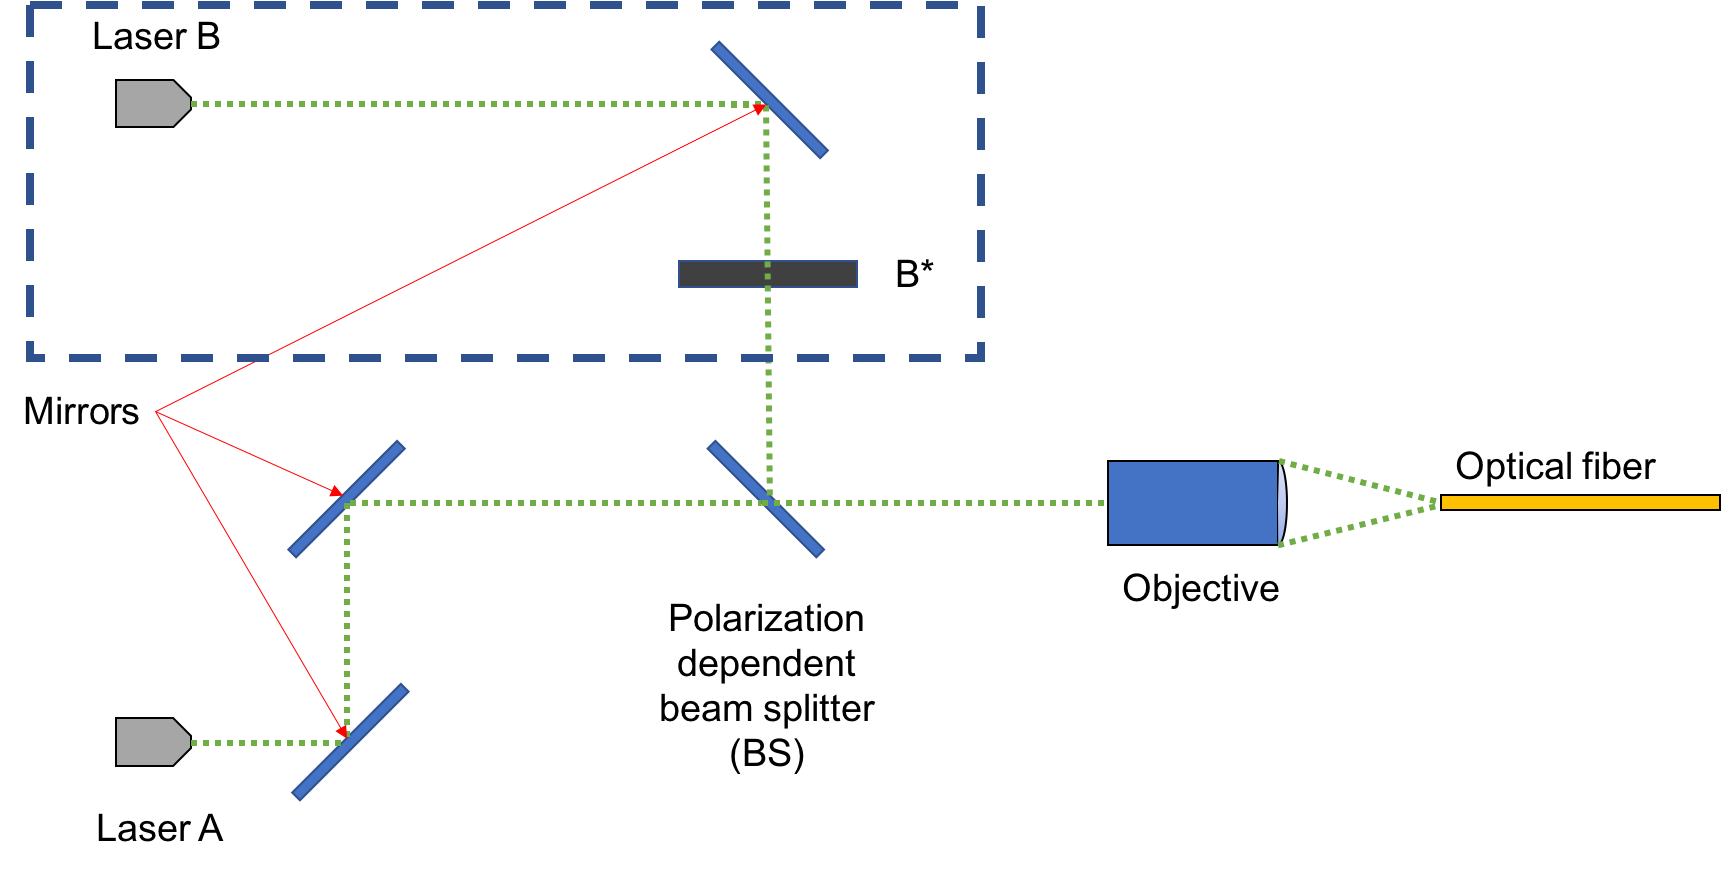
\includegraphics[ height=0.35\textheight]{04_ex-results_of_PAM/images/GR_PAMsetup.png}
	\caption{Illustrated GR-PAM setup. The part inside the dashed box is the part added to the OR-PAM setup to do GR-PAM. Laser A is a LCM-DTL-319QT with $\lambda$ = 527$nm$.}
	\label{fig:GRPAMsetup}
\end{figure}

The disadvantage of this configuration is that the LCC has a rise time $t_r$ of about 500~$\mu s$ and a fall time $t_f$ of 25~$ms$. This leads to a slow scan velocity. \\
In order to increase the scan speed, the dashed part were replaced and only the deflection mirror remains. Laser B were substituted by a pulsed laser (Innolas mosquitoo $\lambda$ = 532~$nm$) and B* with a wave plate that is mounted on a rotary mount. This allows a tuning of the laser power of Laser B that is coupled into the optical fiber. Thus both lasers have a repetition rate of 10~$kHz$, the limiting factor is the maximum possible scan speed the linear stages and scanhead can move. \\
The triggering of the lasers and therefore the delay time between the pulses were generated by the Delay Generator mentioned before.

\subsubsection{Absorption coefficient of OrangeG and colored rizinus oil}
\label{sec:oGrizOilabsoption}
As shown in figure \ref{fig:GRPAMsetup} the two used laser systems, for the GR-PAM measurements, have differing wavelengths. In most cases the absorption difference is negligible, meaning case 1) in section \ref{sec:dualPulseTechnique} is valid. But in some cases option 2) or 3) emerge.\\
However, in Figure \ref{fig:orangeGricinus} the absorption coefficient for OrangeG and, as a reference, the also used paprika powder colored rizinus oil is shown. The OrangeG were dissolved in water with a concentration of 10~$g/l$. The concentration of paprika dye in the oil is unknown. 

\begin{figure}[H]
	\centering
	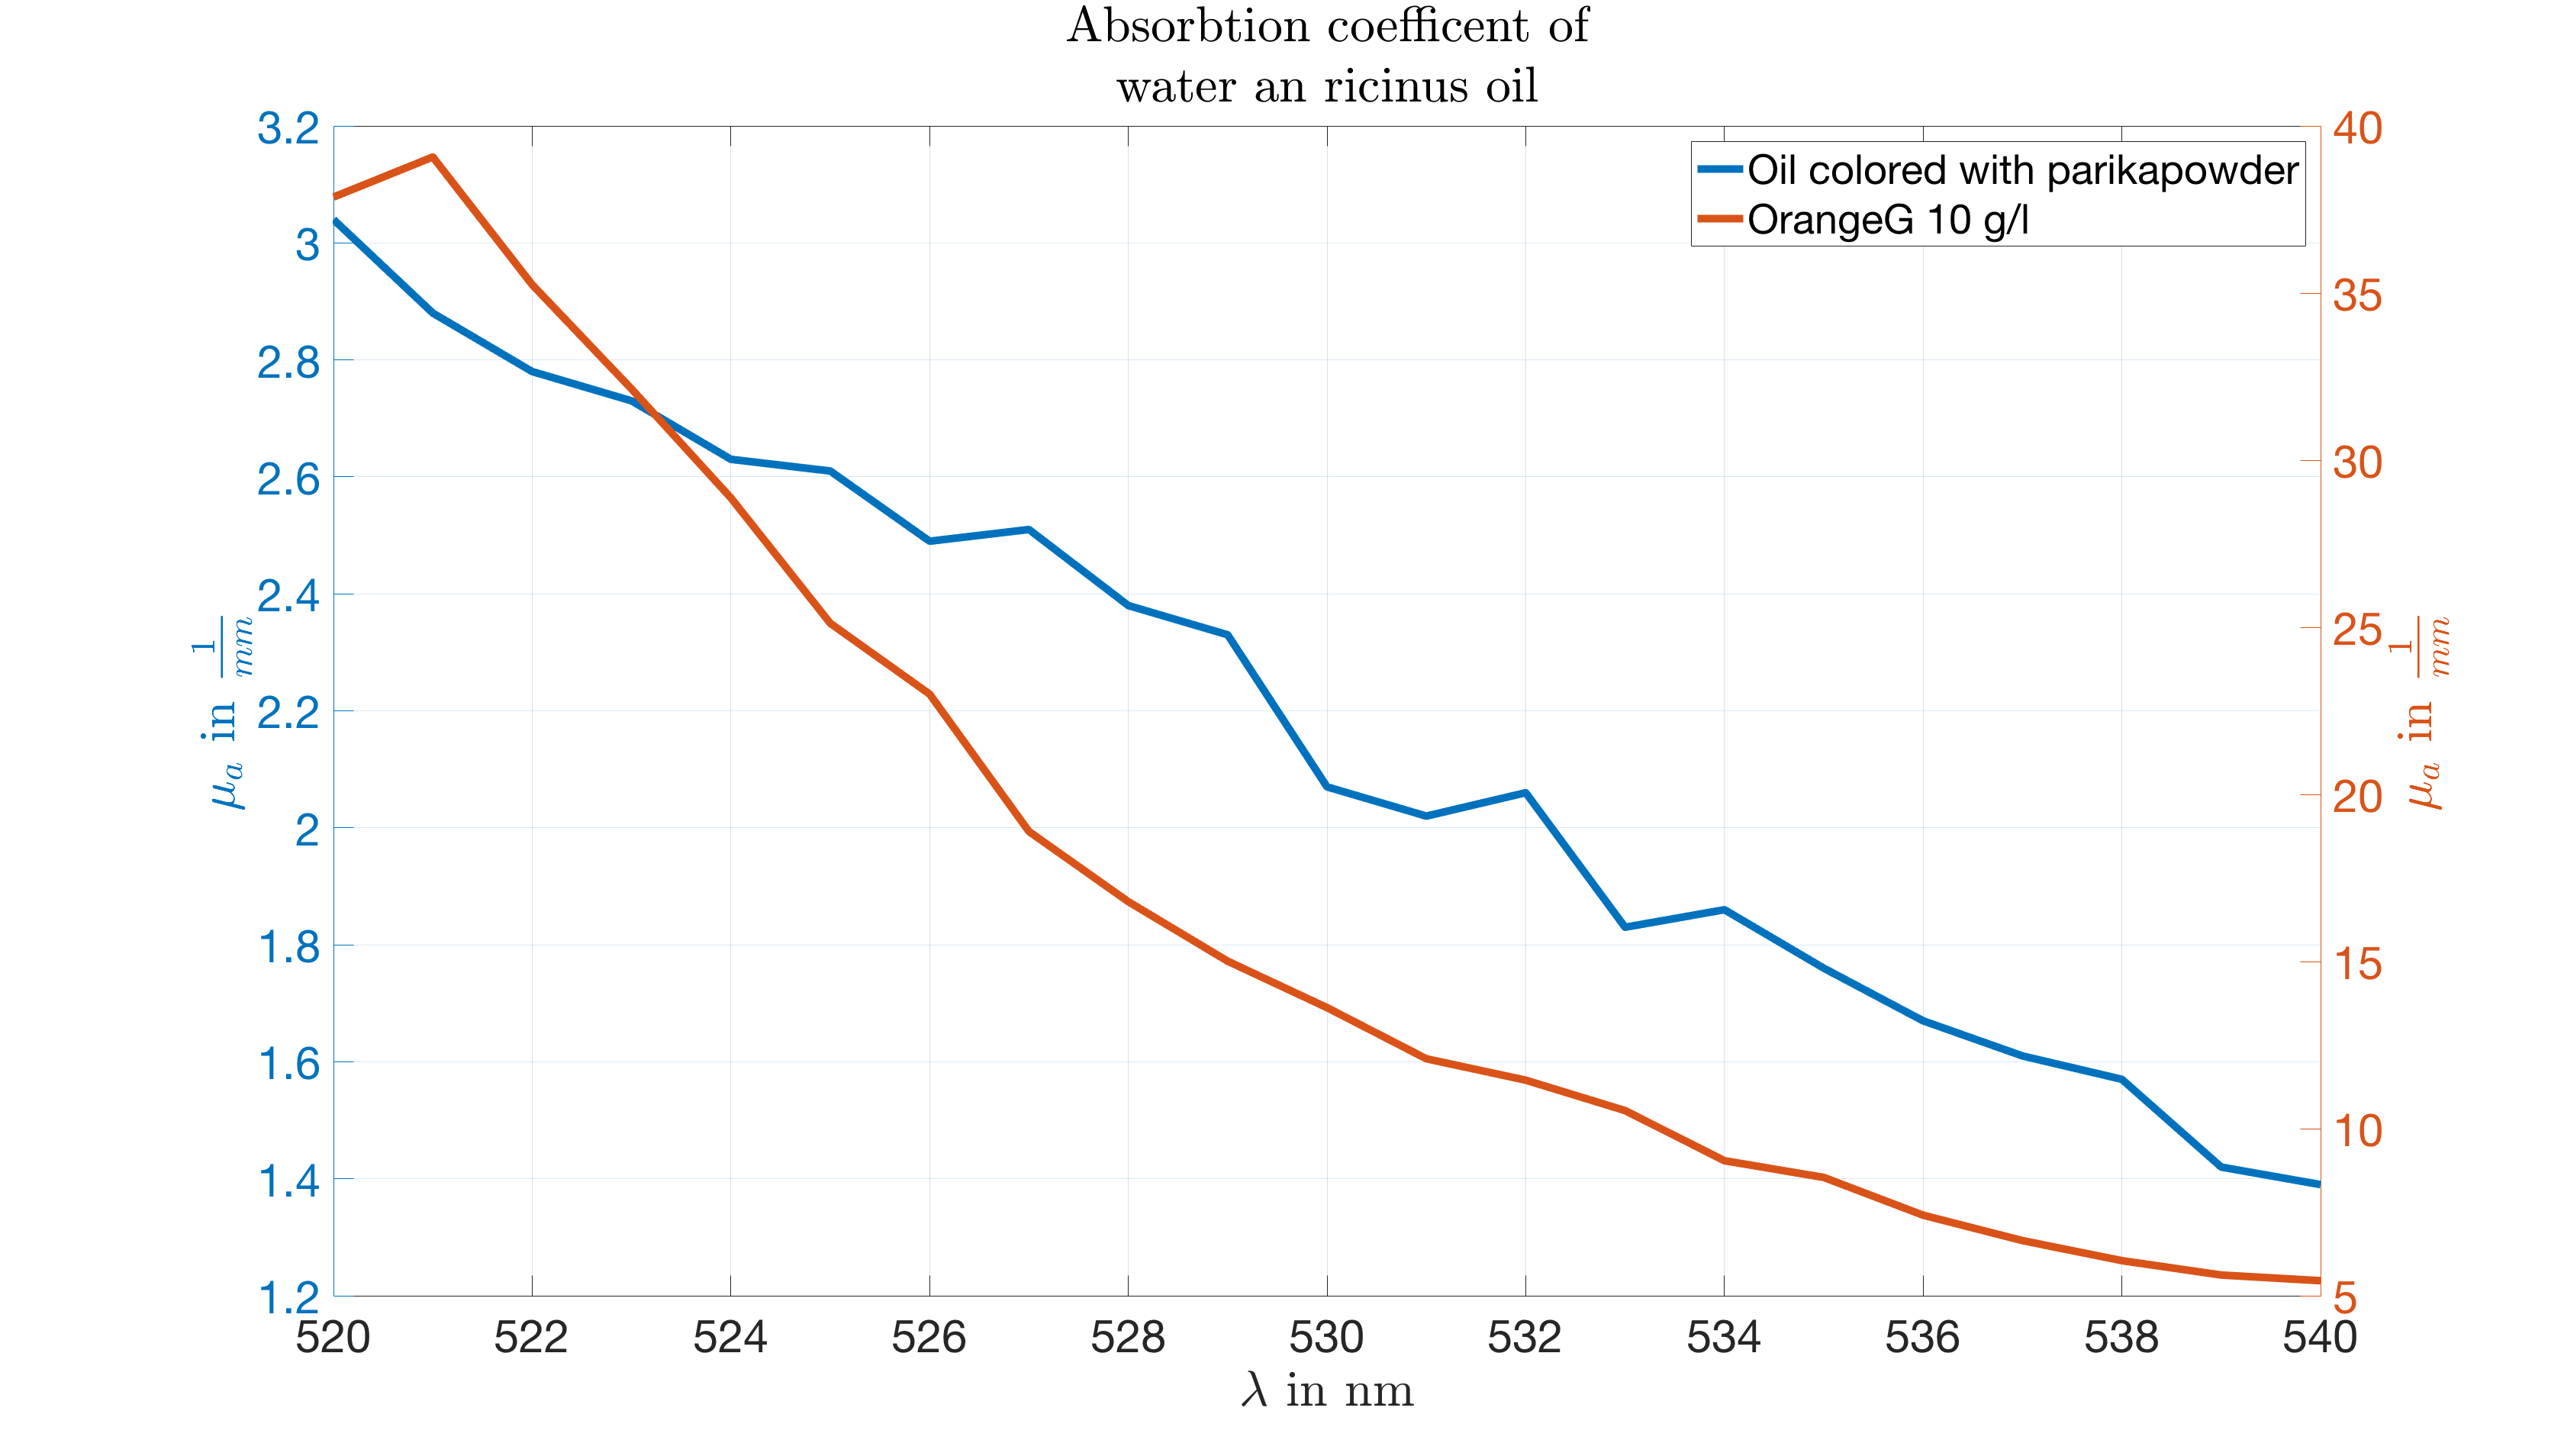
\includegraphics[ height=0.35\textheight]{04_ex-results_of_PAM/images/orangeGricinusMu_a.png}
	\caption{Absorption coefficient of OrangeG dissolved in water and ricinus oil colored with paprika powder, in a wavelength range of 520~$nm$ to 540~$nm$.}
	\label{fig:orangeGricinus}
\end{figure}

It can be seen that there is a difference between the absorption coefficient values for the used wavelengths (527~$nm$ and 532~$nm$). This results for the rizinus oil $\Delta\mu_a$ = 0.45~$\frac{1}{mm}$ and $\Delta\mu_a$  = 7.44~$\frac{1}{mm}$ for OrangeG.\\
Therefore, it is to be considered that the measurements, there OrangeG were used, are done with configuration two. Thus the 532~$nm$ laser were used to operate the heating pulse and the 527~$nm$ laser the detection pulse.

\subsubsection{Comparison between OR-PAM and GR-PAM}
\label{sec:ORGRcomp}

In order to compare OR-PAM with GR-PAM a small container were filled with OrangeG colored water and a droplet of paprika powder colored rizinus oil were deposited. In respect of the results of section \ref{sec:oGrizOilabsoption} the 532$nm$ laser were chosen to apply the heating pulse and the 527$nm$ the detection pulse. Figure \ref{fig:imgGRproof} shows the taken image. 

\begin{figure}[H]
	a)
	\begin{minipage}{\textwidth}
		\centering	
		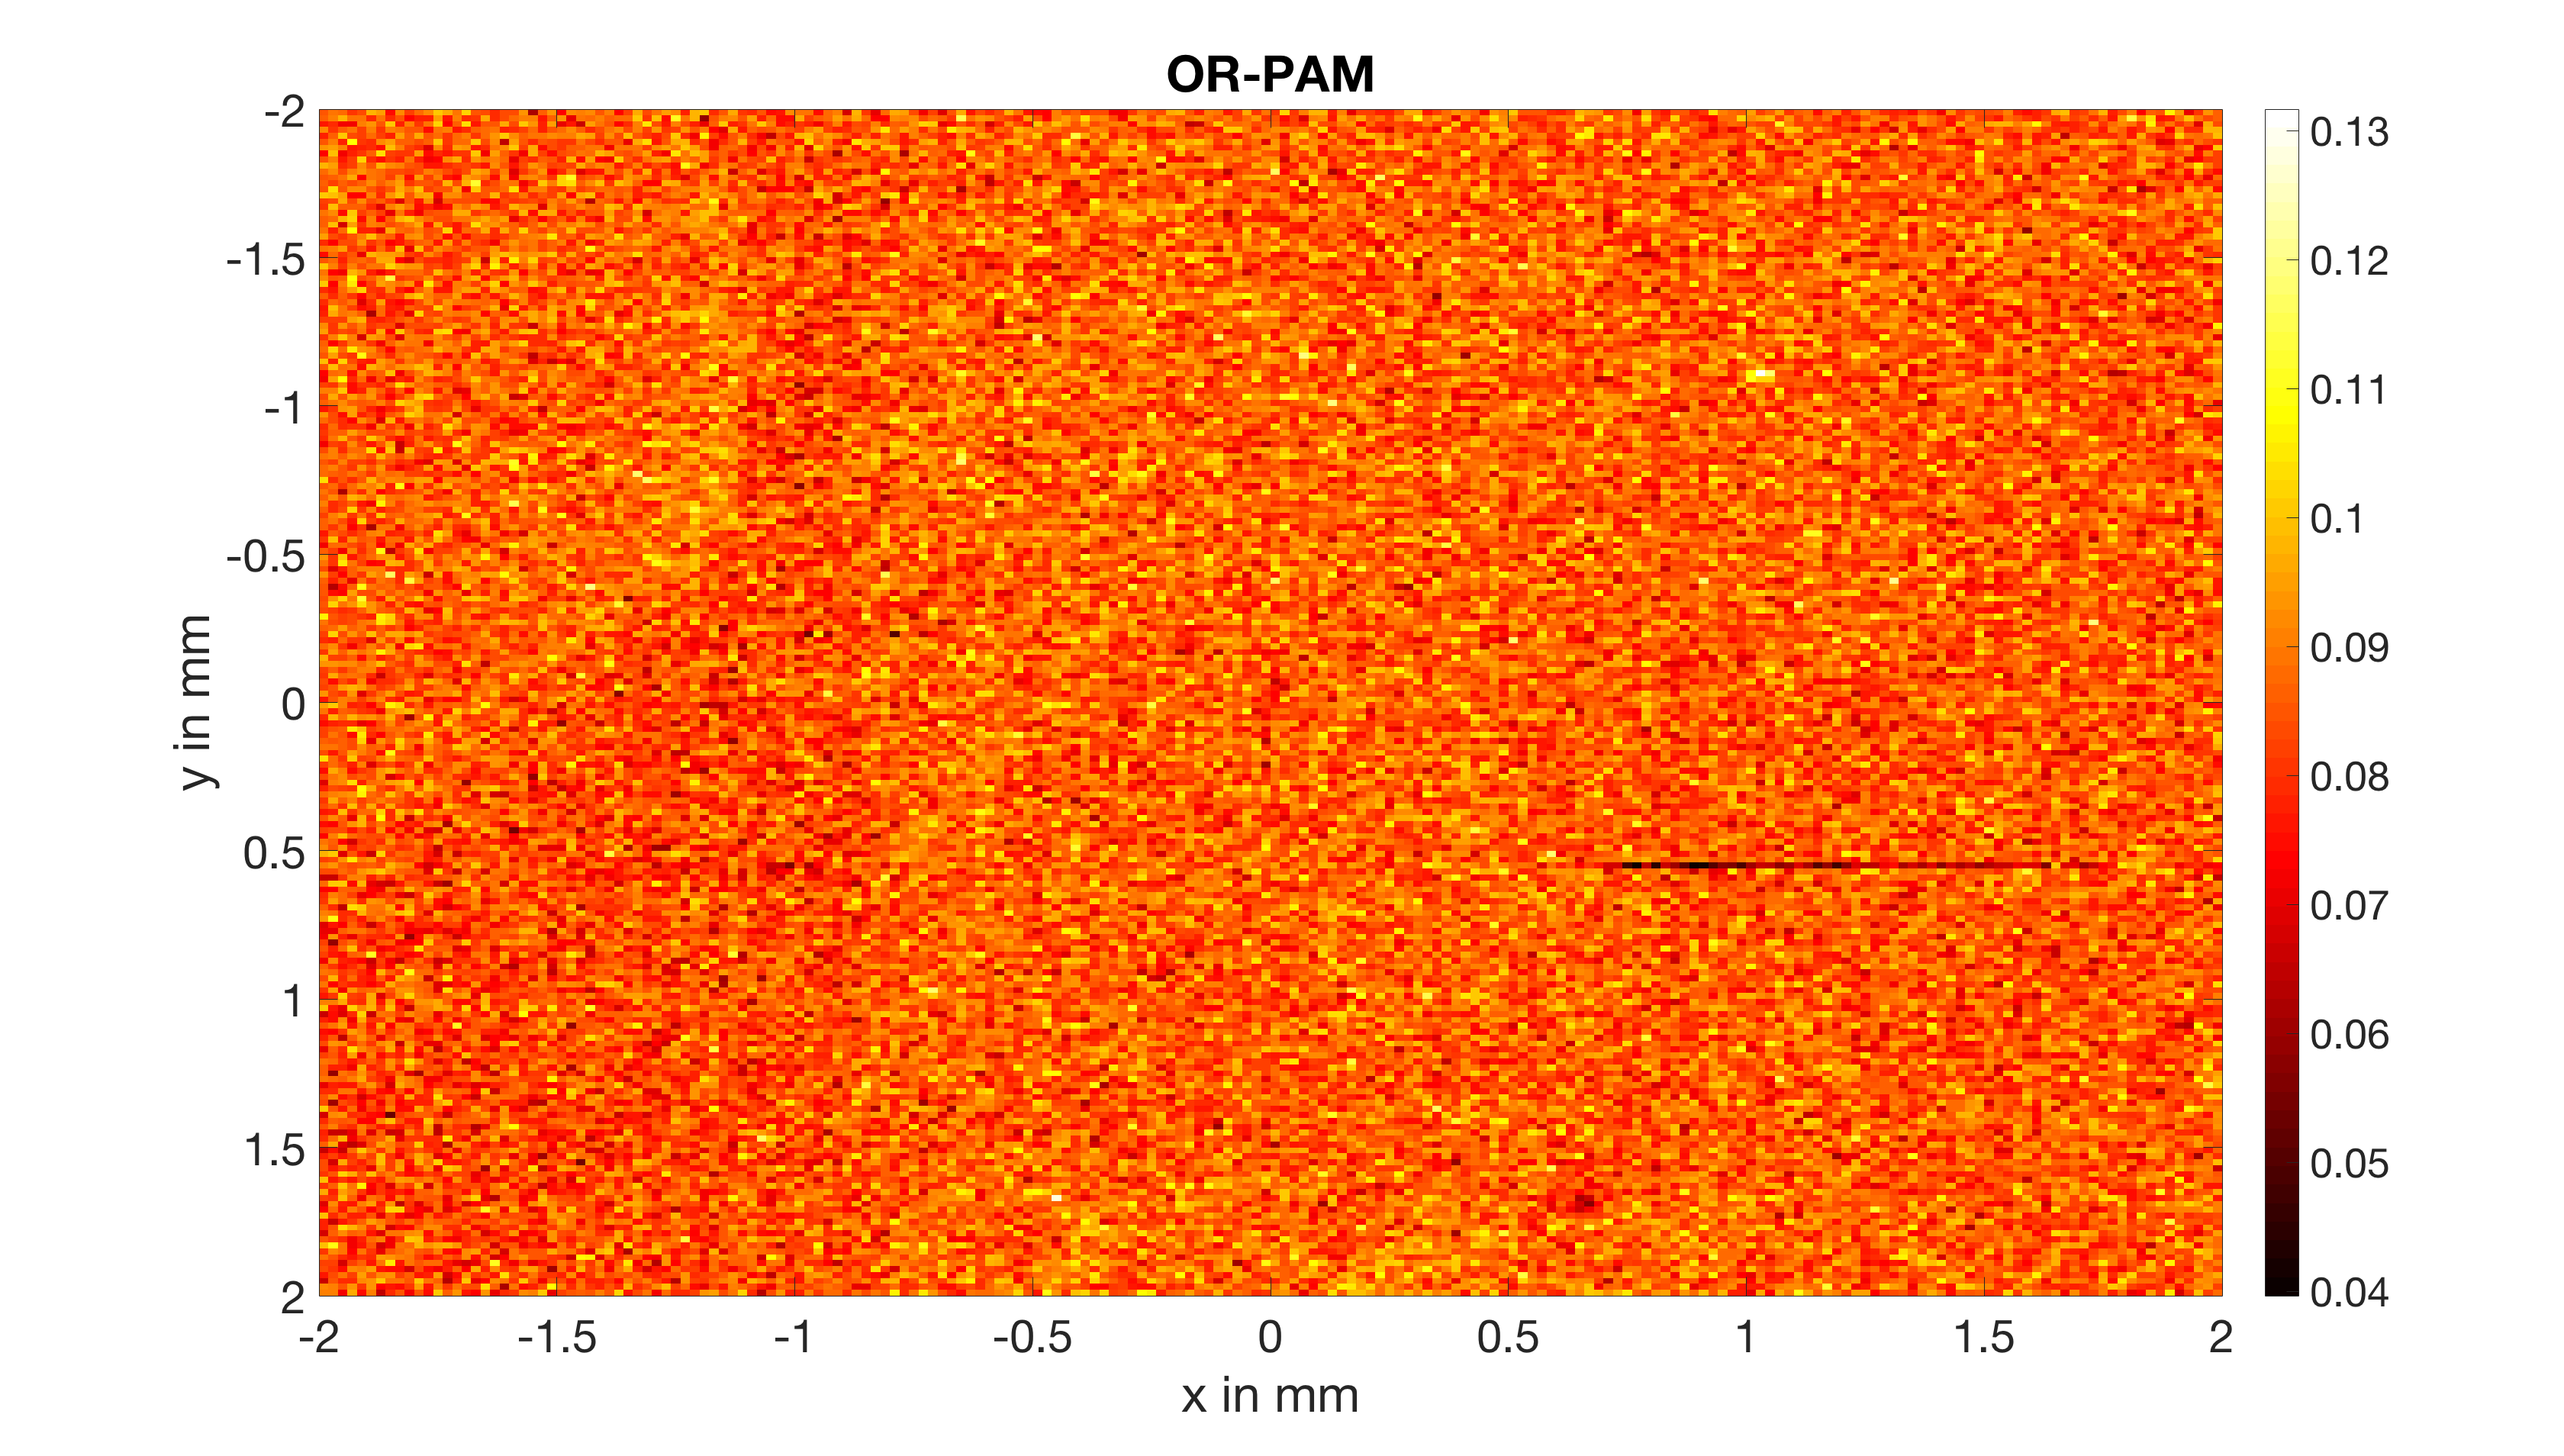
\includegraphics[width = 0.8\textwidth, height=0.38\textheight]{04_ex-results_of_PAM/images/oilDrop_OR.png}
	\end{minipage}	
	b)
	\begin{minipage}{\textwidth}
		\centering	
		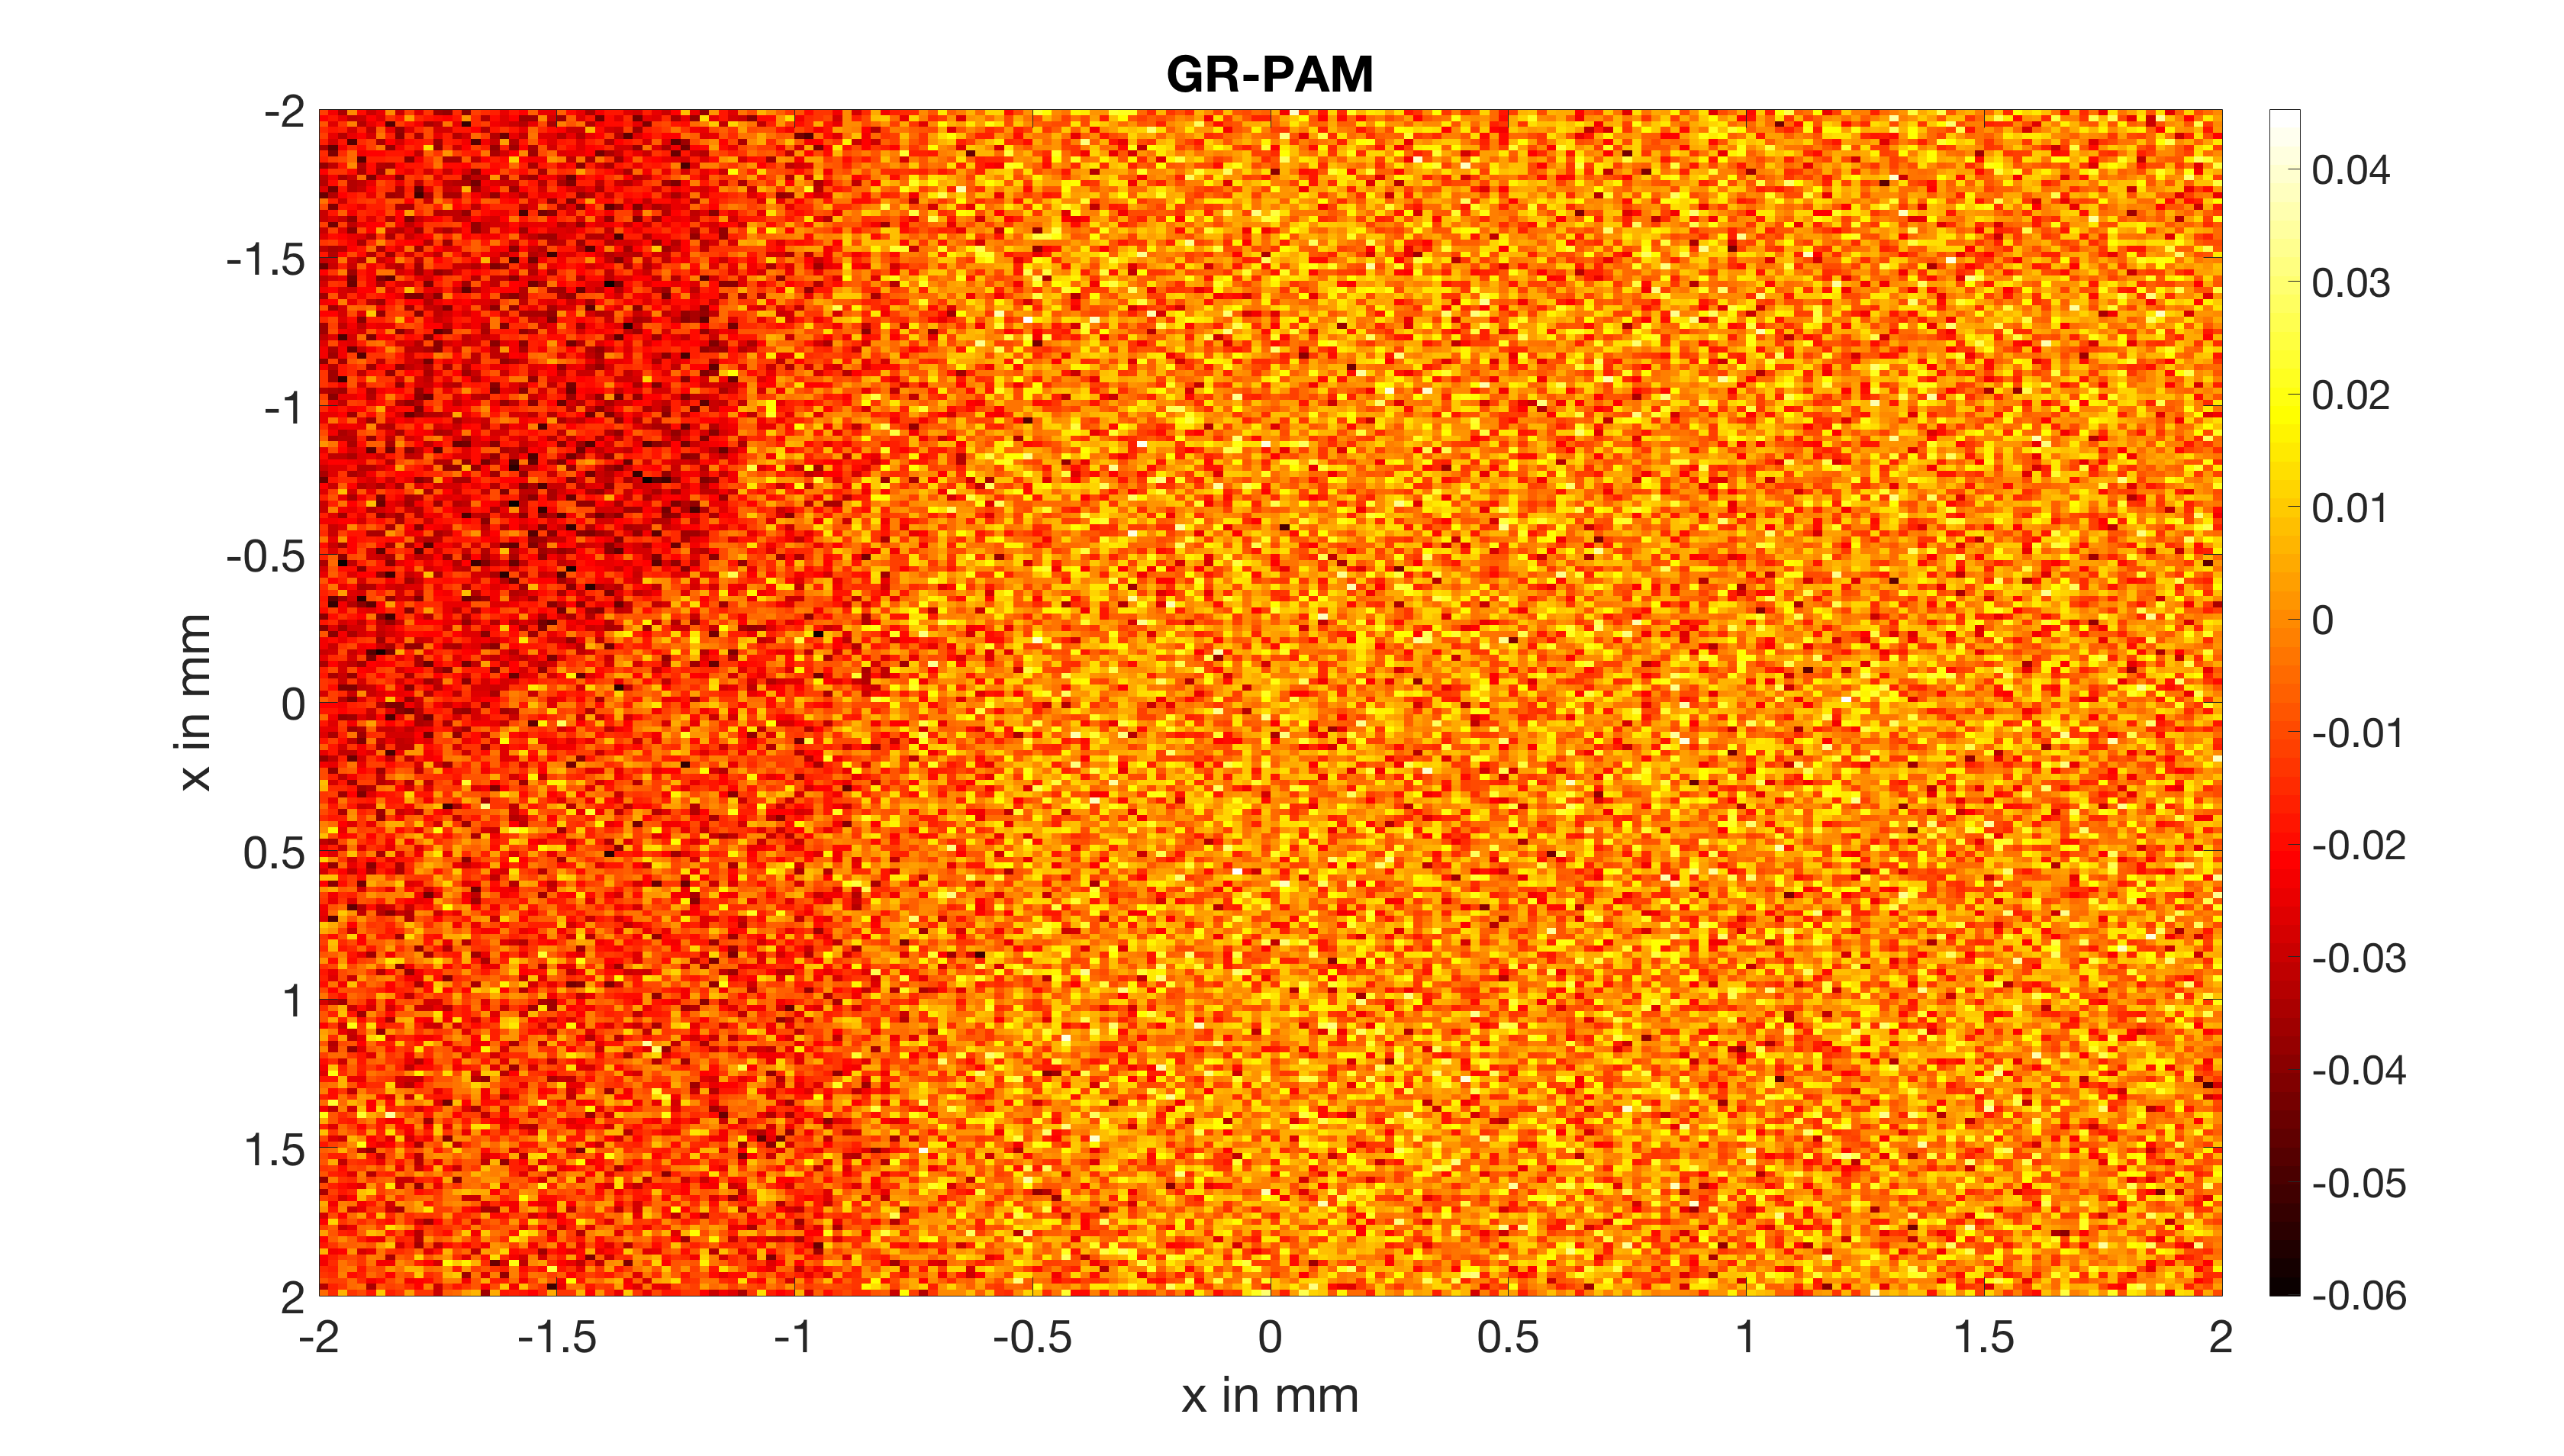
\includegraphics[width = 0.8\textwidth, height=0.38\textheight]{04_ex-results_of_PAM/images/oilDrop_GR.png}
	\end{minipage}
	
	\caption{Image of a rizinus oil droplet in a OrangeG reservoir. The scan area is 4 x 4~$mm$ with 200 points and a step size of 20~$\mu m$ taken in each direction.}
	\label{fig:imgGRproof}
\end{figure}

The oil droplet is placed in the upper left corner of the container. \\
Figure \ref{fig:imgGRproof} a) shows the OR-PAM image, there just the slight differences in the absorption coefficient are visible. The OR-PAM information is taken from the photoacoustic amplitude generated by the first laser pulse. Whereas figure \ref{fig:imgGRproof} b) shows the contrast between the positive Grueneisen effect for the OrangeG colored water and the negative for the rizinus oil.\\
It is important to mention, that the evaluation program takes the maximum amplitude of each data vector, the heating pulse as well as the detection pulse vector. Assuming that the whole two vectors are subtracted from each other, to generate the GR-PAM information, a slight time difference between the peaks results in a wrong representation of the effect.\\
For figure \ref{fig:imgGRblackleaf} a black plastic leaf is imaged.\\

\begin{figure}[H]
	a)
	\begin{minipage}{\textwidth}
		\centering		
		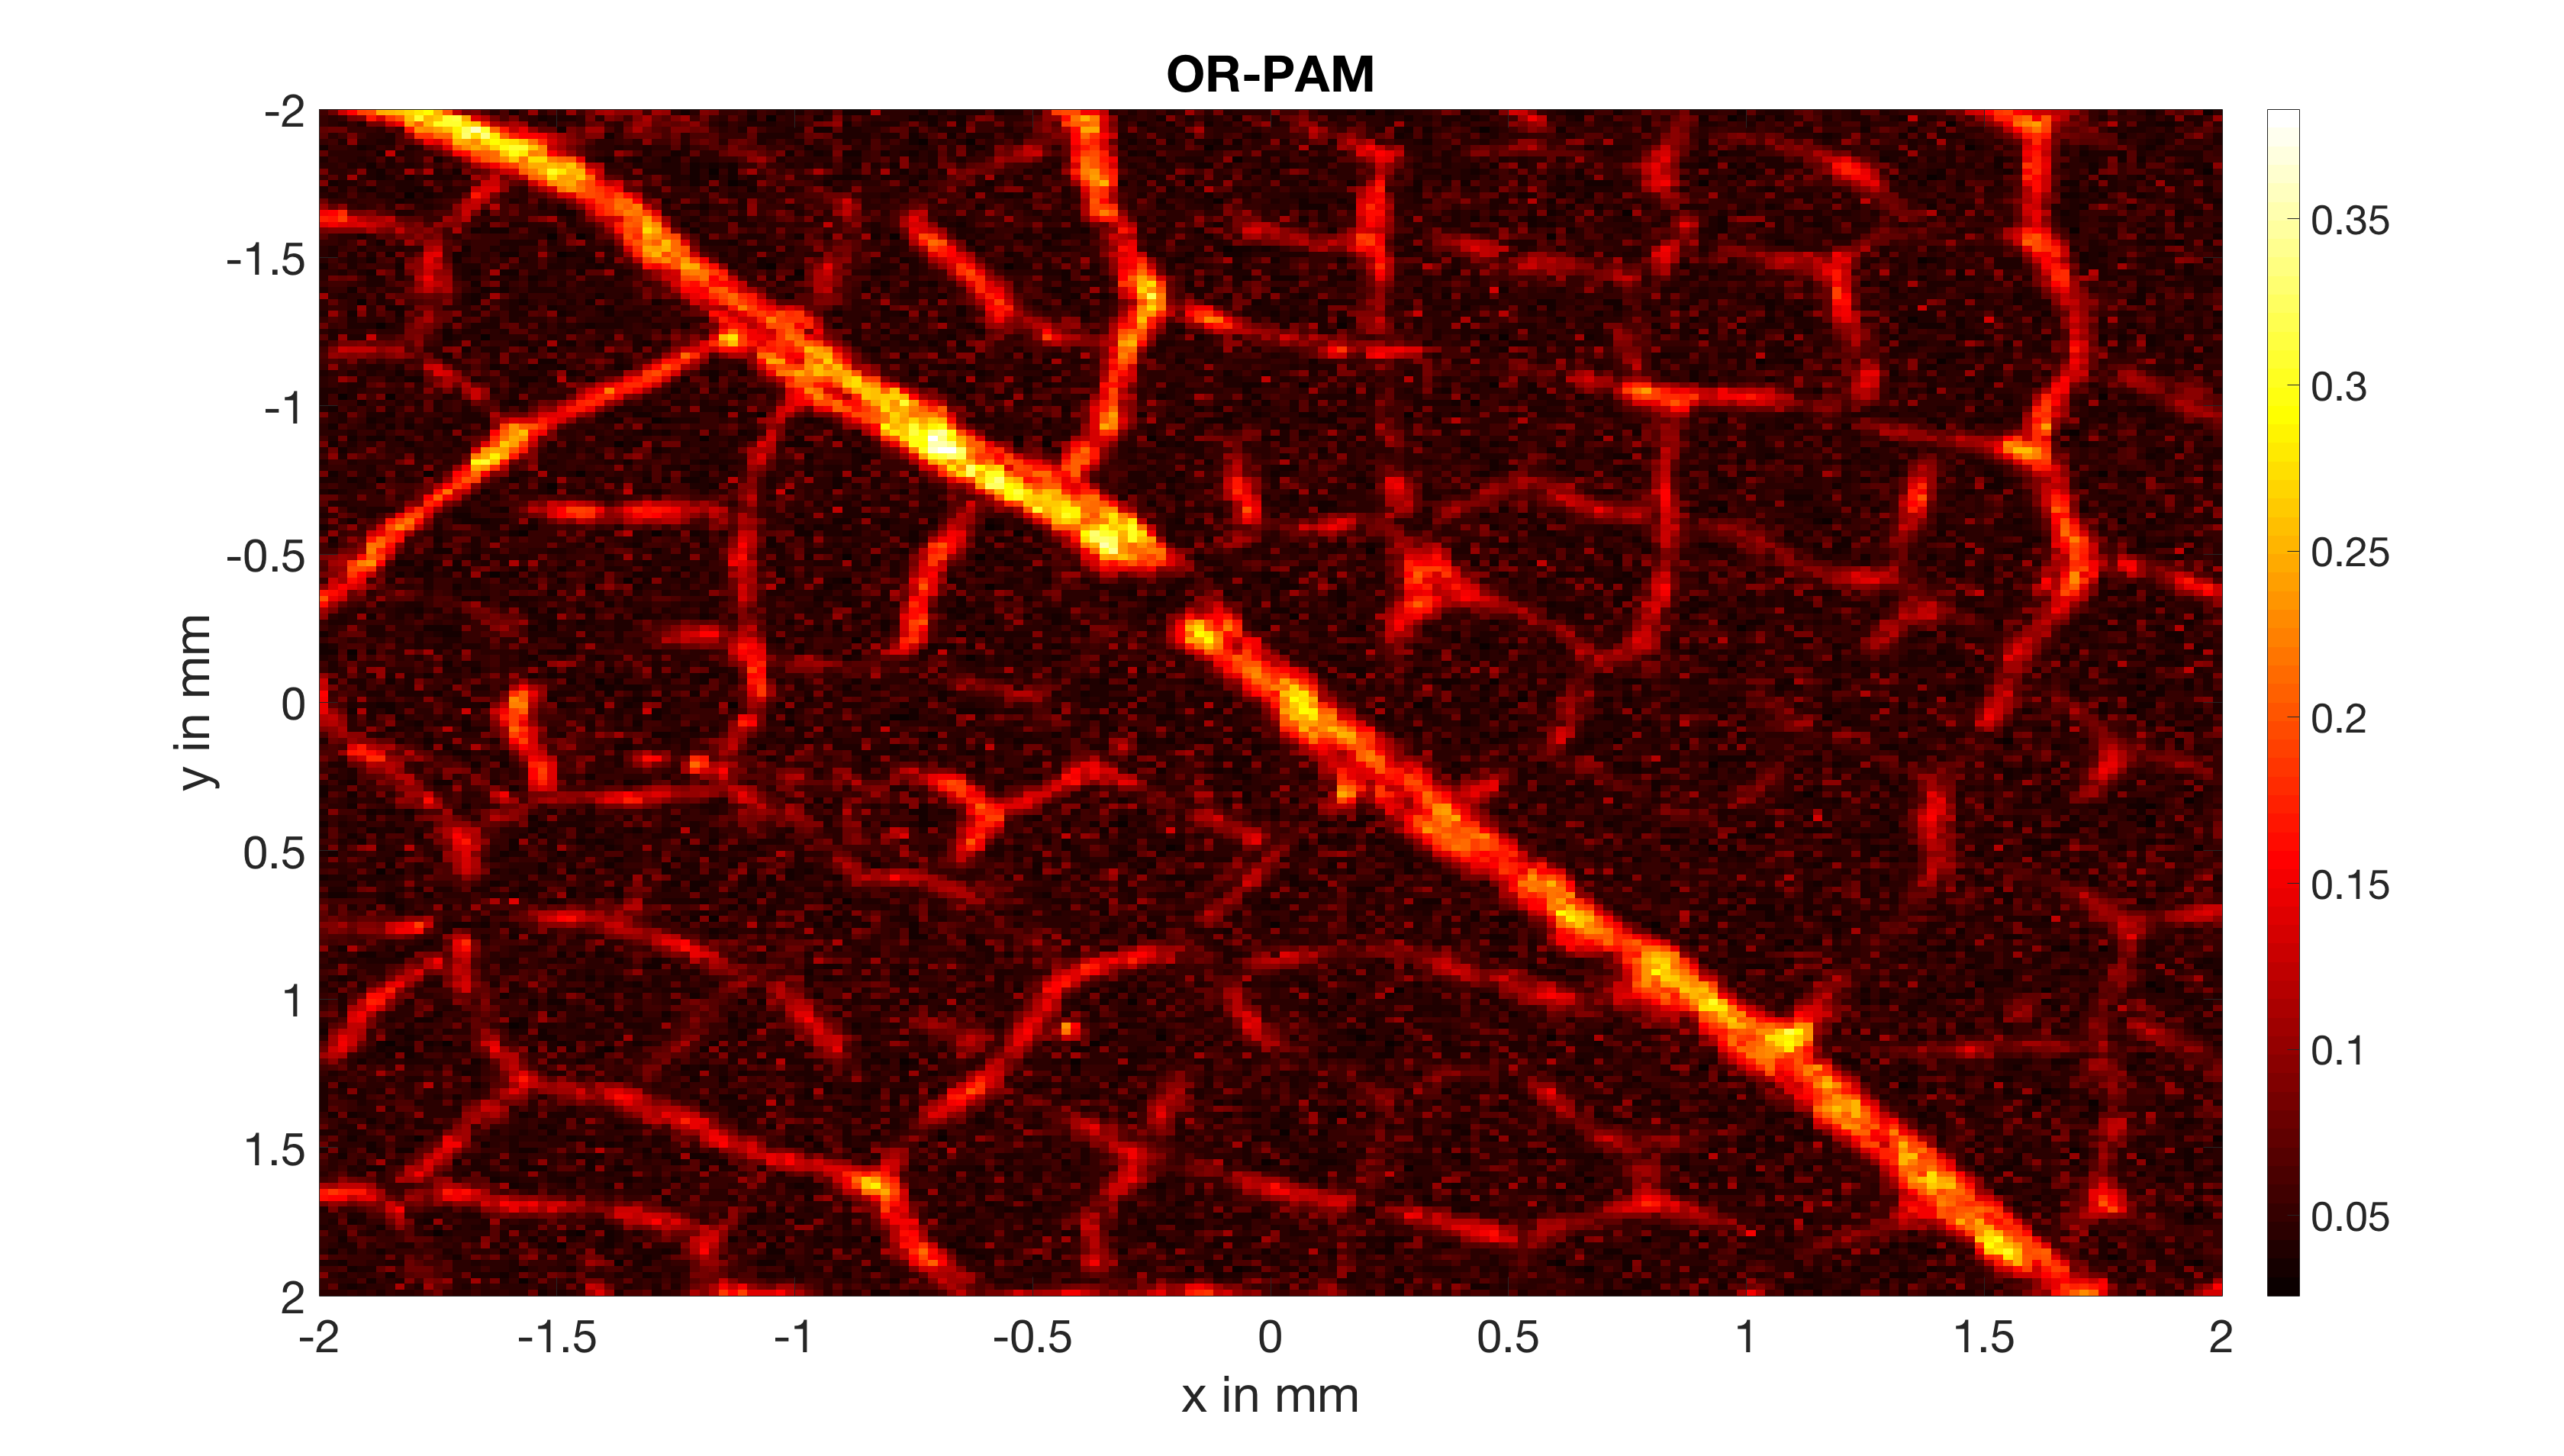
\includegraphics[width = 0.8\textwidth, height=0.38\textheight]{04_ex-results_of_PAM/images/blackleaf_OR.png}
	\end{minipage}	
	b)
	\begin{minipage}{\textwidth}
		\centering		
		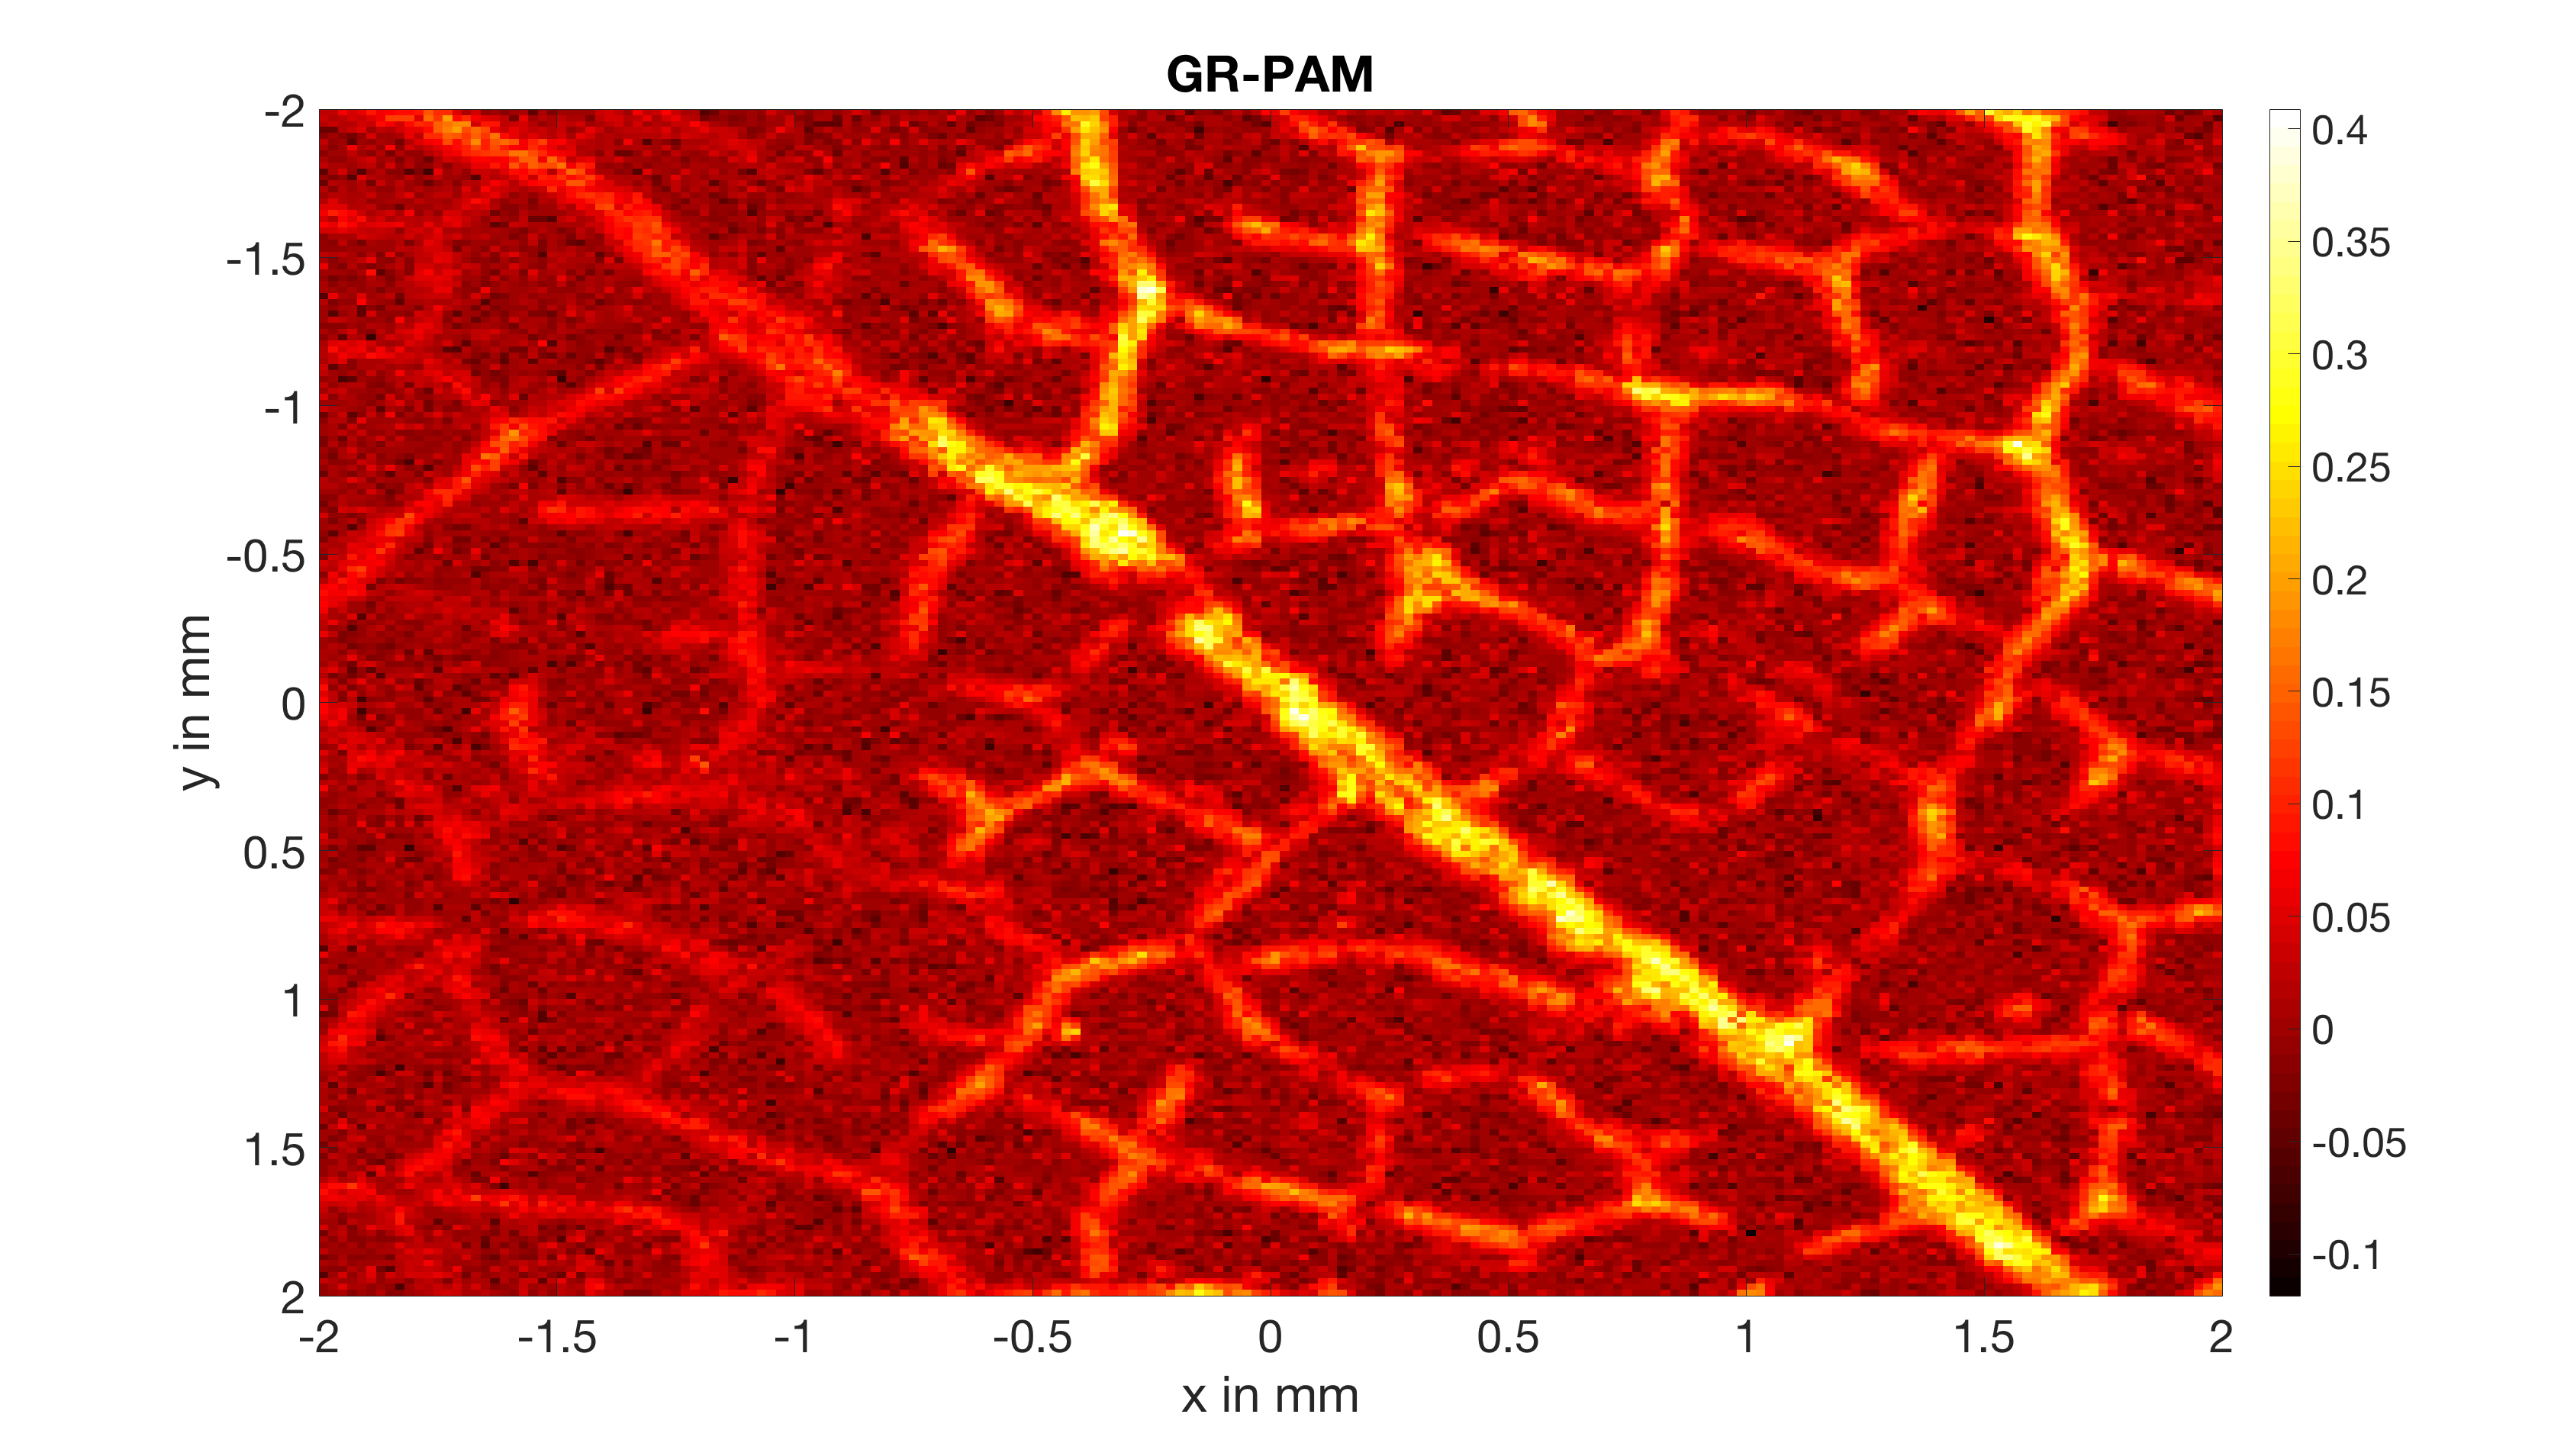
\includegraphics[width = 0.8\textwidth, height=0.38\textheight]{04_ex-results_of_PAM/images/blackleaf_GR.png}
	\end{minipage}
	
	\caption{Image of a black plastic leaf. The scan area is 4 x 4~$mm$ with 200 points and a step size of 20~$\mu m$ taken in each direction.}
	\label{fig:imgGRblackleaf}
\end{figure}

In figure \ref{fig:imgGRblackleaf} a) a conventional OR-PAM picture is shown. Furthermore, \ref{fig:imgGRblackleaf} b) shows a GR-PAM image. It is visible, that in \ref{fig:imgGRblackleaf} b), the left part and some of the ramification is weaker than the others, whereas the main strand appears mostly exceedingly. This can be assigned towards the sectioning capabilities of GR-PAM. 

\subsubsection{Lateral resolution determination}

To determine the resolution of the photoacoustic measurements a resolution target (Edmund Optics, USAF 1951) were scanned. \\
The resolution of an optical system can be found by scanning over a sharp edge, giving a edge spread function (ESF). The derivation of the ESF produces a Gaussian shaped function. Thereby the FWHM can be built, which results the resolution.\\

 \begin{figure}[H]
 	a)
 	\begin{minipage}{0.5\textwidth}		
 		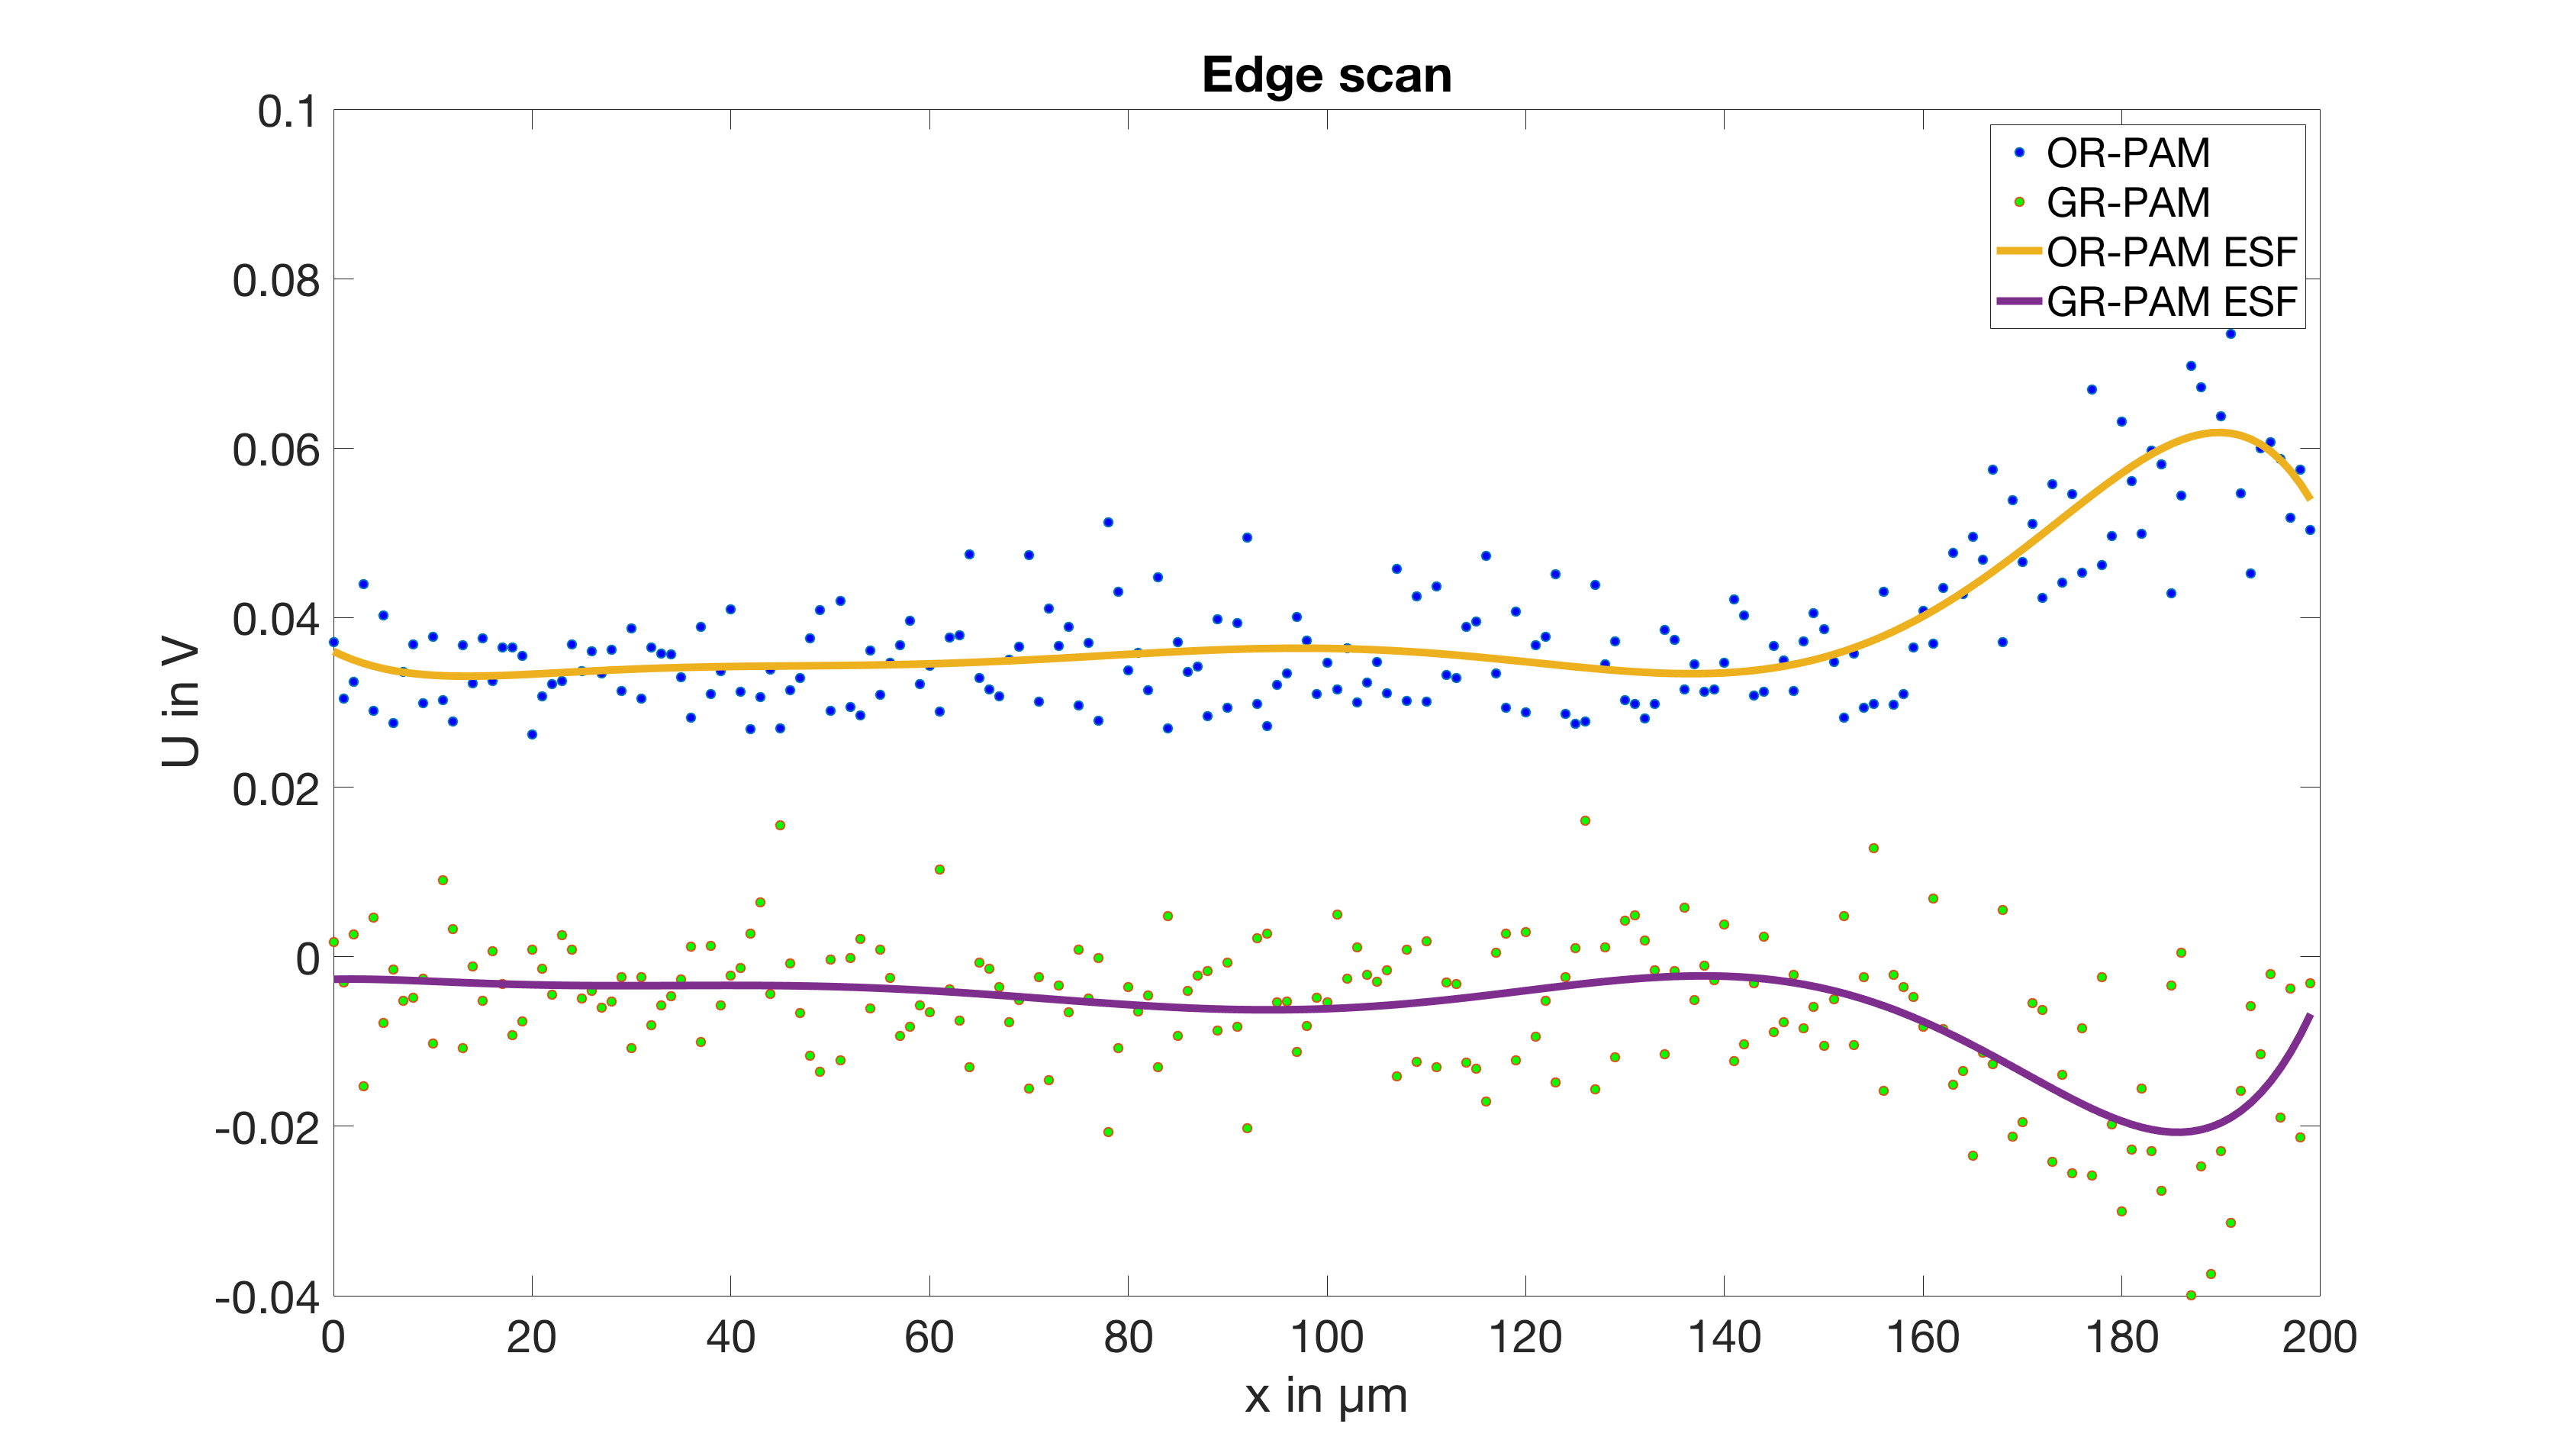
\includegraphics[width = \textwidth, height=0.25\textheight]{04_ex-results_of_PAM/images/ESF.png}
 	\end{minipage}	
 	b)
 	\begin{minipage}{0.5\textwidth}		
 		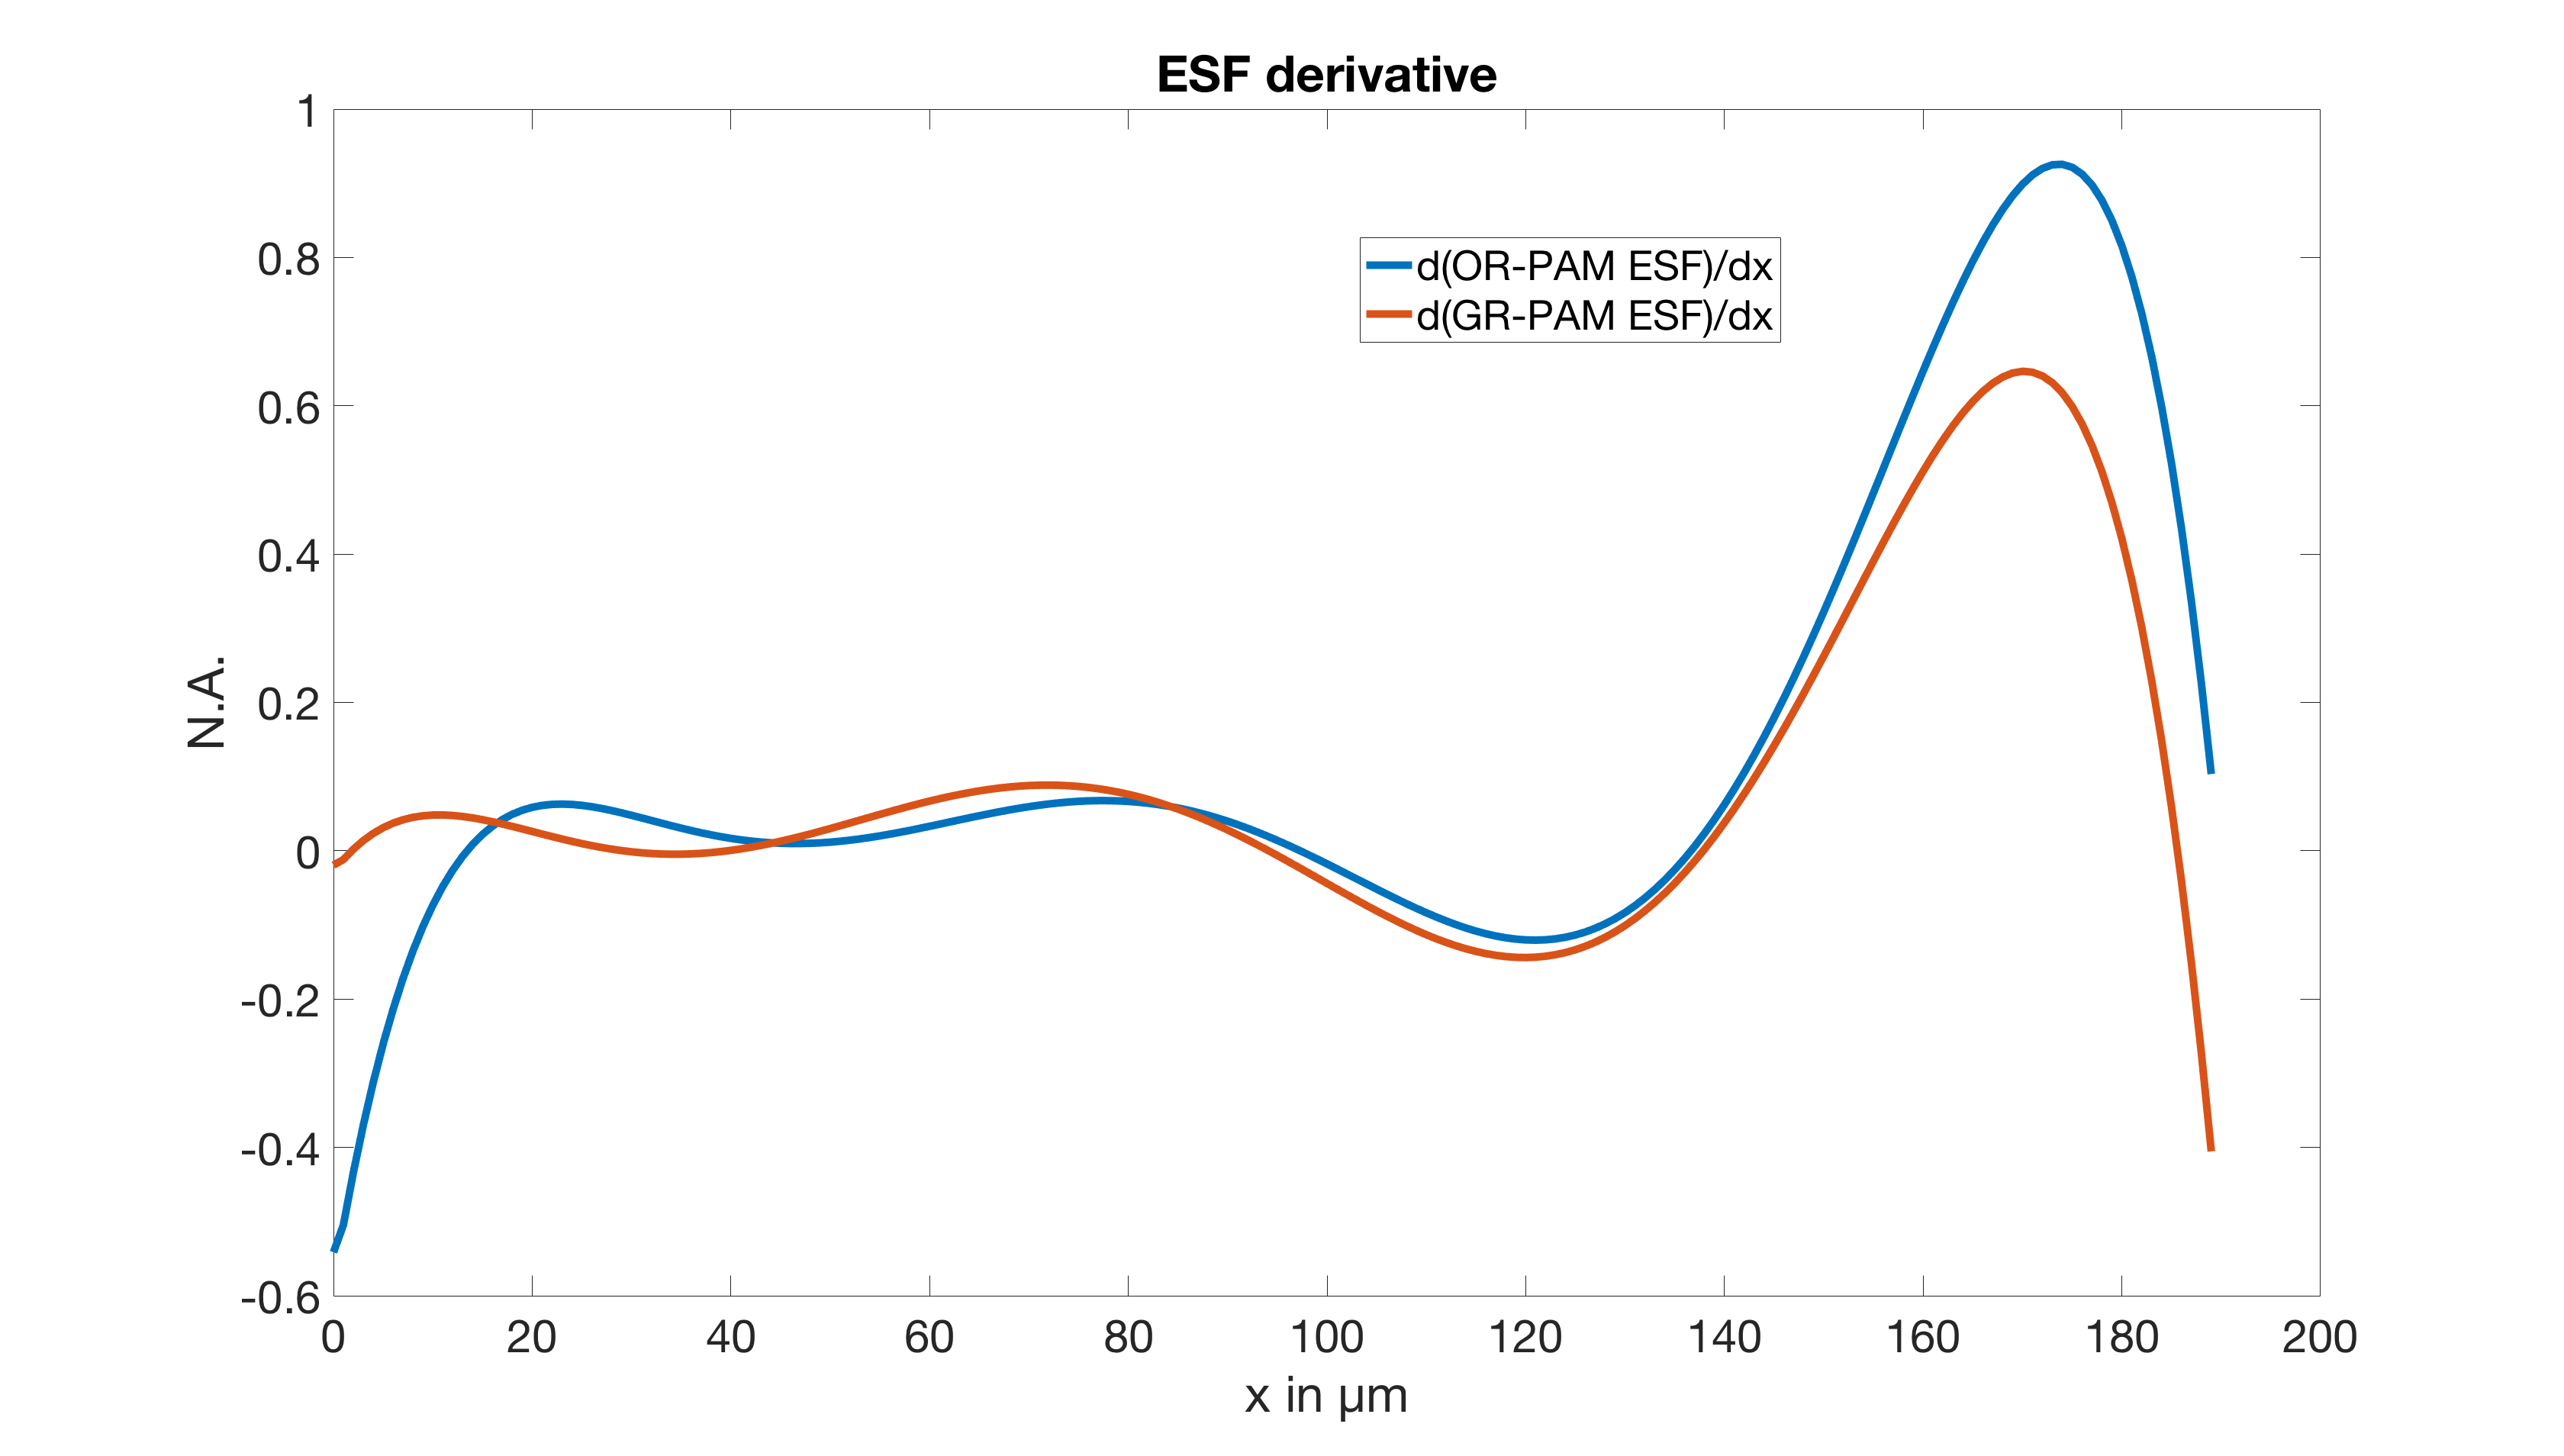
\includegraphics[width = \textwidth, height=0.25\textheight]{04_ex-results_of_PAM/images/ESFderivative.png}
 	\end{minipage}
 	
 	\caption{In a) the measured data points of the scan over an edge are displayed. These are fitted by an polynomial fit of order 9, which is the ESF. Figure b) shows the derivative of the fit function. Here 200 datapoints are taken at a 1$\mu m$ increment.}
 	\label{fig:ESF}
 \end{figure}

Figure \ref{fig:ESF} shows a measurement and analysis of the investigated setup. The FWHM and therefore the resolution of OR-PAM is 31.3$\mu m$ and 29.3$\mu m$ for GR-PAM. Which is an improve of about 7$\%$. The value differs from the 41$\%$ calculated in \ref{sec:resConGR}. \\
A possible explanation for this discrepancy could be, that the change in $\Gamma$ occurs from the surrounding water and not from the resolution target. Because the elements of the resolution target are coated with chromium, which is a good heat conductor. Therefore the applied temperature change is transfered and stored in the water for the acoustic coupling. Furthermore, the chromium layer is very thin and the spherical pressure wave is generated on top of the chromium-water interface. This leads to an interference with the chromium-glass interface reflection.\\
To conclude, there is a measurable resolution improvement in GR-PAM, but the measurement should be done on an edge that contains an absorbing material with low heat conduction. 

\subsubsection{Thermal relaxation time}

The typical delay time between the two GR-PAM pulses in the measurements done before is 60~$\mu s$. The value is determined by trial and error and was completely practicable for the imaging tasks. \\
Therefore it become apparent to investigate in the thermal relaxation time of water, as water is the coupling media and main constituent in the used specimen. \\
In figure \ref{fig:thermalRelaxTime} the amplitude increase due to the Grueneisen effect is displayed in percent over the delaytime between the pulses.

\begin{figure}[H]
	\centering
	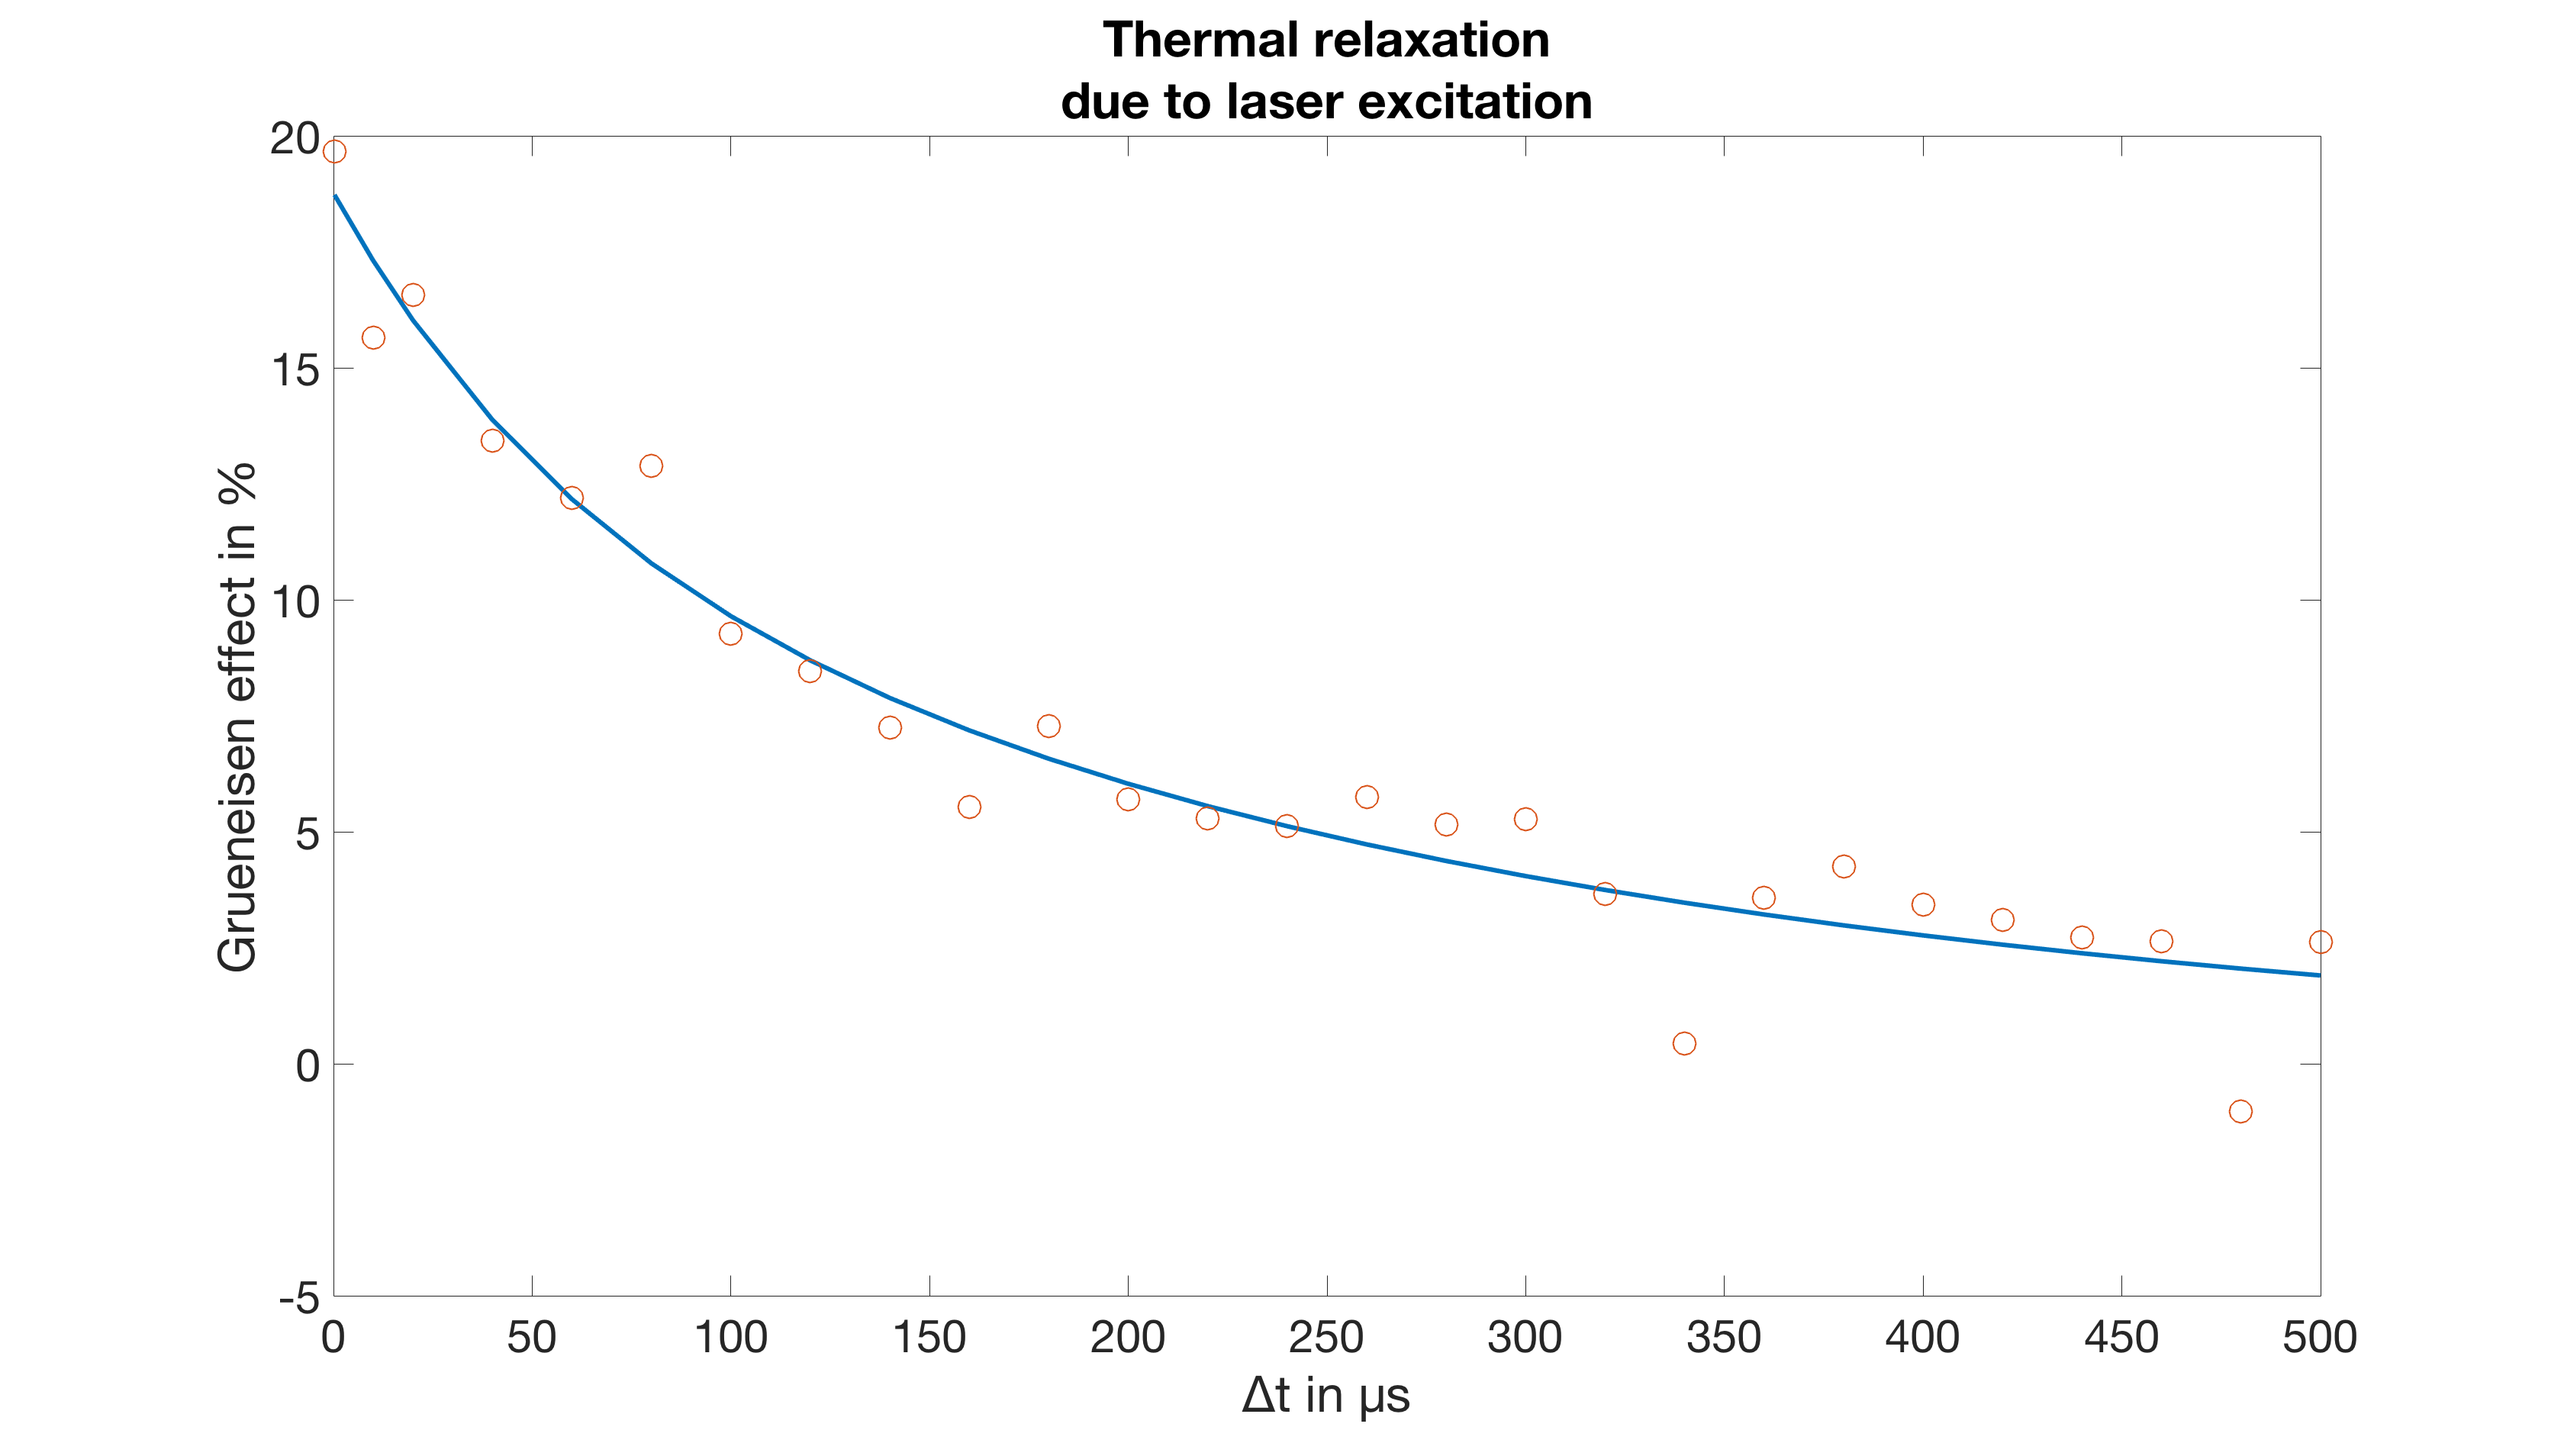
\includegraphics[ height=0.35\textheight]{04_ex-results_of_PAM/images/thermalRelaxTime.png}
	\caption{The dependency of the Grueneisen effect on the delay time between heating and detection laser pulse, for OrangeG colored water. The fitted curve parameter for the relaxation time is $\tau_{water}$ = 270.27~$\mu s$}
	\label{fig:thermalRelaxTime}
\end{figure}

It can be seen that the Grueneisen effect declines as the delay time increases. \\
Also the taken value of 60~$\mu s$ generates in the OrangeG colored water a Grueneisen effect of about 12~$\%$. Therefore the estimated value is suitable for the measurements. 

\subsection{Topographical analysis of OR-PAM images}
\label{sec:topoPAI}

The 3D data cube, described in section \ref{sec:DAQ}, produced by OR-PAM, can be used to map topographical properties.\\
Figure \ref{fig:blackleaf3D} shows a example for such a data volume.

\begin{figure}[H]
	\centering
	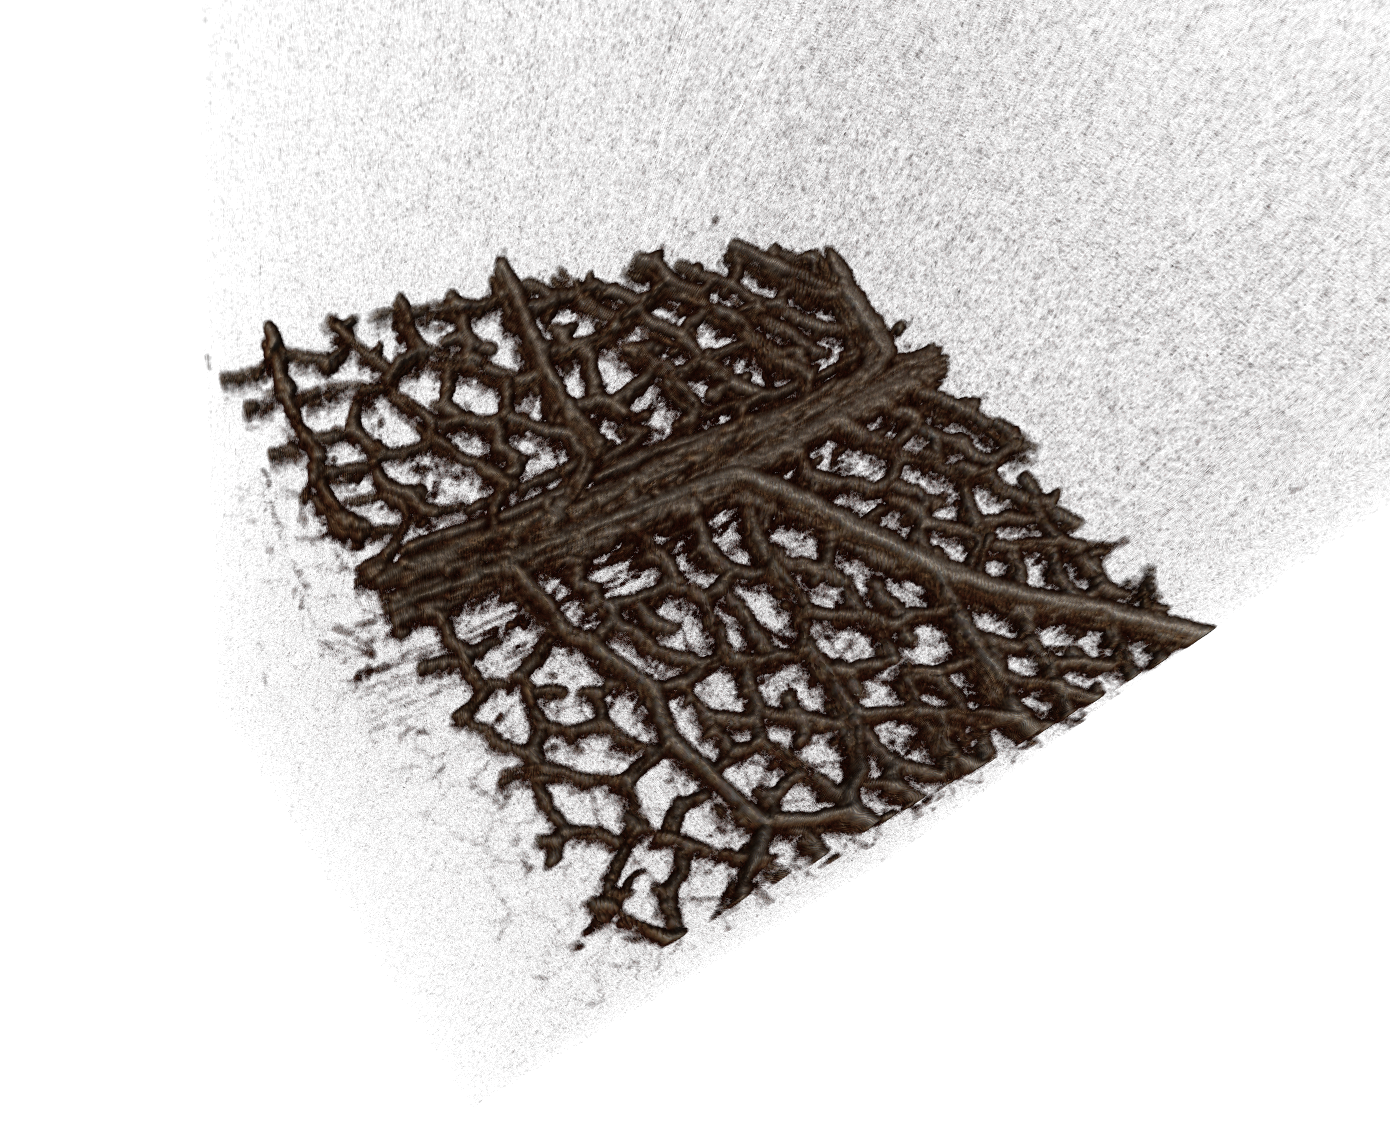
\includegraphics[ height=0.35\textheight]{04_ex-results_of_PAM/images/OR_PAM3G.png}
	\caption{3D image of a black leaf sample. The image size is 8 x 8~$mm$, there the step size is 40~$\mu m$ and 200 steps in each direction.}
	\label{fig:blackleaf3D}
\end{figure}

The sample were a black plastic leaf, which has good absorption properties at the used laser excitation wavelength of 527~$nm$. The dark shadows below the maximum amplitude plane are reflexions from the downside of the leaf and the sample carrier.\\
The structure of the leaf is clearly visible, moreover, the difference in height between the smaller ramification and the main strand. Therefore, the runtime of the ultrasonic waves can be interpreted to gain topographical images of surfaces. This analysis method is applicable to every material where the photoacoustic effect is achievable.\\
Figure \ref{fig:coin3D} shows the 3D image of a coin. 

\begin{figure}[H]
	\centering
		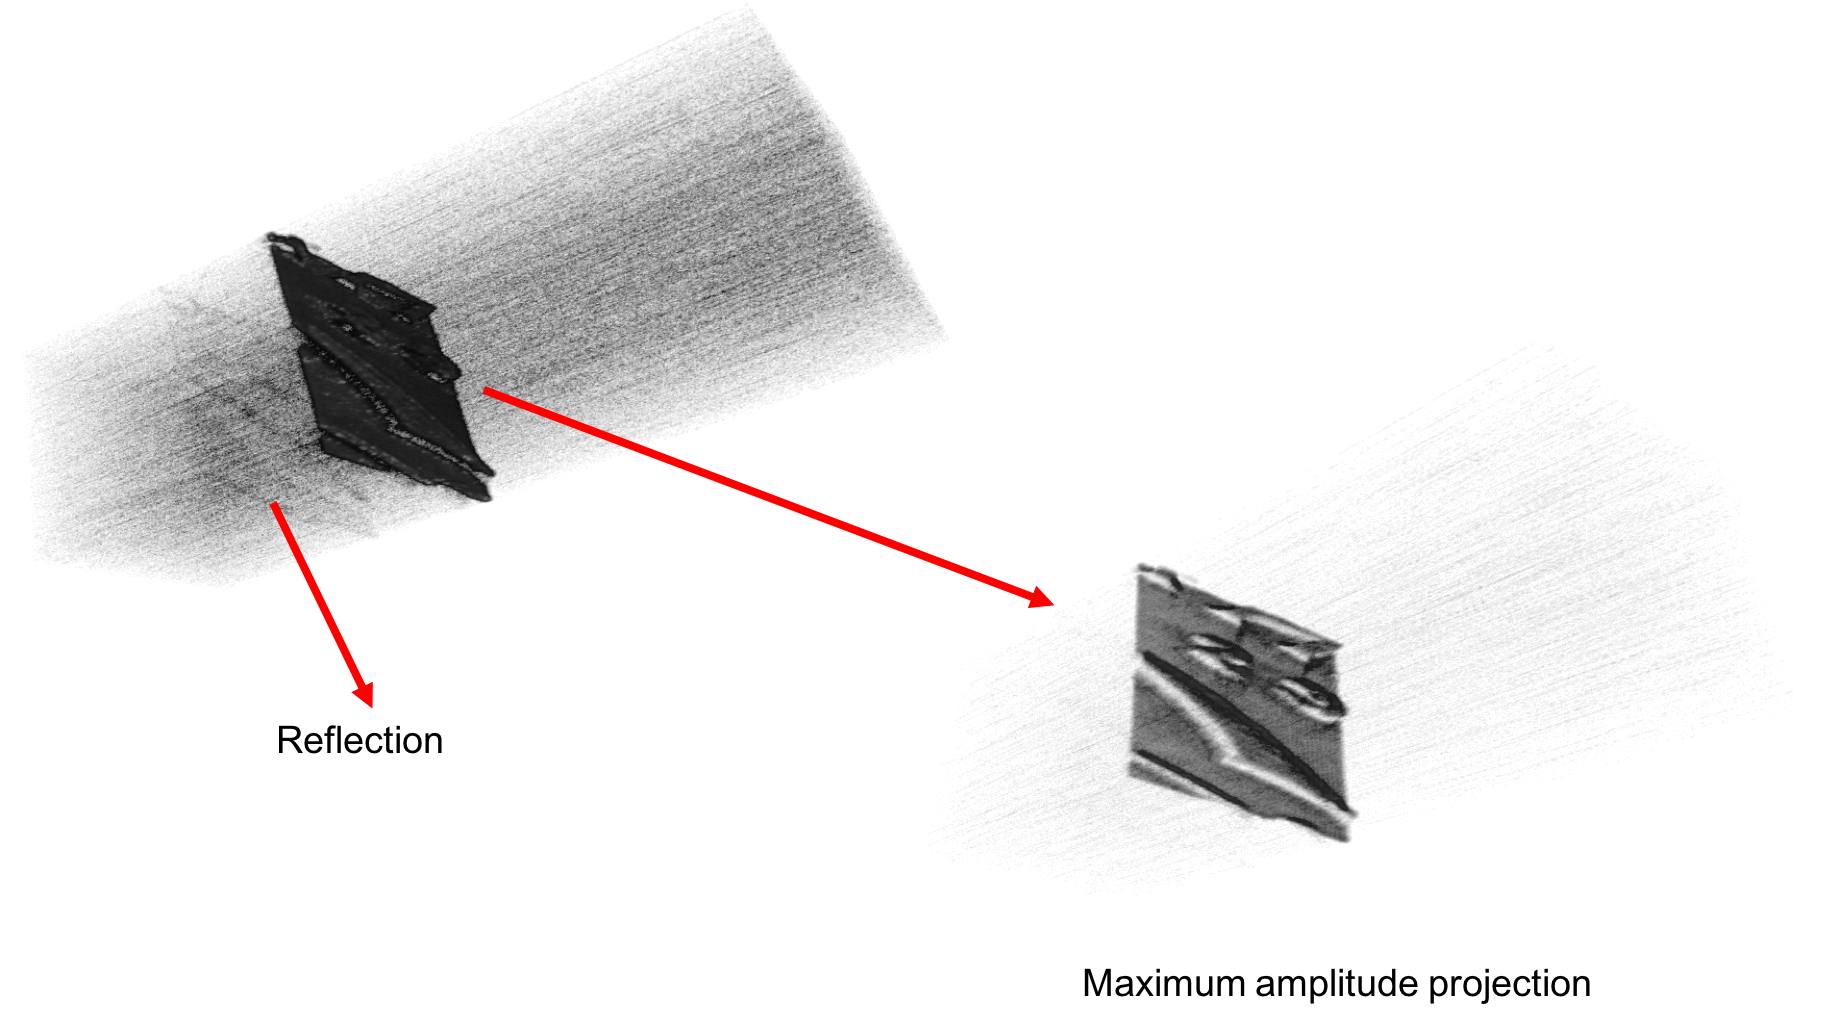
\includegraphics[width = 0.75\textwidth, height=0.28\textheight]{04_ex-results_of_PAM/images/coin3Dzoom.jpg}
	\caption{3D information block of a coin. The image size is 8 x 8~$mm$, there the step size is 40~$\mu m$ and 200 steps in each direction.}
	\label{fig:coin3D}
\end{figure}

Additional to the determination of topographical properties the backside- and other reflections can be used to determine layer thickness of the sample or its quality. \\
Another property that can be determined is the sample tilt in respect to the scan plane. Thus figure \ref{fig:sampletilt} shows the comparison between the maximum amplitude and runtime around a average value, taken from the black leaf data volume shown in figure \ref{fig:blackleaf3D}. The heatmap for the runtime is converted into length scale. 

\begin{figure}[H]
	\centering
	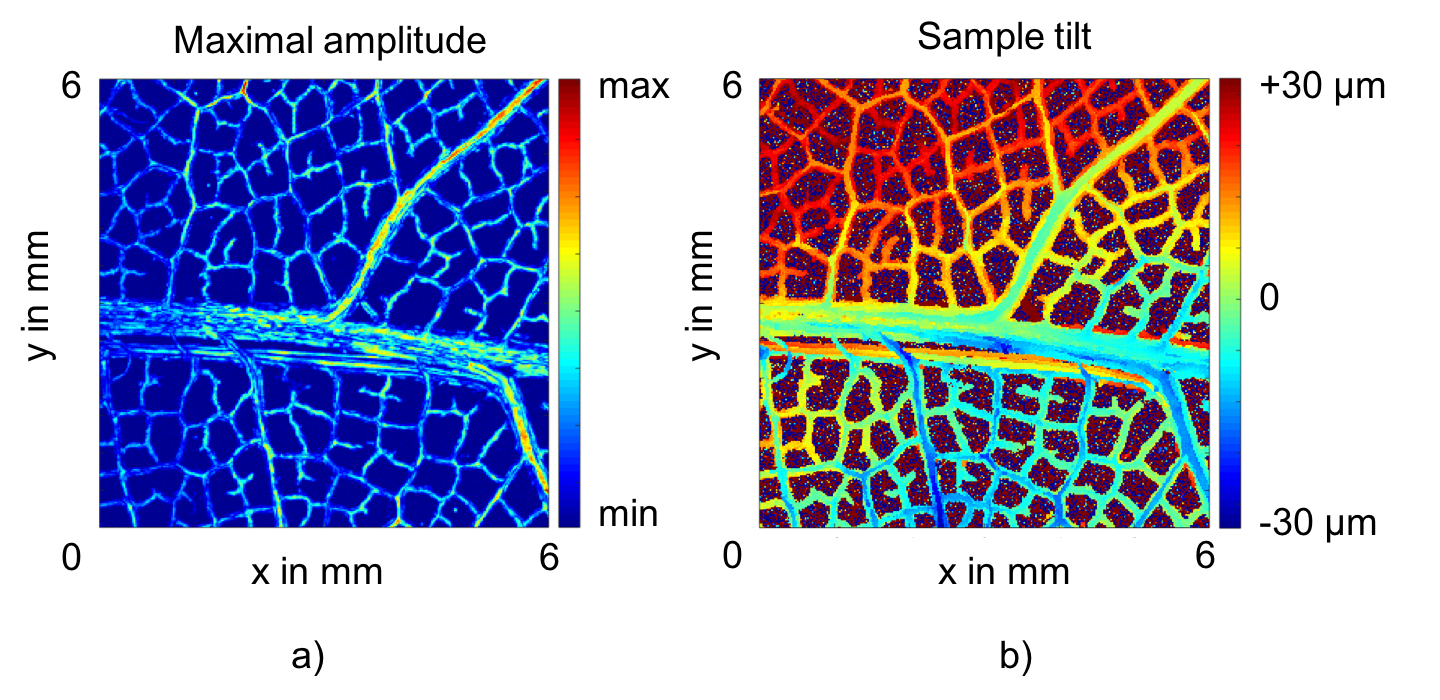
\includegraphics[ width = 0.95\textwidth, height=0.3\textheight]{04_ex-results_of_PAM/images/sampletilt.jpg}
	\caption{In a) the maximum amplitude from the black leaf data set is taken and b) shows a runtime analysis.}
	\label{fig:sampletilt}
\end{figure}

The red shaded area in figure \ref{fig:sampletilt} b) is the part where the ultrasonic signal arrived earlier than in the blue shaded parts. Therefore the upper left corner is closer to the scan plane than the lower right corner. This corresponds to a tilt of the sample. 



\section{Optical ultrasonic detection (OUSD)}
\label{sec:OUSD}
The requirements towards the setups in photoacoustic microscopy, shown in figure \ref{fig:ORPAMsetup}, have in common that the ultrasonic transducer has to be placed as close as possible to the origin of the ultrasonic wave. In order to achieve such configurations it is necessary to drill holes through the piezo-electric transducer or bypass the ultrasonic wave or excitation light to minimize the loss of information. Another approach to this topic is to use light, to detect ultrasonic waves and therefore combine optical and acoustical pathways. 

\subsection{Principle of optical ultrasonic detection}

The approach is based on a Fabry–P\'{e}rot interferometer (FPI). In a FPI light is applied onto two partially transmitting mirrors, which are placed parallel to each other. This setup is called resonator because only wavelengths that meet a certain resonance condition are transmitted through it.\\
The operation principle of the FPI based OUSD is shown in figure \ref{fig:transmissionChange}. In order to get a measurable signal of  a pressure wave running through the resonator, a medium is placed between the mirrors, which changes its refractive index due to pressure. This leads to a variation of the resonance condition.

\begin{figure}[H]
	a)
	\begin{minipage}{0.5\textwidth}
		
		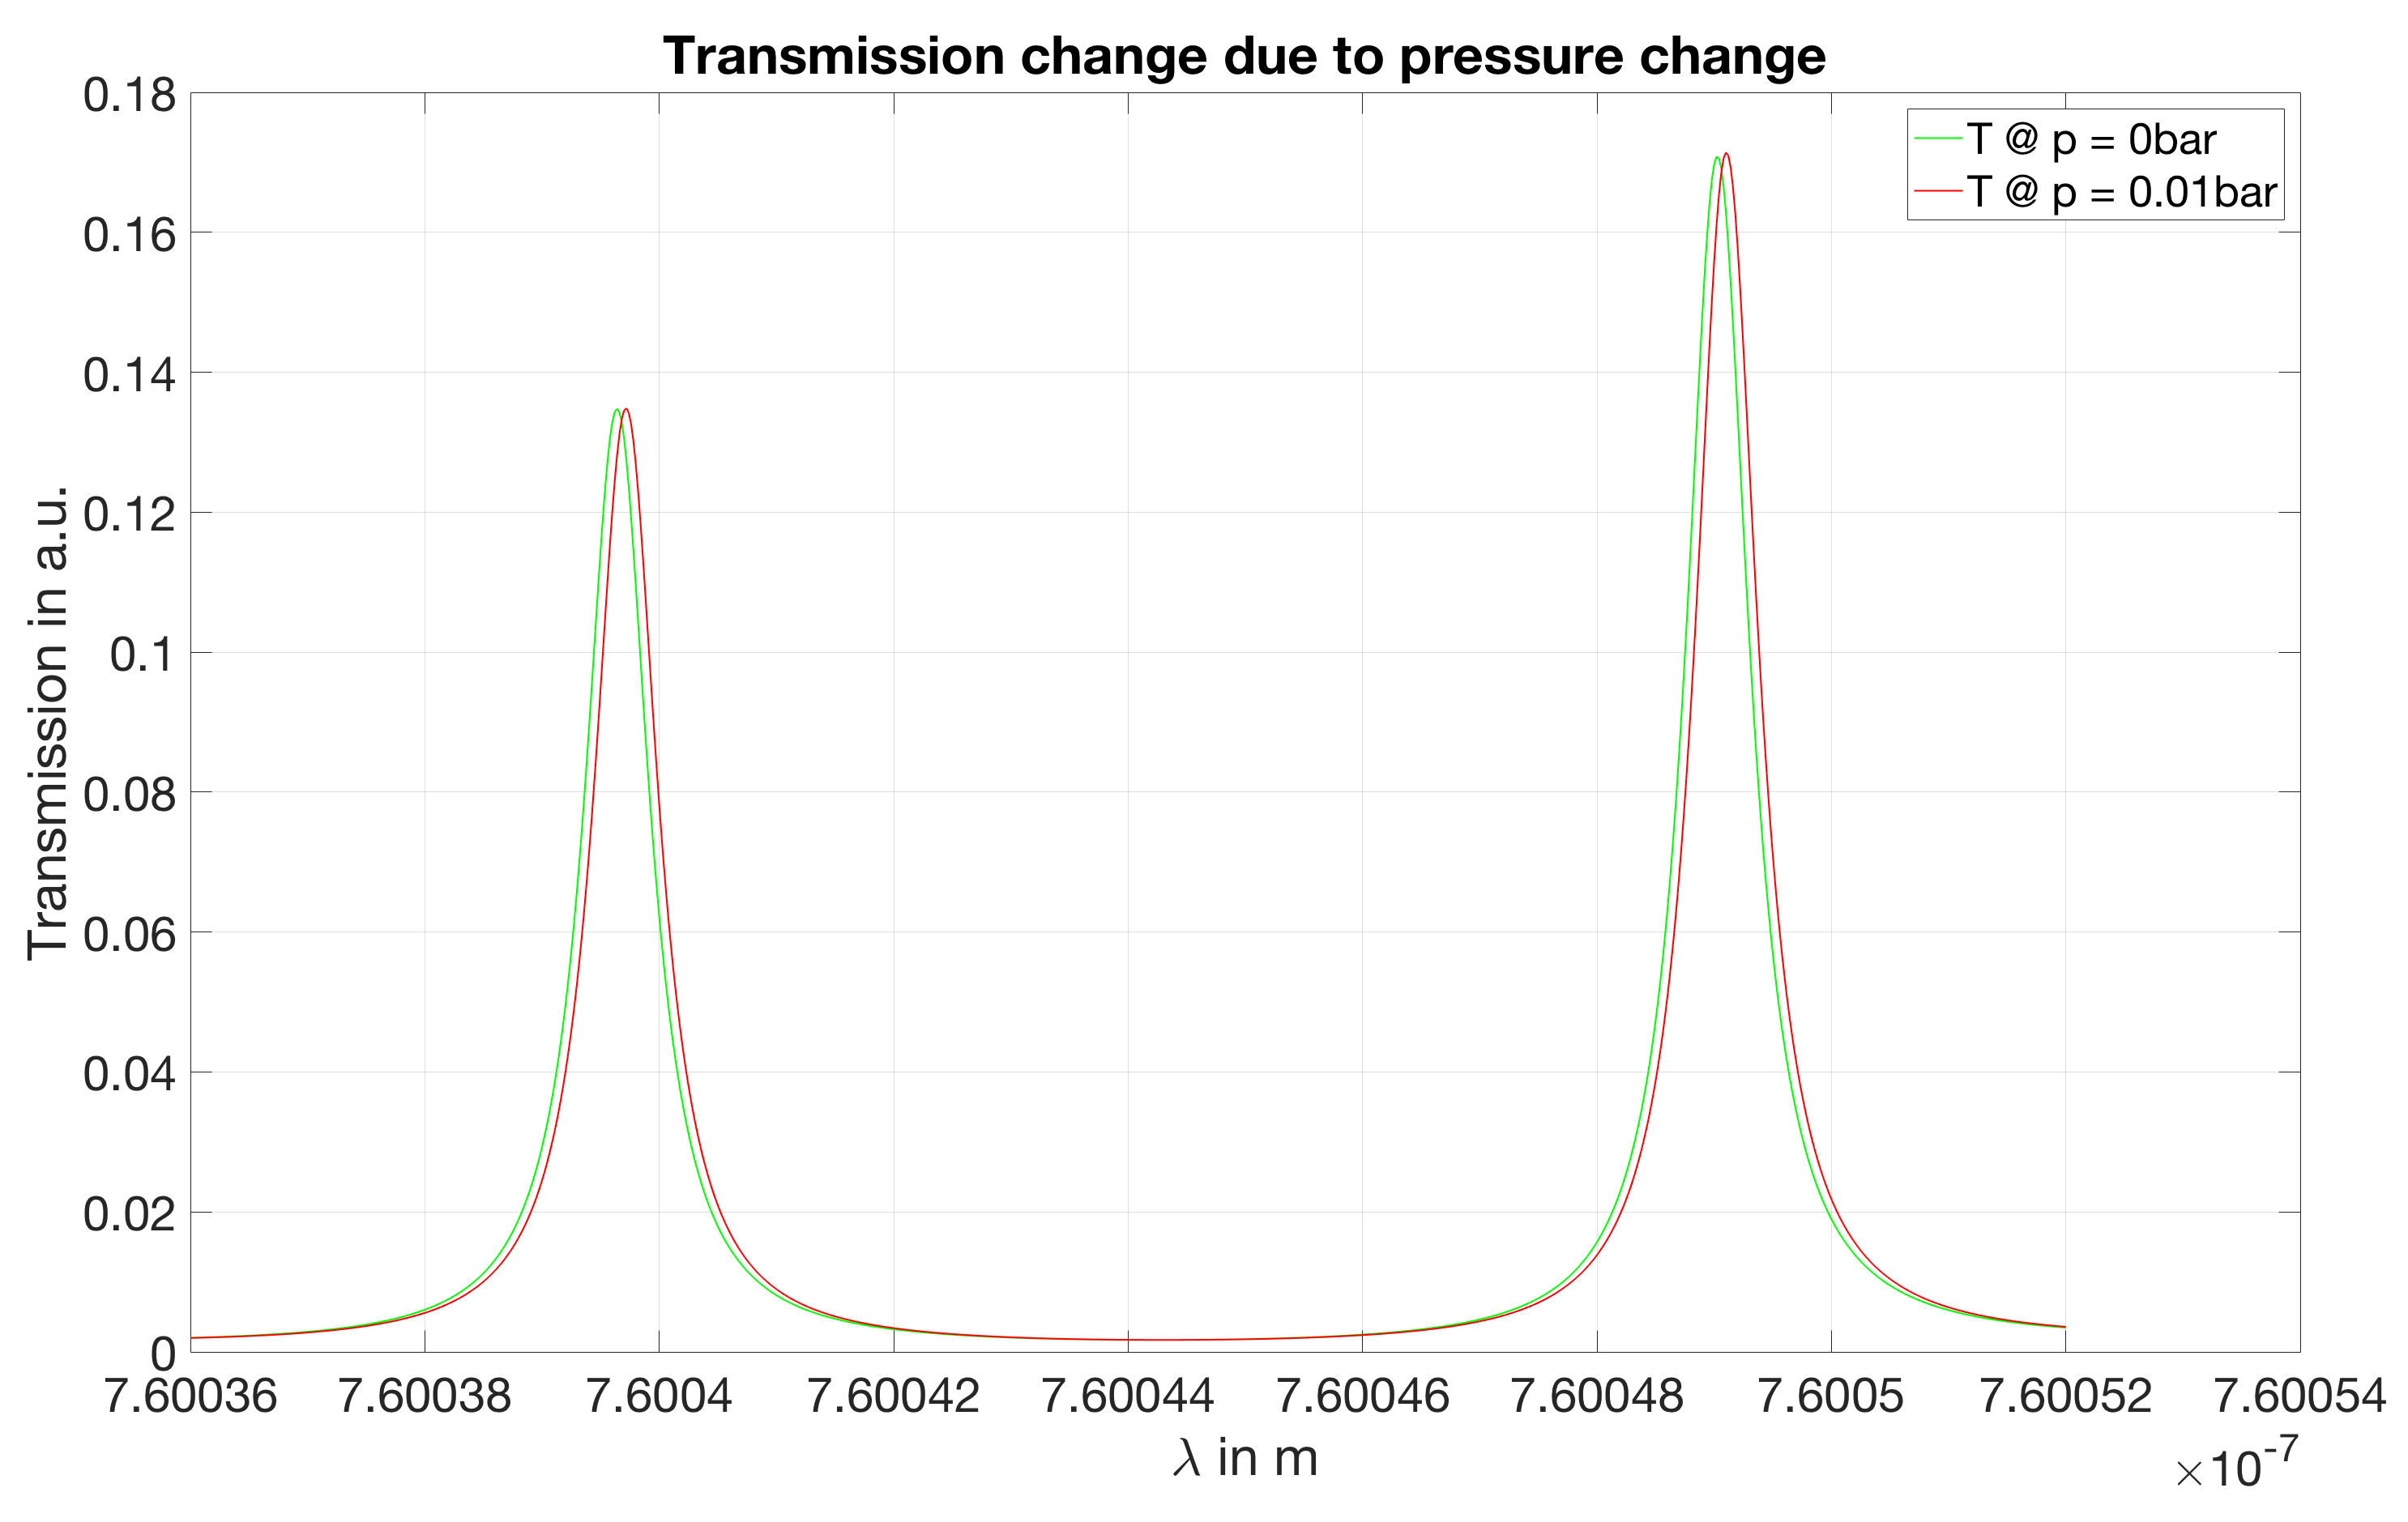
\includegraphics[width = \textwidth, height=0.3\textheight]{05_OUSD/images/transmissionChangePressure.png}
	\end{minipage}
	b)
	\begin{minipage}{0.5\textwidth}
		
		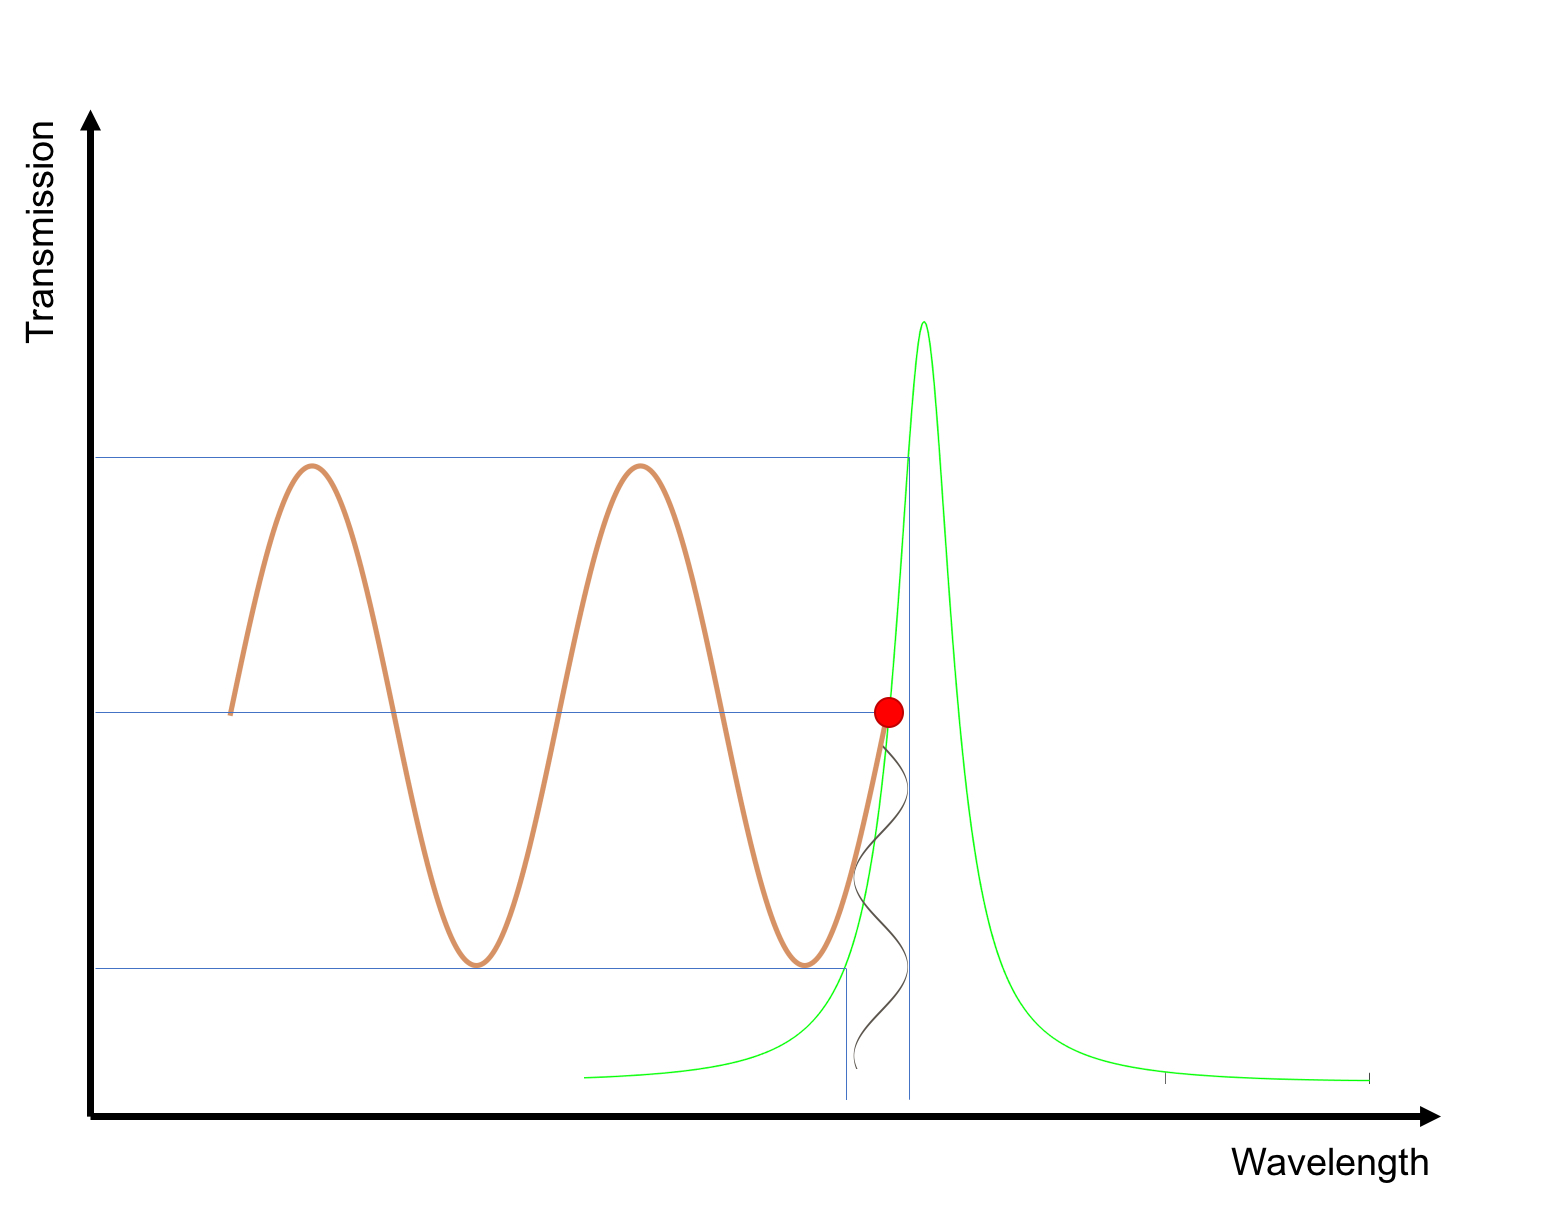
\includegraphics[width = \textwidth, height=0.35\textheight]{05_OUSD/images/sigSchematic.jpg}
	\end{minipage}
	
	\caption{a) shows how a pressure change influences the transmission condition of the resonator and in b) the response of the system to an incoming sinusoidal pressure wave is shown.}
	\label{fig:transmissionChange}
\end{figure}
 
Therefore figure \ref{fig:transmissionChange} a) shows a simulated transmission pattern at ambient pressure (green line) and at a constant pressure higher than the ambient pressure. The chosen pressure level is higher than a typical photoacoustic amplitude (red line), to better illustrate the effect. Thus, a shift towards longer wavelengths in the transmission pattern, can be seen. The simulation were done with water as a medium between the mirrors and its elasto-optic coupling coefficient $\frac{\mathrm{d}n}{\mathrm{d}p} = 1.35\; \mathrm{x} \;10^{-5} bar^{-1}$.\\
In figure \ref{fig:transmissionChange} b) the response to an incoming sinusoidal pressure change is shown. The system is regulated to hold its working point at a wavelength, there the transmission gradient (highlighted by the red point) has its maximum at ambient pressure. In order to keep this point stable the system is adjusted in a way that environmental stress is eliminated. But if a pressure wave in the $MHz$ range hits the resonator system the control is to slow to react and the red point moves as the transmission pattern moves, as shown in figure \ref{fig:transmissionChange} b). This leads to a change in the light intensity, which leaves the resonator. A photodetector that is placed behind the FPI converts the light into a voltage signal. 

\subsection{OUSD setup}

As shown in figure \ref{fig:FPIschematic} an induced ultrasonic wave travels back the optical path and interferes with the media between the two partially transmitting mirrors. The chosen medium were water, because its cheap and durable. The other feasibility would be FC77 an inert, dielectric liquid with higher $\frac{\mathrm{d}n}{\mathrm{d}p}$ than water, but because it volatilizes quickly, it is not suitable for longer measurements. 

\begin{figure}[H]
	\centering
	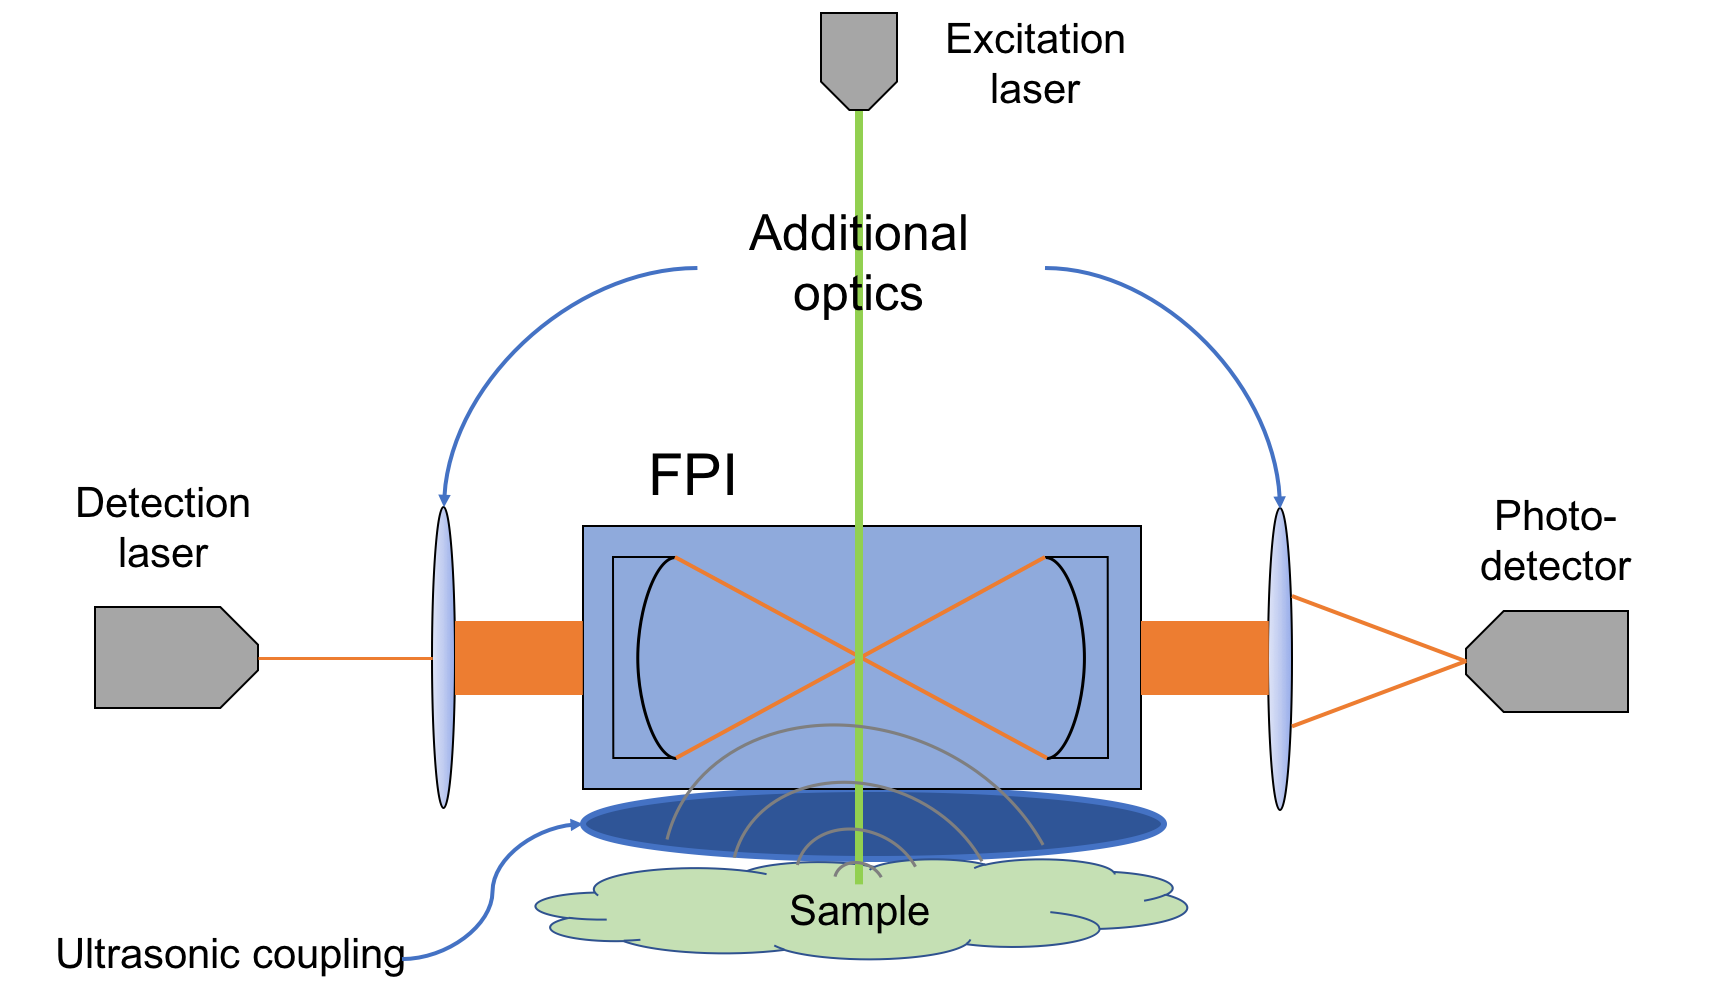
\includegraphics[height=0.4\textheight]{05_OUSD/images/FPIschematic.png}
	\caption{Schematic view of an optical ultrasonic detection system based on a Fabry–P\'{e}rot interferometer (FPI)}
	\label{fig:FPIschematic}
\end{figure} 

In order to make the system movable the detection laser and the excitation laser are brought to the system by optical fibers. The optics on the detection laser side consists of a bi-convex lens to collimate the beam and a plano-convex to focus it into the resonator. On the photodetector side a plano-convex lens focuses the transmitted light onto the photodiode. \\
The water of the resonator interior is restrained with the same transparent polymer membrane as in the OR-PAM setup.\\

\begin{figure}[H]
	a)
	\begin{minipage}{0.5\textwidth}
		
		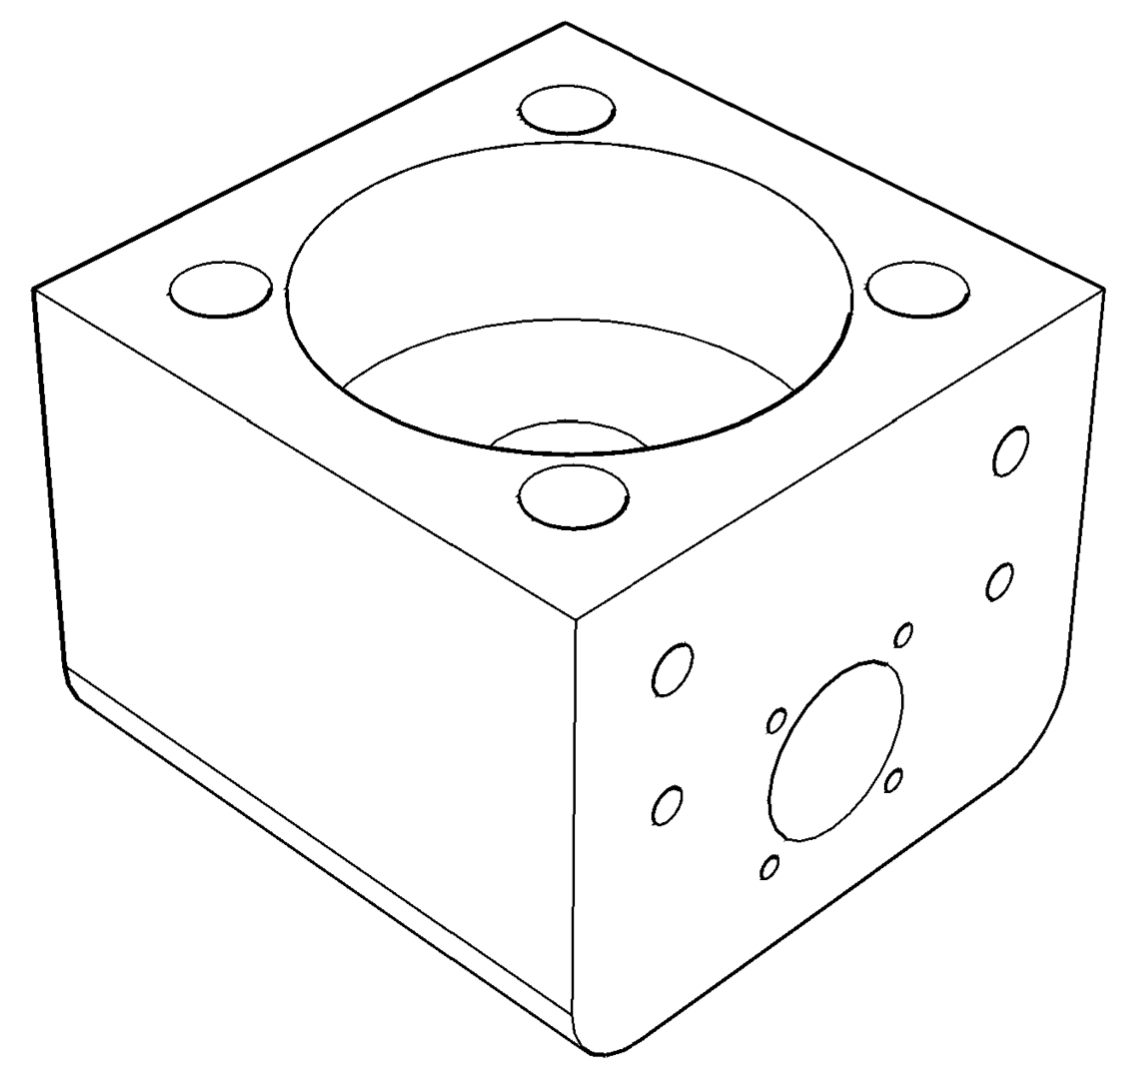
\includegraphics[width = \textwidth, height=0.35\textheight]{05_OUSD/images/res3D.jpg}
	\end{minipage}
	b)
	\begin{minipage}{0.5\textwidth}
		
		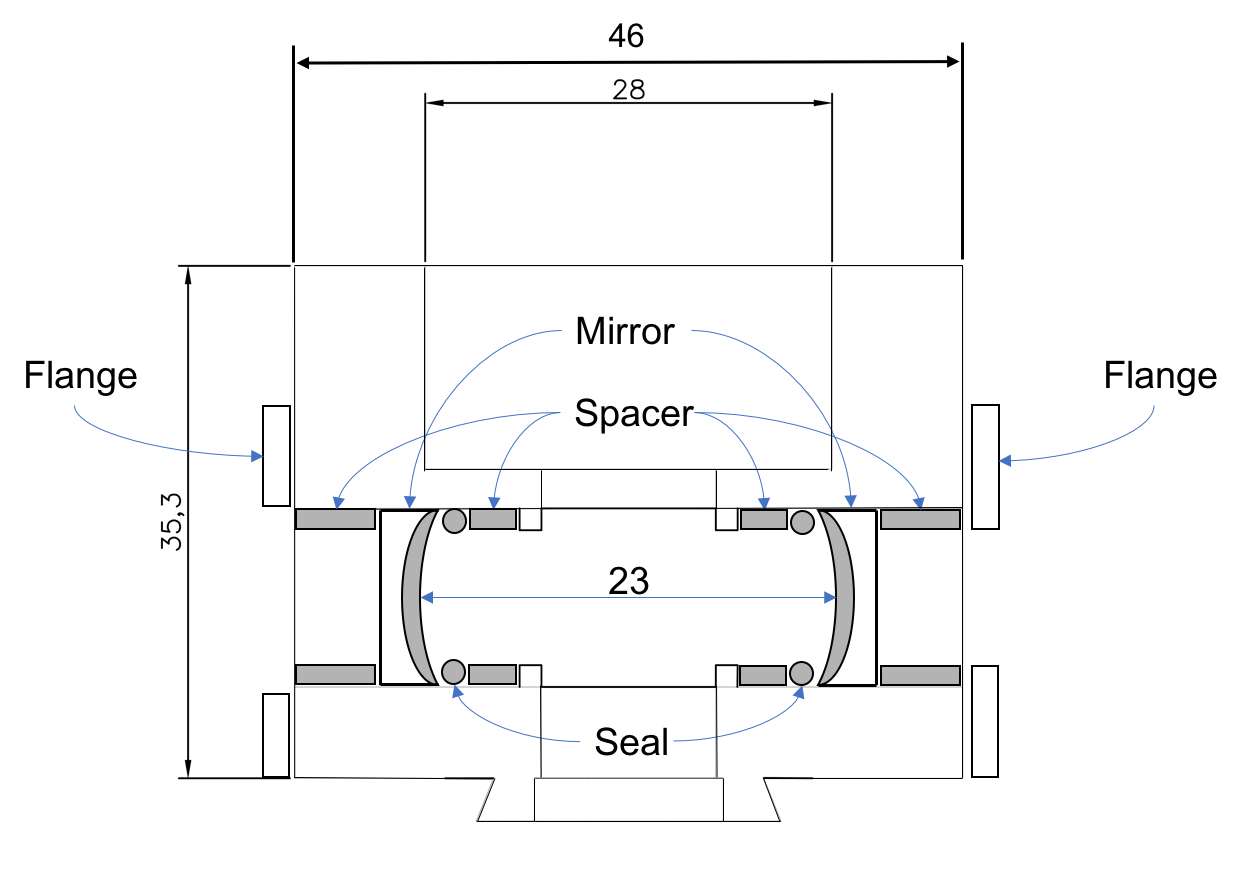
\includegraphics[width = \textwidth, height=0.3\textheight]{05_OUSD/images/resCut.jpg}
	\end{minipage}
	
	\caption{Schematic of the manufactured resonator. There a) shows a 3D model and b) a cut through it. All values are in $mm$.}
	\label{fig:resSchematic}
\end{figure}

Figure \ref{fig:resSchematic} b) shows a schematic cut through the resonator. The determination of the distance between mirrors gets discussed in section \ref{sec:resLength}. The flanges are pressing the mirrors against the spacers and seals to waterproof the system. Besides they are used to adjust the mirrors to match the focal points.\\
In figure Figure \ref{fig:resSchematic} a) a 3D model of the resonator is shown. The purpose of the holes in the front is to mount the flanges and the cage system. They also fix the cage system bars from the topside. There is also a hole on the topside to add an objective. \\

\subsection{System development}
\label{sec:sysDev}
This section shows the determination of the basic parameters of the resonator and mirrors. At first a resonator length is defined, followed by the simulation of the layer system that is coated onto the plane-concave lenses.\\
The system should be stable, but also have a maximum sensitivity for changes in the refractive index. Furthermore, the cutoff frequency should be as high as possible. 

\subsubsection{Resonator stability considerations}

There are several possibilities to setup a multi-beam interferometer, called resonator. For the specification of a stable system, a symmetrical ray profile and a minimum waist radius $w_0$. The waist radius can be written as

\begin{equation}
 w_0 = \left(\frac{\lambda L}{\pi}\right)^{1/2} \cdot \left(\frac{g_1 g_2(1-g_1g_2)}{(g_1 + g_2 - 2g_1g_2)^2}\right)^{1/4}
 \label{eq:w_0Res}
\end{equation}
\\
where $L$ is the resonator length, $\lambda$ the wavelength and $g_{1,2}$ are 

\begin{equation}
	g_{1,2} = 1-\frac{L}{R_{1,2}} 
	\label{eq:g1g2}
\end{equation}
\\
where $R_1$ and $R_2$ are the mirror radii \cite{eichler:laser}.  \\
Only configurations that meet the condition $0 \leq g_1 g_2 \leq 1$ are stable. Figure \ref{fig:resStability} shows all possible setups for a FPI. There only the blue shaded areas mark stable configurations.  

\begin{figure}[H]
	\centering
	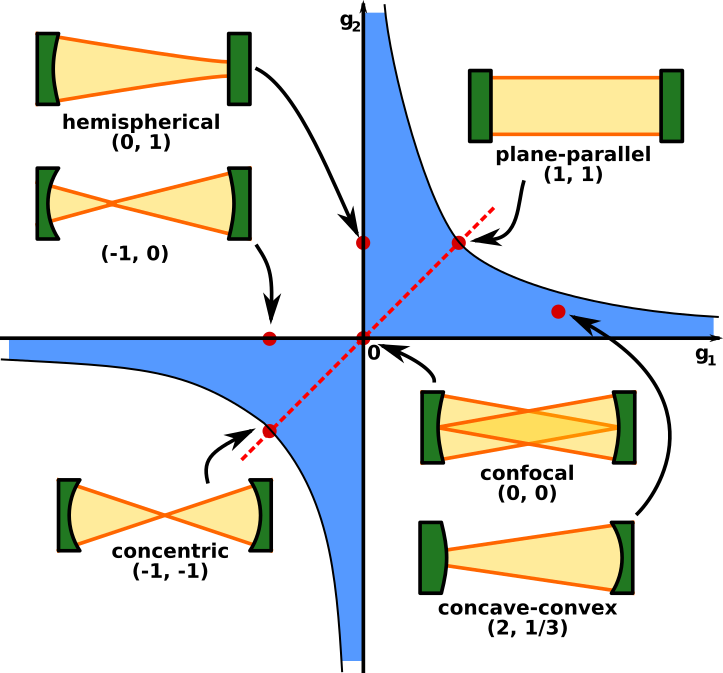
\includegraphics[height=0.4\textheight]{05_OUSD/images/Laser_resonator_stability.png}
	\caption{Resonator stability diagram for all possible arrangements of two mirrors. The blue shaded areas mark stable conditions, beyond them the system gets instable \cite{wiki:resStability}.}
	\label{fig:resStability}
\end{figure} 

In this case stable means that the light energy is located nearby the optical axis of the resonator and due to the finite mirror diameter, the diffraction losses are minimal. For unstable systems this means high diffraction losses \cite{eichler:laser}. 

\subsubsection{Resonator length determination}
\label{sec:resLength}
For the system, two plane concave mirrors from Edmund Optics (45016) with a diameter of 12~$mm$ and a radius of -12.40~$mm$, were chosen. Therefore the area of interest in figure \ref{fig:resStability} is the third quadrant. Thereby the mirrors are even so the red line marks all possible distance cases. The confocal case is the most stable one, but also with the least sensitivity. Vice versa the concentric case has the highest sensitivity, but is almost unstable.\\
Due to this conditions $g_1$ is equal $g_2$ and the formula for $w_0$ reduces to 

\begin{equation}
w_0 = \sqrt{\frac{\lambda}{2 \pi} \sqrt{L(2R-L)}}
\label{eq:w_0Reduced}
\end{equation}
\\
Figure \ref{fig:resLength} shows a simulation for the given mirror values. Also the wavelength were set to 760~$nm$, as this is the center frequency of the used tunable laser TEC 500 from Sacher Lasertechnik.

\begin{figure}[H]
	\centering
	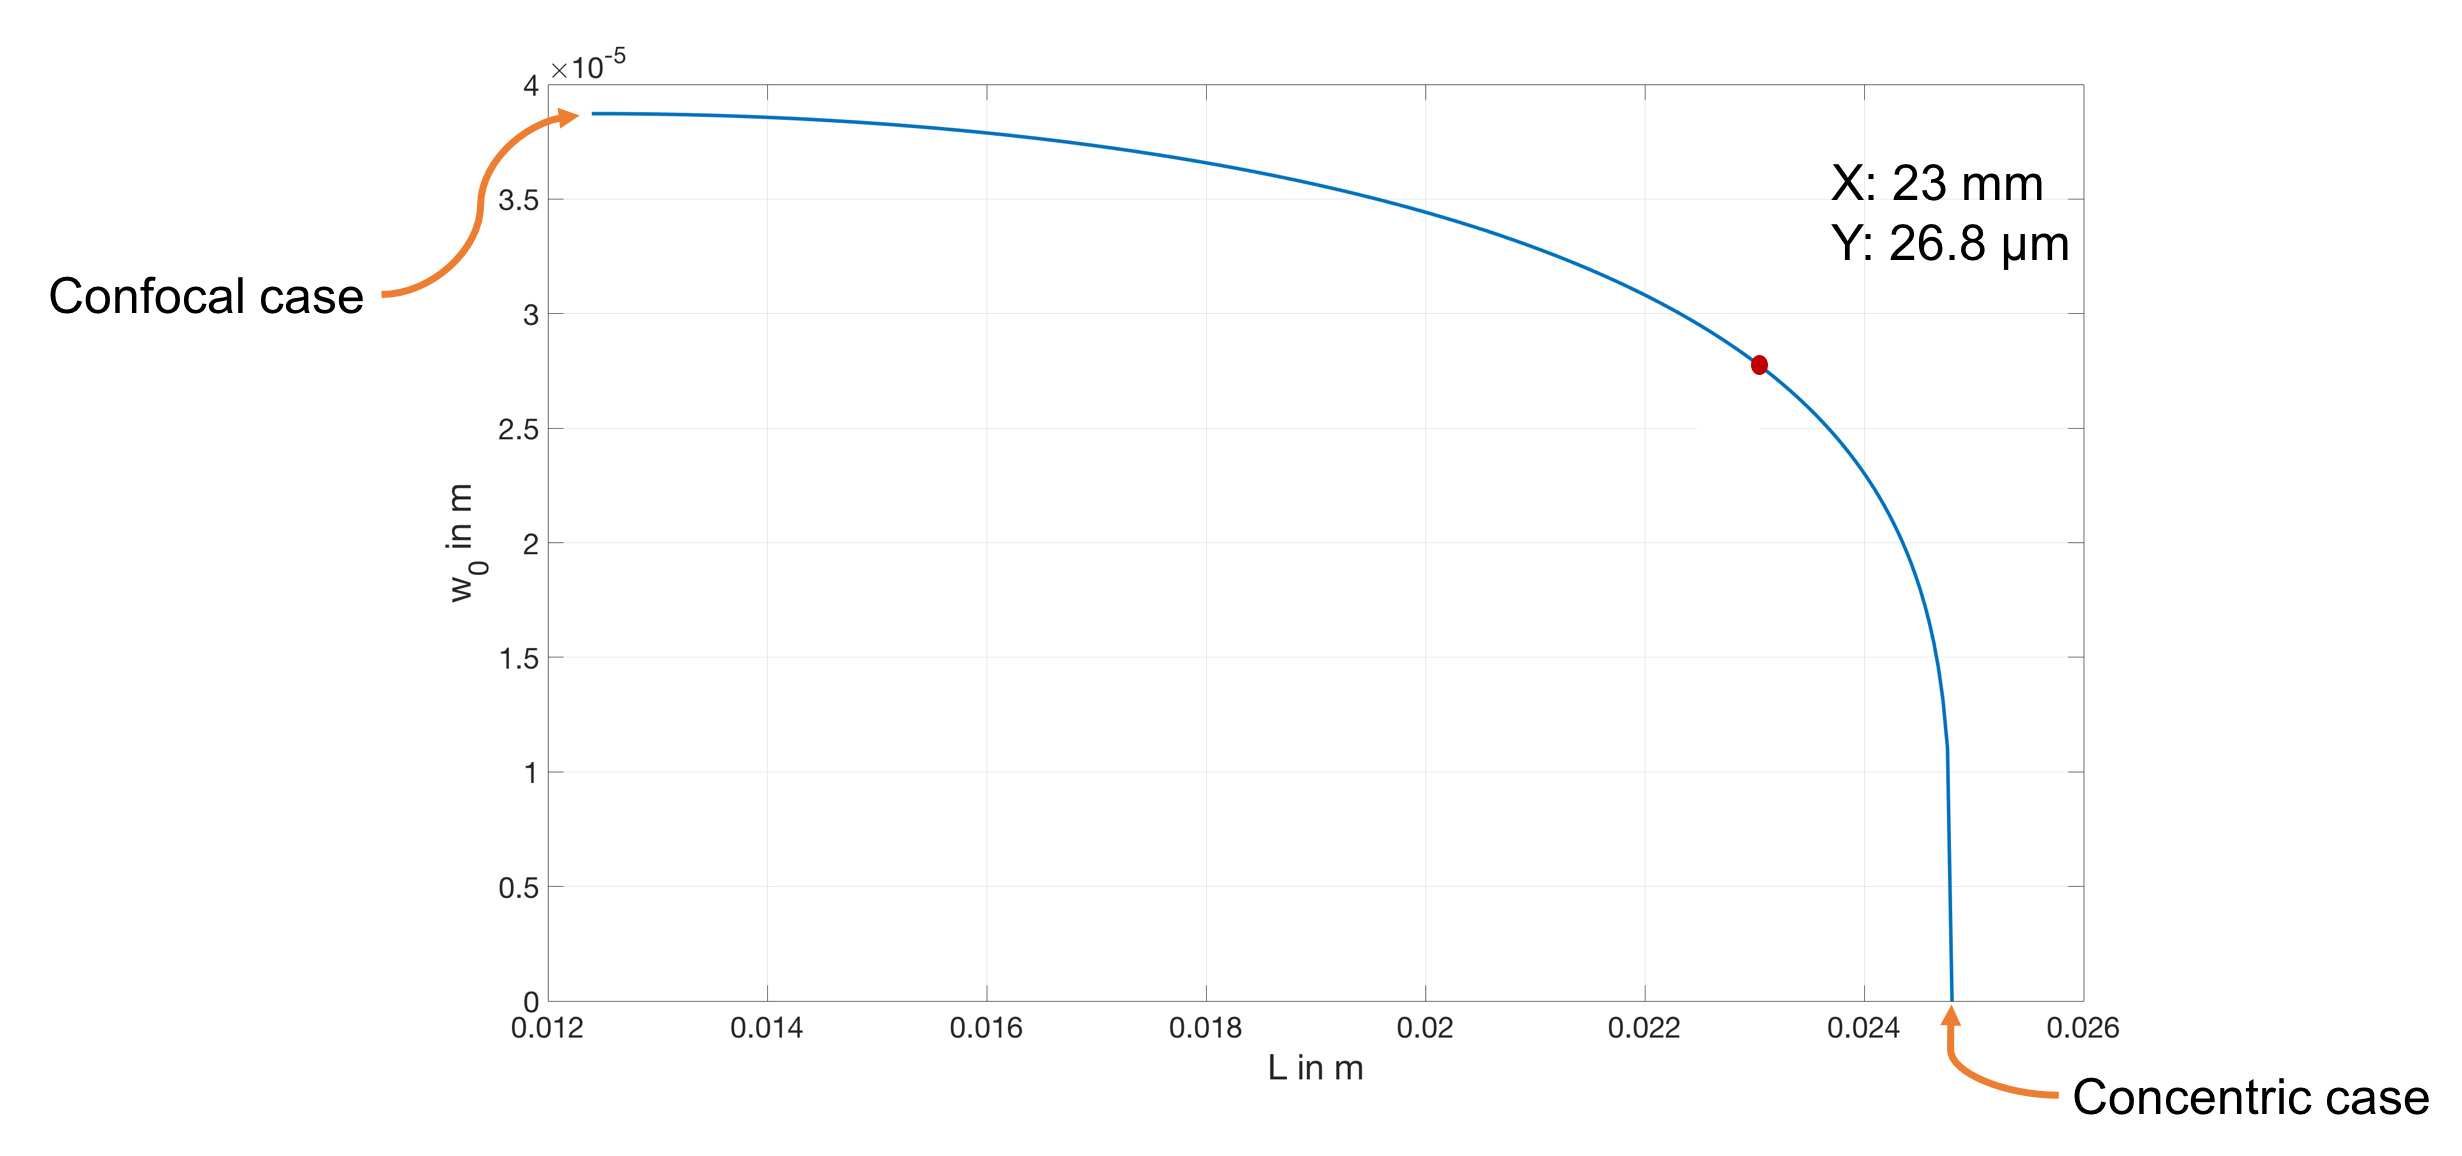
\includegraphics[ height=0.35\textheight]{05_OUSD/images/resLength.png}
	\caption{Waist radius in relation to the distance between the mirrors.}
	\label{fig:resLength}
\end{figure} 

The chosen distance between the mirrors were 23~$mm$. The red dot marks this point in Figure \ref{fig:resLength}. This value is as close to the confocal case as necessary, but distant enough to the concentric case to avoid instability, therefore the waistradius is 26.8~$\mu m$. 

\subsubsection{Mirror coating material considerations}

In order to find a suitable coating material and technique for the mirrors, some considerations have to be done. Primer terms are, that they can be coated at the institute and that the coating is durable against corrosion due to the alternating contact with water and air.\\
Therefore the physical vapor deposition (PVD) unit at the facility is chosen. In PVD a small cup, containing the selected metal, inside an evacuated chamber gets heated up to its evaporation temperature. The vaporized material spreads, due to its thermal energy, towards the target. The coating thickness is controlled by the exposure time of the target. Figure \ref{fig:CoatingMat} shows the spectral reflectivity, over a wavelength range from 200~$nm$ to 1200~$nm$, of materials that are eligible. 
 
\begin{figure}[H]
	\centering
	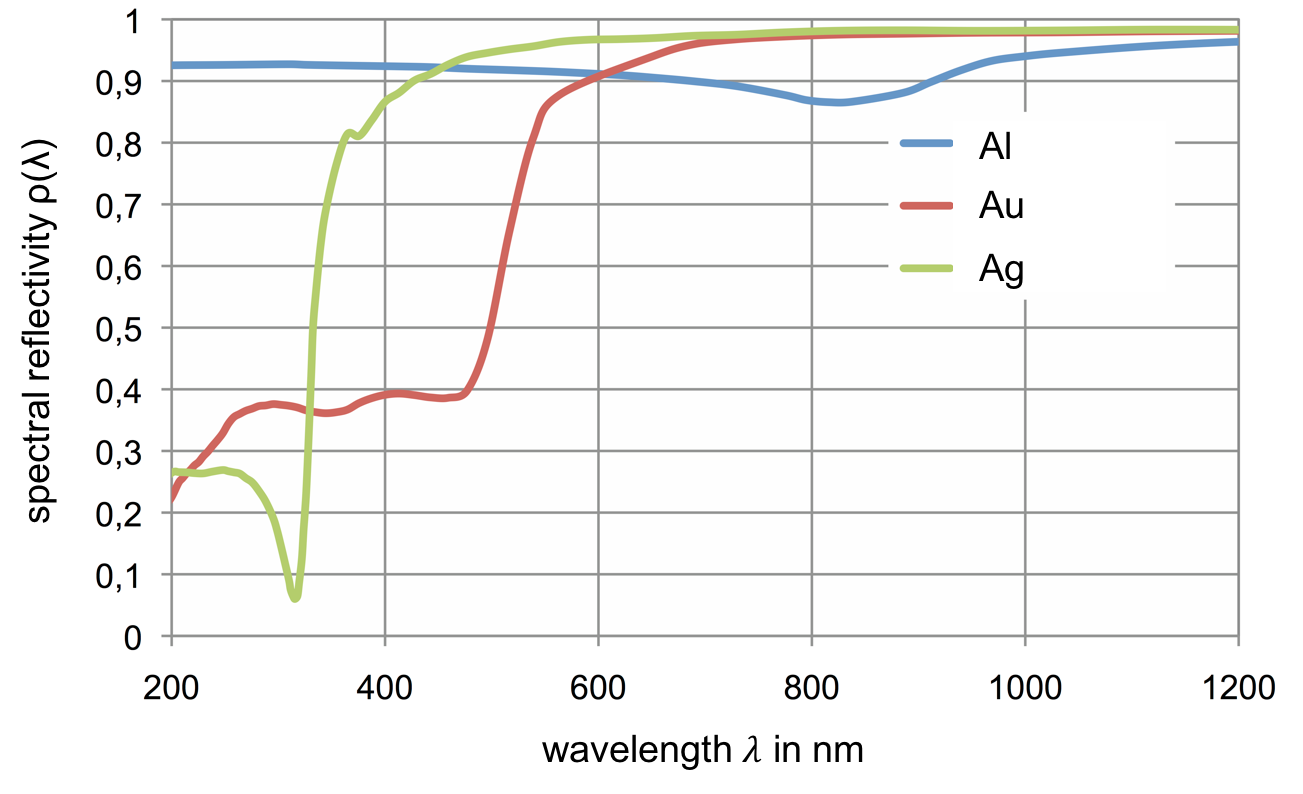
\includegraphics[width = 0.75\textwidth, height=0.3\textheight]{05_OUSD/images/coatingMat.png}
	\caption{Spectral reflectivity $\rho$ in dependence of the wavelength $\lambda$ for aluminum (Al), gold (Au) and silver (Ag).  \cite{bauelOptik}}
	\label{fig:CoatingMat}
\end{figure}

The chosen material should have a high reflectivity around 760~$nm$ and to be corrosion resistant. As gold has nearly the same reflectivity as silver at the desired wavelength, but a much higher durability, the chosen material for the mirror coating is gold. 

\subsubsection{Transfer matrix method (TMM)}

The calculation of an optical multilayer system can be done with the Transfer matrix Method. Especially the transmission and reflection of an optical multilayer system are of particular interest, to determine the the thickness of the gold layer. \\
Here the assumption is done that an incident beam is s-polarized and perpendicular to the plane. Besides that the layers are plain and expand infinite in z-direction. 
The Fresnel-coefficients are then given by

\begin{equation}
r_{ij} = \frac{n_i - n_j}{n_i + n_j};\; t_{ij} = \frac{2 \cdot n_i}{n_i + n_j}
\label{eq:r&t}
\end{equation}
\\
There $n$ is the complex refractive index $n = \tilde{n} + i \kappa$ that contains $\tilde{n}$, the refractive index and $\kappa$, the extinction coefficient. Furthermore, i is the current and j the following layer. 

\begin{figure}[ht]
	\centering
	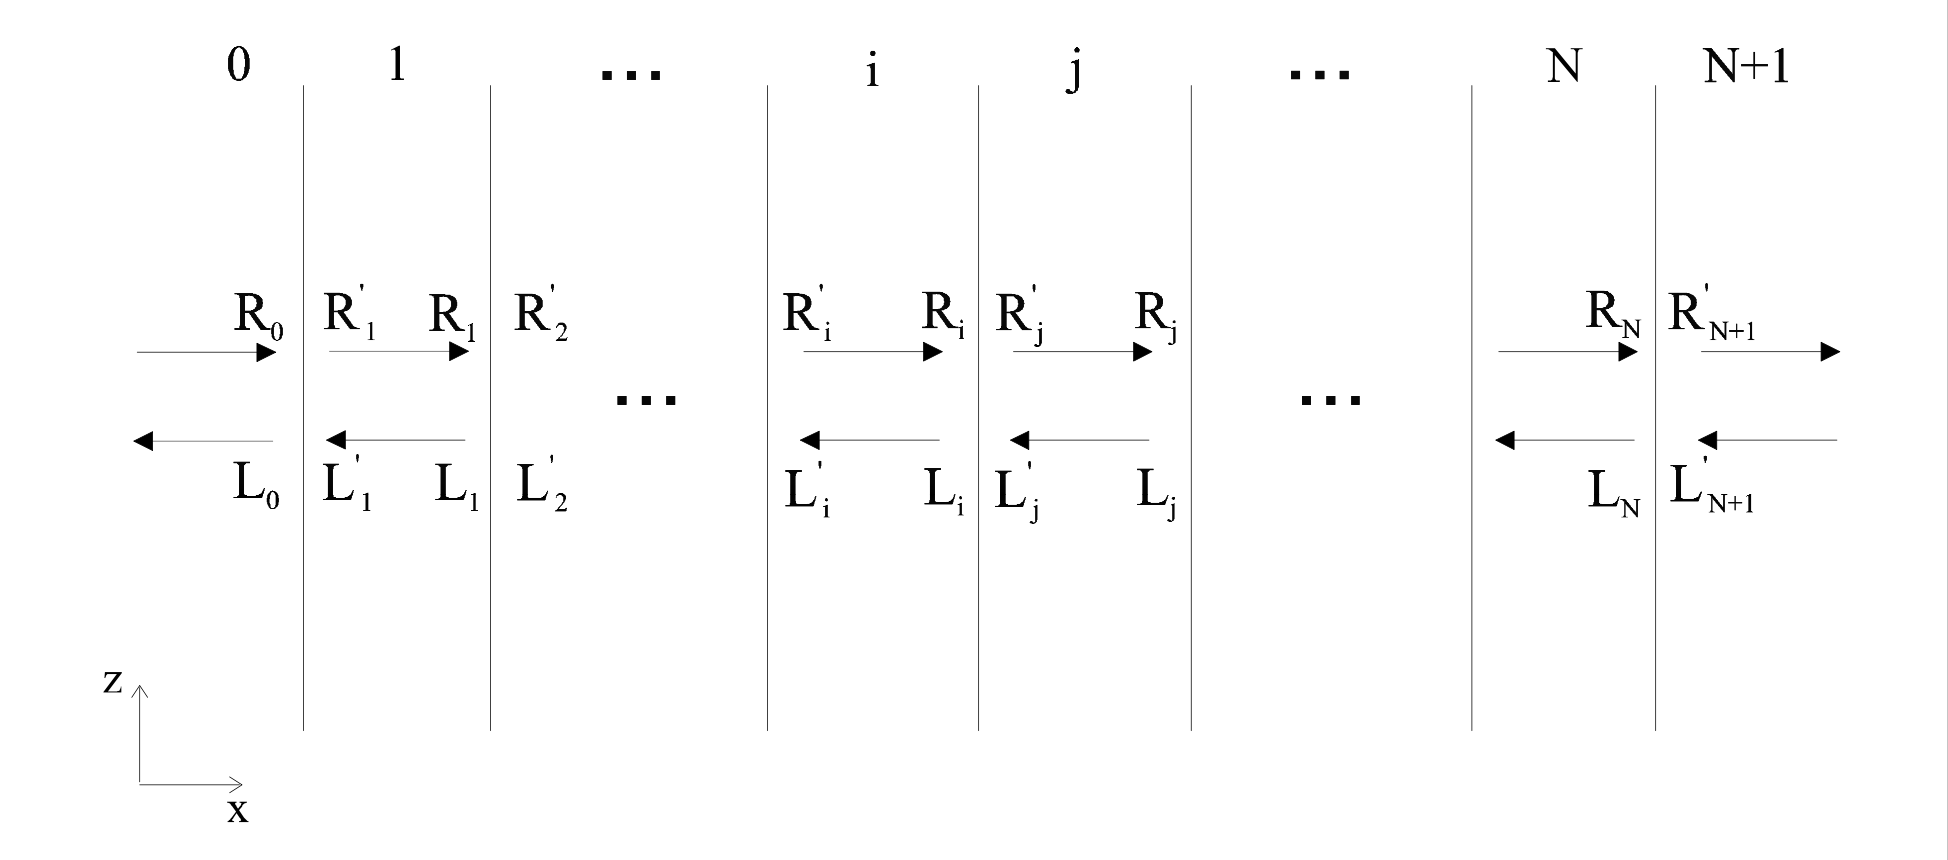
\includegraphics[width = 0.9\textwidth]{05_OUSD/images/SchemaSchichtsystem.png}
	\caption[Schematic of a layersystem]{Schematic view of a layer system \cite{Podgorsek:Vielfachschichten}}
	\label{fig:schemlayer}
\end{figure}

Figure \ref{fig:schemlayer} schematically shows the principle of a layer system. Every section contains a combination of left and right moving plane wave components. This sums up to a solution for the electrical field given by

\begin{equation}
E_i(x) = R_i\;exp(ik_{xi}x) + L_i\;exp(-ik_{xi}x) 
\label{eq:E_i}
\end{equation}
\\
where $ R_i $ is the ratio that goes in positive and $L_i$ in negative x-direction. \\
The left side of the boundary is defined by $ \begin{pmatrix}R_i \\ L_i\end{pmatrix} $  and $ \begin{pmatrix}R_j' \\ L_j'\end{pmatrix}  $ to the right. Based on the continuity condition, the amplitude vectors on both sides of the interface can be combined. 

\begin{equation}
\begin{pmatrix}R_i \\ L_i\end{pmatrix}  = \frac{1}{t_{ij}} \cdot 
\begin{bmatrix}
1 & r_{ij} \\ r_{ij} & 1
\end{bmatrix}  \begin{pmatrix}R_j' \\ L_j'\end{pmatrix}  = D_{ij} \begin{pmatrix}R_j' \\ L_j'\end{pmatrix} 
\label{eq:DMat}
\end{equation}
\\
$D_{ij}$ is the transfer matrix that describes the transition from layer $i$ to $j$. Inside a layer the vectors differ in a passing phase $\phi_i$.

\begin{equation}
\phi_i = k_0 \cdot n_i \cdot d_i
\label{eq:matKoeff}
\end{equation}
\\
Where $k_0$ is the incident wave vector, $n_i$ the complex refractive index of the current layer and $d_i$ the layer thickness. This phase is described by a phase matrix $P_i$

\begin{equation}
\begin{pmatrix}R_i' \\ L_i'\end{pmatrix}= 
\begin{bmatrix}
\exp(j \cdot \Phi_i) & 0 \\ 0 & \exp(-j \cdot \Phi_i)
\end{bmatrix}\begin{pmatrix}R_i \\ L_i\end{pmatrix}
= P_i \begin{pmatrix}R_i \\ L_i\end{pmatrix}
\label{eq:PMat}
\end{equation}
\\
This follows:
\begin{equation}
\begin{pmatrix}R_i' \\ L_i'\end{pmatrix}= 
P_i\;D_{ij} \begin{pmatrix}R_j' \\ L_j'\end{pmatrix}
\end{equation}
\\
Next a total transfer matrix $M$ is defined. It consists the product of all transfer($D$) and phase($P$) matrices to describe a layer system of $N$ layers

\begin{equation}
\begin{pmatrix}R_0 \\ L_0\end{pmatrix}
= M \;  \begin{pmatrix}R_{N+1}' \\ L_{N+1}' \end{pmatrix}
\label{eq:v0linkTovN+1}
\end{equation}

\begin{equation}
M = \begin{bmatrix}
M_{11} & M_{12} \\ M_{21} & M_{22}
\end{bmatrix} 
= D_{01} \cdot \prod \limits_{i=1}^{N} P_i \; D_{i, i + 1} 
\label{eq:matTMM}
\end{equation}
\\
By means of M, it is possible to calculate R and T. In order to do so, a wave hitting the layer system with amplitude $R_0$ and $L_{N+1}' = 0$, as shown in Figure \ref{fig:schemlayer}, can be supposed. Due to that, equation \eqref{eq:v0linkTovN+1} can be written as

\begin{equation}
R_0 = M_{11} \cdot R_{N+1}' \; ; \; L_0 = M_{21} \cdot R_{N+1}'
\end{equation}
\\
Therefore, the reflection and transmission coefficient are given by

\begin{equation}
r = \frac{L_0}{R_0} = \frac{M_{21}}{M_{11}} \; ; \;
t = \frac{R_{N+1}'}{R_0} = \frac{1}{M_{11}} 
\label{eq:rtCoef}
\end{equation}
\\
Finally R and T are determined:

\begin{equation}
R = \left\lvert \frac{M_{21}}{M_{11}}\right\rvert^2 \; ; \;
T = \left\lvert \frac{1}{M_{11}}\right\rvert^2
\label{eq:RT}
\end{equation}
\\
Therefore R and T depend on the wavelength, thickness of the layer and the complex reflection index that contains the extinction coefficient \cite{Podgorsek:Vielfachschichten}.

\subsubsection{Coating thickness determination with TMM}

In order to manufacture partially transmitting mirrors that fit into the system, a simulation were done with the help of the TMM. In figure \ref{fig:TMMsimLayersystem} the involved materials and their arrangement are shown . 

\begin{figure}[H]
	\centering
	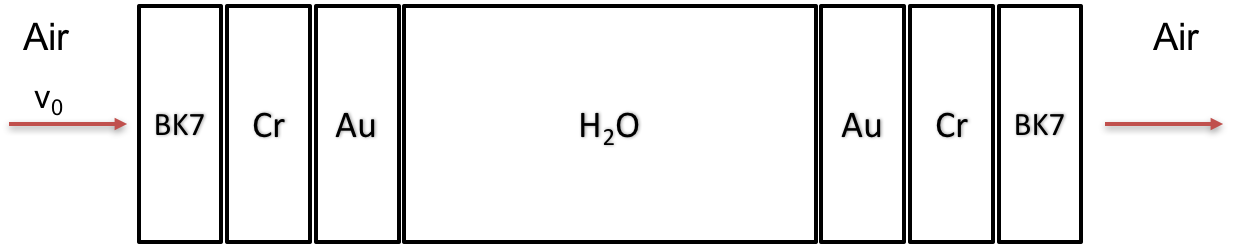
\includegraphics[height=0.15\textheight,width=\textwidth]{05_OUSD/images/TMM_schematisch.png}
	\caption{Schematic view of simulated layer system. The gold layer is variable, the others are fixed. For BK7 = 3.5~$mm$, Cr = 2~$nm$ and for H$_2$O = 23~$mm$.}
	\label{fig:TMMsimLayersystem}
\end{figure} 

The first layer is an air layer where the incident beam hits the system. Next one is the BK7 glass lens blank where the metals are coated onto. As those are concave, their waist thickness were taken. The chrome layer acts as an adherence layer for the following gold layer, but it barely affects the properties of the mirrors, due to the thickness of just a few atom layers. The H$_2$O layer has the thickness that was determined before in section \ref{sec:resLength}. At the end the vise versa configuration of the first mirror were established. The values for the complex refractive indexes are taken from the refractive index database \cite{rii}. The layer system from figure \ref{fig:TMMsimLayersystem}, were simulated in figure \ref{fig:transmission3D}, for a gold layer thickness range of 5~$nm$ to 70~$nm$.

\begin{figure}[H]
	\centering
	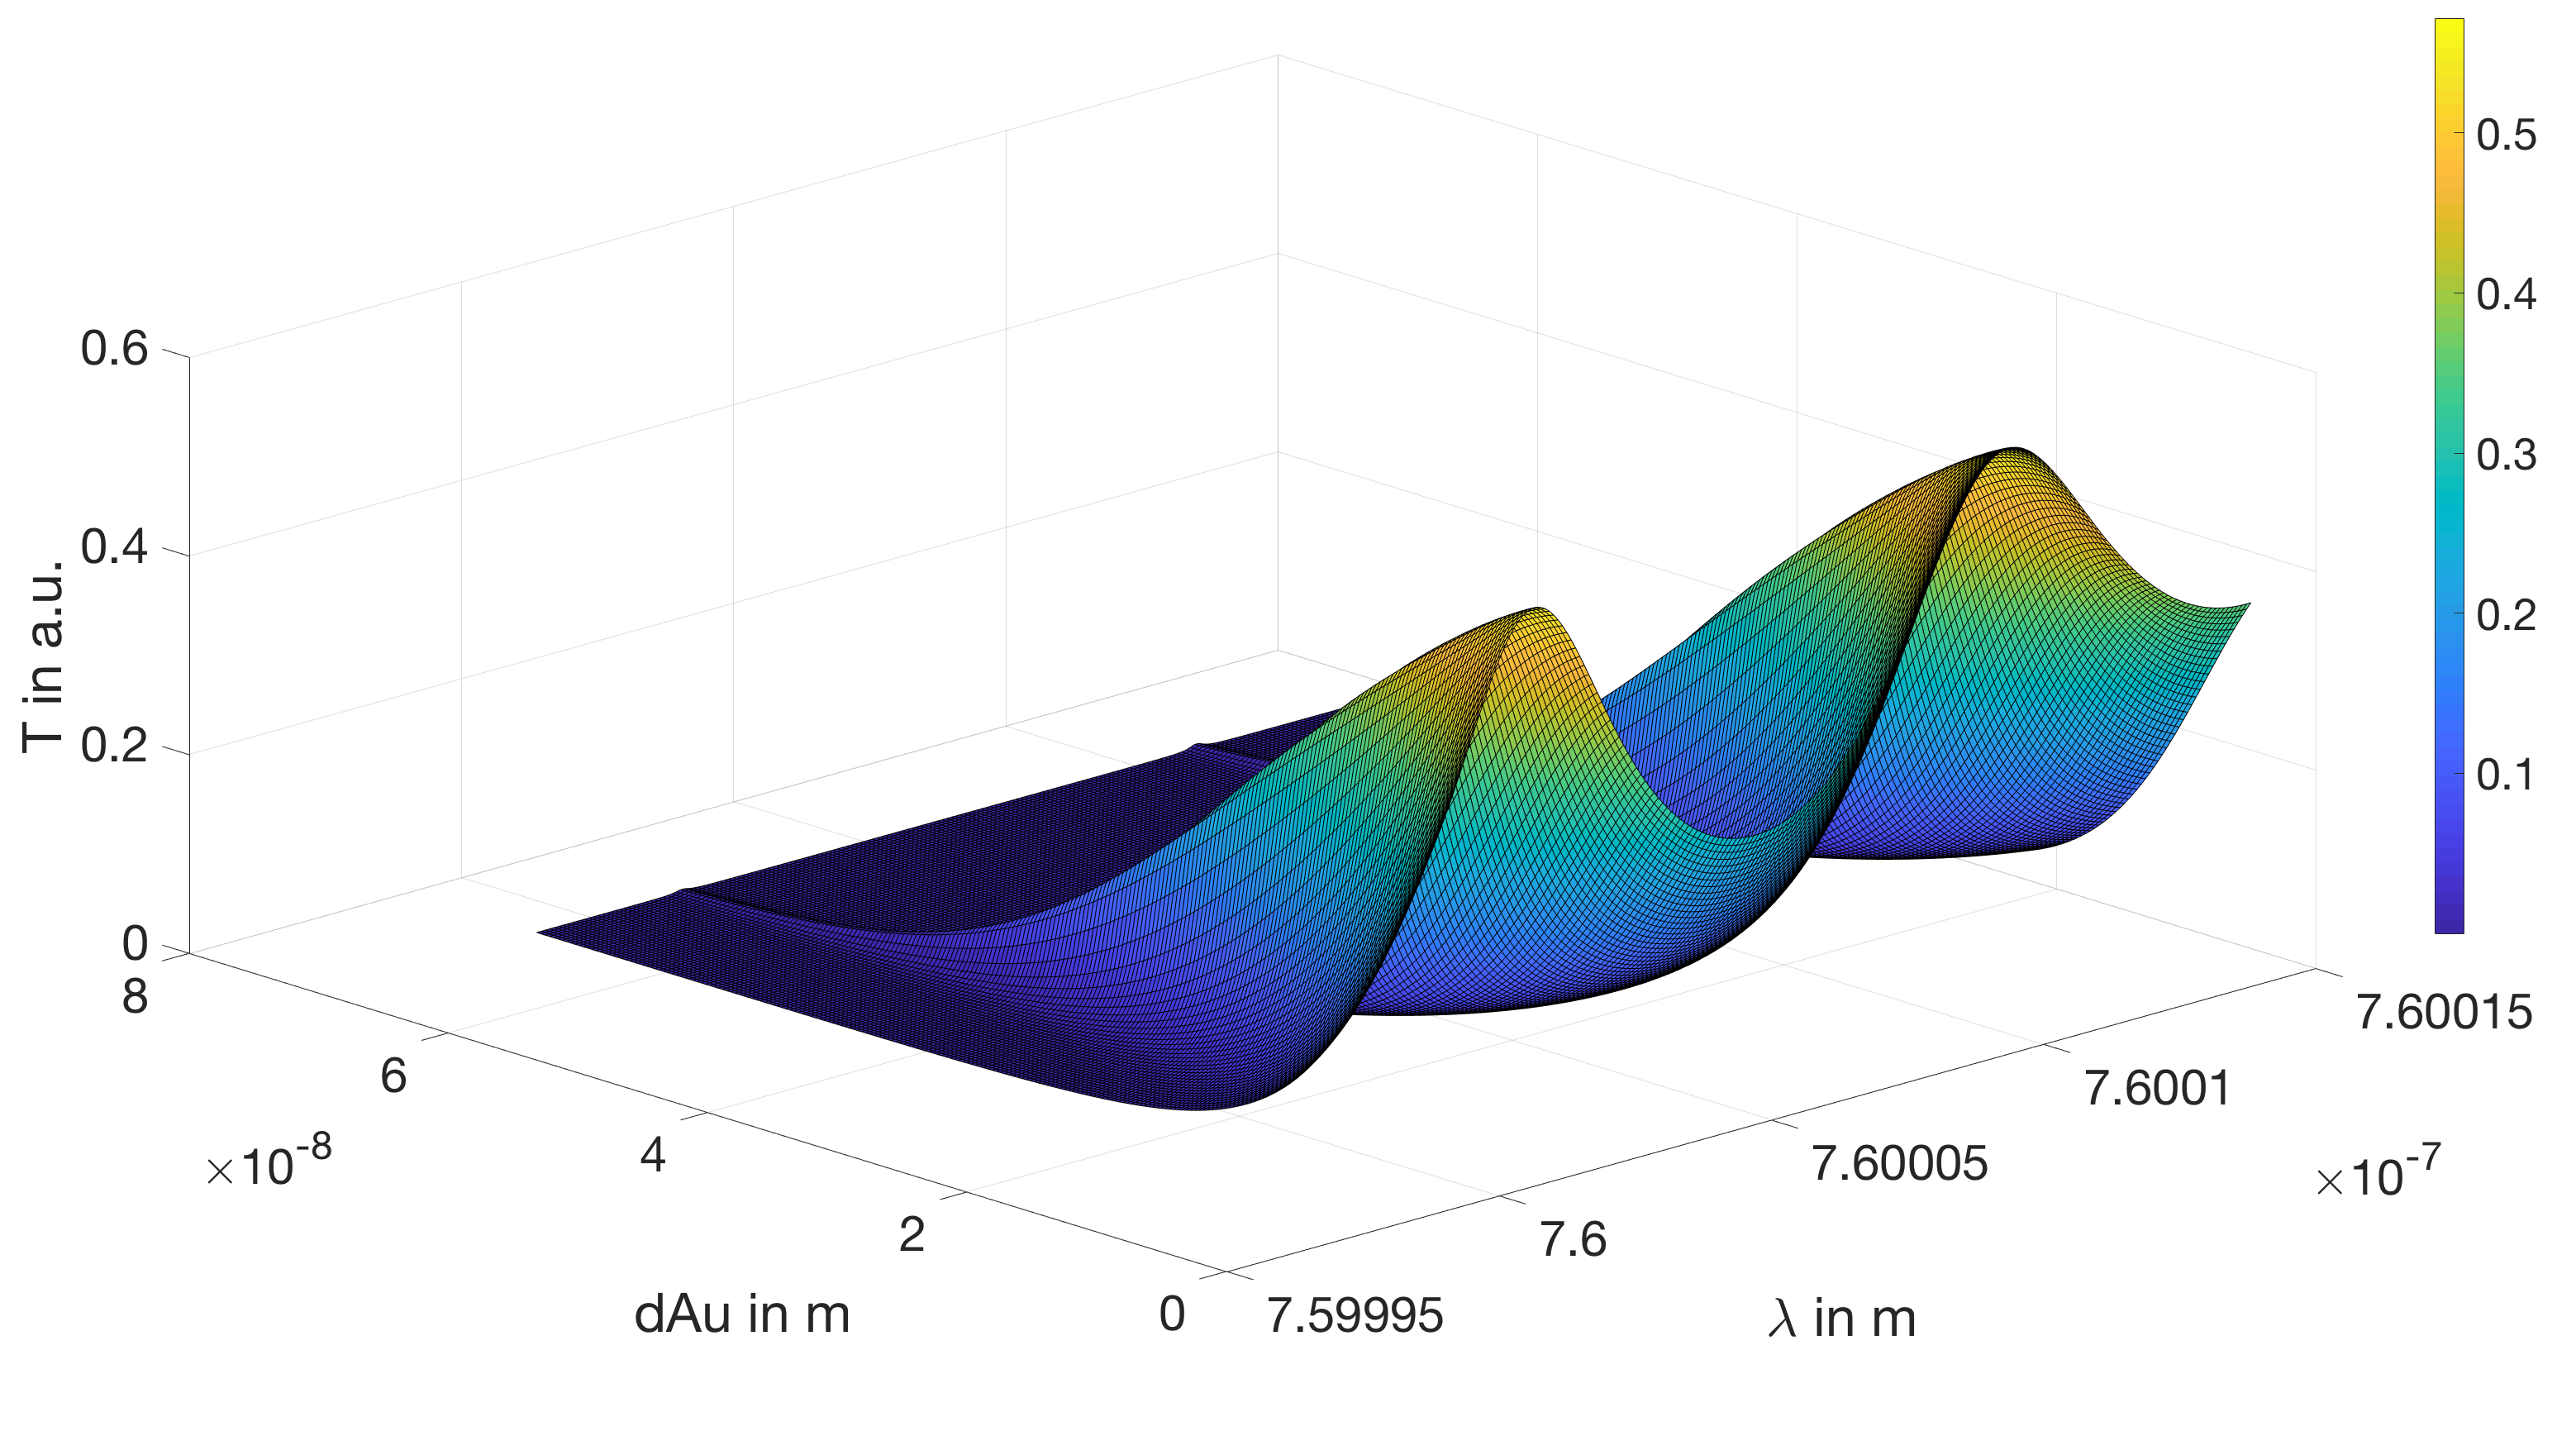
\includegraphics[height=0.47\textheight,width=\textwidth]{05_OUSD/images/transmission3D.png}
	\caption{Transmission pattern around the center frequency of the tunable laser in dependence of the gold layer thickness. The heatmap shows the transmission axis T in terms of color. The simulation were done with 200 points.}
	\label{fig:transmission3D}
\end{figure} 

As it can be seen, with increasing thickness of the gold layer, the transmission value decreases. For ultrasound detection the important value is the edge steepness of the transmission peaks. Figure \ref{fig:transDerivative} shows the maximum steepness values $\frac{\mathrm{d}T}{\mathrm{d}\lambda}$ dependent on the thickness of the gold layers.

\begin{figure}[H]
	\centering
	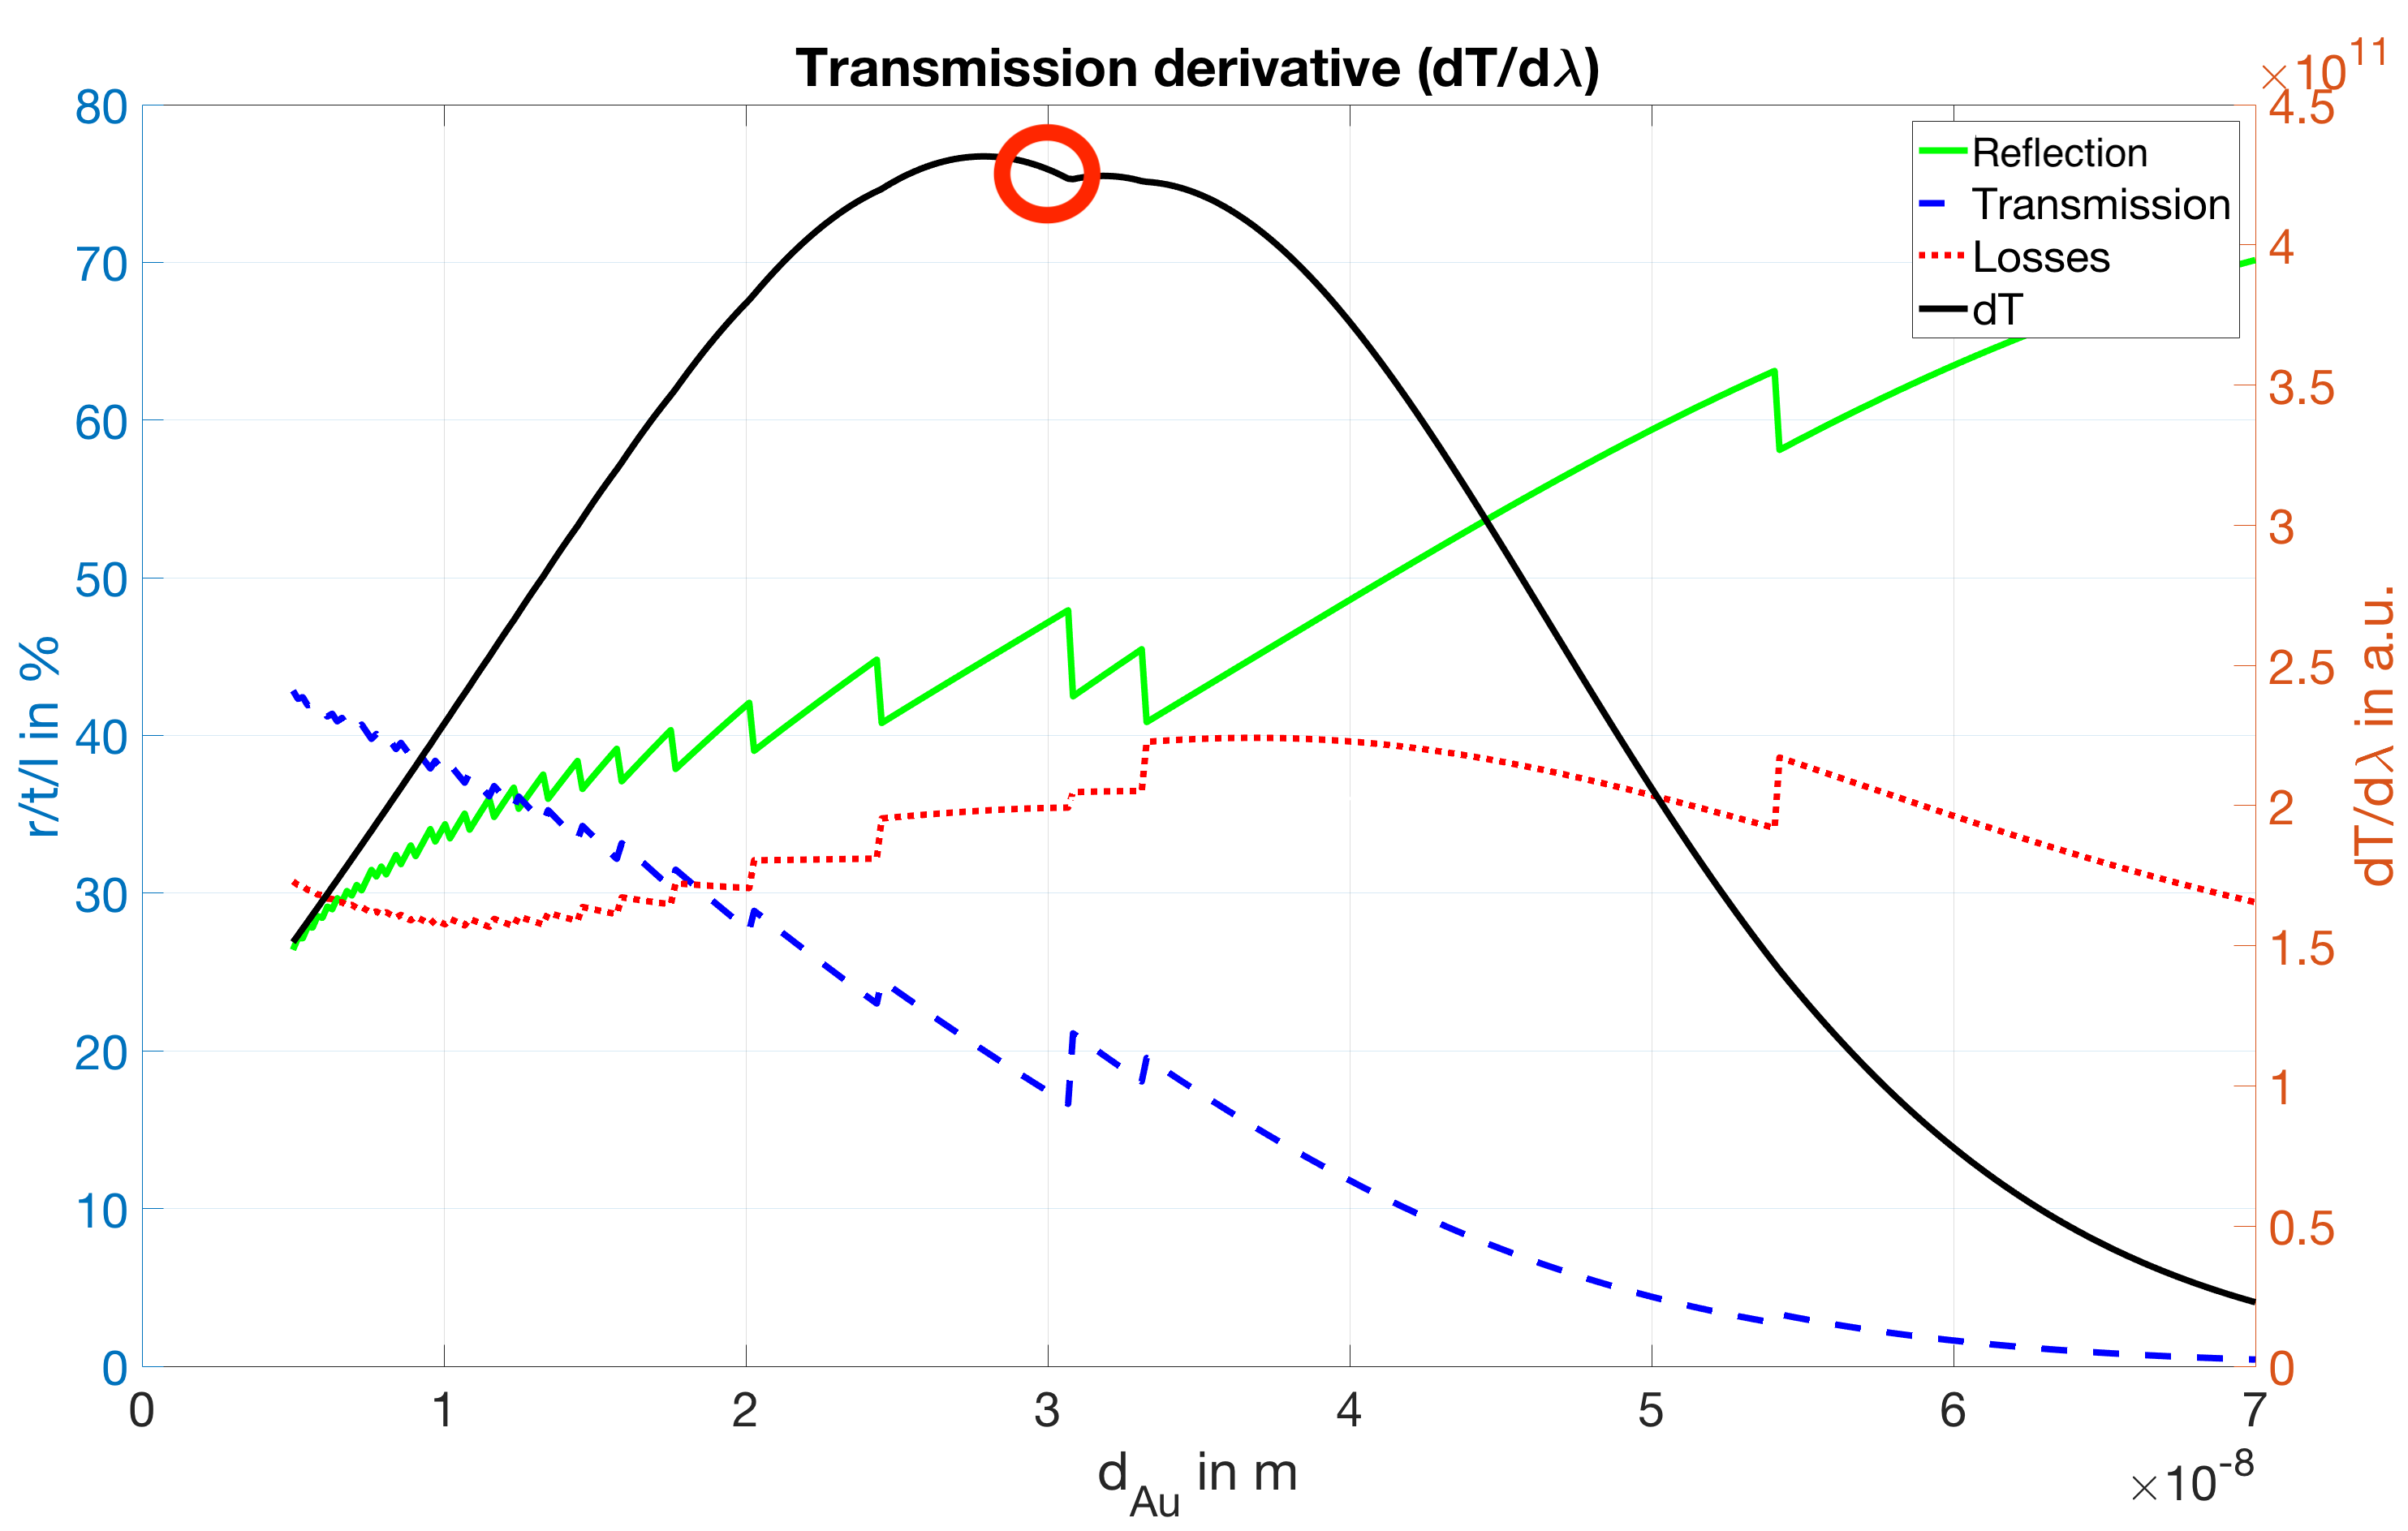
\includegraphics[height=0.56\textheight,width=1.1\textwidth]{05_OUSD/images/transDerivative.png}
	\caption{The black line shows the maximum values for the derivative of the transmission at a specific thickness of the gold layer and its corresponding axis is the right one. The values for transmission, reflection and losses are calculated based on this data. Besides the corresponding axis is the left one. The simulation were done with 200 points.}
	\label{fig:transDerivative}
\end{figure} 

The jumps in the lines for transmission, reflection and losses are a result of the varying points of maximum steepness. As there are two transmission peaks are considered in figure \ref{fig:transmission3D}, the maximum can either be at the first or second peak.\\
The maximum for $\frac{\mathrm{d}T}{\mathrm{d}\lambda}$, in figure \ref{fig:transDerivative}, is at about 30~$nm$ (red circle), therefore the mirrors were coated with this thickness value.  

\subsection{Cutoff frequency estimation}
\label{sec:cutOffFreq}

In order to estimate the cutoff frequency of the system, it can be assumed, that the light intensity in the middle of the resonator is rectangular distributed, as an approach to a Gaussian distribution, as illustrated in figure \ref{fig:lightDist} b). Therefore the width $d$ correspond to the FWHM of the cross section.  

\begin{figure}[H]
	\centering
	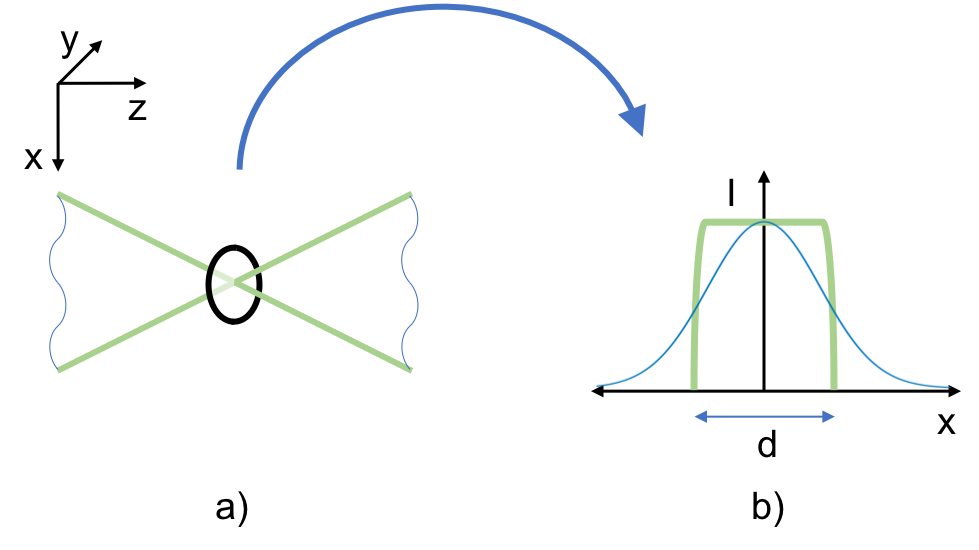
\includegraphics[height=0.4\textheight]{05_OUSD/images/lightDistribution.png}
	\caption{In a) the intersect of the mirror focuses is shown. The investigated cross section is marked. Furthermore, the origin lies in the center of the circle in a) and b) shows the supposed light distribution.}
	\label{fig:lightDist}
\end{figure} 

This allows us to simplify the calculation. The shortest incoming pressure wave has to have a wavelength of $\lambda/2$ because the change of the refractive index, whether the amplitude is positive or negative, is directed in one direction. For example, a full wavelength would cancel out the change of the refractive index because of the positive and negative amplitude. Therefore $\lambda$ has to be $\lambda_{cutoff} = 2 \cdot d$. This follows the equation

\begin{equation}
f_{cutoff} = \frac{c_{H_2O}}{\lambda_{cutoff}} =\frac{c_{H_2O}}{4 \cdot w_0}
\label{eq:fCutoff}
\end{equation}
\\
where $c_{H_2O}$ is the speed of sound in water at a given temperature and $w_0$ is the calculated waist radius. With the values for $c_{H_2O}$ = 1483.2~$m/s$ at 20~$^\circ C$ \cite{Haynes:physicalProperties} and as calculated in for in section \ref{sec:resLength}, $w_0$ = 26.8~$\mu m$, the cutoff frequency becomes $f_{cutoff}$ = 13.8~$MHz$. The actual value may be at a higher frequency due to the Gaussian beam profile. 

\subsection{Measuring-methods to determine the ultrasonic pressure}
\label{sec:pMeasureMeth}
In order to get an idea about the pressure amplitude range of the ultrasonic transducers that were used to determine the transfer function, two measurement setups were built. The first method were a needle hydrophone, there the ultrasonic field gets detected punctual and the second one is based on a Mach-Zehnder interferometer. Where the pressure amplitude is integrated over a line just like the OUSD system does. 
 
\subsubsection{Needle hydrophone}

A needle hydrophone is a PVDF foil which is glued on top of a metal tube. For this setup the Müller-Platte Nadelsonde from Dr. Müller Instruments were used, there the tip has a cross section of 1.2~$mm$. Figure \ref{fig:needleHydrophone} shows the measurement setup. 

\begin{figure}[H]
	\centering
	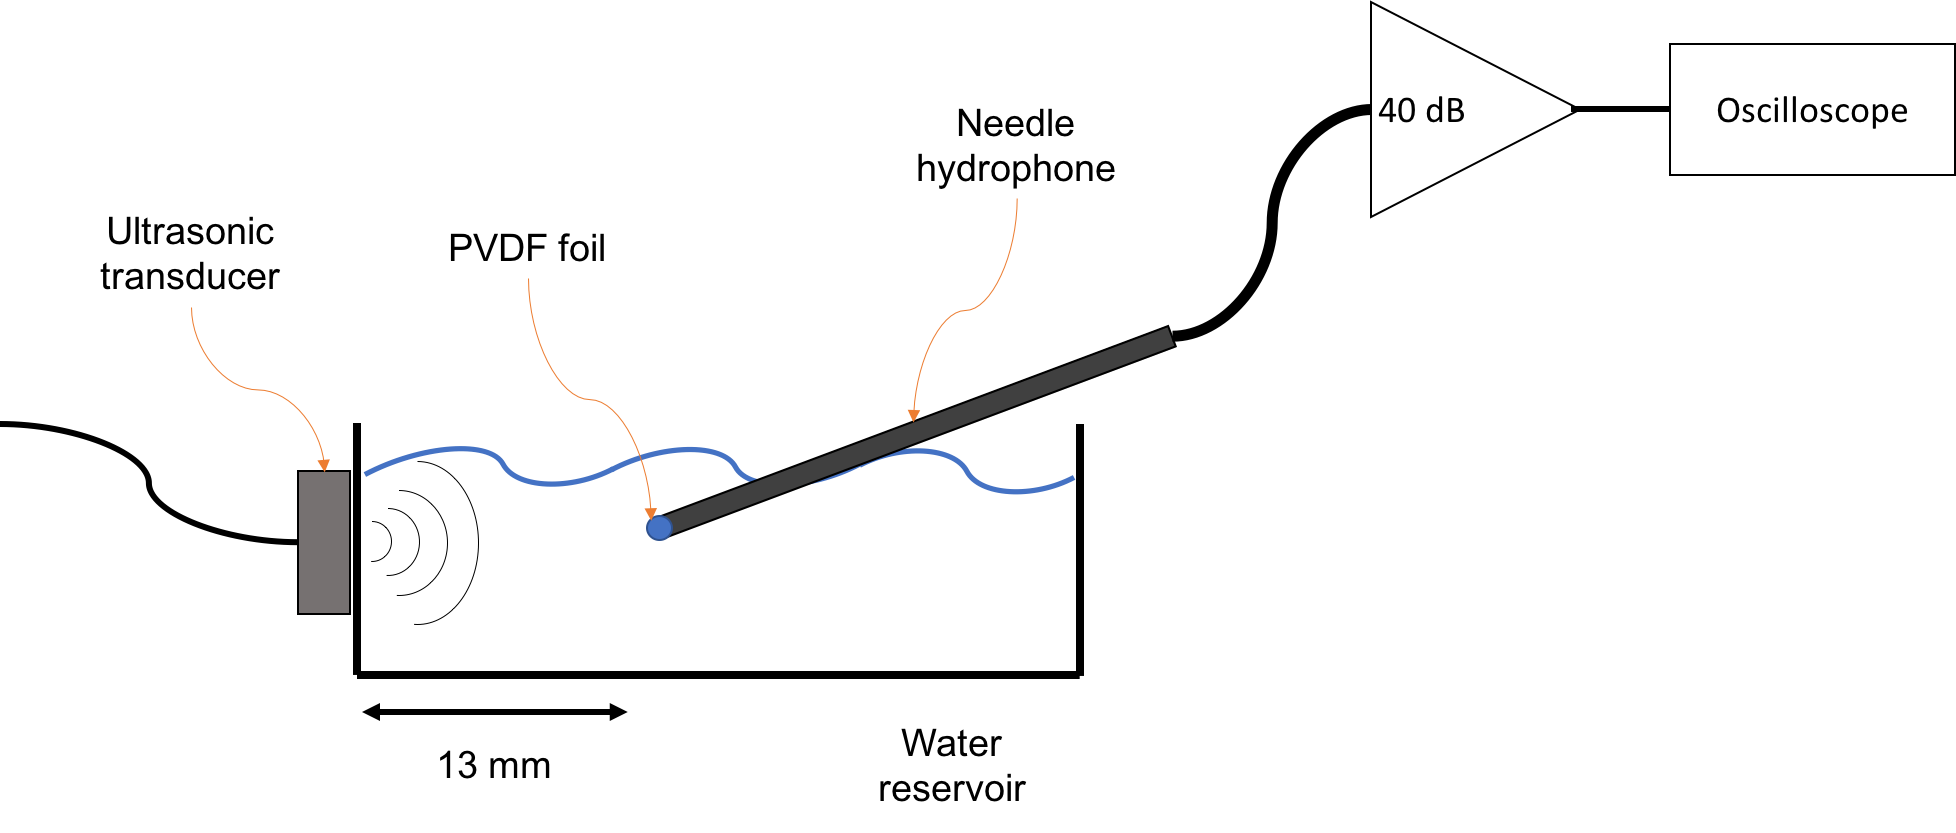
\includegraphics[width = \textwidth, height=0.3\textheight]{05_OUSD/images/NeedleHydro.png}
	\caption{Schematic of a needle hydrophone setup.}
	\label{fig:needleHydrophone}
\end{figure} 

The ultrasonic transducer were acoustically coupled onto the water reservoir, there the needle hydrophone were placed 13~$mm$ away from the transducer. This is about the working distance between the sample and the optical path of the detection laser in the OUSD system. \\
The ultrasonic wave that were detected gets amplified and displayed by an oscilloscope. With a conversion relation (here the sensitivity is 1.3~$\frac{mV}{bar}$) the voltage signal were translated into a pressure signal.  


\subsubsection{Mach-Zehnder interferometer}

In order to verify the results of the needle hydrophone a Mach-Zehnder interferometer were built. Figure \ref{fig:MZinterSchem} shows the schematic measurement setup.  

\begin{figure}[H]
	\centering
	\includegraphics[height=0.4\textheight]{05_OUSD/images/MZinterSchem.png}
	\caption{Schematic of a Mach-Zehnder interferometer.}
	\label{fig:MZinterSchem}
\end{figure} 

A cw-laser with 532~$nm$ wavelength were split into two optical paths. The first one directly hits a second beam splitter and acts as a reference signal. The second one gets deflected by a mirror and guided through a water reservoir. Here the laser beam can interact with the ultrasonic wave of an ultrasonic transducer, which were also placed inside the reservoir. The distance in between were also chosen to be 13~$mm$. \\
Afterwards the second beam also hits the lower beamsplitter shown in figure \ref{fig:MZinterSchem}. The two beams then are guided towards a balanced amplified photodetector, PDB120A from Thorlabs, with two separate optical inputs.\\
If the water reservoir would not exist the intensity at the photodetector inputs "Monitor -" and "Monitor +" would follow the proportionality

\begin{equation}
I_- \sim \cos^2\left(\frac{\Phi}{2}\right) \; ;\; I_+ \sim \sin^2\left(\frac{\Phi}{2}\right) 
\label{eq:I+I-}
\end{equation}
\\
therefore a $\Delta\Phi = 0$ follows a maximum intensity at Monitor - and a minimum at Monitor +. The dependence of the phase shift between the two inputs is illustrated in figure \ref{fig:MZoutput}. 

\begin{figure}[H]
	\centering
	\includegraphics[height=0.4\textheight]{05_OUSD/images/MZoutput.png}
	\caption{Mach-Zehnder interferometer output function dependent on phase shift.}
	\label{fig:MZoutput}
\end{figure} 

In order to get the detector output signal shown in figure \ref{fig:MZoutput}, with the water reservoir inserted, a control loop were applied to the system. The operation point has to be in the steepest part of the linear region, shown in figure \ref{fig:MZoutput}. Therefore a mirror were mounted on a piezo transducer (upper right mirror in figure \ref{fig:MZinterSchem}) and used as an optical phase shifter.\\
Due to the refractive index of water changes in dependency to pressure, the phase between the optical paths of the Mach-Zehnder interferometer changes, too. This is given by

\begin{equation}
\Delta\Phi = k \cdot \frac{\partial n}{\partial p} \cdot \int_{0}^{L}p(x)\mathrm{d}x
\label{eq:MZphaseP}
\end{equation}
\\

there $k = \frac{2\pi}{\lambda}$ is the wave vector and $L$ is the interaction length. With the assumption that the incident pressure wave is a plane wave, as shown in figure \ref{fig:pInteract}, the pressure distribution over the interaction length  $L$ becomes constant.

\begin{figure}[H]
	\centering
	\includegraphics[width = 0.4\textwidth, height=0.2\textheight]{05_OUSD/images/pInteract.png}
	\caption{Schematic of the interaction between an ultrasonic pressure wave and laser beam.}
	\label{fig:pInteract}
\end{figure} 

Therefore equation \ref{eq:MZphaseP} reduces to 

\begin{equation}
\Delta\Phi = \frac{2\pi}{\lambda} \cdot \frac{\partial n}{\partial p} \cdot p \cdot L
\label{eq:MZphasePred}
\end{equation}
\\

The signal sequence shown in figure \ref{fig:MZoutput} is the light intensity that reaches the two optical photodetector inputs, but the measured voltage $U_s$ is the difference between Monitor - and Monitor +. This leads to 

\begin{equation}
\Delta\Phi \sim \frac{U_s}{2\cdot U_{cf}} 
\label{eq:MZpropUs}
\end{equation}
\\

there $U_s$ is the measured signal voltage, $U_{cf}$ is the conversion factor from light intensity to a voltage signal and the factor $2$ follows from the two inputs. \\
The working area of the intensity profile, shown in figure \ref{fig:MZoutput}, is the linear region of the $\sin^2(x)$ function and its range is $\frac{\pi}{2}$. Adding a modulation voltage $U_{mod}$ scaling follows

\begin{equation}
\Delta\Phi = \frac{U_s \cdot \pi}{4 \cdot U_{cf} \cdot c \cdot U_{mod}} 
\label{eq:MZeqUs}
\end{equation}
\\

there $c = 0.70711$ is the result of $c = \sin^2(\frac{3}{4}\pi) - \sin^2(\frac{1}{4}\pi)$ and defines the valid region of $U_{mod}$. Furthermore, $U_{mod}$ is the maximum voltage range of the photodetector output. The result of formula \ref{eq:MZphasePred} with formula \ref{eq:MZeqUs} and solving for $p$ follows

\begin{equation}
p = \frac{\lambda \cdot U_s}{16 \cdot U_{cf} \cdot c \cdot U_{mod} \cdot L \cdot \frac{\partial n}{\partial p}} 
\label{eq:MZp}
\end{equation}
\\

This formula converts the measured voltage signal $[V]$ into a equivalent pressure signal $[Pa]$. 








\section{Experimental results of the optical ultrasonic detection system}
\label{sec:OUSDresults}
Based on the calculations and considerations a system for optical ultrasonic detection was built. In the following measurements the results, that characterize the detector, are represented.

\subsection{Finesse}

An important value for the characterization of a FPI is its finesse $\mathcal{F}$. That is defined by

\begin{equation}
\mathcal{F} = \frac{\Delta f}{\mathrm{d} f}
\label{eq:finesse}
\end{equation}
\\
there $\Delta f$ is the distance between two modes and $\mathrm{d} f$ FWHM \cite{eichler:laser}. A higher value here means that more beams inside the resonator sum up with each other, before the light leaves the system.\\
In figure \ref{fig:finesseSimMax} a simulation were done with the values determined above. Therefore the calculated finesse is 14.05. This is the maximum possible finesse achievable with the built system and for a distance of 23~$mm$ between the mirrors.  

\begin{figure}[H]			
	\includegraphics[width = \textwidth, height=0.35\textheight]{06_ex-results_of_OUSD/images/calcFinesse.png}
	\caption{Simulated Transmission pattern for a 30~$nm$ gold layer. The points taken for the measurement of the maximum possible resonator finesse are circled.}
	\label{fig:finesseSimMax}
\end{figure}

It became apparent that the chosen value of 23~$mm$ were too close to the concentric case and therefore to instable. Beside that it is difficult to match the focal points of the mirrors with the flanges screws at that value. In order to determine a more suitable distance a test setup were built.\\
Therefore, the mirrors were mounted onto cage-system bars to change the distance between them. In order to vary the resonance condition one mirror were attached to a piezo-element, that were connected to a waveform generator and the other one were fixed. It is important to note that a laser with 532~$nm$ were used. The reflectivity of the gold coated mirrors is significantly lower compared to 670~$nm$ (see figure \ref{fig:CoatingMat}). However, the influence at this wavelength, to the distance determination, is minimal but the actual finesse value for the OUSD system is higher. \\

\begin{figure}[H]
	a)
	\begin{minipage}{\textwidth}
		\begin{center}		
		\includegraphics[width = 0.85\textwidth, height=0.3\textheight]{06_ex-results_of_OUSD/images/finesse532.png}
		\end{center}
	\end{minipage}
	b)
	\begin{minipage}{\textwidth}
		\vspace*{0.5cm}
		\begin{center}		
		\includegraphics[width = 0.85\textwidth, height=0.3\textheight]{06_ex-results_of_OUSD/images/measFinesse.jpg}
	\end{center}
	\end{minipage}
\caption{In a) a calculated transmission pattern for a mirror distance of 15~$mm$ is displayed. The finesse value is 4.54. Furthermore, b) shows a measured transmission pattern, the finesse is about 4 to 5.}
\label{fig:finesse}
\end{figure}

In figure \ref{fig:finesse} a) a simulation and in b) a measurement of the transmission pattern is shown. The distance between the mirrors were 15~$mm$. Furthermore, the calculated finesse value of figure \ref{fig:finesse} a) agrees with the measured one.\\
As shown in b) a triangular function, for the function generator, were used for the measurements. Due to the shape of the applied voltage the mirror movement follows and the interference condition changes.\\
It turned out that 15~$mm$ also works well in the OUSD system. At that value, the estimated cutoff frequency decreases to about 10~$MHz$, but the positioning of the partially transmitting mirrors and support optics, were easier.\\

\begin{figure}[H]
	a)
	\begin{minipage}[c]{\textwidth}	
		\begin{center}	
		\includegraphics[width = 0.85\textwidth, height=0.3\textheight]{06_ex-results_of_OUSD/images/finesse760.png}
	\end{center}
	\end{minipage}
	b)
	\begin{minipage}[c]{\textwidth}	
		\vspace*{0.5cm}
		\begin{center}
		\includegraphics[width = 0.5\textwidth, height=0.25\textheight]{06_ex-results_of_OUSD/images/res_air_piezo@1V.png}
	\end{center}
	\end{minipage}
	\caption{In a) the theoretical possible finesse value for $\lambda$ = 760~$nm$, a mirror distance of 15~$mm$ and water as material between the mirrors. Furthermore, in b) a measured transmission pattern of the OUSD setup is shown. The piezo-element, that moves the grating of the wavelength turnable laser, is sensitive to edged signal sequences, a sinusoidal waveform were chosen.}
	\label{fig:finesseMeas}
\end{figure}

Figure \ref{fig:finesseMeas} b) shows a measured signal of the OUSD with a mirror distance of 15~$mm$ and water as medium between the mirrors. Moreover, the tunable laser system with 760~$nm$ wavelength were used. The finesse is about 6 to 7.\\
To sum up the finesse values, determined in figure \ref{fig:finesse}, for the calculated and measured finesse value agree. Therefore the system were adjusted close to the theoretical maximum finesse value. However, the calculated value of 15.85 in figure \ref{fig:finesseMeas} a), for the actual OUSD setup, were not reached by the measured value in figure \ref{fig:finesseMeas} b). This is referred to the imprecise mirror mounting system, that uses four M2 screws on each flange to fix and position the mirrors.  

\subsection{Transfer function}
\label{sec:OUSDtf}

The transfer function describes the reaction of the OUSD system to an pressure wave with a certain frequency bandwidth. In order to analyze the behavior, four ultrasonic transducers with a defined frequency of 1~$MHz$, 2~$MHz$, 4~$MHz$ and 25~$MHz$ are acoustically coupled onto the system and the response was recorded.\\
The recorded signals were normalized to the maximum pressure amplitudes estimated with the needle hydrophone and the Mach-Zehnder interferometer. Therefore, table \ref{tab:pressureVal} shows the measured data, determined with the methods introduced in chapter \ref{sec:pMeasureMeth}.

\begin{table}[H]
	\centering
	\caption{Measured maximum pressure amplitude for a 1~$MHz$, 2~$MHz$, 4~$MHz$ and 25~$MHz$ ultrasonic transducer. The 25~$MHz$ value for the needle hydrophone is not available, because the cutoff frequency of this device is 10~$MHz$.}
	\begin{tabular}{| m{3cm} | c | c | c | c |}
		\hline
		\centering &1~$MHz$&2~$MHz$&4~$MHz$&25~$MHz$ \\ \hline
		\centering Needle hydrophone&4.37~$kPa$&8.77~$kPa$&7.87~$kPa$&-\\ \hline
		\centering Mach-Zehnder \newline interferometer&4.23~$kPa$&5.79~$kPa$&8.56~$kPa$&8.91~$kPa$\\ \hline
	\end{tabular}

	\label{tab:pressureVal}
\end{table}
The system response to the ultrasonic transducers excitation is recorded and displayed in figure \ref{fig:transF}. The length between the mirrors is 15~$mm$.

\begin{figure}[H]			
	\includegraphics[width = \textwidth, height=0.4\textheight]{06_ex-results_of_OUSD/images/transF.png}
	\caption{Measured transfer function of the OUSD on a half logarithmic scale. The signal amplitudes are normalized to the needle hydrophone data (blue bars) and to the Mach-Zehnder-interferometer data (red bars). The yellow line marks a fit through the mean values and the -3~$dB$ value is marked by a red circle.}
	\label{fig:transF}
\end{figure}

The yellow line in figure \ref{fig:transF} is the fit function ($F_{fit}(f) = -9.2\cdot10^{-7}~\frac{1}{MHz} \cdot f + 2.8\cdot10^{-5}$) through the mean values. These are taken separately for each frequency, only the value for 25~$MHz$ is set to the value of the Mach-Zehnder interferometer. The 3~$dB$ cutoff frequency value is 15.04~$MHz$ which is higher than the estimated 10~$MHz$.\\
For a precise estimation of the cutoff frequency value more datapoints are necessary. But the estimated value lays in the area of the fitted data. 

\section{Conclusion}

This thesis investigates the Grueneisen effect, its application to photoacoustic microscopy and the comparison to optical resolution photoacoustic microscopy (OR-PAM). Furthermore, a setup to detect ultrasonic pressure waves by light is designed, built and characterized. \\
\\
Through a stepwise heating of OrangeG colored water and paprika powder colored rizinus oil, it is shown that the photoacoustic amplitude either rises (in case of water) or falls (in case of oil). This behavior is referred to the Grueneisen effect and is proven in figure \ref{fig:measuredGRproof}.\\
The dual pulse technique (section \ref{sec:dualPulseTechnique}) is introduced to make the Grueneiseneffect applicable to PAM. The images taken in section \ref{sec:ORGRcomp} show the additional possibilities of GR-PAM compared to OR-PAM, in particular the thermal contrast mechanism (figure \ref{fig:imgGRproof}) and the sectioning capabilities (figure \ref{fig:imgGRblackleaf}). Moreover, an improvement of 7~$\%$ in the lateral resolution, of GR-PAM in relation to OR-PAM, is determined. However, the theoretical improvement of $\sqrt{2}$ could not be reached.\\
Besides the travel time of the ultrasonic wave is used to gain structural information of different materials in OR-PAM (section \ref{sec:topoPAI}). Thereby the data of the black leaf sample is used to determine the sample tilt compared to the scan plane, shown in figure \ref{fig:sampletilt}.\\
In the second part a system, based on a Fabry–P\'{e}rot interferometer, is developed to detect ultrasonic pressure waves by light (section \ref{sec:OUSD}). The task was to built a compact and movable ultrasonic detector. This is realized by replacing the free jet implementation, of the excitation and detection laser supply, through optical fiber and reducing the size of the mirrors and housing (section \ref{sec:sysDev}). The functionality is tested and proved in section~\ref{sec:OUSDresults}. The built setup has a finesse of about 6 to 7 and a estimated cut off frequency of 15.04~$MHz$.
Additionally the maximum pressure amplitude of several ultrasonic piezo transducers is determined by a needle hydrophone and a Mach-Zehnder interferometer setup (table \ref{tab:pressureVal}). Overall, all requirements given for the work are met.\\ \\

In order to improve the scan speed of the OR-PAM setup, described in section \ref{sec:ORPAMsetup}, the positioning stages could be replaced by a scanning galvo mirror system. \\
During the operation of the OUSD the problem emerged that small air bubbles are accumulate at the center of the concave mirrors. This could be solved by a piezoelectric element in the $kHz$-range, which is coupled onto the system to degas the media between the mirrors. \\
A further improvement would be the use of dielectric-coated plano-concave mirrors for the Fabry–P\'{e}rot interferometer. This leads to an increased finesse and results in a higher sensitivity of the OUSD. \\
In order to work with mirror distances closer to the  concentric case (see figure \ref{fig:resStability} and \ref{fig:resLength}), a refine of the mirror mounting system would lead to a more preciser alignment.\\
This thesis shows a prove of concept for a compact OUSD system, though further characterization measurements towards the transfer function should be done to give a more precise value for the cutoff frequency.  \\ 
\\
 In summery, GR-PAM is an useful addition to common photoacoustical methods. It can provide additional information about a sample and increase the contrast, if substances with differing $G$ are included.\\
 Furthermore, the optical detection of ultrasonic pressure waves can contribute a good alternative to common piezoelectric transducers.

\pagebreak


\ifthenelse{\boolean{oddpage}}{}{\newpage	\thispagestyle{empty}	\section*{} \pagebreak}

\thispagestyle{empty}
\begin{minipage}[c][\textheight]	{\textwidth}
	\thispagestyle{empty}
	\begin{center}
	\addsec{\hfil Appendix }
	\end{center}
\end{minipage}

\pagebreak
\appendix
\renewcommand \thesubsection {\Roman{subsection}}



\renewcommand{\refname}{}
\subsection{Bibliography}

\refstepcounter{section} 
%\bibliographystyle{alphadin}
%\printbibheading
\printbibliography
%\bibliography{literature.bib}
\pagebreak

\renewcommand\listfigurename{}
\subsection{List of figures}
\listoffigures
\pagebreak

\renewcommand\listtablename{}
\subsection{List of tables}
\listoftables
\pagebreak

\subsection{List of Abbreviations}

\newcolumntype{P}[1]{>{\centering\arraybackslash}p{#1}}
\begin{center}
    \begin{tabular}{|  P{3cm} | p{10cm} | }
    \hline
    AC & Aluminum coating \\ \hline
    Ag  & Silver \\ \hline 
    Al & Aluminum \\ \hline
    Au & Gold \\ \hline
    AR-PAM & Acoustical resolution photoacoustic microscopy \\ \hline
    BK7 & Borosilicate glass \\ \hline
    BS & Beamsplitter \\ \hline
    $^\circ$C & Degree Celsius \\ \hline
    Cr & Chromium \\ \hline 
    cw & Continuous wave \\ \hline
    DAQ & Data acquisition \\ \hline
    dB & Decibel \\ \hline
    DG & Delay generator \\ \hline
    ESF & Edge spread function\\ \hline
    FPI & Fabry-P\'{e}rot-Interferometer \\ \hline
    FWHM & Full width half maximum \\ \hline
    GR-PAM & Grueneisen relaxation photoacoustic microscopy \\ \hline
    H$_2$O & Water \\ \hline  
    HT & Hilbert transformation\\ \hline
    MRT & Magnetic resonance tomography \\ \hline
    OR-PAM & Optical resolution photoacoustic microscopy \\ \hline
    OUSD & Optical ultrasonic detector \\ \hline
    Pa & Pascal \\ \hline
    PA & Photoacoustic amplitude \\ \hline
    PAM & Photoacoustic microscopy \\ \hline
    PAT & Photoacoustic tomography \\ \hline 
    PC & Personal computer \\ \hline  
    PVD & Physical vapor deposition \\ \hline
    PVDF & Polyvinylidenfluorid \\ \hline
    SNR & Signal to noise ratio\\ \hline
    SOL & Silicon oil for refractive index matching \\ \hline
    TMM & Transfer matrix method \\ \hline
    UT & Ultrasonic transducer \\ \hline
    2D & Two dimensional \\ \hline
    3D & Three dimensional \\ \hline  
    \end{tabular}
\end{center}
\pagebreak
\subsection{List of Symbols}

\newcolumntype{P}[1]{>{\centering\arraybackslash}p{#1}}
\begin{center}
	
    \begin{longtable}{|  P{3cm} | p{10cm} |  }
    \hline
    P$_{laser}$ & Laser power\\ \hline
    Q$_{laser}$& Laser pulse energy \\ \hline
    $\tau_{laser}$ & Pulse duration \\ \hline
    I$_{laser}$ & Irradiance \\ \hline
    A$_{laser}$ & Laser beam diameter \\ \hline
    $\exp(x)$ & Exponential function \\ \hline
    $\mu_a$ & Absorption coefficient \\ \hline
    $\tau_{th}$ & Thermal relaxation time \\ \hline
    $\lambda_t$ & Thermal diffusivity \\ \hline
    $\delta$ & Penetration depth \\ \hline
    $\delta'$ & Smallest illuminated dimension of a volume \\ \hline
    $c_s$ & Speed of sound \\ \hline
    T & Temperature \\ \hline
    p & Pressure \\ \hline
    B & Bulk modulus \\ \hline
    $\rho_0$ & Density \\ \hline
    $\beta$ & Volume expansion coefficient \\ \hline 
    $\Gamma$ & Grüneisen parameter \\ \hline
    F & Fluence \\ \hline
    C$_V$ & Heat capacity at constant volume \\ \hline
    C$_P$ & Heat capacity at constant pressure \\ \hline
    $\nabla$ & Nabla operator \\ \hline
    $\kappa$ & Isothermal compressibility \\ \hline    
    t & time \\ \hline
    $\delta(t)$ & Delta function \\ \hline
    $\theta(t)$ & Heaviside function \\ \hline
    R$_s$ & Radius of a spherical object \\ \hline
    f & Frequency \\ \hline
    d & Distance \\ \hline
    k & Wave vector \\ \hline
    V & Volume \\ \hline
    N & Number of datapoints \\ \hline
    $\mathcal{H}\{x(t)\}$ & Hilbert transformation of x(t) \\ \hline
    j &  Imaginary number \\ \hline 
    $Im\{x(t)\}$ & Imaginary part of x(t) \\ \hline
    $Re\{x(t)\}$ & Real part of x(t) \\ \hline
    cos(t) & Cosine function \\ \hline
    sin(t) & Sine function \\ \hline
    $\omega$ & Angular frequency \\ \hline
    $\eta_{th}$ & Heat conversion coefficient \\ \hline
    G & Grueneisenparameter change \\ \hline
    $k_{loss}$ & Conversion losses \\ \hline
    $w_0$ & Waist radius \\ \hline
    $z_R$ & Rayleigh length \\ \hline
    T (@ OUSD) & Transitivity \\ \hline
    R & Reflectivity \\ \hline
    $\lambda$ & Wavelength \\ \hline
    $\frac{\mathrm{d}n}{\mathrm{d}p}$ & Elasto-optical coupling factor \\ \hline
    L & Length \\ \hline
    n & refractive index \\ \hline
    $\Phi_i$ & Passing phase \\ \hline
    M & Matrix \\ \hline
    U & Voltage \\ \hline
    $\mathcal{F}$ & Finesse \\ \hline
    NA & Numerical aperture \\ \hline 
    \end{longtable}
\end{center}
\pagebreak
\subsection{Ultrasonic transducer datasheet}
\label{app:datasheetUST}

	\centering
	\includegraphics[ height=0.95\textheight, width=\textwidth]{08_appendix/files/datasheetUStransducer.pdf}


\subsection{Photoacoustic signal generation - simulation program}
\label{app:PAgen}
	\centering
\includegraphics[ page=1, height=0.95\textheight, width=\textwidth]{08_appendix/files/APPpulseSim.pdf}
\includegraphics[ page=2, height=0.95\textheight, width=\textwidth]{08_appendix/files/APPpulseSim.pdf}
\includegraphics[ page=3, height=0.95\textheight, width=\textwidth]{08_appendix/files/APPpulseSim.pdf}

\endgroup

\end{document}